\chapter{Heritability Estimation}
\label{heritabilityChapter}
% Need to stress that we are only calculating the narrow sense heritability
	\section{Introduction}
	The development of \gls{ldsc} \citep{Bulik-Sullivan2015} has allowed researchers to estimate the true contribution of common \glspl{SNP} to the variance in different diseases.	
	However, it is unclear how different sampling strategies (e.g. extreme phenotype selection) affects the performance of \gls{ldsc}.
	Additional simulations might therefore be required to investigate how different samplings affect the performance of \gls{ldsc}.
	
	The estimation of heritability on binary trait has always been complicated, as ascertainment bias correction is required when transforming the estimate on the binary scale to that on the liability scale.
	Nevertheless, the correction of ascertainment bias are nontrivial and can introduce bias to the estimates. 
	For example, \citet{Golan2014} observed that \gls{gcta} underestimates the heritability explained by common variants for case control studies.
	The magnitude of this bias is affected by a number of factors, including the population prevalence of the trait, the observed prevalence, the true underlying heritability and the number of genotyped \glspl{SNP} \citep{Golan2014}.
	As for case control samples, \citet{Bulik-Sullivan2015} only investigated the performance of \gls{ldsc} for traits with heritability of 0.8 and a population prevalence of either 0.1 or 0.01, more simulates are required in order to investigate whether if \gls{ldsc} suffers from the same bias as \gls{gcta}.
	
	Finally, as noted by \citet{Bulik-Sullivan2015}, when the number of causal variants is low, the standard error of the \gls{ldsc} estimate become very large, indicating that \gls{ldsc} is best suited to polygenic traits.
	This led to the need of developing an alternative algorithm that can be applied for various genetic architecture models.
	
	Herein, \gls{shrek}, an alternative algorithm to \gls{ldsc} for the estimation of \gls{SNP} heritability using \gls{GWAS} summary statistics was introduced.
	To examine the effect of different sampling strategies and genetic architectures on the performance of \gls{ldsc} and \gls{shrek}, extensive simulation were performed. 
	Moreover, to demonstrate that \gls{shrek} also works outside of simulated data, we also estimated the \gls{SNP} heritability of \glng{scz} and other psychiatric disorders using \gls{shrek}.
	
	The work in this chapter were done in collaboration with my colleagues who have kindly provided their support and knowledges to make this piece of work possible.
	Dr Johnny Kwan, Dr Miaxin Li and Professor Sham have helped to lay the foundation of this study. 
	Dr Timothy Mak has derived the mathematical proof for our heritability estimation method. 
	Miss Yiming Li, Dr Johnny Kwan, Dr Miaxin Li, Dr Desmond Campbell, Dr Timothy Mak and Professor Sham have helped with the derivation of the standard error of the heritability estimation. 
	Dr Henry Leung has provided critical suggestions on the implementation of the algorithm.
	
	\section{Methodology}			
		\subsection{Heritability Estimation}
			Given that the heritability ($h^2$) is defined as the proportion of total variance of the phenotype ($\boldsymbol{y}$) in a population explained by the variation of genetic factors ($\boldsymbol{x}$):
			$$
				h^2 = \frac{\mathrm{Var}(\boldsymbol{y})}{\mathrm{Var}(\boldsymbol{x})}
			$$
			
			In a typical \gls{GWAS}, regression is performed to test for an association between each \gls{SNP} and the phenotype of interest:
			\begin{equation}
				\boldsymbol{y}=\boldsymbol{\beta x}+\boldsymbol{\epsilon}
				\label{eq:standardRegress}
			\end{equation}
			where $\boldsymbol{y}$ and $\boldsymbol{x}$ are both standardized.
			$\boldsymbol{\epsilon}$ is defined as the error term, accounting for the non-genetic elements contributing to the phenotype (e.g. environment factors).
			By assuming $\beta \boldsymbol{x}$ to be independent of $\boldsymbol{\epsilon}$, one can transform \cref{eq:standardRegress} into:
			\begin{align}
				\mathrm{Var}(\boldsymbol{y}) = \mathrm{Var}(\beta \boldsymbol{x})+ \mathrm{Var}(\epsilon) \nonumber\\
				\mathrm{Var}(\boldsymbol{y}) = \beta^2\mathrm{Var}(\boldsymbol{x}) \nonumber\\
				\beta^2= \frac{\mathrm{Var}(\boldsymbol{y})}{\mathrm{Var}(\boldsymbol{x})}
				\label{eq:betaHeri}
			\end{align}
			As a result, $\beta^2$ represents the portion of phenotype variance explained by the variance of genotype.
					
			A challenge arises when calculating the heritability from \gls{GWAS} which only the summary statistic or p-value are available.
			When the genotype data is not accessible, estimation of $\mathrm{Var}(\boldsymbol{x})$ becomes infeasible, thus \cref{eq:betaHeri} cannot be used. 
			
			In order to estimate the \gls{SNP} heritability using \gls{GWAS} summary statistics, the estimation of the relative effect size of each individual \glspl{SNP} is necessary. 
			It was observed that when $\boldsymbol{x}$ and $\boldsymbol{y}$ are standardized, $\beta^2$ equals to the coefficient of determination ($r^2$). 
			Thus, based on properties of the Pearson product-moment correlation coefficient:
			\begin{equation}
				r = \frac{t}{\sqrt{n-2+t^2}}
				\label{eq:pearsonProduct}
			\end{equation}
			where $t$ follows the student-t distribution under the null and $n$ is the number of samples.
			The $r^2$ can then be obtained by taking the square of \cref{eq:pearsonProduct}
			\begin{equation}
				r^2 = \frac{t^2}{n-2+t^2}
				\label{eq:oriRSquared}
			\end{equation}
			Although $t^2$ follows the F-distribution under the null, it will converge into $\chi^2$ distribution when $n$ is large.
			
			Furthermore, when the effect size is small and $n$ is large, $n\times r^2$ becomes approximately $\chi^2$ distributed with mean $\sim 1$. 
			We can then approximate \cref{eq:oriRSquared} as
			\begin{equation}
				r^2= \frac{\chi^2}{n}
				\label{eq:approxChi}
			\end{equation}
			and define the \emph{observed} effect size of each \gls{SNP} to be
			\begin{equation}
			f=\frac{\chi^2-1}{n}
			\label{eq:observedEffect}
			\end{equation}
			
			However, when there are \gls{LD} between \glspl{SNP}, the situation will become more complicated as the observed effect of each \gls{SNP} is influenced by the neighboring \glspl{SNP} in \gls{LD} with it:
			\begin{equation}
			f_{observed} = f_{true}+f_{LD}
			\label{eq:conceptF}
			\end{equation}
			
			To account for the \gls{LD} structure, we first assume our phenotype $\boldsymbol{y}$ and genotype $\boldsymbol{x}=(x_1,x_2,\dots,x_m)^t$ are standardized such that
			\begin{align*}
				\boldsymbol{y}\sim f(0,1) \\
				\boldsymbol{x}\sim f(0,\boldsymbol{R})
			\end{align*}
			Where $f(m, \boldsymbol{V})$ denotes a general distribution with mean $m$ and variance $\boldsymbol{V}$ with $\boldsymbol{R}$ being the \gls{LD} matrix.
			
			We can then express \cref{eq:standardRegress} in matrix form:
			\begin{align}
				\boldsymbol{y}=\boldsymbol{\beta}^t\boldsymbol{x}+\epsilon
				\label{eq:matrixRegress}
			\end{align}
			Since the phenotype is standardized with variance of 1, the \gls{SNP} heritability can then be expressed as
			\begin{align}
				Heritability& = \frac{\mathrm{Var}(\boldsymbol{\beta}^t\boldsymbol{x})}{\mathrm{Var}(\boldsymbol{y})} \nonumber\\
				&=\mathrm{Var}(\boldsymbol{\beta}^t\boldsymbol{x})
			\end{align}
			If we then assume that $\boldsymbol{\beta} = (\beta_1, \beta_2,\dots,\beta_m)^t$ follows the distribution:
			\begin{align*}
				\boldsymbol{\beta}&\sim f(0,\boldmath{H})\\
				\boldsymbol{H}&=diag(\boldsymbol{h})\\
				\boldsymbol{h}&=(h_1^2,h_2^2,\dots,h_m^2)^t
			\end{align*}
			where $\boldsymbol{H}$ is the variance of the ``true'' effect. 
			Heritability can then be expressed as %The later part was gone because that will contains E(\beta) which = 0
			\begin{align}
			\mathrm{Var}(\boldsymbol{\beta}^t\boldsymbol{x}) &= \mathrm{E}_x\mathrm{Var}_{\beta|x}(\boldsymbol{\beta}^t\boldsymbol{x})+\mathrm{Var}_x\mathrm{E}_{(\beta|x)}(\boldsymbol{\beta}^t\boldsymbol{x}) \nonumber\\
			&=\mathrm{E}_x(\boldsymbol{x}^t\boldsymbol{\beta\beta}^t\boldsymbol{x}) \nonumber\\ 
			&= \mathrm{E}_x(\boldsymbol{x}^t\boldsymbol{Hx}) \nonumber\\
			&=\mathrm{Tr}(\mathrm{Var}(\boldsymbol{x}\boldsymbol{H})) \nonumber\\
			&=\sum_ih_i^2
			\label{eq:proveHerit}
			\end{align}
			
			Now if we consider the covariance between \gls{SNP}$_i$ ($\boldsymbol{x_i}$) and $\boldsymbol{y}$, we have
			\begin{align}
			 \mathrm{Cov}(\boldsymbol{x}_i,\boldsymbol{y}) &= \mathrm{Cov}(\boldsymbol{x}_i,\boldsymbol{\beta}^t\boldsymbol{x}+\epsilon) \nonumber\\
			 &=\mathrm{Cov}(\boldsymbol{x}_i,\boldsymbol{\beta}^t\boldsymbol{x}) \nonumber\\
			 &=\sum_j{\mathrm{Cov}(\boldsymbol{x}_i,\boldsymbol{x}_j)\boldsymbol{\beta}_j} \nonumber\\
			 &=\sum_j{\boldsymbol{R}_i\boldsymbol{\beta}_j}
			 \label{eq:covPhenoTrue}
			\end{align}
			
			As both $\boldsymbol{x}$ and $\boldsymbol{y}$ are standardized, the covariance equals to the correlation and we can define the correlation between \gls{SNP}$_i$ and $Y$ as
			\begin{equation}
				\rho_i = \sum_j{R_{ij}\boldsymbol{\beta}_j}
				\label{eq:corPhenoTrue}
			\end{equation}
			In reality, the \emph{observed} correlation is usually errors-prone. 
			Therefore we define the \emph{observed} correlation between \gls{SNP}$_i$ and the phenotype to be:
			\begin{equation}
			\hat{\rho_i} = \rho_i+\frac{\epsilon_i}{\sqrt{n}}
			\label{eq:obsPheno}
			\end{equation}
			for some error $\epsilon_i$. 
			The distribution of the correlation coefficient about the true correlation $\rho$ is approximately
			$$
				\hat{\rho_i}\sim f(\rho_i, \frac{(1-\rho^2)^2}{n})
			$$
			By making the assumption that $\rho_i$ is close to 0 for all $i$, we have 
			\begin{align*}
				\mathrm{E}(\epsilon_i|\rho_i)&\sim 0\\
				\mathrm{Var}(\epsilon_i|\rho_i)&\sim 1
			\end{align*}
			We then define our $z$-statistic and $\chi^2$-statistic as
			\begin{align*}
				z_i &= \hat{\rho_i}\sqrt{n} \\
				\chi^2_i &= z_i^2\\
				&=\hat{\rho_i}^2n
			\end{align*}
			From \cref{eq:obsPheno} and \cref{eq:corPhenoTrue}, $\chi^2$ can then be expressed as
			\begin{align*}
			\chi^2_i&=\hat{\rho_i}^2n\\
			&=n(\sum_j{R_{ij}\boldsymbol{\beta}_j}+\frac{\epsilon_i}{\sqrt{n}})^2
			\end{align*}
			We have
			\begin{align*}
			\mathrm{E}(\chi^2) &\approx n\boldsymbol{R_i}^t\boldsymbol{HR_i}+1 \nonumber\\
			&=n\sum_j{R^2_{ij}h_i^2}+1
			\end{align*}
			To derive least square estimates of $h_i^2$, we need to find $\hat{h_i^2}$ which minimizes
			\begin{align*}
				\sum_i(\chi_i^2-\mathrm{E}(\chi_i^2))^2&=\sum_i(\chi_i^2-(n\sum_j{R^2_{ij}\hat{h}_i^2}+1))^2
			\end{align*}
			If we define 
			\begin{equation}
			f_i= \frac{\chi_i^2-1}{n}
			\label{eq:defineF}
			\end{equation}
			we get
			\begin{align}
			\sum_i(\chi_i^2-\mathrm{E}(\chi_i^2))^2&=\sum_i(f_i-\sum_j{R^2_{ij}\hat{h}_i^2})^2 \nonumber\\
			&=\boldsymbol{f^tf}-2\boldsymbol{f}^t\boldsymbol{R_{sq}\hat{h}}+\boldsymbol{\hat{h}}^t\boldsymbol{R_{sq}}^t\boldsymbol{R_{sq}\hat{h}}
			\label{eq:leastSquareH}
			\end{align}
			where $\boldsymbol{R_{sq}} = \boldsymbol{R}\circ\boldsymbol{R}$ and $\circ$ denotes the element-wise product (Hadamard product).
			By differentiating \cref{eq:leastSquareH} with respect to $\hat{h}$ and set to 0, we get
			\begin{align}
				2\boldsymbol{R_{sq}}^t\boldsymbol{R_{sq}}\boldsymbol{\hat{h^2}}-2\boldsymbol{R_{sq}f}&=0 \nonumber\\
				\boldsymbol{R_{sq}}\boldsymbol{\hat{h^2}} &=\boldsymbol{f}
				\label{eq:shrekEq}
			\end{align}
			the \gls{SNP} heritability is then defined as 
			\begin{equation}
			\hat{Heritability} = \boldsymbol{1}^t\boldsymbol{R_{sq}}^{-1}\boldsymbol{f}
			\label{eq:fullShrek}
			\end{equation}
			where the $\boldsymbol{1}^t$ are multiplied to $\boldsymbol{R_{sq}}^{-1}\boldsymbol{f}$ to get the sum of the vector $\hat{\boldsymbol{h}}$.
			
		\subsection{Calculating the \Glng{se}}
			From \cref{eq:fullShrek}, we can derive the variance of heritability as 
			\begin{align}
				\mathrm{Var}(\hat{Heritability})
				&=\boldsymbol{1}^t\boldsymbol{R_{sq}}^{-1}\mathrm{Var}(\boldsymbol{f})\boldsymbol{R_{sq}}^{-1}\boldsymbol{1}
				\label{eq:varHvarf}
			\end{align}
			Therefore, to obtain the variance of $\hat{Heritability}$, the variance covariance matrix of $\boldsymbol{f}$ is necessary.
			
			If we consider the standardized genotype $x_i$ to have standard normal mean $z_i$ and non-centrality parameter $\mu_i$, we have
			\begin{align*}
				\mathrm{E}[x_i]&=\mathrm{E}[z_i+\mu_i]\\
				&=0\\
				\mathrm{Var}(x_i) &=\mathrm{E}[(z_i+\mu_i)^2]+\mathrm{E}[(z_i+\mu_i)]^2\\
				&=\mathrm{E}[z_i^2+\mu_i^2+2z_i\mu_i]+\mu_i^2\\
				&=1 \\
				\mathrm{Cov}(x_i,x_j)&=\mathrm{E}[(z_i+\mu_i)(z_j+\mu_j)]-\mathrm{E}[z_i+\mu_i]\mathrm{E}[z_j+\mu_j]\\
				&=\mathrm{E}[z_iz_j+z_i\mu_j+\mu_iz_j+\mu_i\mu_j]-\mu_i\mu_j\\
				&=\mathrm{E}[z_iz_j]+\mathrm{E}[z_i\mu_j]+\mathrm{E}[z_j\mu_i]+\mathrm{E}[\mu_i\mu_j]-\mu_i\mu_j\\
				&=\mathrm{E}[z_iz_j]
			\end{align*}
			As the genotypes are standardized, $\mathrm{Cov}(x_i,x_j)=\mathrm{Cor}(x_i,x_j)$, we can obtain
			$$
				\mathrm{Cov}(x_i,x_j)=\mathrm{E}[z_iz_j]=R_{ij}
			$$
			where $R_{ij}$ is the \gls{LD} between \gls{SNP}$_i$ and \gls{SNP}$_j$.
			Given these information, we can then calculate $\mathrm{Cov}(\chi_i^2,\chi_j^2)$ as:
			\begin{align*}
				\mathrm{Cov}(\chi_i^2,\chi_j^2)=&\mathrm{E}[(z_i+\mu_i)^2(z_j+\mu_j)^2]-\mathrm{E}[z_i+\mu_i]\mathrm{E}[z_j+\mu_j]\\
				=&\mathrm{E}[z_i^2z_j^2]+4\mu_i\mu_j\mathrm{E}[z_iz_j]-1
			\end{align*}
			As $\mathrm{E}[z_iz_j] = R_{ij}$,
			$$
				\mathrm{Cov}(\chi_i^2, \chi_j^2)=\mathrm{E}[z_i^2z_j^2]+4\mu_i\mu_jR_{ij}-1
			$$
			By definition, 
			$$
				z_i|z_j\sim N(\mu_i+R_{ij}(z_j-\mu_j),1-R_{ij}^2)
			$$
			We can then calculate $\mathrm{E}[z_i^2z_j^2]$ as
			\begin{align*}
				\mathrm{E}[z_i^2z_j^2]&=\mathrm{Var}[z_iz_j]+\mathrm{E}[z_iz_j]^2\\
				&=\mathrm{E}[\mathrm{Var}(z_iz_j|z_i)]+\mathrm{Var}[\mathrm{E}[z_iz_j|z_i]]+R_{ij}^2\\
				&=\mathrm{E}[z_j^2\mathrm{Var}(z_i|z_j)]+\mathrm{Var}[z_j\mathrm{E}[z_i|z_j]]+R_{ij}^2\\
				&=(1-R_{ij}^2)\mathrm{E}[z_j^2]+\mathrm{Var}(z_j(\mu_i+R_{ij}(z_j-\mu_j)))+R_{ij}^2\\
				&=(1-R_{ij}^2)+\mathrm{Var}(z_j\mu_i+R_{ij}z_j^2-\mu_jz_jR_{ij})+R_{ij}^2\\
				&=1+\mu_i^2\mathrm{Var}(z_j)+R_{ij}^2\mathrm{Var}(z_j^2)-\mu_j^2R_{ij}^2\mathrm{Var}(z_j)\\
				&=1+2R_{ij}^2
			\end{align*}
			As a result, the variance covariance matrix of the $\chi^2$ variances is represented as
			\begin{equation}
				\mathrm{Cov}(\chi_i^2,\chi_j^2) = 2R_{ij}^2+4R_{ij}\mu_i\mu_j
				\label{eq:finalChi}
			\end{equation}
			After some tedious algebra, we can get 
			\begin{align}
				\mathrm{Var}(H) &=\boldsymbol{1}^t\boldsymbol{R_{sq}}^{-1}\frac{2\boldsymbol{R_{sq}}+4\boldsymbol{R}\circ \boldsymbol{zz}^t}{n^2}\boldsymbol{R_{sq}}^{-1}\boldsymbol{1}
				\label{eq:covH}
			\end{align}
			where $\boldsymbol{z} = \sqrt{\boldsymbol{\chi^2}}$ from \cref{eq:defineF}, with the direction of effect as its sign.
			 
			The problem with \cref{eq:covH} is that the direction of effect is required. 
			Without the direction of effect, the estimation of \gls{se} becomes inaccurate. 
			As $n\times \boldsymbol{f}+1$ is approximately $\chi^2$ distributed, we might view \cref{eq:shrekEq} as a decomposition of a vector of $\chi^2$ distributions with degree of freedom of 1. 
			Replacing the vector $\boldsymbol{f}$ with a vector of 1, we will be able to calculate the ``effective number''($e$) of the association \citep{Li2011}. 
			%The problem of this effective number is that they uses the eigenvalue instead of this multiplication.
			%So either we have to explain why we don't follow it (therefore explaining the slidding windows) or we should just avoid mentioning the effective number
			Substituting $e$ into the variance equation of non-central $\chi^2$ distribution will yield
			\begin{equation}
			\mathrm{Var}(H) = \frac{2(e+2H)}{n^2}
			\label{eq:effectiveChi}
			\end{equation}
			Theoretically, \cref{eq:effectiveChi} should provide a heuristic estimation of the \gls{se} without requiring the direction of effect.
			This can reduce the number of input required from users.
			
		\subsection{Case Control Studies}	
		%Discuss on the liability threshold model. Then the apply orange paper. Then explain how to get the results. 
			The estimation of heritability in case control studies requires the correction of ascertainment bias.
			Therefore, the adjustment of estimates from \cref{eq:fullShrek} is necessary to obtain an accurate estimation of \gls{SNP} heritability.
			Under the liability threshold model, the disease status is determined by whether a standard normal liability is above the threshold (affected) or below threshold (unaffected).
			The mean values of disease liability in affected and unaffected individuals are given as $\frac{z}{K}$ and $-\frac{z}{1-K}$, respectively, where $z$ and $K$ are the height of the standard normal curve at the threshold liability and the population risk, respectively.
			Let $v$ be the proportion of affected individuals in a sample, then the expected mean of liability in the sample is:
			\begin{align}
			\mathrm{E}(L)&=v\frac{z}{K}+(1-v)(-\frac{z}{1-K}) \notag\\
			&=\frac{z(v-K)}{K(1-K)}
			\end{align}
			and the square of mean liability is:
			\begin{equation}
			\mathrm{E}(L^2)=\frac{z^2(K^2-2vK-v)}{K^2(1-K)^2}
			\end{equation}
			Then we get
			\begin{align}
			\mathrm{Var}(L)&=\mathrm{E}(L^2)-(\mathrm{E}(L))^2 \notag\\
			&= \frac{z^2(v(1-v))}{K^2(1-K)^2}
			\end{align}
			
			Therefore, in case-control sample, the summary statistic is attenuated from the standard scenario by a factor of $\mathrm{Var}(L)$.
			To correct for this bias, the following can be performed
			\begin{equation}
			\hat{Heritability} =\frac{K^2(1-K)^2}{z^2v(1-v)} \boldsymbol{1}^t\boldsymbol{R_{sq}}^{-1}\boldsymbol{f}
			\label{eq:caseControlHerit}
			\end{equation}
			
		\subsection{Extreme Phenotype Sampling}
			%Explain why we perform extreme phenotype selections. Explain how that affect the variance of the estimation. Finally, explain how to perform heritability estimation on extreme phenotype. 
			\gls{GWAS} provides unprecedented power to perform hypothesis-free genetic association throughout the whole genome.
			However, due to budget constraint selecting individuals with extreme phenotypes for \gls{GWAS} is often one way to maximize the genetic signal by enriching the protective/risk common allele at both ends of the distribution, thus increases the statistical power \citep{Guey2011}.
			For example, by including only the samples from the top 5\% and bottom 5\% of the phenotype distribution, the power of the detection is the same as a study with random sampling design that has 4 times the sample size \citep{Sham2014}. 
			
			The extreme phenotype selection design increases the summary statistics by a factor of $\frac{V_{P'}}{V_P}$ where $V_{P'}$ is the trait variance of the selected sample and $V_P$ is the trait variance of the general population \citep{Sham2014}.
			Thus, to adjust for the inflation, $\frac{V_P}{V_{P'}}$ is multiplied to \cref{eq:defineF}
			
			\begin{equation}
			\hat{Heritability} = \frac{V_P}{V_{P'}}\boldsymbol{1}^t\boldsymbol{R_{sq}}^{-1}\boldsymbol{f}
			\label{eq:extremeShrek}
			\end{equation}
			
		\subsection{Inverse of the \glsentrylong {LD} matrix}
			The \gls{SNP} heritability can be estimated from \cref{eq:fullShrek} which calculates the sum of $\boldsymbol{\hat{h^2}}$ from \cref{eq:shrekEq}.
			When $\boldsymbol{R_{sq}}$ is full rank and positive definite, \cref{eq:shrekEq} can be solved using the QR decomposition or LU decomposition without explicitly calculating the inverse of $\boldsymbol{R_{sq}}$.
			
			However, \gls{LD} matrices are usually ill-conditioned.
			Therefore the solution of \cref{eq:shrekEq} is prone to large numerical errors \citep{Neumaier1998}.
			Therefore, in order to solve for \cref{eq:shrekEq}, regularization techniques such as Tikhonov Regularization (also known as Ridge Regression) and \gls{tSVD} has to be performed \citep{Neumaier1998}. 
			Herein, we focus on the use of \gls{tSVD} in the regularization of the \gls{LD} matrix.
			
			Given the matrix equation $\boldsymbol{Ax}=\boldsymbol{B}$ where $\boldsymbol{A}$ is ill-conditioned or singular with $n\times n$ dimension.
			The \gls{SVD} of $\boldsymbol{A}$ can be expressed as 				
			\begin{align}
				\boldsymbol{A} = \boldsymbol{U\Sigma V}^t
				\label{eq:svd}
			\end{align}
			where $\boldsymbol{U}$ and $\boldsymbol{V}$ are both orthogonal matrix and $\boldsymbol{\Sigma}=\mathrm{diag}(\sigma_1,\sigma_2,\dots,\sigma_n)$ is the diagonal matrix of the \emph{singular values} ($\sigma_i$) of matrix $\boldsymbol{A}$.
			Based on \cref{eq:svd}, the inverse of $\boldsymbol{A}$ can be expressed as
			\begin{align}
				\boldsymbol{A}^{-1}= \boldsymbol{V\Sigma}^{-1}\boldsymbol{U}^t
				\label{eq:svdInverse}
			\end{align}
			Where $
			\boldsymbol{\Sigma}^{-1} = \mathrm{diag}(\frac{1}{\sigma_1},\frac{1}{\sigma_2},\dots,\frac{1}{\sigma_n})$.
			
			Now consider the vector $\boldsymbol{B}$ is collected with some error $\boldsymbol{\epsilon}$ attached to it. 
			The solution to $\boldsymbol{Ax}=\boldsymbol{B}$ becomes:
			\begin{align}
				\boldsymbol{x}&=\boldsymbol{A}^{-1}(\boldsymbol{B+\epsilon}) \\\notag
				&= \boldsymbol{A}^{-1}\boldsymbol{B}+\boldsymbol{A}^{-1}\boldsymbol{\epsilon}\\\notag
				&= \boldsymbol{x}^*+\boldsymbol{A}^{-1}\boldsymbol{\epsilon}
			\end{align}
			where $\boldsymbol{x}^*$ is the true solution.
			The error of the solution $\delta \boldsymbol{x}$ caused by the error in the data is therefore:
			\begin{align}
			\delta \boldsymbol{x}&=\boldsymbol{x}-\boldsymbol{x}^*\\ \notag
			&=\boldsymbol{A}^{-1}\boldsymbol{\epsilon}
			\end{align}
			The ratio of relative error in the solution to the relative error in the data is then defined as:
			\begin{align}
			\frac{||\delta \boldsymbol{x}||}{||\boldsymbol{x}||}\ \frac{||\boldsymbol{\epsilon}|| }{||\boldsymbol{B}||}
			&=\frac{||\delta \boldsymbol{x}||}{||\boldsymbol{\epsilon}|| } \frac{||\boldsymbol{B}|| }{||\boldsymbol{x}||} \notag\\ 
			&= \frac{||\boldsymbol{A}^{-1}\boldsymbol{\epsilon}||}{||\boldsymbol{\epsilon}|| } \frac{||\boldsymbol{Ax}|| }{||\boldsymbol{x}||} \notag\\
			&= ||\boldsymbol{A}^{-1}||\ ||\boldsymbol{A}||
			\end{align}
			where $||.||$ is the matrix norm.
			When $l_2$-norm is used, the condition number of matrix $\boldsymbol{A}$  ($\kappa(\boldsymbol{A})$) can then be defined as
			$$
			\kappa(\boldsymbol{A}) = \frac{\sigma_{max}(\boldsymbol{A})}{\sigma_{min}(\boldsymbol{A})}
			$$
			Thus, a large $\kappa(\boldsymbol{A})$ means that\ small errors in the data will lead to large derivation in the solution.
%			By substitute \cref{eq:svd} into $\boldsymbol{Ax}=\boldsymbol{B}$, we get
%			\begin{align}
%				\boldsymbol{Ax}&=\boldsymbol{B} \nonumber\\
%				\boldsymbol{U\Sigma V}^t\boldsymbol{x}&=\boldsymbol{B} \nonumber\\
%				\boldsymbol{x}&=\boldsymbol{V\Sigma}^{-1}\boldsymbol{U}^t\boldsymbol{B}
%				\label{eq:solveBwithError}
%			\end{align}
				
			To obtain a meaningful solution from this ill-conditioned/singular matrix $\boldsymbol{A}$, the \gls{tSVD} method can be performed to obtain a pseudo inverse of $\boldsymbol{A}$.
			Similar to \cref{eq:svd}, the \gls{tSVD} of $\boldsymbol{A}$ can be represented as 
			\begin{alignat}{2}
				&\boldsymbol{A}^+ = \boldsymbol{U\Sigma}_k\boldsymbol{V}^t  &\qquad\text{and}\qquad  &\boldsymbol{\Sigma}_k=\mathrm{diag}(\sigma_1,\dots,\sigma_k,0,\dots,0)
				\label{eq:tsvd}				
			\end{alignat}
			where $\boldsymbol{\Sigma}_k$ equals to replacing the smallest $n-k$ singular value by 0 \citep{Hansen1987}. 
			Alternatively, we can define
			\begin{equation}
			\sigma_i=\begin{cases}
			\sigma_i\qquad\text{for}\qquad\sigma_i\ge t\\
			0\qquad\text{for}\qquad\sigma_i<t
			\end{cases}
			\end{equation}
			where $t$ is the tolerance threshold. 
			Any singular value $\sigma_i$ less than the threshold will be replaced by 0 during the inversion.
			
			By selecting an appropriate $t$, \gls{tSVD} can effectively regularize the ill-conditioned matrix and help to find a reasonable approximation to $\boldsymbol{x}$. 
			A problem with \gls{tSVD} however is that it only works when matrix $\boldsymbol{A}$ has a well determined numeric rank \citep{Hansen1987}.
			That is, the performance of \gls{tSVD} is optimal when there is a large gap between $\sigma_k$ and $\sigma_{k+1}$.
			On the other hand, if a matrix has ill-conditioned rank, then $\sigma_k-\sigma_{k+1}$ will be small.
			Small numerical error might change the threshold, thus leads to unstable results.
			 
			The easiest way to test if the matrix $\boldsymbol{A}$ has well-defined rank by calculating the ``gap'' in the singular values:
			\begin{equation}
			gap = \sigma_k/\sigma_{k+1}
			\label{eq:gapSingular}
			\end{equation}
			a large value (e.g ``gap'') usually indicates that the matrix has a well-defined rank.
			%\begin{wrapfigure}{L}{3in}
			\begin{figure}
				\caption[Cumulative Distribution of ``gap'' of the LD matrix]{Cumulative Distribution of ``gap'' of the LD matrix, the vertical line indicate the full rank. It can be observed that there is a huge increase in ``gap'' before full rank is achieved. 
				The results suggest that the rank of the LD matrix is well defined}
				\centering
				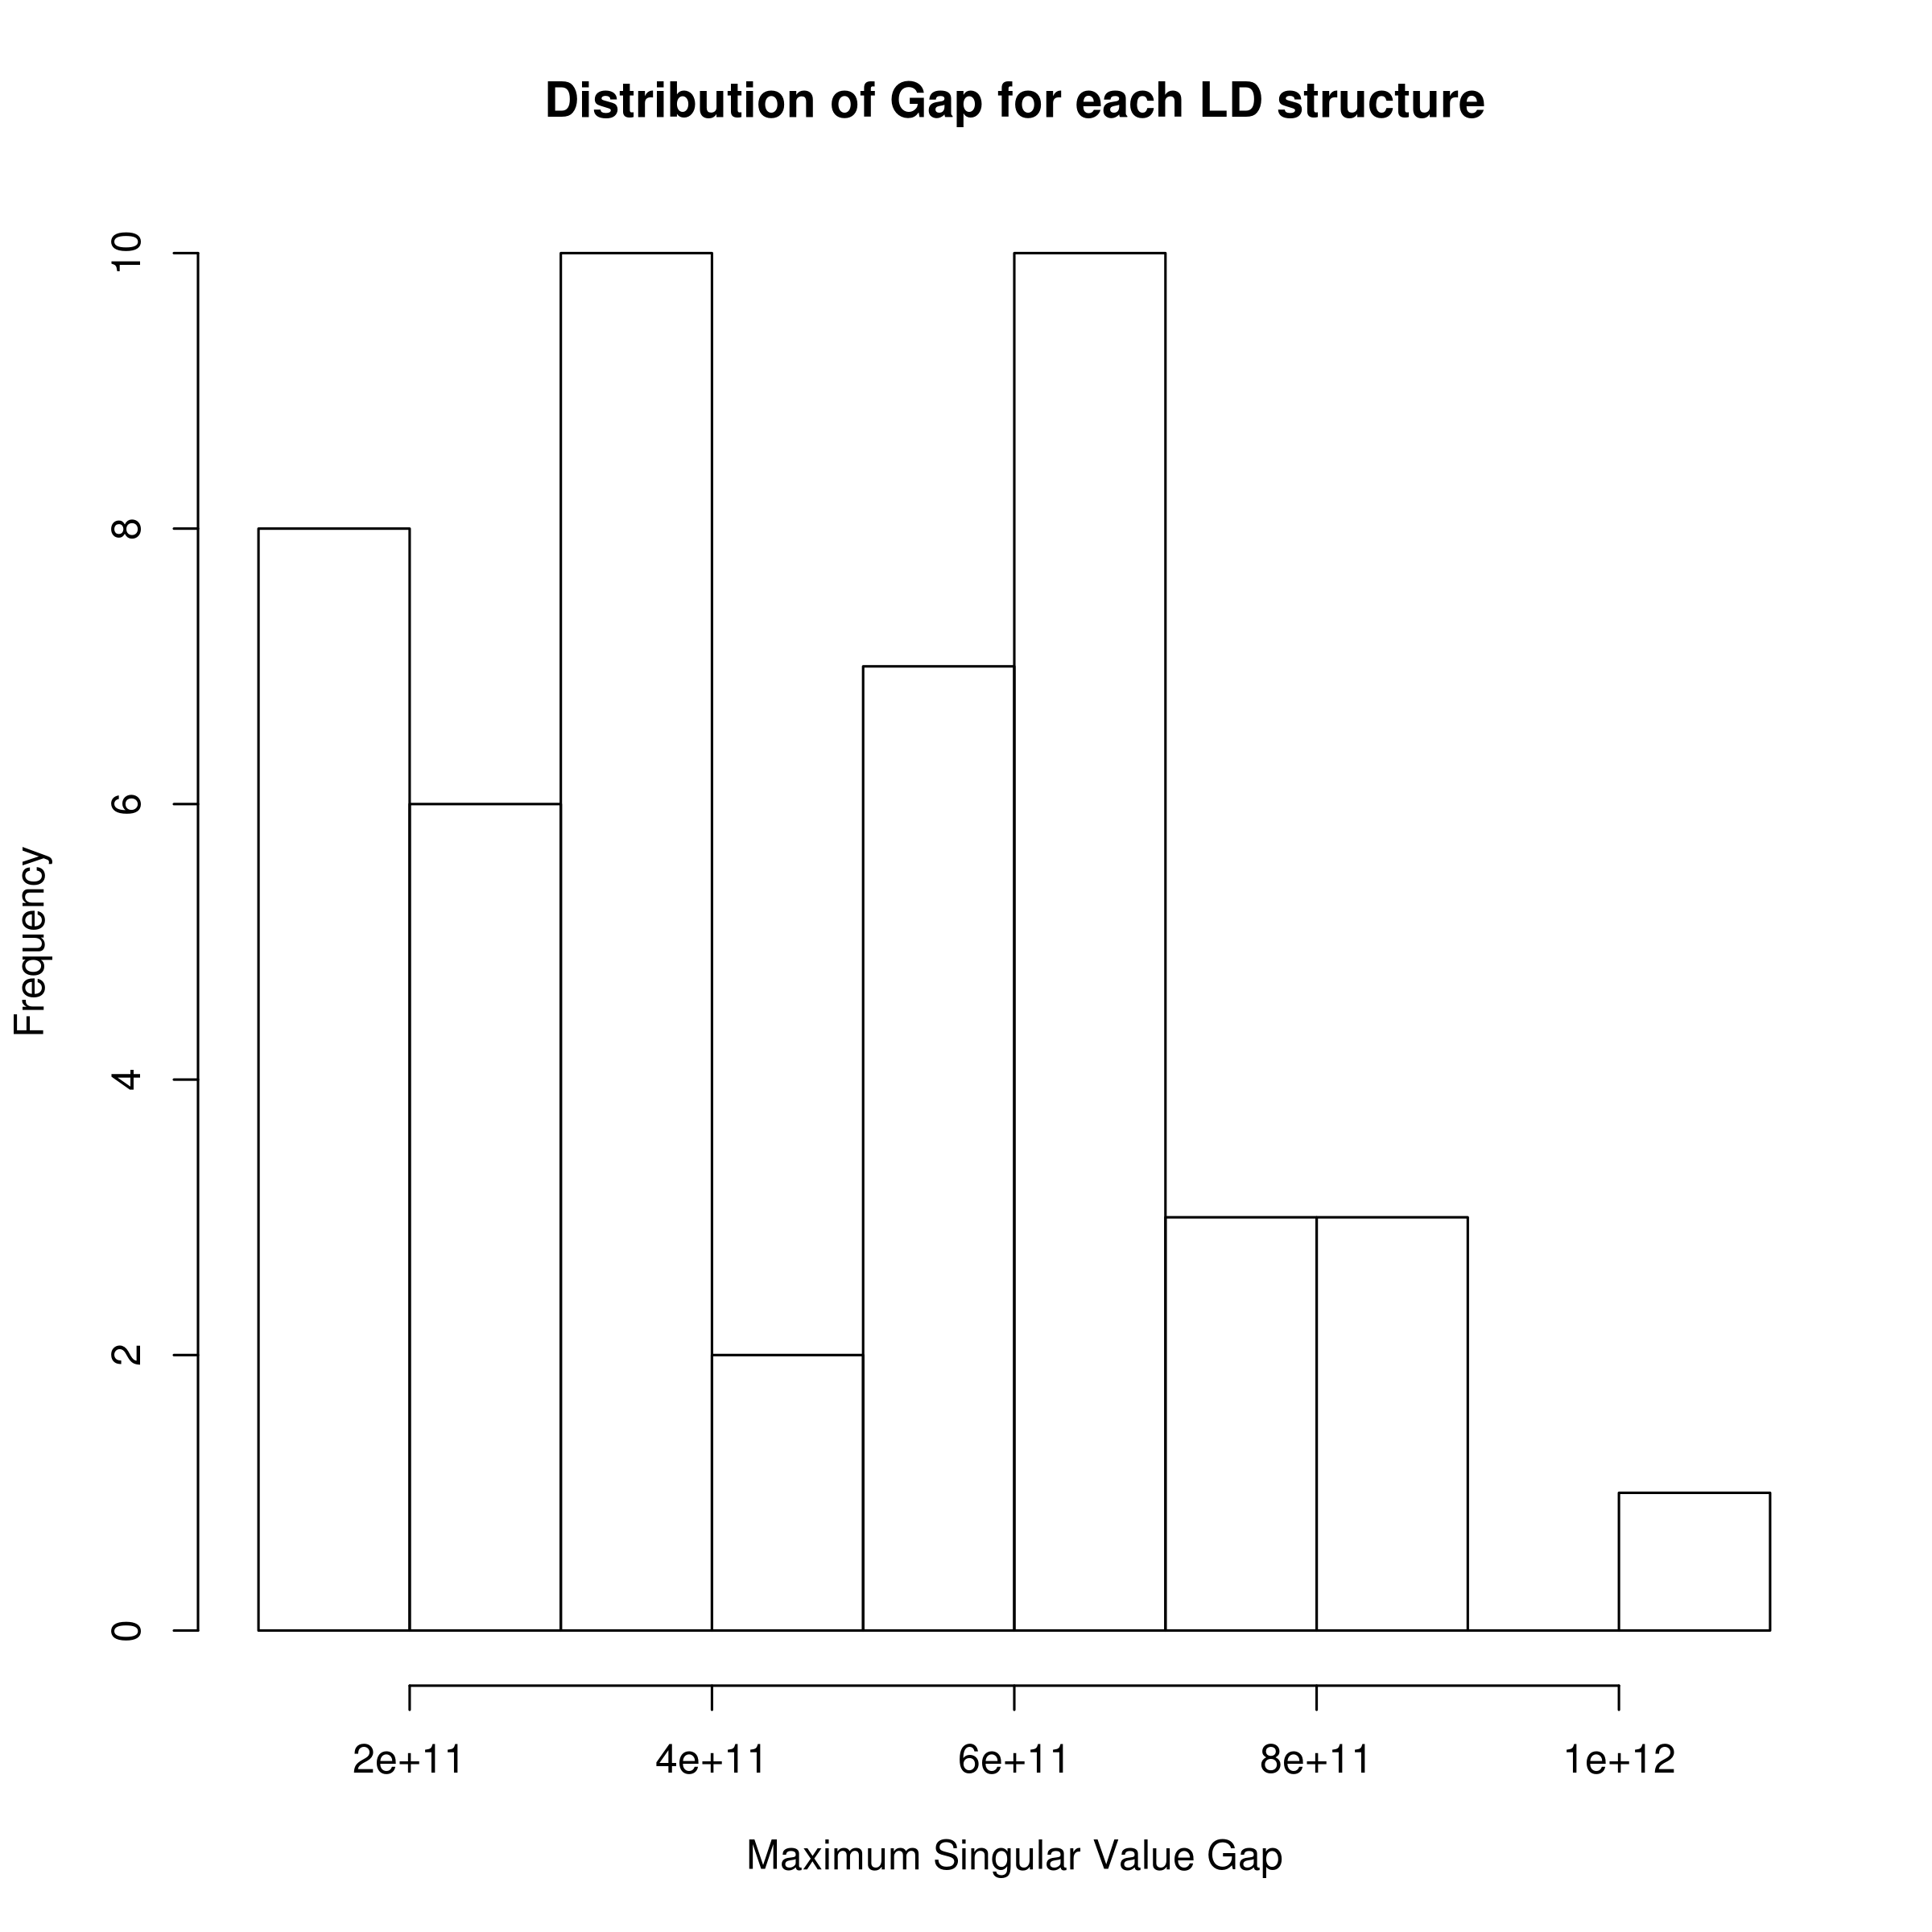
\includegraphics[width=0.5\textwidth]{figure/singular_value_distribution.png}
				\label{fig:singularValueDist}
				\vspace{-20pt}
			\end{figure}
			%\end{wrapfigure}
			
			Hence, simulation was carried out to investigate whether if \gls{LD} matrix has a well-defined rank.
			1,000 samples were randomly simulated from the HapMap \citep{Altshuler2010} \gls{CEU} population with 1,000 \glspl{SNP} randomly select from chromosome 22 using HAPGEN2 \citep{Su2011}.
			HAPGEN2 allow for the simulation of samples with \gls{LD} structure similar to that observed in the reference panel.
			The \gls{LD} matrix and its corresponding singular values were computed. 
			The whole process were repeated 50 times and the cumulative distribution of the ``gap'' of singular values were plotted (\cref{fig:singularValueDist}). 
			It is clearly shown that the \gls{LD} matrix has a well-defined rank with a mean maximum ``gap'' of 466,198,939,298.
			Therefore the choice of \gls{tSVD} for the regularization is appropriate.
			
			In view of this, \gls{tSVD} was selected as the method for regularization for solving \cref{eq:shrekEq}.
			MATLAB, NumPy and GNU Octave defined the threshold for \gls{tSVD} as $t=\epsilon\times \mathrm{max}(m,n)\times \mathrm{max}(\sigma)$ where $\epsilon$ is the machine epsilon (the smallest number a machine define as non-zero), , $n$ is the number of rows and $m$ is the number of columns. 
			Here, the same threshold definition was used in our algorithm.
			
%		\subsection{Implementation}
%			Our algorithm was implemented using C++ programming languages (version C++11) and the matrix algebra was performed using the EIGEN C++ header library \citep{eigenweb}.
%			Although the Armadillo library \citep{Sanderson2010} is faster than EIGEN \citep{Ho2011}, the speed can only be achieved when addition libraries such as OpenBLAS were installed. 
%			The use of EIGEN therefore simplify the programme installation, making it more user friendly. 
%			
%			Although \gls{tSVD} can provide an approximation to  the ill-posed \cref{eq:shrekEq}, it is an $\mathrm{O}(n^3)$ algorithm, making the computation run time prohibitive when the number of \glspl{SNP} is large.
%			Unfortunately, the number of \glspl{SNP} in a \gls{GWAS} is generally large, making it impossible to calculate the \gls{tSVD} of the whole genome. 
%			
%			From \cref{eq:svd}, it is noted that the matrix $\boldsymbol{U}$ and $\boldsymbol{V}$ are the eigenvectors of $\boldsymbol{AA}^t$ and $\boldsymbol{A}^t\boldsymbol{A}$ respectively, for any symmetric matrix such as the \gls{LD} matrix, $\boldsymbol{U}$ and $\boldsymbol{V}$ are identical. 
%			Therefore, \gls{tSVD} can be performed using eigenvalue decomposition, which is more efficient than \gls{SVD}.
%			
%			However, despite eigenvalue decomposition is more efficient than \gls{SVD}, the size of the \gls{LD} matrix is infeasible for the decomposition to be calculated. 
%			Given it is unlikely for \glspl{SNP} more than 1 \gls{mb} apart to be in \gls{LD} with each other, they are assumed to be independent of each other. 
%			\glspl{SNP} where therefore separated into 1 \gls{mb} bins where start of each bin are at least 1 \gls{mb} apart from each other. 
%			Three bins are combined to form one window, where decomposition is performed on each windows using \cref{eq:shrekEq}.
%			Only the $\boldsymbol{\hat{h^2}}$ for the bin forming the center of the window are updated.
%			We then transverse the genome with step size of 1 bin until $\boldsymbol{\hat{h^2}}$ for all bins were computed. 
%			By breaking down the genome into windows, we are able to reduce the matrix dimension,  which makes the analysis feasible.
%			Users can also choose distance other than 1 \gls{mb} as the distance between bins, allowing for a more flexible usage of the algorithm.
%			
%		\subsection{Comparing with \glsentrylong{ldsc}}
%			% main difference 
%			Conceptually, the fundamental hypothesis of \gls{ldsc} and our algorithm were quite different.
%			\gls{ldsc} were based on the ``global'' inflation of test statistic and its relationship to the \gls{LD} pattern.
%			\gls{ldsc} hypothesize that the larger the \gls{LD} score, the more likely for the \gls{SNP} to ``tag'' the causal \gls{SNP}.
%			The \gls{SNP} heritability can then be estimated through the regression between the \gls{LD} score and the summary statistic.
%			
%			On the other hand, our algorithm focuses more on the per-\gls{SNP} level.
%			Our main idea was that the individual test statistic of each \glspl{SNP} is a combination of its own effect and effect from \glspl{SNP} in \gls{LD} with it. 
%			Thus, based on this concept, our algorithm aimed to ``remove'' the inflation of test statistic introduced through the \gls{LD} between \glspl{SNP} and the heritability can be calculated by adding the test statistic of all \glspl{SNP} after ``removing'' the inflation. 
%			
%			Mathematically, the calculation of \gls{ldsc} and our algorithm were also very different. 
%			\gls{ldsc} take the sum of all $R^2$ within a 1cM region as the LD score and regress it against the test statistic to obtain the slope and intercept which represent the heritability and amount of confounding factors respectively. 
%			In their model, \gls{ldsc} assume that each \glspl{SNP} will explain the same portion of heritability
%			\begin{align}
%			 \mathrm{Var}(\beta)&=\frac{h^2}{M}\boldsymbol{I}\\
%			 M &= \text{number of SNPs}\notag\\
%			 \beta &= \text{vector containing per normalized genotype effect sizes}\notag\\
%			 I &= \text{identity matrix}\notag\\
%			 h^2 &= \text{heritability}\notag
%			\end{align}
%			
%			As for our algorithm, the whole \gls{LD} matrix were used and inverted to decompose the \gls{LD} from the test statistic. 
%			There were no assumption of the amount of heritability explained by each \glspl{SNP}. 
%			However, our algorithm does assumed that the mean of the $\chi^2$ test statistic to be one (e.g. no inflation in the summary statistics), thus our estimation might inflates shall there be any confounding factors in the \gls{GWAS} summary statistics.
%			
	\subsection{Comparing Different LD correction Algorithms}
		\label{sec:ldSim}
		% Might want to remove this section as we no longer use this correction
		An important consideration in our algorithm is the sampling error in \gls{LD}.
		In reality, the population \gls{LD} matrix is not available.
		Therefore , the \gls{LD} matrix must be estimated from various reference panels such as the 1000 genome project \citep{Project2012} or the HapMap project \citep{Altshuler2010}.
		Given these reference panels are subsets of the whole population, this results in sampling errors in the estimated sample \gls{LD}.
		The sample \gls{LD} can then be represented as:
		$$
		\hat{R} = R+\epsilon
		$$
		where $R$ is the population \gls{LD} and $\epsilon$ is the sampling error which is unbiased.
		However, in \cref{eq:fullShrek}, squared \gls{LD} are required.
		The expected value of the \gls{LD} squared ($R^2$) is then calculated as
		\begin{align}
		\mathrm{\hat{R^2}} &= \mathrm{E}[(R+\epsilon)^2] \notag\\
		&=\mathrm{E}(R^2+2R\epsilon+\epsilon^2) \notag\\
		&=\mathrm{E}(R^2)+\mathrm{E}(\epsilon^2)
		\end{align}
		A positive bias is observed in the sample $R^2$.
		
		\citet{Weir1980,Wang2007} proposed methods for the correction of sample $R^2$:
		\begin{align}
		\text{Ezekiel}: \tilde{R^2}&= 1-\frac{n-1}{n-2}(1-\hat{R^2})\label{eq:ezekiel} \\
		\text{Olkin-Pratt}: \tilde{R^2}&=1-\frac{(n-3)(1-\hat{R^2})}{n-2}(1+\frac{2(1-\hat{R^2})}{n})\label{eq:okin} \\
		\text{Pratt}: \tilde{R^2}&=1-\frac{(n-3)(1-\hat{R^2})}{n-2}(1+\frac{2(1-\hat{R^2})}{n-3.3})\label{eq:pratt} \\
		\text{Smith}: \tilde{R^2}&=1-\frac{n}{n-1}(1-\hat{R^2}) \label{eq:smith}\\
		\text{Weir}: \tilde{R^2}&=\hat{R^2}-\frac{1}{2n} \label{eq:weir}
		\end{align}
		where $n$ is the number of samples used to calculate the $R^2$ and $\tilde{R^2}$ is the corrected $R^2$.
		
		Again, simulations were performed to assess the performance of each individual correction methods.
		Firstly, 5,000 \glspl{SNP} with \gls{maf} $\ge0.1$ were randomly selected from chromosome 22 from the 1000 genome \gls{CEU} haplotypes and were used as an input to HAPGEN2 \citep{Su2011} to simulate 1,000 individuals.
		HAPGEN2 is a simulation tools which simulates new haplotypes as an imperfect mosaic of haplotpyes from a reference panel and the haplotypes that have already been simulated using the \textit{Li and Stephens} (LS) model of \gls{LD} \citep{Li2003}.
		This allows for the simulation of genotypes with \gls{LD} structures comparable to those observed in \gls{CEU} population. 
		Of those 5,000 \glspl{SNP}, 100 of them were randomly selected as the causal variants. 
		\citet{Orr1998} suggested that the exponential distribution could be used to approximate the genetic architecture of adaptation. 
		As a result, effect sizes were simulated with an exponential distribution with $\lambda=1$:
		\begin{align}
		\theta&=\mathrm{exp}(\lambda=1)\notag\\
		\beta&=\pm\sqrt{\frac{\theta \times h^2}{\sum \theta}}
		\label{eq:randomEffect}
		\end{align}
		with a random direction of effect.
		The simulated effects were then randomly distributed to each causal \glspl{SNP}.
			
		Using the normalized genotype matrix of the causal \glspl{SNP} of all individuals ($\boldsymbol{X}$) and the vector of effect sizes ($\boldsymbol{\beta}$), the phenotype were simulated with heritability of $h^2$ using
		\begin{align}
		\epsilon_i&\sim N(0,\mathrm{Var}(\boldsymbol{X\beta})\frac{1-h^2}{h^2} )\notag\\
		\boldsymbol{\epsilon} &= (\epsilon_1,\epsilon_2,...,\epsilon_n)^t\notag\\
		\boldsymbol{y} &= \boldsymbol{X\beta}+\boldsymbol{\epsilon}
		\label{eq:simulationOfPhenotype}
		\end{align}
		
		To simulate the whole spectrum of heritability, the $h^2$ were varied from 0 to 0.9 with increment of 0.1.
		
		The association between the genotype and phenotype were then calculated using PLINK \citep{Purcell2007}.
		Heritability estimation were then performed based on the resulting summary statistics using different \gls{LD} correction algorithms.
		An independent 500 samples, which corresponds to the average sample size of each super population form the 1,000 genome project, were simulated as a reference panel for the calculation of \gls{LD} matrix.
		This is because in reality, the raw sample genotypes were unavailable and has to rely on an independent reference panel for the calculation of \gls{LD} matrix. 
		Thus, this simulation procedure should provide a realistic representation of the common usage of the algorithm.
		
		The whole process was repeated 50 times such that a distribution of the estimates can be obtained. 
		In summary, the following simulation procedure was performed:
		\begin{enumerate}
			\item Randomly select 5,000 \glspl{SNP} with \gls{maf}$>0.1$ from chromosome 22
			\item Simulate 500 samples using HAPGEN2 and used as the reference panel
			\item Randomly generate 100 effect sizes with \cref{eq:randomEffect}
			\item Randomly assign the effect sizes to 100 \glspl{SNP} with heritability from 0 to 0.9 (increment of 0.1)
			\item Simulate 1,000 samples using HAPGEN2 and calculate their phenotype according to \cref{eq:simulationOfPhenotype} 
			\item Perform heritability estimation using our algorithm with different \gls{LD} correction algorithm
			\item Repeat step 5-6 50 times
		\end{enumerate}
		
		\subsection{Comparison with Other Algorithms}
		After identifying the optimal \gls{LD} correction algorithm, it is important to compare the performance of our algorithm to the other existing methods.
		Therefore, simulations were performed where quantitative and binary traits were simulated under different genetic architectures. 
		The effect of sampling strategies, such as random sampling and extreme phenotype selection, on the heritability estimation were also investigated.
		
		Currently, the only other algorithm that utilizes the \gls{GWAS} summary statistics to \gls{SNP}-heritability is the \gls{ldsc} \citep{Bulik-Sullivan2015}.
		Whereas \gls{gcta} \citep{Yang2011} is the most commonly used programme for the estimation of \gls{SNP}-heritability from \gls{GWAS} data when the raw genotypes are available. 
		Therefore, the performance of our algorithm was compared to \gls{ldsc} and \gls{gcta}.
		As no confounding factors were simulated, the intercept estimation function in \gls{ldsc} will be penalized with a larger \gls{se}. 
		Thus, performance of \gls{ldsc} with fixed intercept (-{}-no-intercept) were also inspected to avoid bias against \gls{ldsc}.
		
		\subsubsection{Sample Size}
			The sample size is the most important parameter in determining the \gls{se} of the estimates. 
			As sample size increases, the samples will be more representative of the true population and will provide a more accurate estimation of the parameters, therefore resulting in a smaller \gls{se}.
			% awk -F "\t" '{print $2"\t"$9}' full | uniq | sed -e 's/[^0-9[:space:]]//g' | awk '{for(i=2;i<=NF;++i)j+=$i; print $1" "j; j=0}' | sort | uniq  %script for text mining
			Using simple text mining, the sample size distribution of \gls{GWAS} was obtained from the \gls{GWAS} catalog \citep{Welter2014}.
			The average sample size was 7,874, with a median count of 2,506 and a lower quartile at 940. 
			We argued that if the algorithms performed well with a small sample size (e.g. 1,000 samples), their performance should improve as sample size increases.
			Thus, to reduce the computation time required for the simulation, only 1,000 samples were simulated in each simulations unless otherwise stated.
				
%			\begin{wrapfigure}{R}{8cm}
%				\centering
%				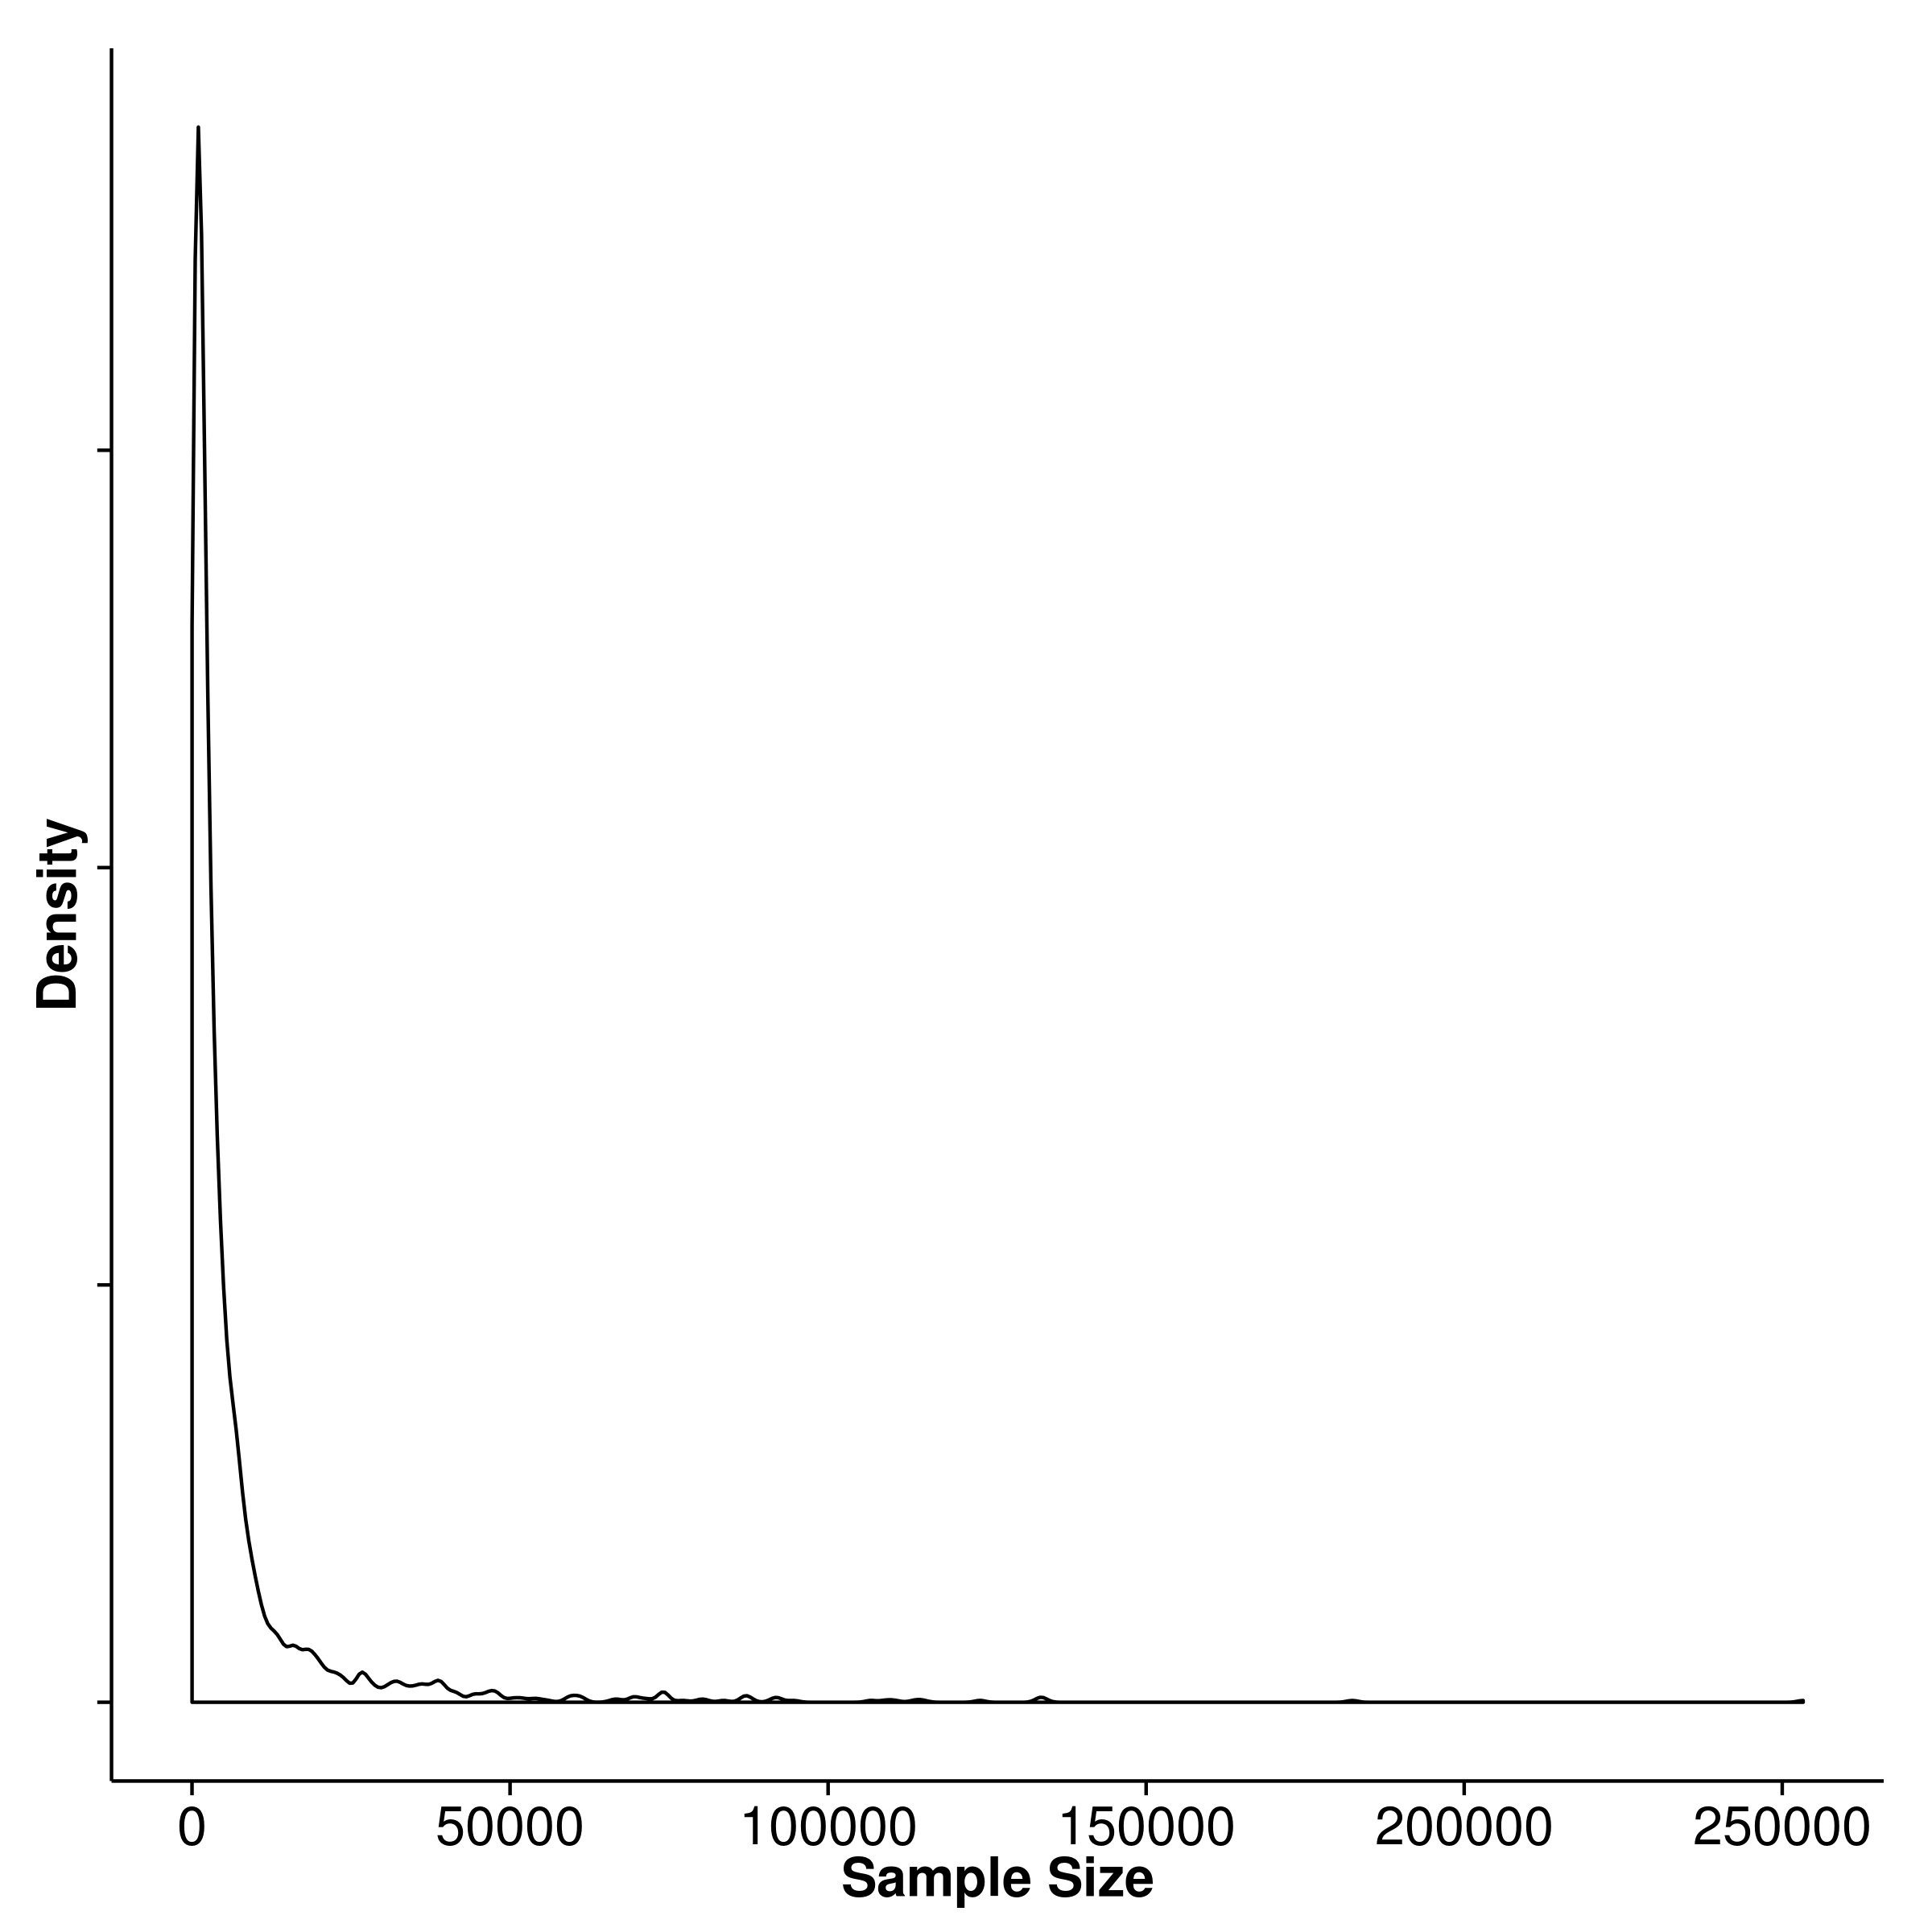
\includegraphics[width=0.5\textwidth]{figure/gwasSampleSize.png}
%				\caption[GWAS Sample Size distribution]{
%					\gls{GWAS} sample size distribution.
%				}
%				\label{fig:gwasCata}
%			\end{wrapfigure}
%			
		\subsubsection{Number of SNPs in Simulation}
			To reduce the computational cost for simulation, only 50,000 \glspl{SNP} from chromosome 1 were used for simulation, which correspond to 200 \glspl{SNP} within a 1 \gls{mb} region.
			
		\subsubsection{Genetic Architecture}
			The number of causal \glspl{SNP}, the effect size of the causal \glspl{SNP} and the heritability of the trait are all important factors contributing to the genetic architecture of a trait. 
		
			First and foremost, in order to investigate the performance of the \gls{SNP} heritability estimation algorithms, traits with different heritability have to be considered.
			Therefore, traits with heritability ranging from 0 to 0.9 with increment of 0.1 were simulated. 
		
%			Secondly, in real life scenario, the ``causal'' variant might not be readily included on the \gls{GWAS} chip and are only ``tagged'' by \glspl{SNP} included on the \gls{GWAS} chip.
%			However, to simplify our simulation, all ``causal'' variants were included in our simulation (e.g. perfectly ``tagged'').

			Secondly, to obtain a realistic \gls{LD} pattern, genotypes were simulated using the HAPGEN2 programme \citep{Su2011}, using the 1000 genome \gls{CEU} haplotypes as an input.
			As \gls{GWAS} usually lack power in detecting rare variants (e.g. \gls{maf} $<$ 0.05), \glspl{SNP} with \gls{maf} $<0.05$ were excluded.
			
			Thirdly, to investigate the performance of the algorithms with a different number of causal \glspl{SNP} ($k$), the number of causal \glspl{SNP} were varied with $k\in\{5, 10, 50, 100, 500\}$.
			The effect sizes were then simulated using \cref{eq:randomEffect} and the phenotype were simulated using \cref{eq:simulationOfPhenotype}.
			
			For \gls{gcta}, the sample genotypes were provided to calculate the genetic relationship matrix. 
			Sample phenotypes were also provided for \gls{gcta} to estimate the \gls{SNP} heritability.
			
			On the other hand, for \gls{ldsc} and our algorithm, an independent 500 samples were simulated as the reference panel for the calculation of \gls{LD} scores and \gls{LD} matrix. 
			The association between the genotype and phenotype were calculated using PLINK \citep{Purcell2007}.
			The summary statistics and the reference panel were then provided for \gls{ldsc} and our algorithm to estimate the \gls{SNP} heritability.
			This simulation procedure should provide a realistic representation of the common usage of the algorithms.
			
			For each population, the whole process was repeated 50 times such that a distribution of the estimate can be obtained. 
			In total, 10 independent populations were simulated.
			In summary, the simulation follows the following procedures:
			\begin{enumerate}
				\item Randomly select 50,000 \glspl{SNP} with \gls{maf}$>0.05$ from chromosome 1
				\item Simulate 500 samples using HAPGEN2 to be served as a reference panel
				\item Randomly generate $k$ effect size with $k \in \{5,10,50,100,500\}$ following \cref{eq:randomEffect}, with heritability ranging from 0 to 0.9 (increment of 0.1)
				\item Randomly assign the effect size to $k$ \glspl{SNP}
				\item Simulate 1,000 samples using HAPGEN2 and calculate their phenotype according to \cref{eq:simulationOfPhenotype}
				\item Perform heritability estimation using our algorithm, \gls{gcta}, \gls{ldsc} with fixed intercept and \gls{ldsc} with intercept estimation.
				\item Repeat step 5-6 50 times
				\item Repeat step 1-7 10 times
			\end{enumerate}
		
		\subsubsection{Extreme Effect Size}
		\label{sec:extremeEffectSim}
		It is possible for a trait to have \glspl{SNP} that account for a larger portion of the heritability.
		For example, the deleterious mutations on \textit{RET} account for $\approx50\%$ of the familial cases of the Hirschsprung's disease yet some of the heritability was still missing.
		\citet{Gui2013} therefore suggested that there might be more variants with small effects that have not been identified.
		
		To simulate extreme effect size, 100 causal \glspl{SNP} were simulated where $m$ of those account for 50\% of all the effect sizes with $m\in\{1,5,10\}$.
		The effect sizes were then calculated as
		\begin{align}
		\beta_{eL} &= \pm\sqrt{\frac{0.5h^2}{m}} \notag\\
		\beta_{eS} &= \pm\sqrt{\frac{0.5h^2}{100-m}} \notag\\
		\beta &= \{\beta_{eL}, \beta_{eS}\}
		\label{eq:extremEffect}
		\end{align}
		The effect sizes were then randomly assigned to 100 causal \glspl{SNP} and phenotypes were calculated using \cref{eq:simulationOfPhenotype}.
		The following simulation procedure were then performed:
		\begin{enumerate}
			\item Randomly select 50,000 \glspl{SNP} with \gls{maf} $>0.05$ from chromosome 1
			\item Simulate 500 samples using HAPGEN2 and used as the reference panel
			\item Randomly generate 100 effect size where $m$ has extreme effect, following \cref{eq:extremEffect}, with $m\in\{1,5,10\}$
			\item Randomly assign the effect size to 100 \glspl{SNP}
			\item Simulate 1,000 samples using HAPGEN2 and calculate their phenotype according to \cref{eq:simulationOfPhenotype}
			\item Perform heritability estimation using our algorithm, \gls{ldsc} with fixed intercept, \gls{ldsc} with intercept estimation and \gls{gcta}
			\item Repeat step 5-6 50 times
			\item Repeat step 1-7 10 times
		\end{enumerate}
		
		\subsubsection{Case Control Studies}
		In the simulation of case control samples, two additional parameters, the population prevalence ($p$) and observer prevalence ($q$), have to be taken into consideration. 
		The liability threshold model were used to model the samples.
		In order to simulate a trait with population prevalence of $p$ and observed prevalence of $q$ with $n$ cases, $\min(\frac{n}{p}, \frac{n}{q})$ samples were required to be simulated. 
		For example, if the observed prevalence is $50\%$ with the population prevalence of $1\%$, a minimum of 100,000 needs to be simulated in order to obtain 1,000 cases.
		
		Therefore when the population prevalence is small, a tremendous amount of computational resources are required in order to perform the simulation.
		To reduce the burden of computation, the observed prevalence was limited to 50\% and only 5,000 \glspl{SNP} were simulated from chromosome 22.
		By changing from chromosome 1 to chromosome 22, the number of \glspl{SNP} simulated can be reduced without significantly reducing the \gls{SNP} density.
		
		To investigate the effect of population prevalence and the heritability of the traits to the performance of the algorithms, different population prevalence ($p$) were simulated with $p\in\{0.5, 0.1, 0.05, 0.01\}$.
		The heritability of the trait were also varied from 0 to 0.9 with increment of 0.1.

		In brief, 5,000 \glspl{SNP} with \gls{maf} $>0.05$ were randomly selected from chromosome 22 as an input to HAPGEN2. 
		$k$ causal \glspl{SNP} with $k\in\{10,50,100,500\}$ were randomly selected, each with effect sizes simulated based on \cref{eq:randomEffect}.
		$\frac{1,000}{p}$ samples were then simulated and their phenotype were calculated using \cref{eq:simulationOfPhenotype}.
		The phenotypes were then standardized and cases were defined as sample with phenotype passing the liability threshold with respect to $p$.
		An equal amount of controls were then randomly selected from samples with phenotype below the liability threshold.
			
		In summary, the case control simulation follows:
		\begin{enumerate}
			\item Randomly select 5,000 \glspl{SNP} with \gls{maf}$>0.05$ from chromosome 22
			\item Simulate 500 samples using HAPGEN2 and used as a reference panel
			\item Randomly generate $k$ effect size following \cref{eq:randomEffect} where $k\in\{10,50,100,500\}$
			\item Randomly assign the effect size to $k$ \glspl{SNP}
			\item Simulate $\frac{1,000}{p}$ samples using HAPGEN2 and calculate their phenotype according to \cref{eq:simulationOfPhenotype}
			\item Define case control status using the liability threshold and randomly select the same number of case and controls for statistic analysis
			\item Perform heritability estimation using our algorithm, \gls{ldsc} with fixed intercept, \gls{ldsc} with intercept estimation and \gls{gcta}
			\item Repeat step 5-7 50 times
			\item Repeat step 1-8 10 times
		\end{enumerate}
		
		\subsubsection{Extreme Phenotype Sampling}
		Simulation was performed to investigate the effect of extreme phenotype sampling on the performance of the algorithms.
		50,000 \glspl{SNP} with \gls{maf} $>0.05$ were selected from chromosome 1 and were used as an input for HAPGEN2.
		Again, 500 samples were first simulated to serve as the reference panel for \gls{ldsc} and our algorithm.
		
		From the 50,000 \glspl{SNP}, 100 \glspl{SNP} were randomly selected as the causal \glspl{SNP} and their effect sizes were simulated using \cref{eq:randomEffect}.
		Two settings are considered: sampling 10\% high and 10\% low extreme phenotypes ($K=0.1$); sampling 20\% high and 20\% low extreme phenotypes ($K=0.2$).
		A total of $\frac{500}{K}$ samples were simulated where the sample phenotypes were calculated using \cref{eq:simulationOfPhenotype}.
		Phenotypes were then standardized and 500 samples from each extreme ends of the phenotype distribution such that a total of 1,000 samples were obtained. 
		To compare the effect of extreme phenotype sampling and random sampling strategies on the performance of the algorithms, 1,000 samples were randomly drawn from all samples.
		
		As the extreme phenotype sampling were not natively supported by the \gls{ldsc} and \gls{gcta}.
		To allow for a fair comparison, extreme phenotype adjustment from \citet{Sham2014} were applied to the estimates from \gls{ldsc} and \gls{gcta}.
		Finally, the heritability estimated based on different sampling strategies were compared.
		For each population, the whole process were repeated 50 times. 
		In total, 10 independent populations were simulated. 
		In summary, the following simulation procedures were used:
		\begin{enumerate}
			\item Randomly select 50,000 \glspl{SNP} with \gls{maf}$>0.05$ from chromosome 1
			\item Simulate 500 samples using HAPGEN2 and used as the reference panel
			\item Randomly generate 100 effect size following \cref{eq:randomEffect}, with heritability ranging from 0 to 0.9 (increment of 0.1)
			\item Randomly assign the effect sizes to 100 \glspl{SNP}
			\item Simulate $\frac{500}{K}$ samples using HAPGEN2 where $K$ is the portion of samples selected from the extreme end of the distribution with $K\in\{0.1,0.2\}$
			\item Phenotype of the samples were calculated according to \cref{eq:simulationOfPhenotype} and were standardized
			\item Top 500 and bottom 500 samples (ranked by phenotype) were selected, representing the extreme phenotype sample selection strategy
			\item 1,000 samples were also randomly selected to represent the general random sampling strategy
			\item Perform heritability estimation using our algorithm, \gls{gcta}, \gls{ldsc} with fixed intercept and \gls{ldsc} with intercept estimation.
			\item Adjust the estimation from \gls{ldsc} and \gls{gcta} by the extreme phenotype adjustment factor as proposed by \citet{Sham2014}
			\item Repeat step 5-10 50 times
			\item Repeat step 1-11 10 times
		\end{enumerate}
		
		
%	\section{Simulation with Real Data}
	% Reason of not simulated with real data = variance
%	Although HAPGEN2 helps us to simulate realistic samples, it is also important for us to test the performance of the algorithms in real data. 
%	To performing simulations on real data, we used the 2,025 Han Chinese control samples obtained form \citet{Wong2014} for the simulation.
%	The genomic coordinates were first converted to hg19 using liftover \citep{Hinrichs2006} such that it is compatible with the reference genome.
%	As the samples were mostly originated from southern China, we used the southern Chinese (CHS) samples from the 1000 genome project \citep{Project2012} as the reference panel.
	
%	By assuming there is no \gls{LD} for \glspl{SNP} located on different chromosomes, we only perform the simulation of chromosome 22. 
%	From chromosome 22, we first randomly select $k$ \glspl{SNP} with $k\in\{5,10,50,100,500\}$ as causal \glspl{SNP} and randomly select effect size using \cref{eq:randomEffect}.
%	Again, we would like to investigate the performance of the tools with traits of different heritability thus we varies $h^2$ from $0$ to $0.9$ with increment of $0.1$.
%	Then the phenotype of each individuals were simulated based on \cref{eq:simulationOfPhenotype}.
%	From the 2,025 samples, we randomly select 1,000 samples for the estimation of heritability.
%	For each sets of causal \glspl{SNP} we repeats the analysis 50 times, then we randomly draw a different set of causal \glspl{SNP} and repeat the whole process 10 times. 
%	To summarize
%	\begin{enumerate}
%		\item Extract \glspl{SNP} from chromosome 22 from data of \citet{Wong2014}
%		\item Liftover the coordinates to hg19
%		\item Randomly generate $k$ effect sizes and assign them to $k$ random \glspl{SNP}, with $k\in\{5,10,50,100,500\}$
%		\item Simulate the phenotype using \cref{eq:simulationOfPhenotype}
%		\item 1,000 samples were randomly selected for subsequent analysis
%		\item Perform heritability estimation using our algorithm, \gls{gcta}, \gls{ldsc} with fixed intercept and \gls{ldsc} with intercept estimation.
%		\item Repeat step 5-6 50 times
%		\item Repeat step 3-7 10 times
%	\end{enumerate}
	
	\subsection{Application to Real Data}
	\label{sec:realData}
	To demonstrate our algorithm also works outside of simulated data, we also estimated the heritability of \glng{scz} and other psychiatric disorders using the \gls{pgc} datasets \citep{Ripke2014,PsychiatricGWASConsortiumBipolarDisorderWorkingGroup2011,Ripke2013b}.
	\gls{ldsc} were used alongside our algorithm to serves as a baseline comparison.
	
	The reference genome were downloaded from 1000 genome (hg19) \citep{Project2012} and were converted to PLINK binaries using the PLINK -{}-vcf function. 
	The European super population was extracted which contains a total of 503 samples.
	Singleton and multi-allelic \glspl{SNP} were filtered out from the reference panel.	
	Cryptic relatedness between samples can inflate the \gls{LD} due to increased allele sharing amongst relatives. 
	It is therefore important to filter out related samples.
	Genotypes were first pruned, then the \gls{ibd} between samples were calculate using the PLINK option -{}-genome.
	Sample pairs with relatedness $\ge 0.125$ ($\approx$ third degree relatedness) were removed.
	In total, 446 samples remained after quality control.
	The \gls{LD} score was calculated based on the 446 samples using a 1 \gls{mb} window size.
	\glspl{SNP} with \gls{maf} $<0.1$ were filtered out by default.
	\gls{ldsc} analysis were then performed with and without the intercept estimation (-{}-no-intercept) to serve as a baseline comparison.
	
	The summary statistics were obtained from the \gls{pgc} website. 
	As \glspl{SNP} in the bipolar and major depression data follows the old genomic annotations (hg18), liftover \citep{Hinrichs2006} were performed to convert the genomic coordinates to genome version hg19.
	Due to difference in composition of the sex chromosome in male and female (e.g. XY in male, XX in female) and the lack of information on the male to female ratio, it is difficult to estimate the \glspl{SNP} heritability on the sex chromosomes.
	Special care are required for the estimation of \gls{SNP} heritability on the sex chromosome and this function has not been implemented in either \gls{shrek} or \gls{ldsc}.
	Therefore, the \gls{SNP} heritability were only estimated using the autosomal \glspl{SNP}.
	Furthermore, the \gls{mhc} region (chr6:25,000,000-35,000,000) was removed from the analysis due to its unusual \gls{LD} and genetic architecture \citep{Bulik-Sullivan2015}.
	
	
	As the datasets contain binary traits, the population prevalence of the trait has to be provided in order for the adjustment of the ascertainment bias. 
	Based on \citet{Bulik-Sullivan2015} a population prevalence of 0.15 were selected for major depression disorder and 0.01 were selected for \glng{scz} and bipolar disorder.
	
	Unfortunately, because of the high \gls{SNP} density of the \gls{pgc} \glng{scz} \gls{GWAS}, the computational resources required to complete the \gls{SNP} heritability estimation exceeds the current available resources.
	To facilitate the analysis, the distance between each bin was reduced to 50,000 \gls{bp} for our algorithm.
	This will results in an inflation in the final estimates.
	Therefore estimates from our algorithm can only serve as an upper bound of the true \gls{SNP} heritability.
	
	\section{Results}
		The heritability estimation were implemented in \gls{shrek} and is available on \url{https://github.com/choishingwan/shrek}.  
		\subsection{LD Correction}
		\begin{figure}
			\centering
			\subfloat[Mean Estimation]{
				\scalebox{.4}{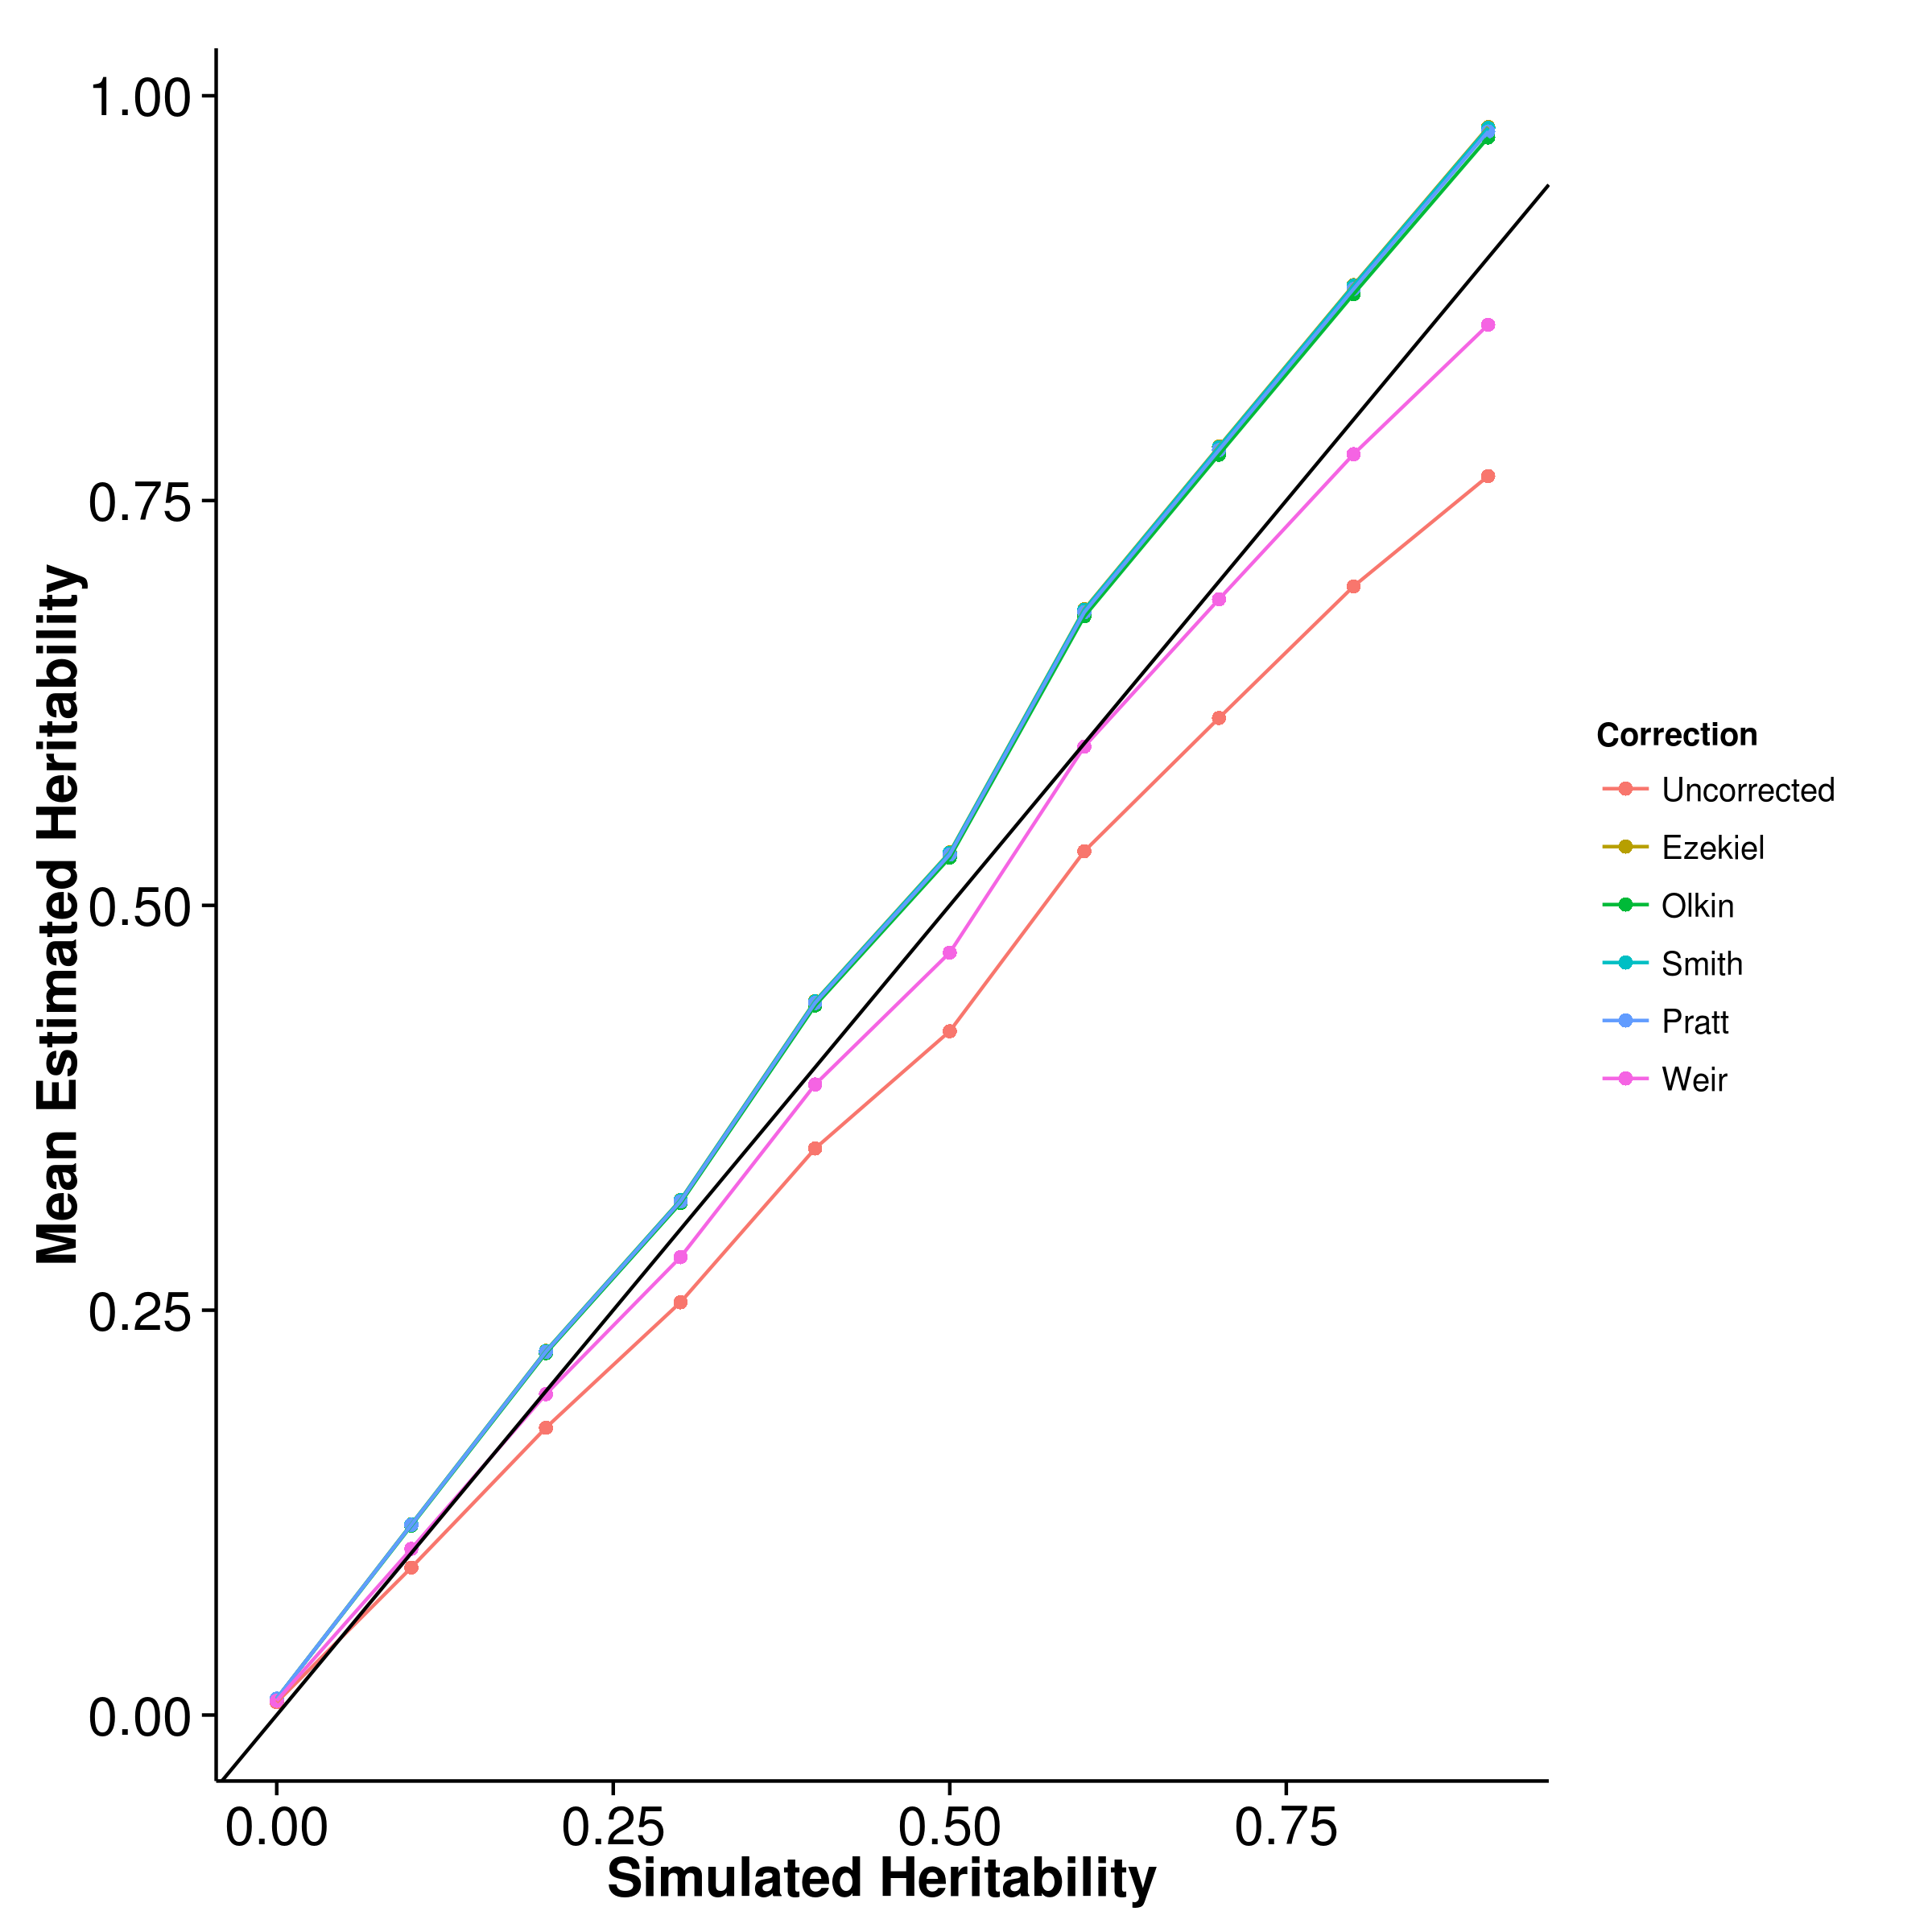
\includegraphics{figure/quantitative/ld_correct/ldCom_mean.png}}
				\label{fig:meanLDCor}
			}
			\subfloat[Empirical Variance]{
				\scalebox{.4}{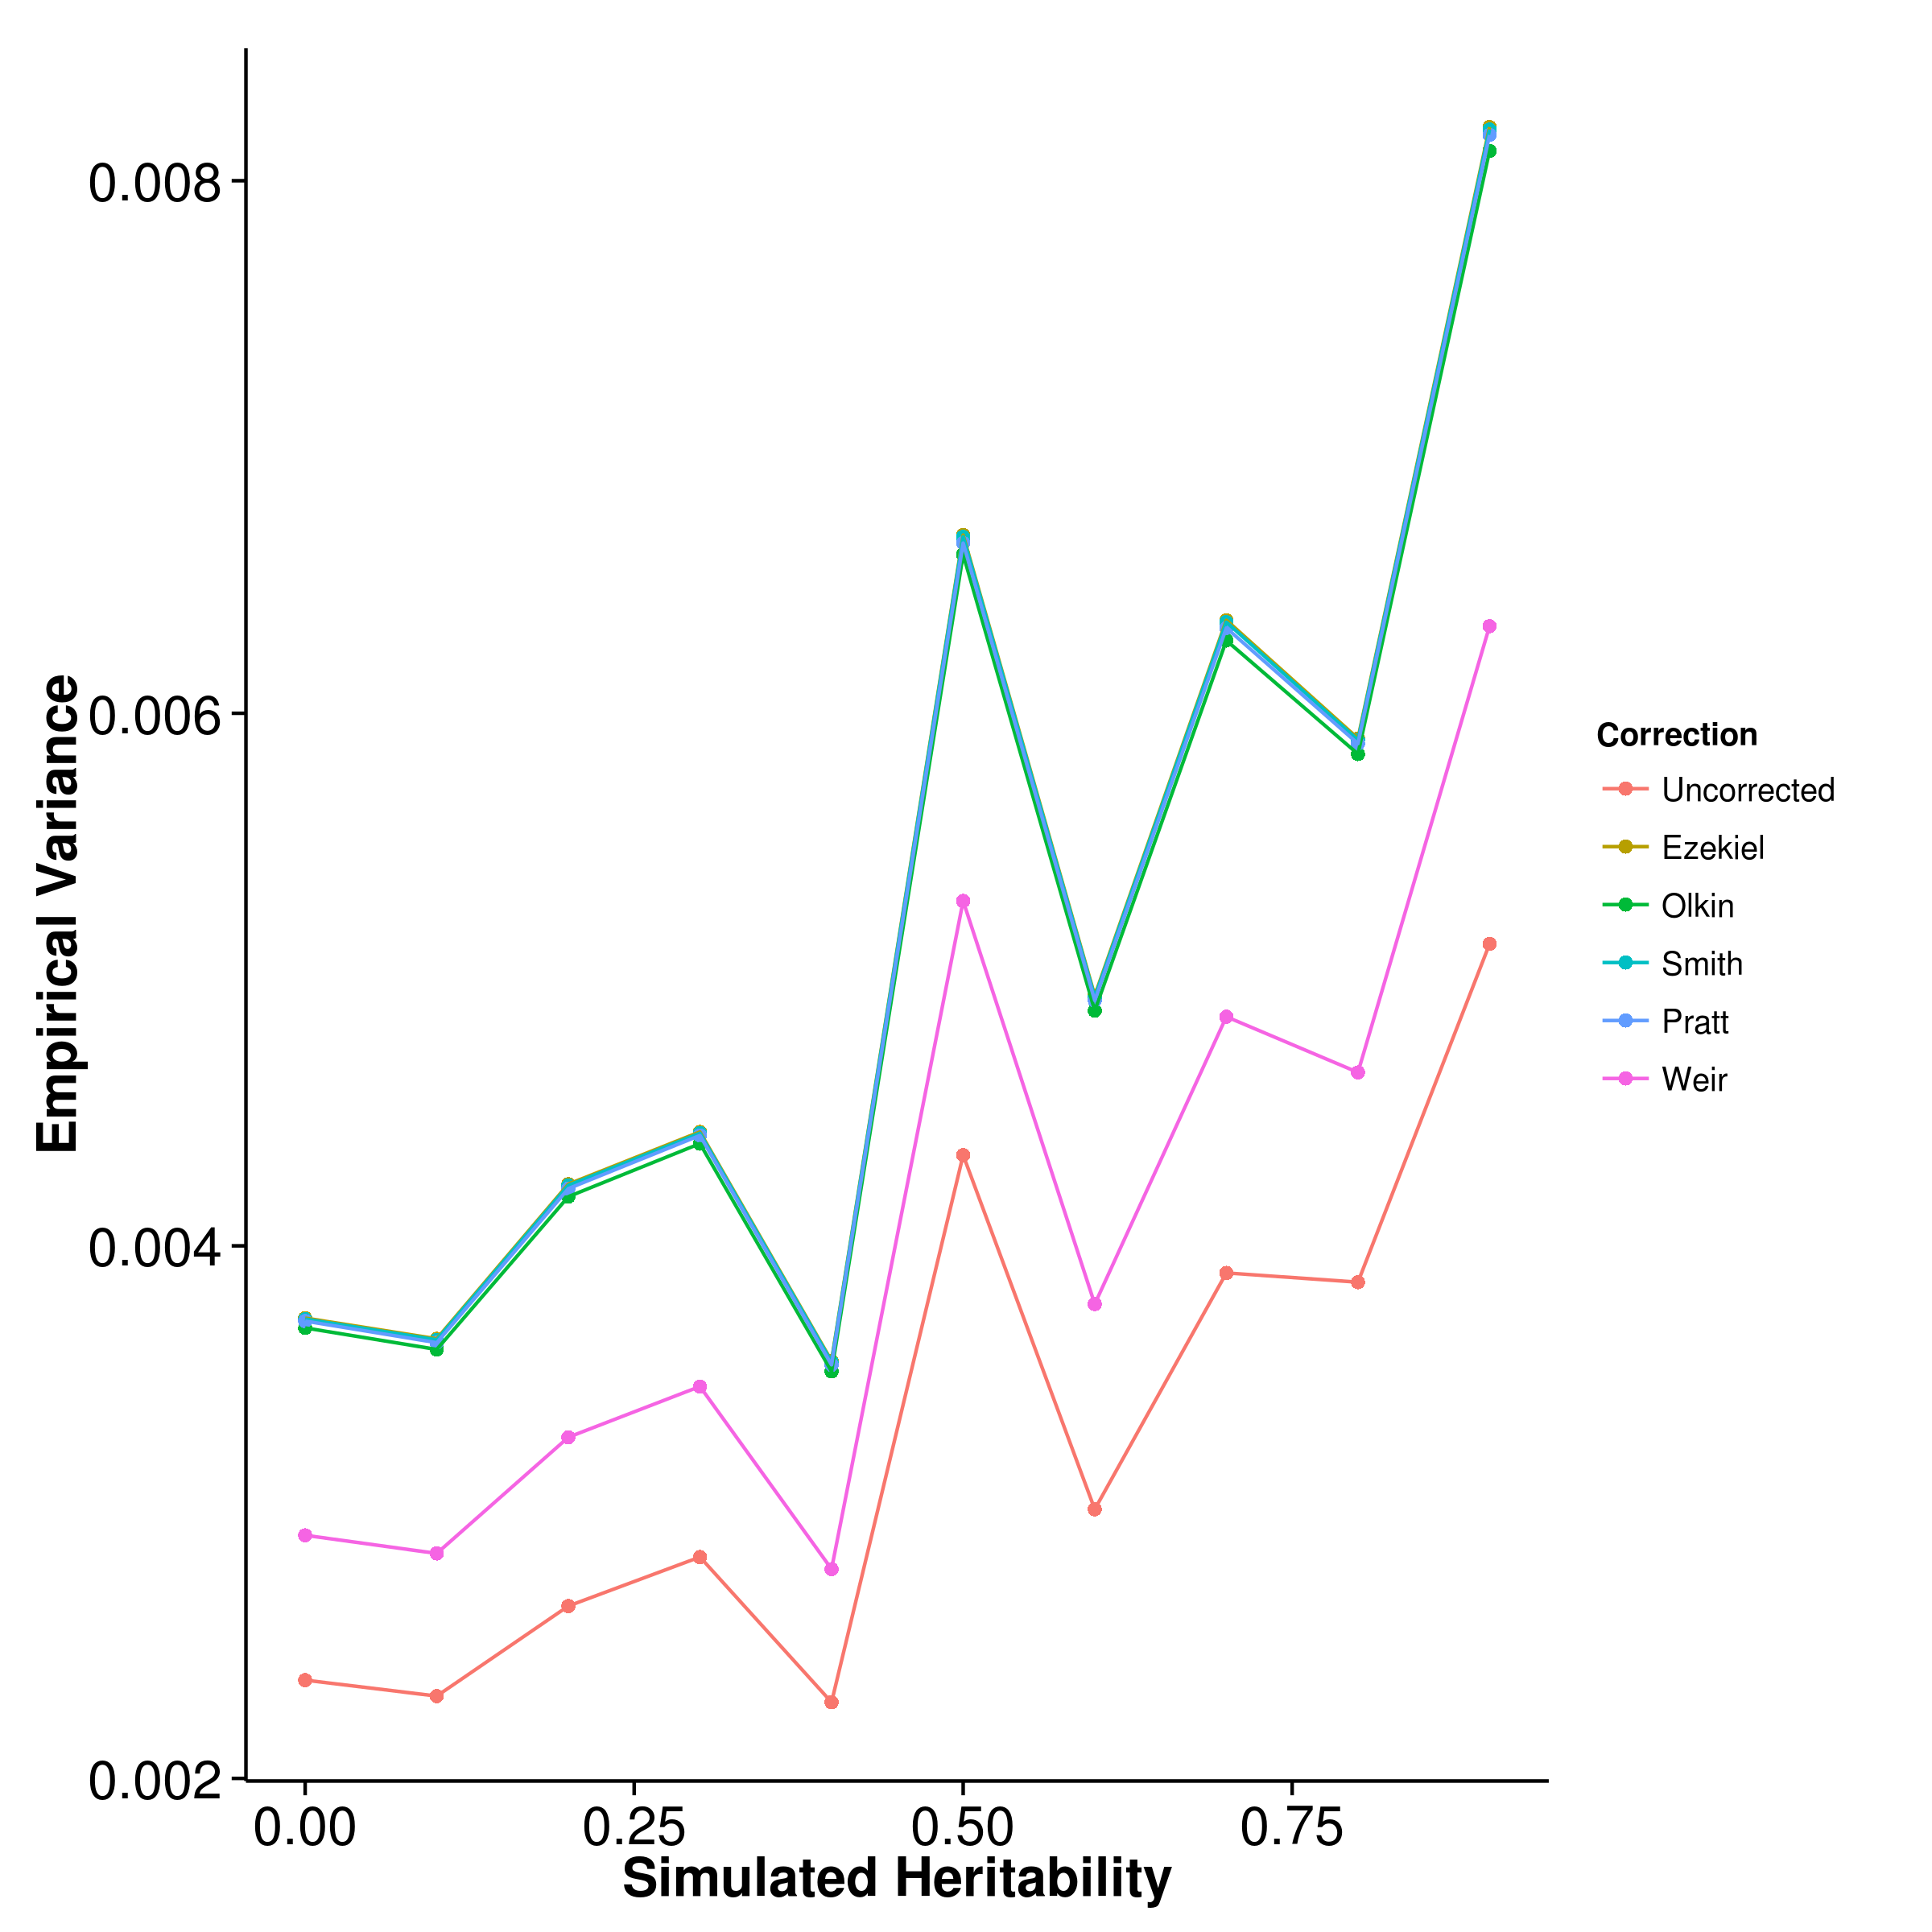
\includegraphics{figure/quantitative/ld_correct/ldCom_var.png}}
				\label{fig:varLDCor}
			}
			\caption[Effect of LD correction to Heritability Estimation]
			{Effect of LD correction to Heritability Estimation.
				We compared the performance of \gls{shrek} when different $R^2$ bias correction algorithm was used.
				When no bias correction was carried out, a downward bias was observed. 
				After the application of the bias correction algorithms, the mean estimations of all except in the case of Weir \cref{eq:weir} algorithms leads to an overestimation of heritability.
			} 
			\label{fig:ldCorCom}
		\end{figure}
		As \gls{shrek} relies on the \gls{LD} structure to estimate the \gls{SNP} heritability, it is important to correct for bias in the \gls{LD} estimates. 
		The performance of the correct algorithms were tested through the HAPGEN2 simulation (\cref{fig:meanLDCor}).
		It is observed that when no bias correction was applied, the mean estimates biased downward, as expected.
		
		On the other hand, all the correction methods, with the exception of the formula proposed by \citet{Weir1980} (\cref{eq:weir}), result in upwardly biased estimates.
		This suggests that most of the bias correction algorithms have ``over-adjusted'' the sampling error, therefore leads to an inflation in the estimates.
		Based on the simulation results, it is concluded that the formula proposed by \citet{Weir1980} works best and are therefore selected as the default \gls{LD} correction algorithm for \gls{shrek}.
		
		\subsection{Comparing with Other Algorithms}
		After the selection of \gls{LD} correction algorithm, it is important to compare the performance of \gls{shrek} with the existing algorithms.
		Another aim of the current study is to investigate how different sampling strategies and genetic architectures influence the performance of \gls{ldsc}.
		Therefore a series of extensive simulation analyses were performed. 
		
		\subsubsection{Quantitative Trait Simulation}
			%Mean
			\begin{figure}
				\centering
				\subfloat[SHREK]{
					\scalebox{.4}{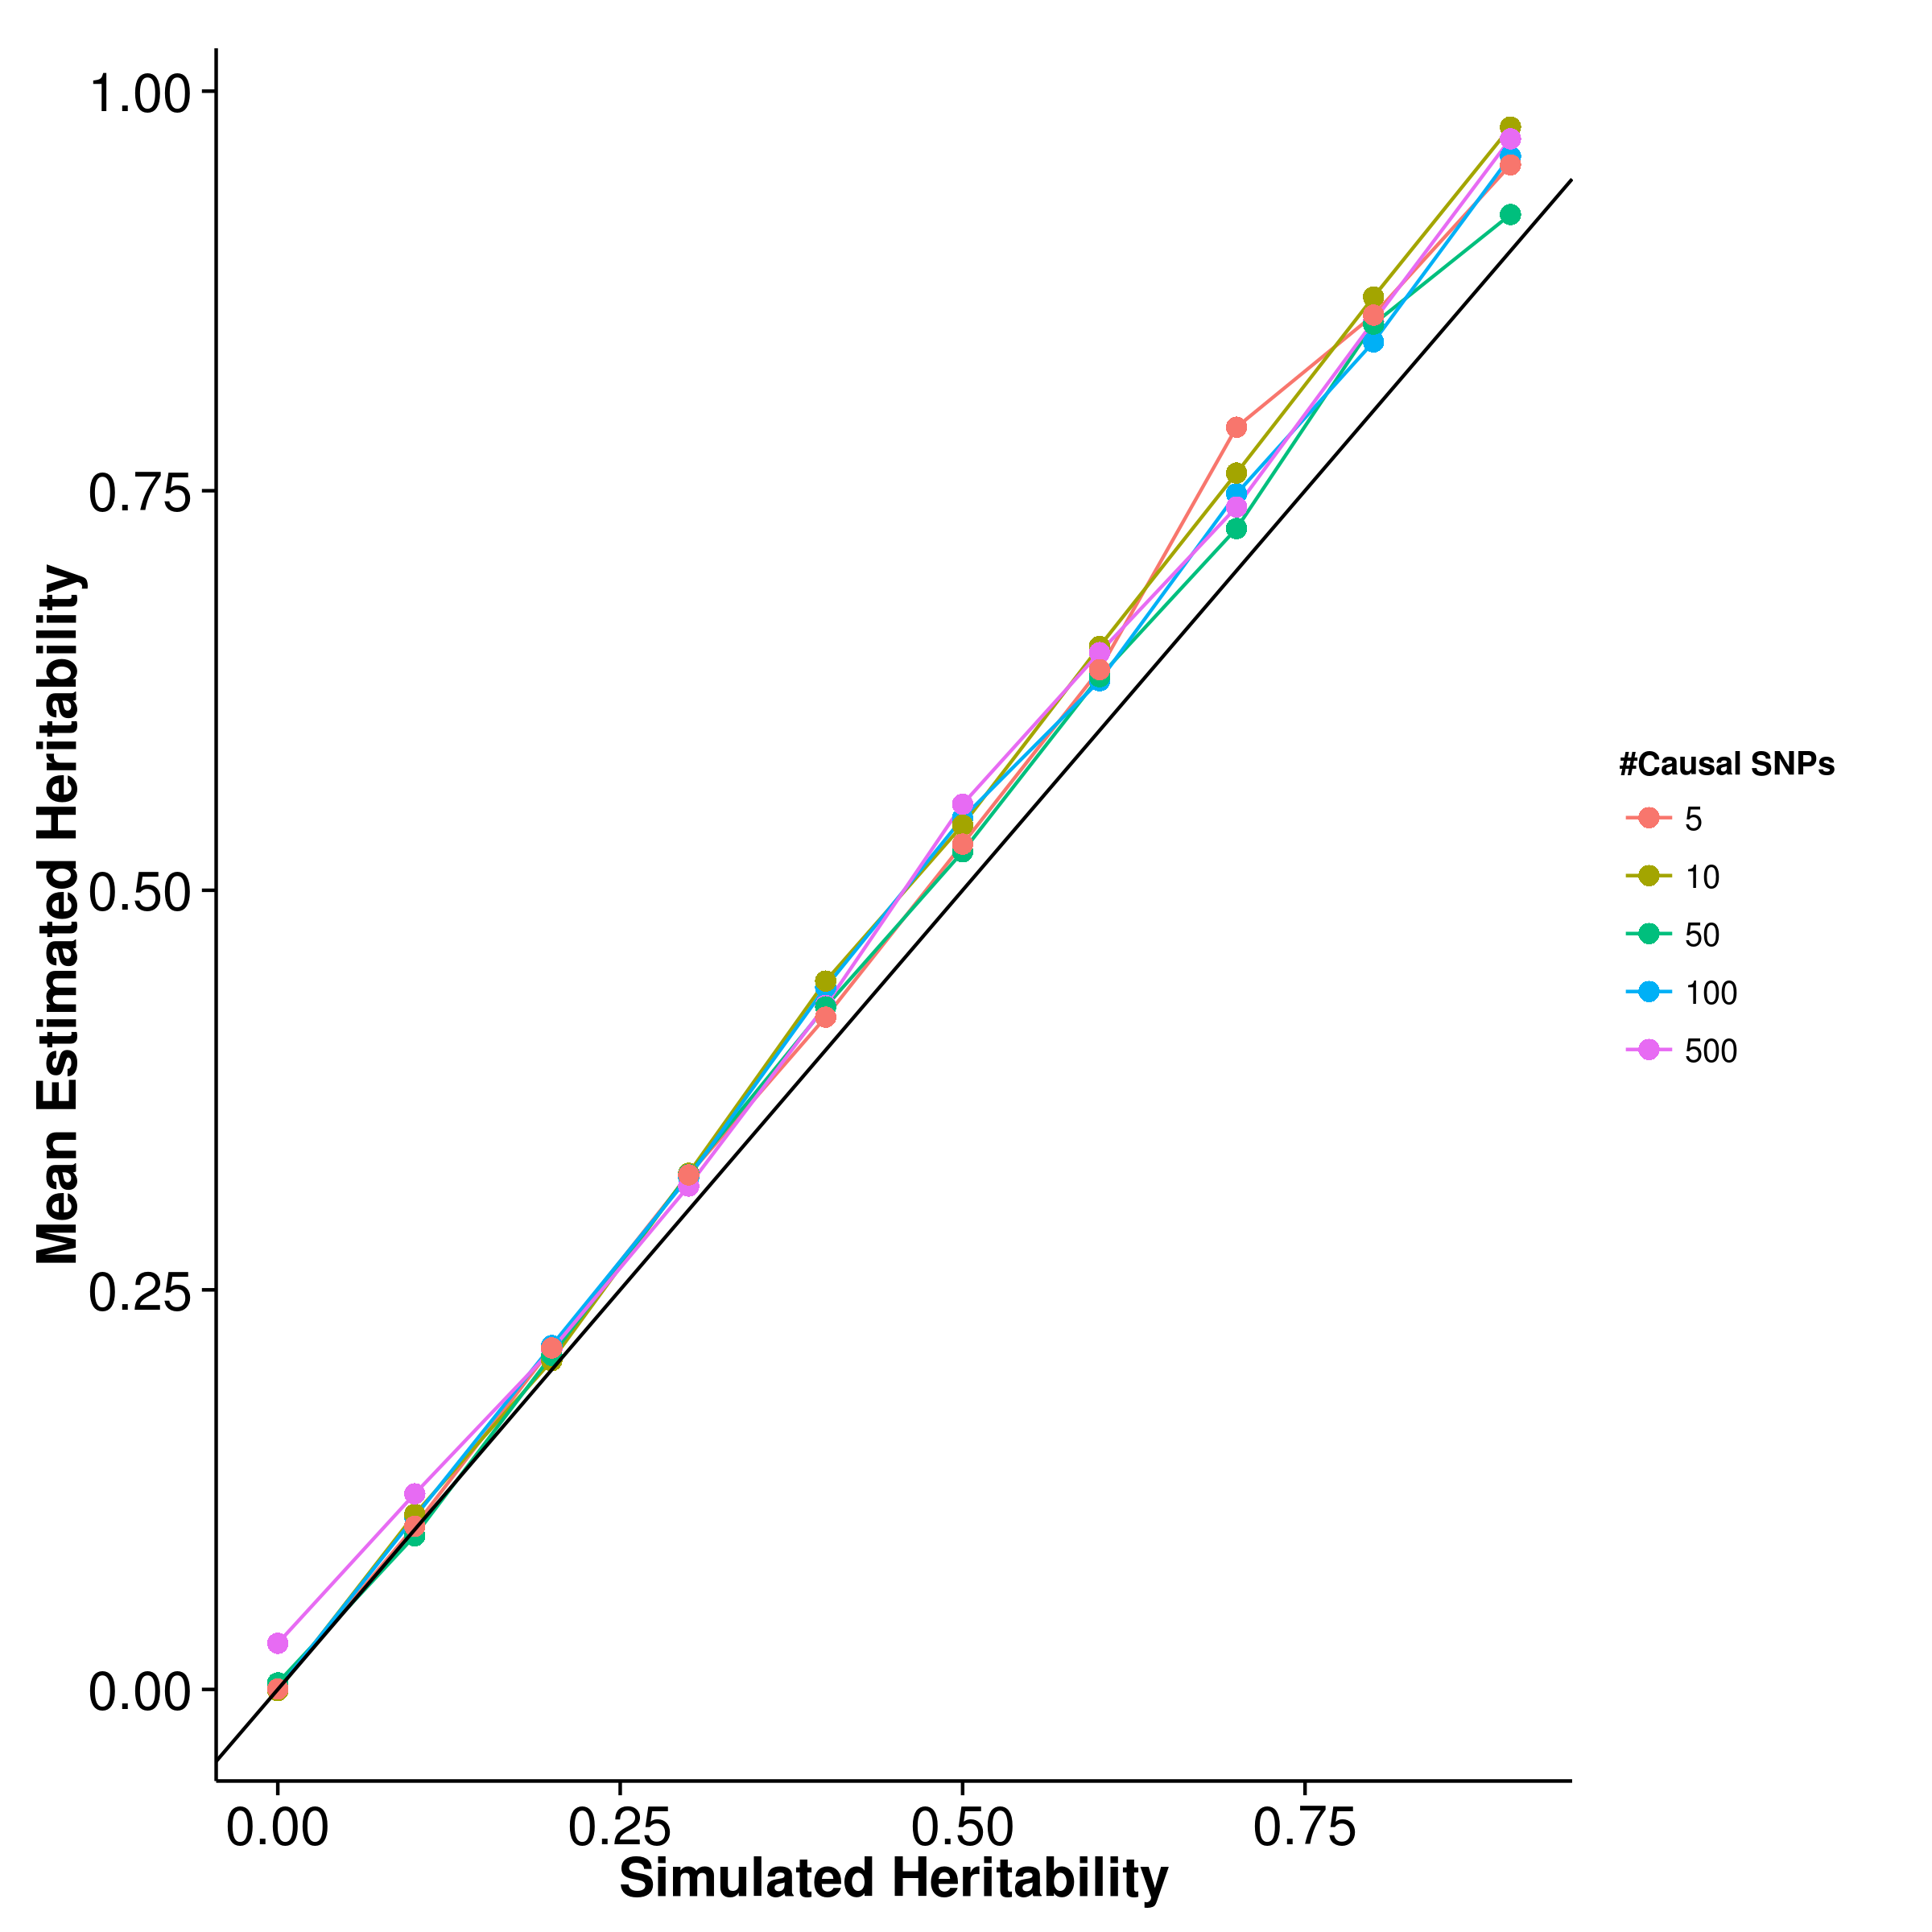
\includegraphics{figure/he_summary/random/shrek_Qt_Rand_mean.png}}
					\label{fig:shrekQtRandMean}
				}
				\subfloat[GCTA]{
					\scalebox{.4}{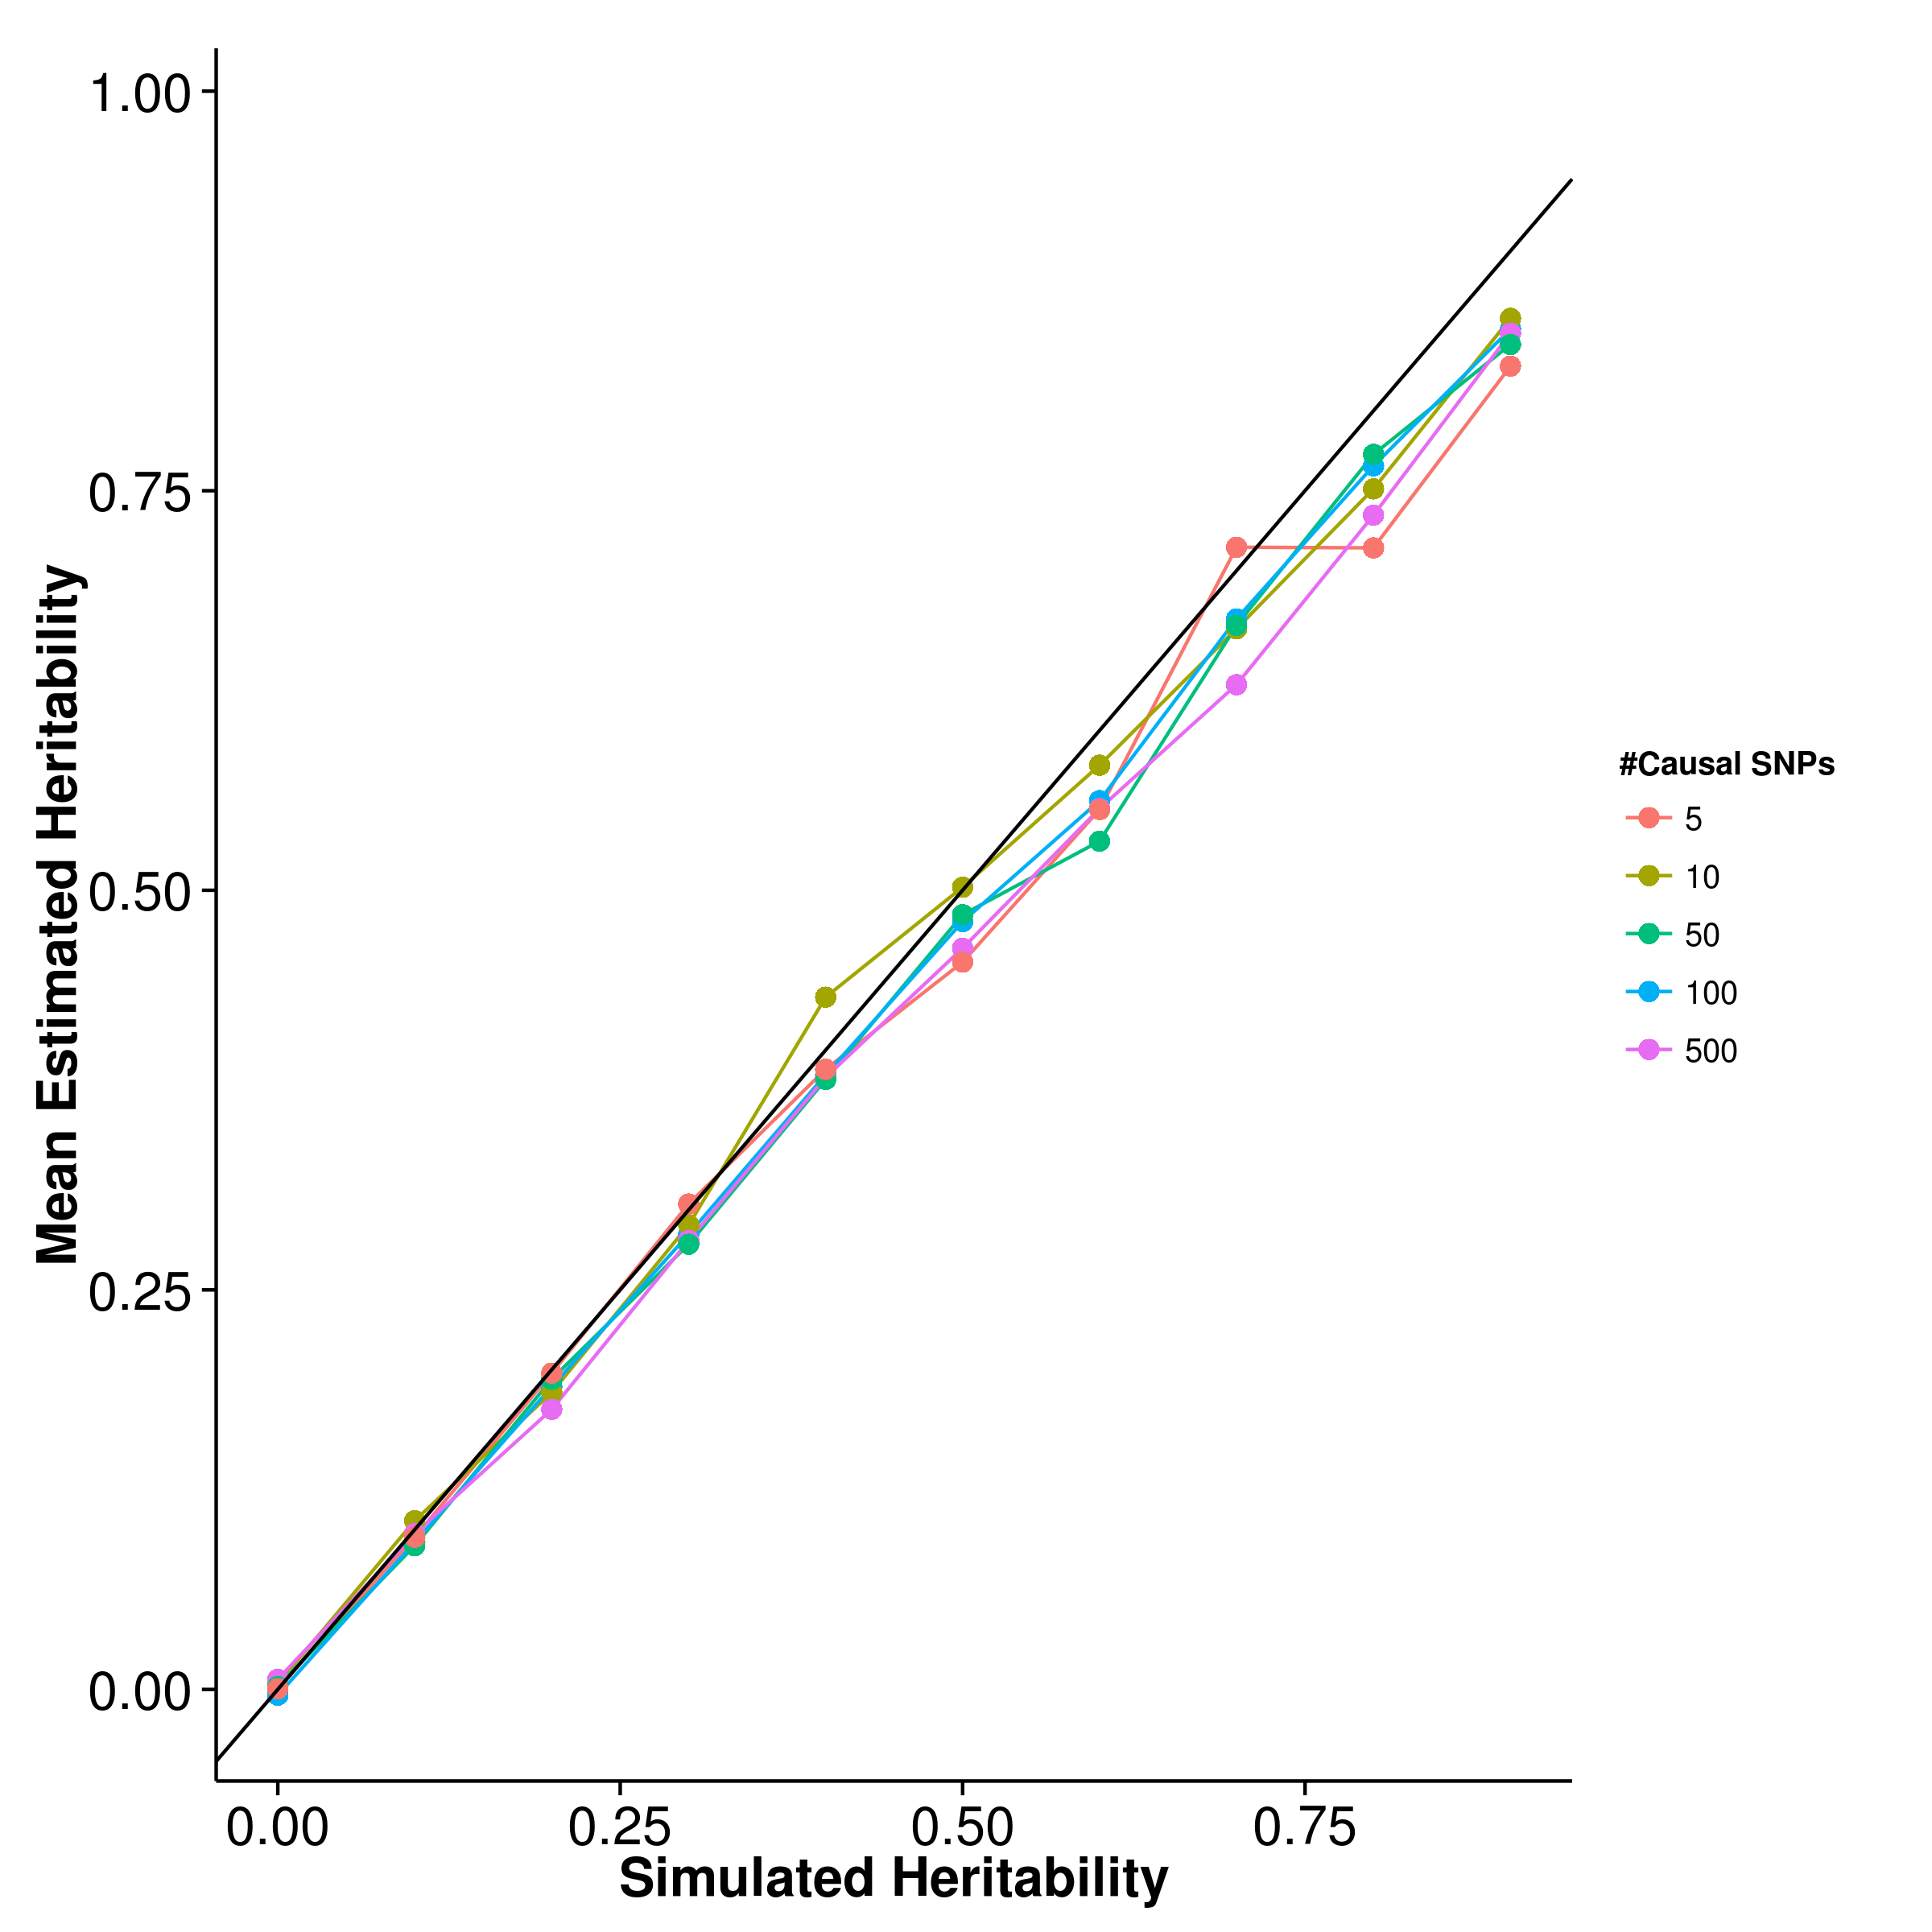
\includegraphics{figure/he_summary/random/gcta_Qt_Rand_mean.png}}
					\label{fig:gctaQtRandMean}
				}\\
				\subfloat[LDSC with fix intercept]{
					\scalebox{.4}{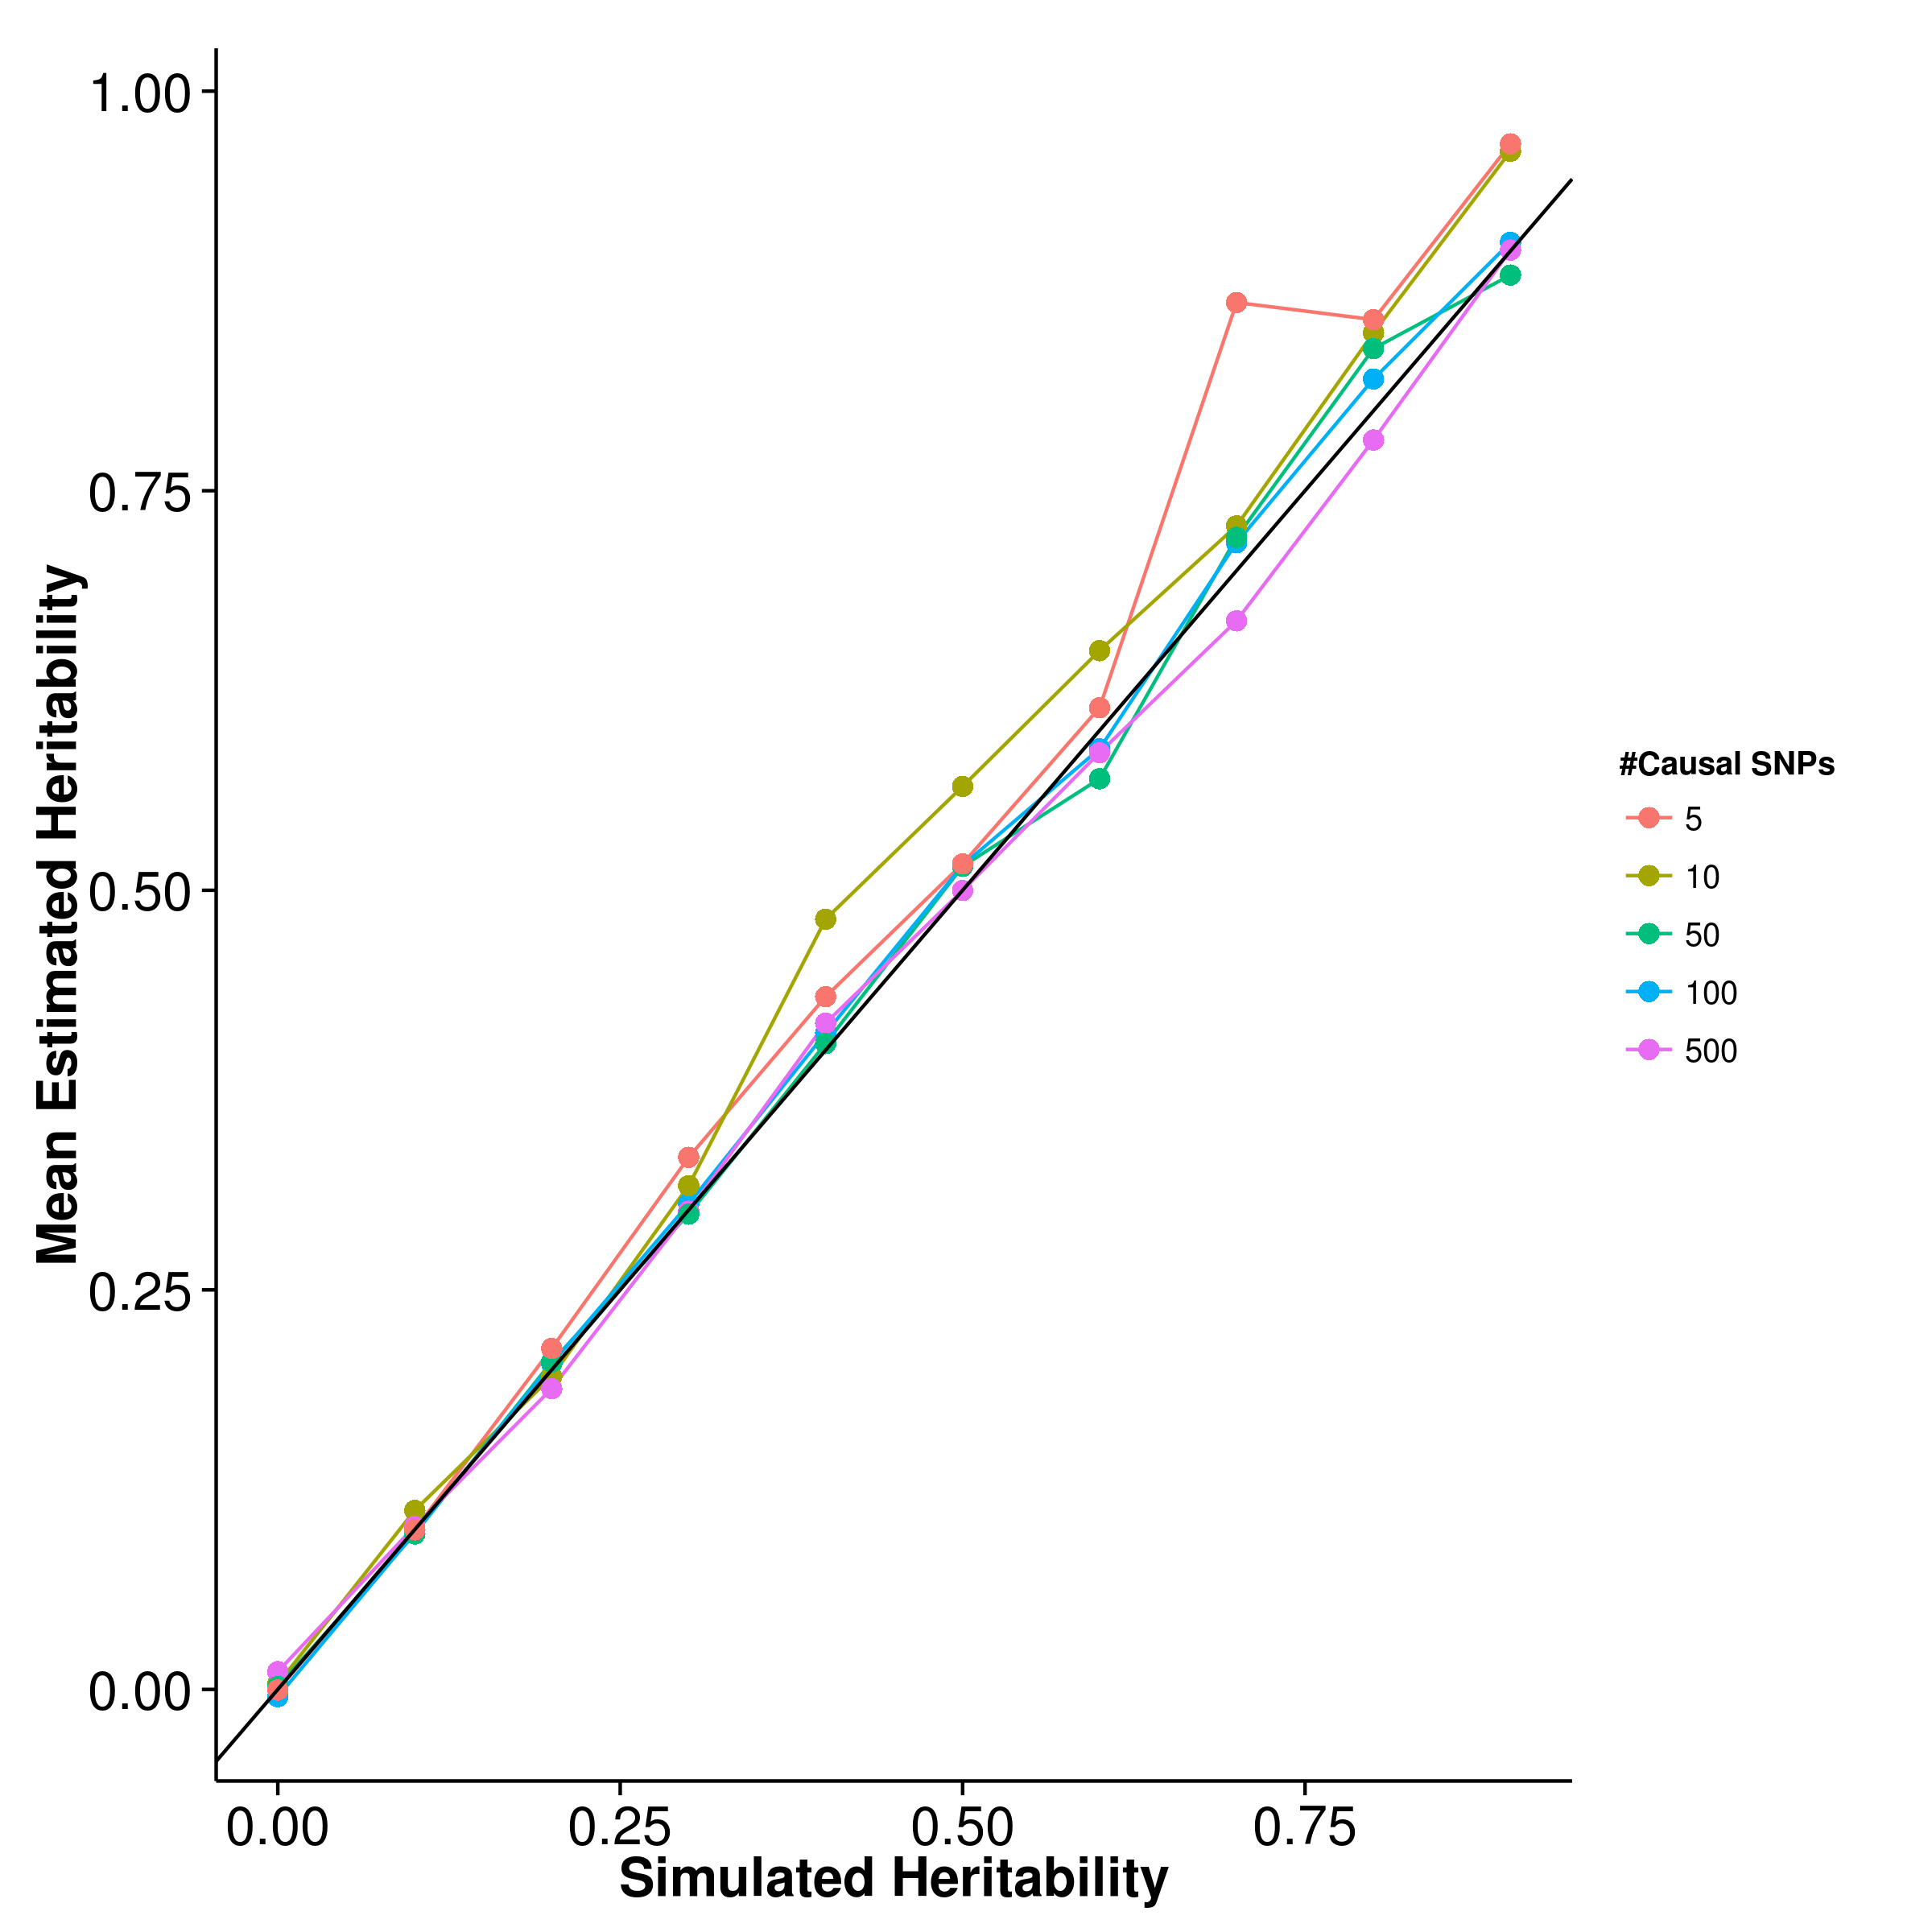
\includegraphics{figure/he_summary/random/ldsc_Qt_Rand_mean.png}}
					\label{fig:ldscQtRandMean}
				}
				\subfloat[LDSC with intercept estimation]{
					
					\scalebox{.4}{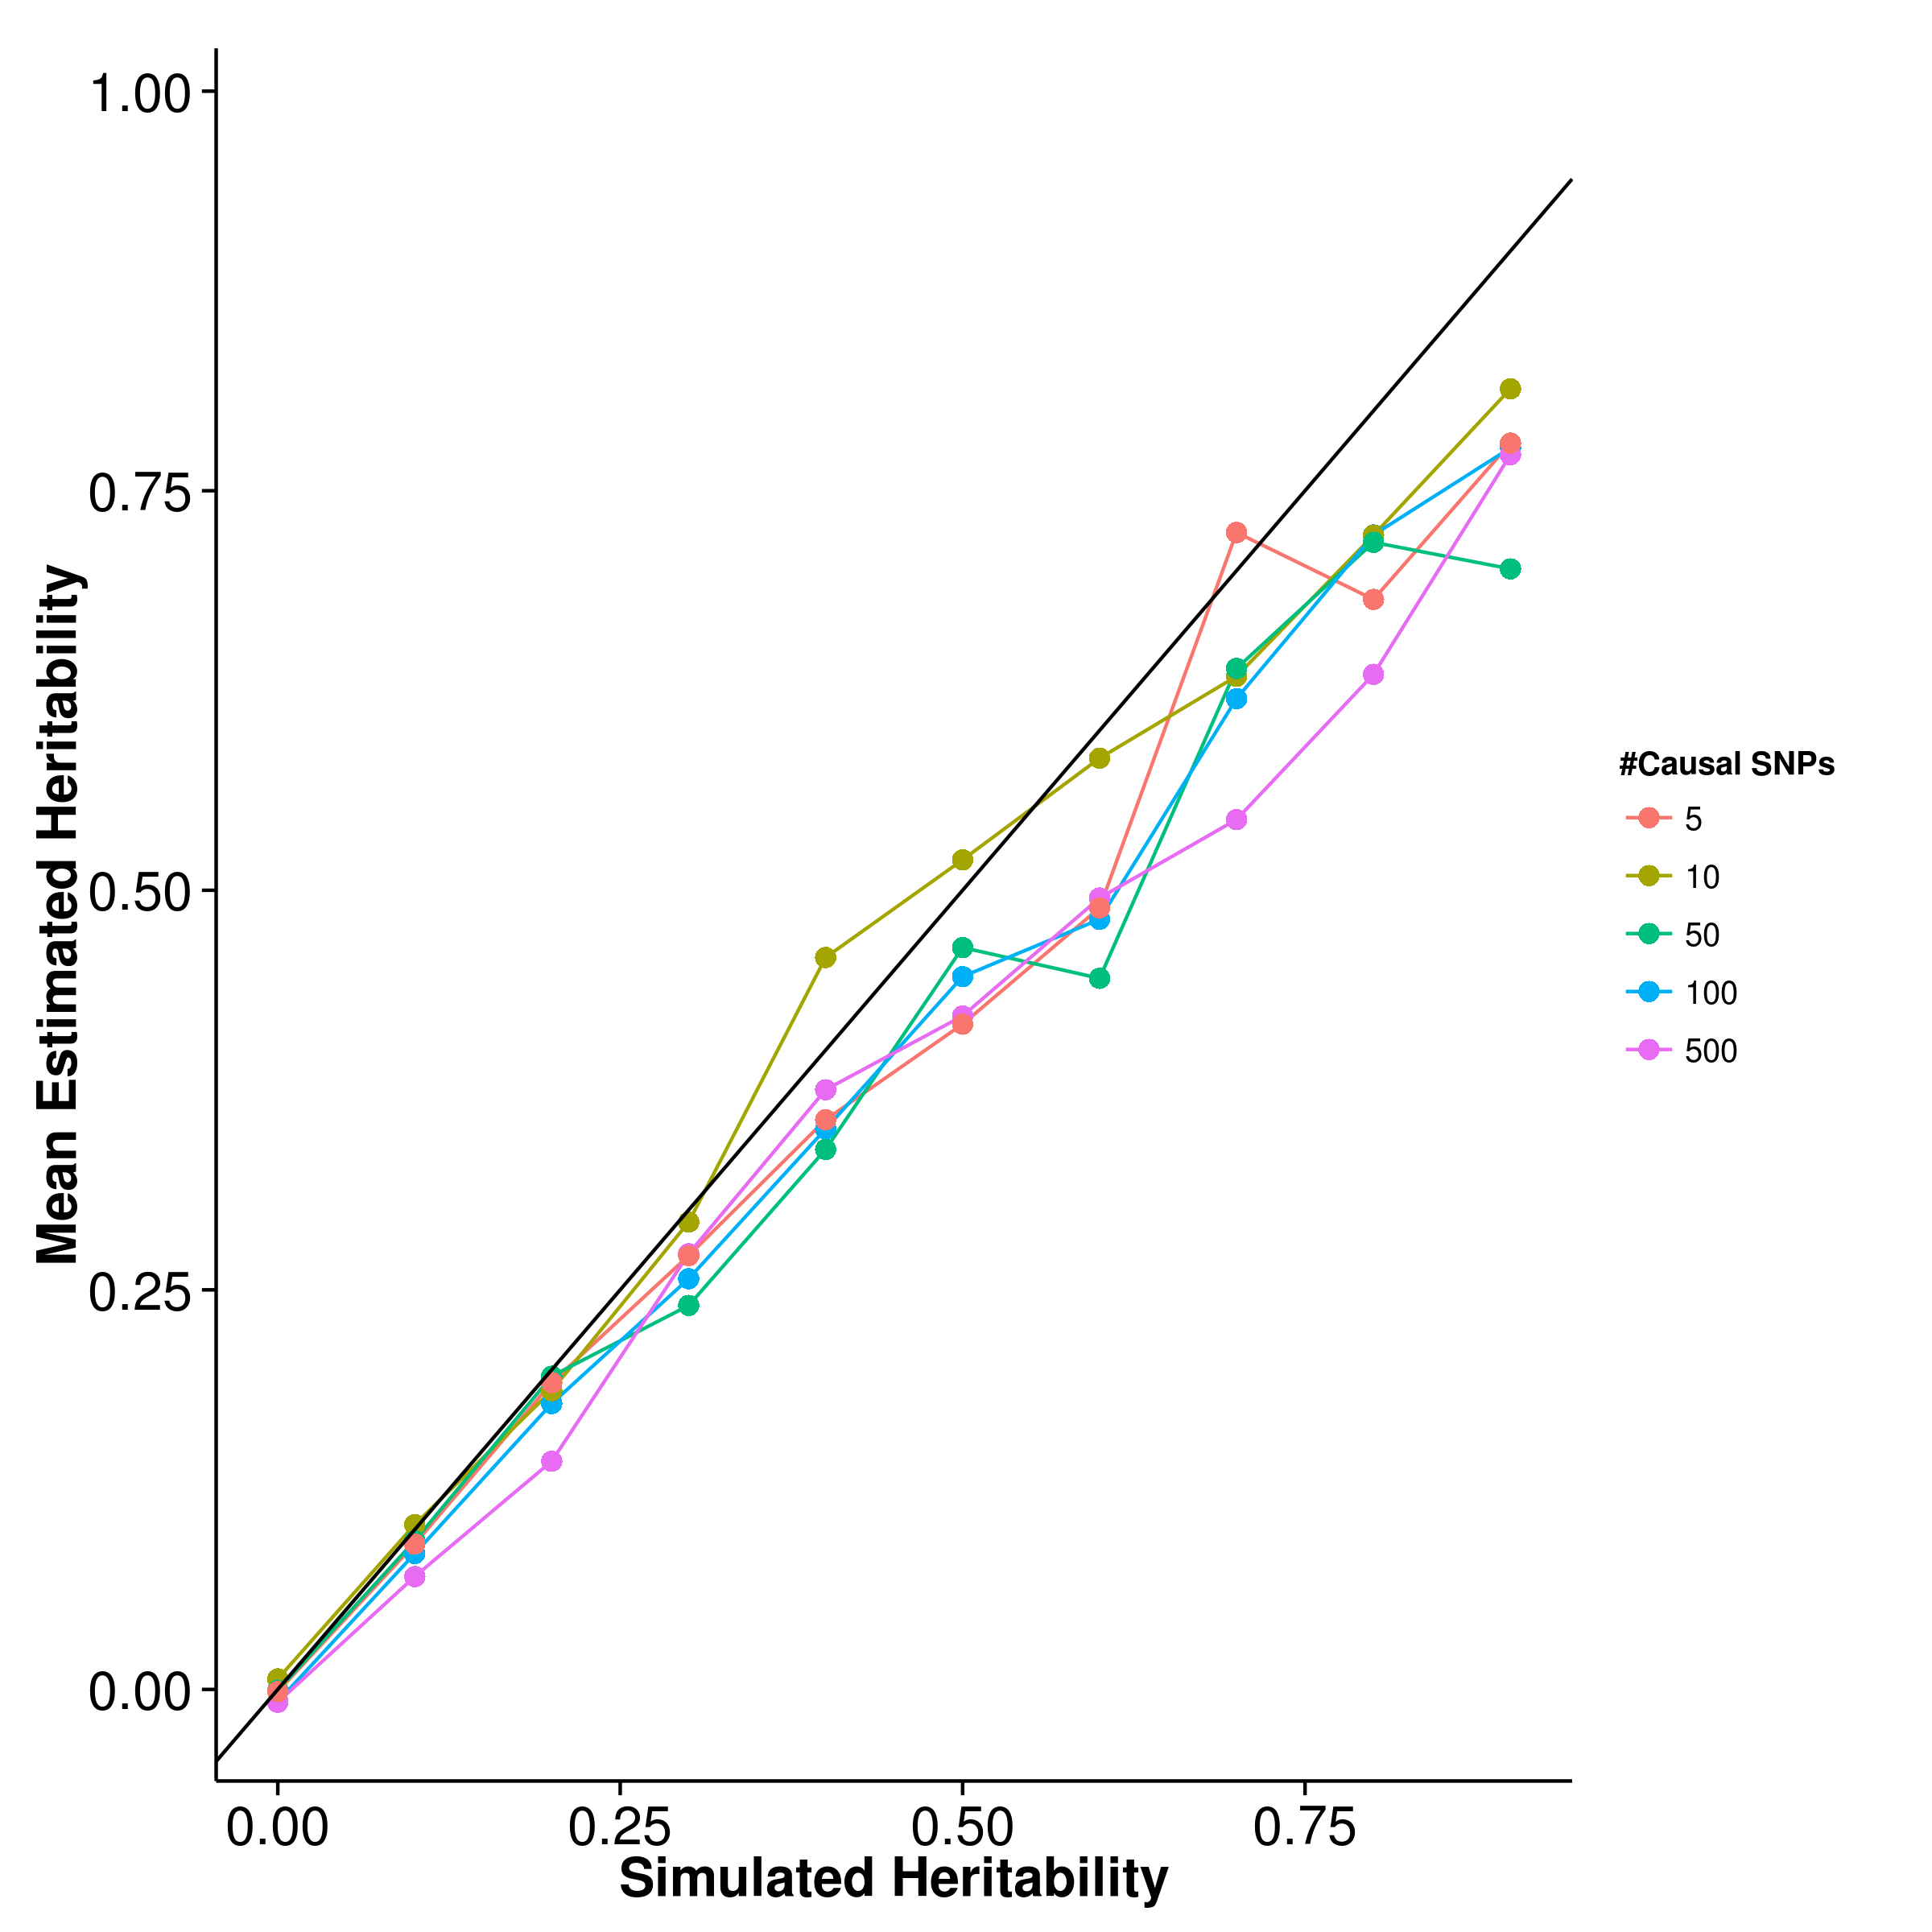
\includegraphics{figure/he_summary/random/ldscIn_Qt_Rand_mean.png}}
					\label{fig:ldscInQtRandMean}
				}
				\caption[Mean of Quantitative Trait Simulation Results]
				{Mean of results from quantitative trait simulation with random effect size simulation.
					Estimations form \gls{shrek} were slightly biased upwards whereas \gls{gcta} and \gls{ldsc} with intercept estimations both biased downwards.
					On the other hand, \gls{ldsc} with fixed intercept provides least biased estimates under polygenic conditions. 
					However, when the number of causal \glspl{SNP} is small (e.g. 5 or 10), an upward bias was observed.} 
				\label{fig:QtRandMean}
			\end{figure}
			%Variance
			\begin{figure}
				\centering
				\subfloat[SHREK]{
					\scalebox{.4}{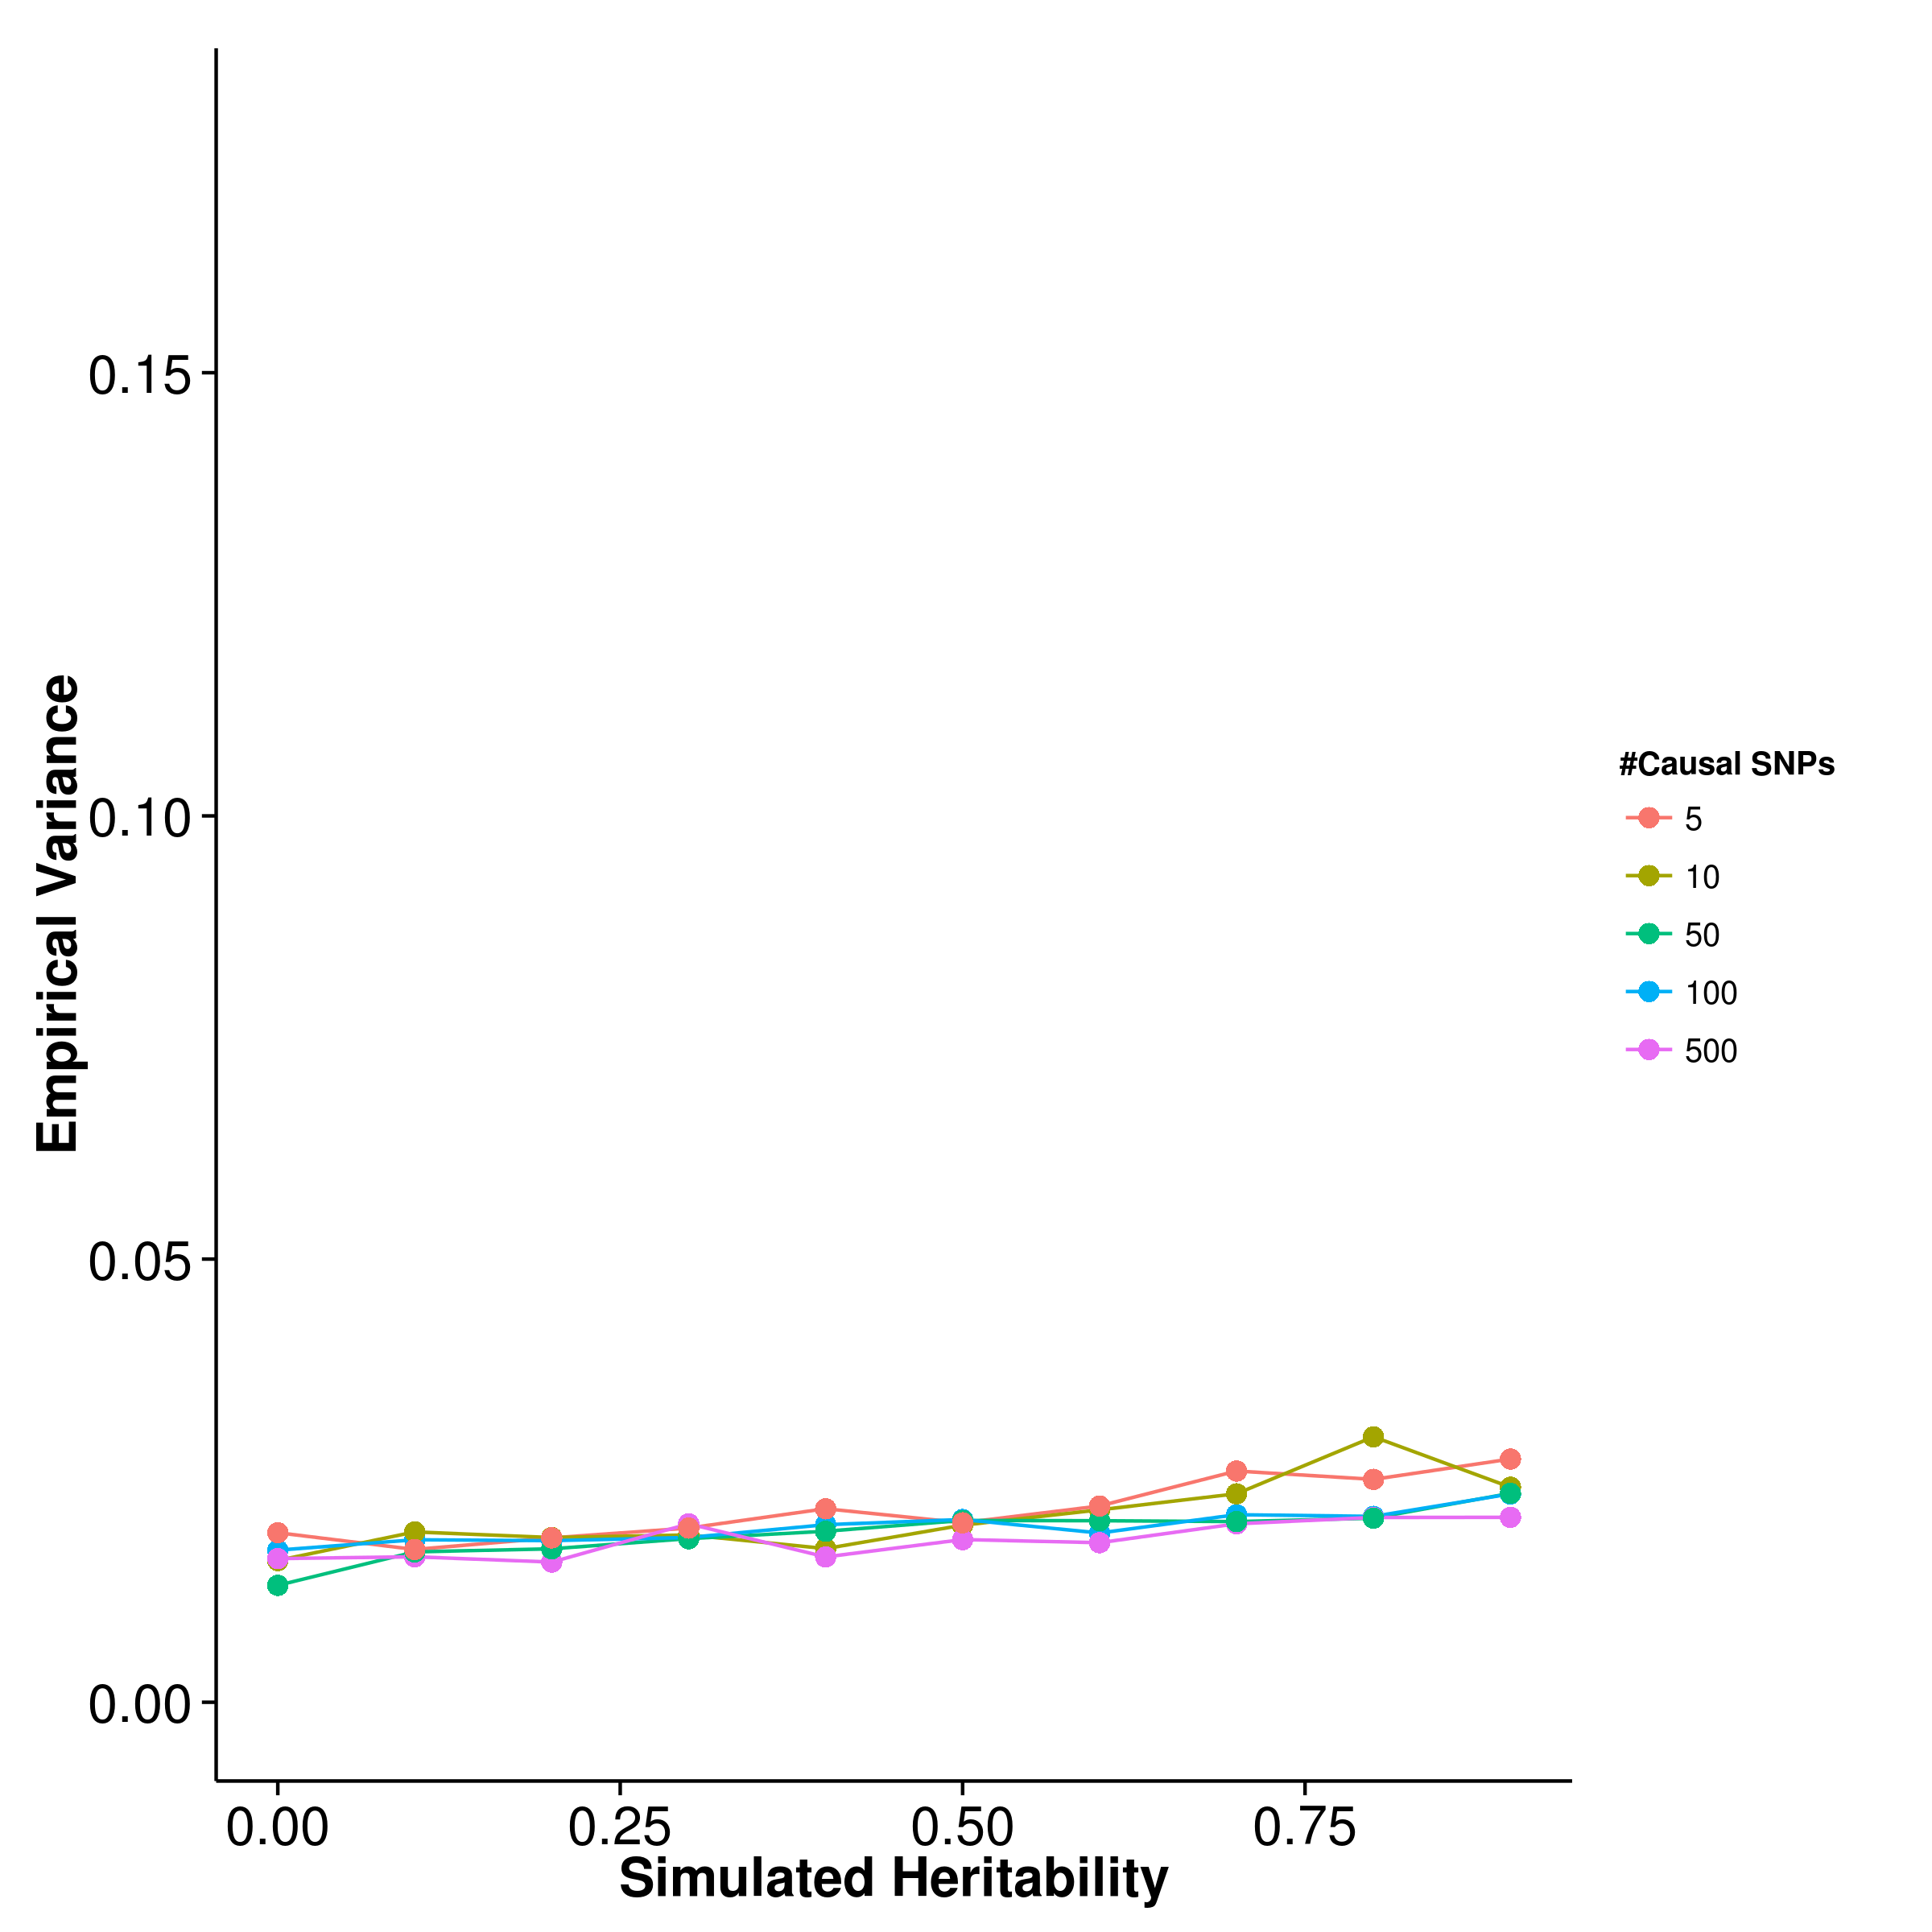
\includegraphics{figure/he_summary/random/shrek_Qt_Rand_sd.png}}
					\label{fig:shrekQtRandVar}
				}
				\subfloat[GCTA]{
					\scalebox{.4}{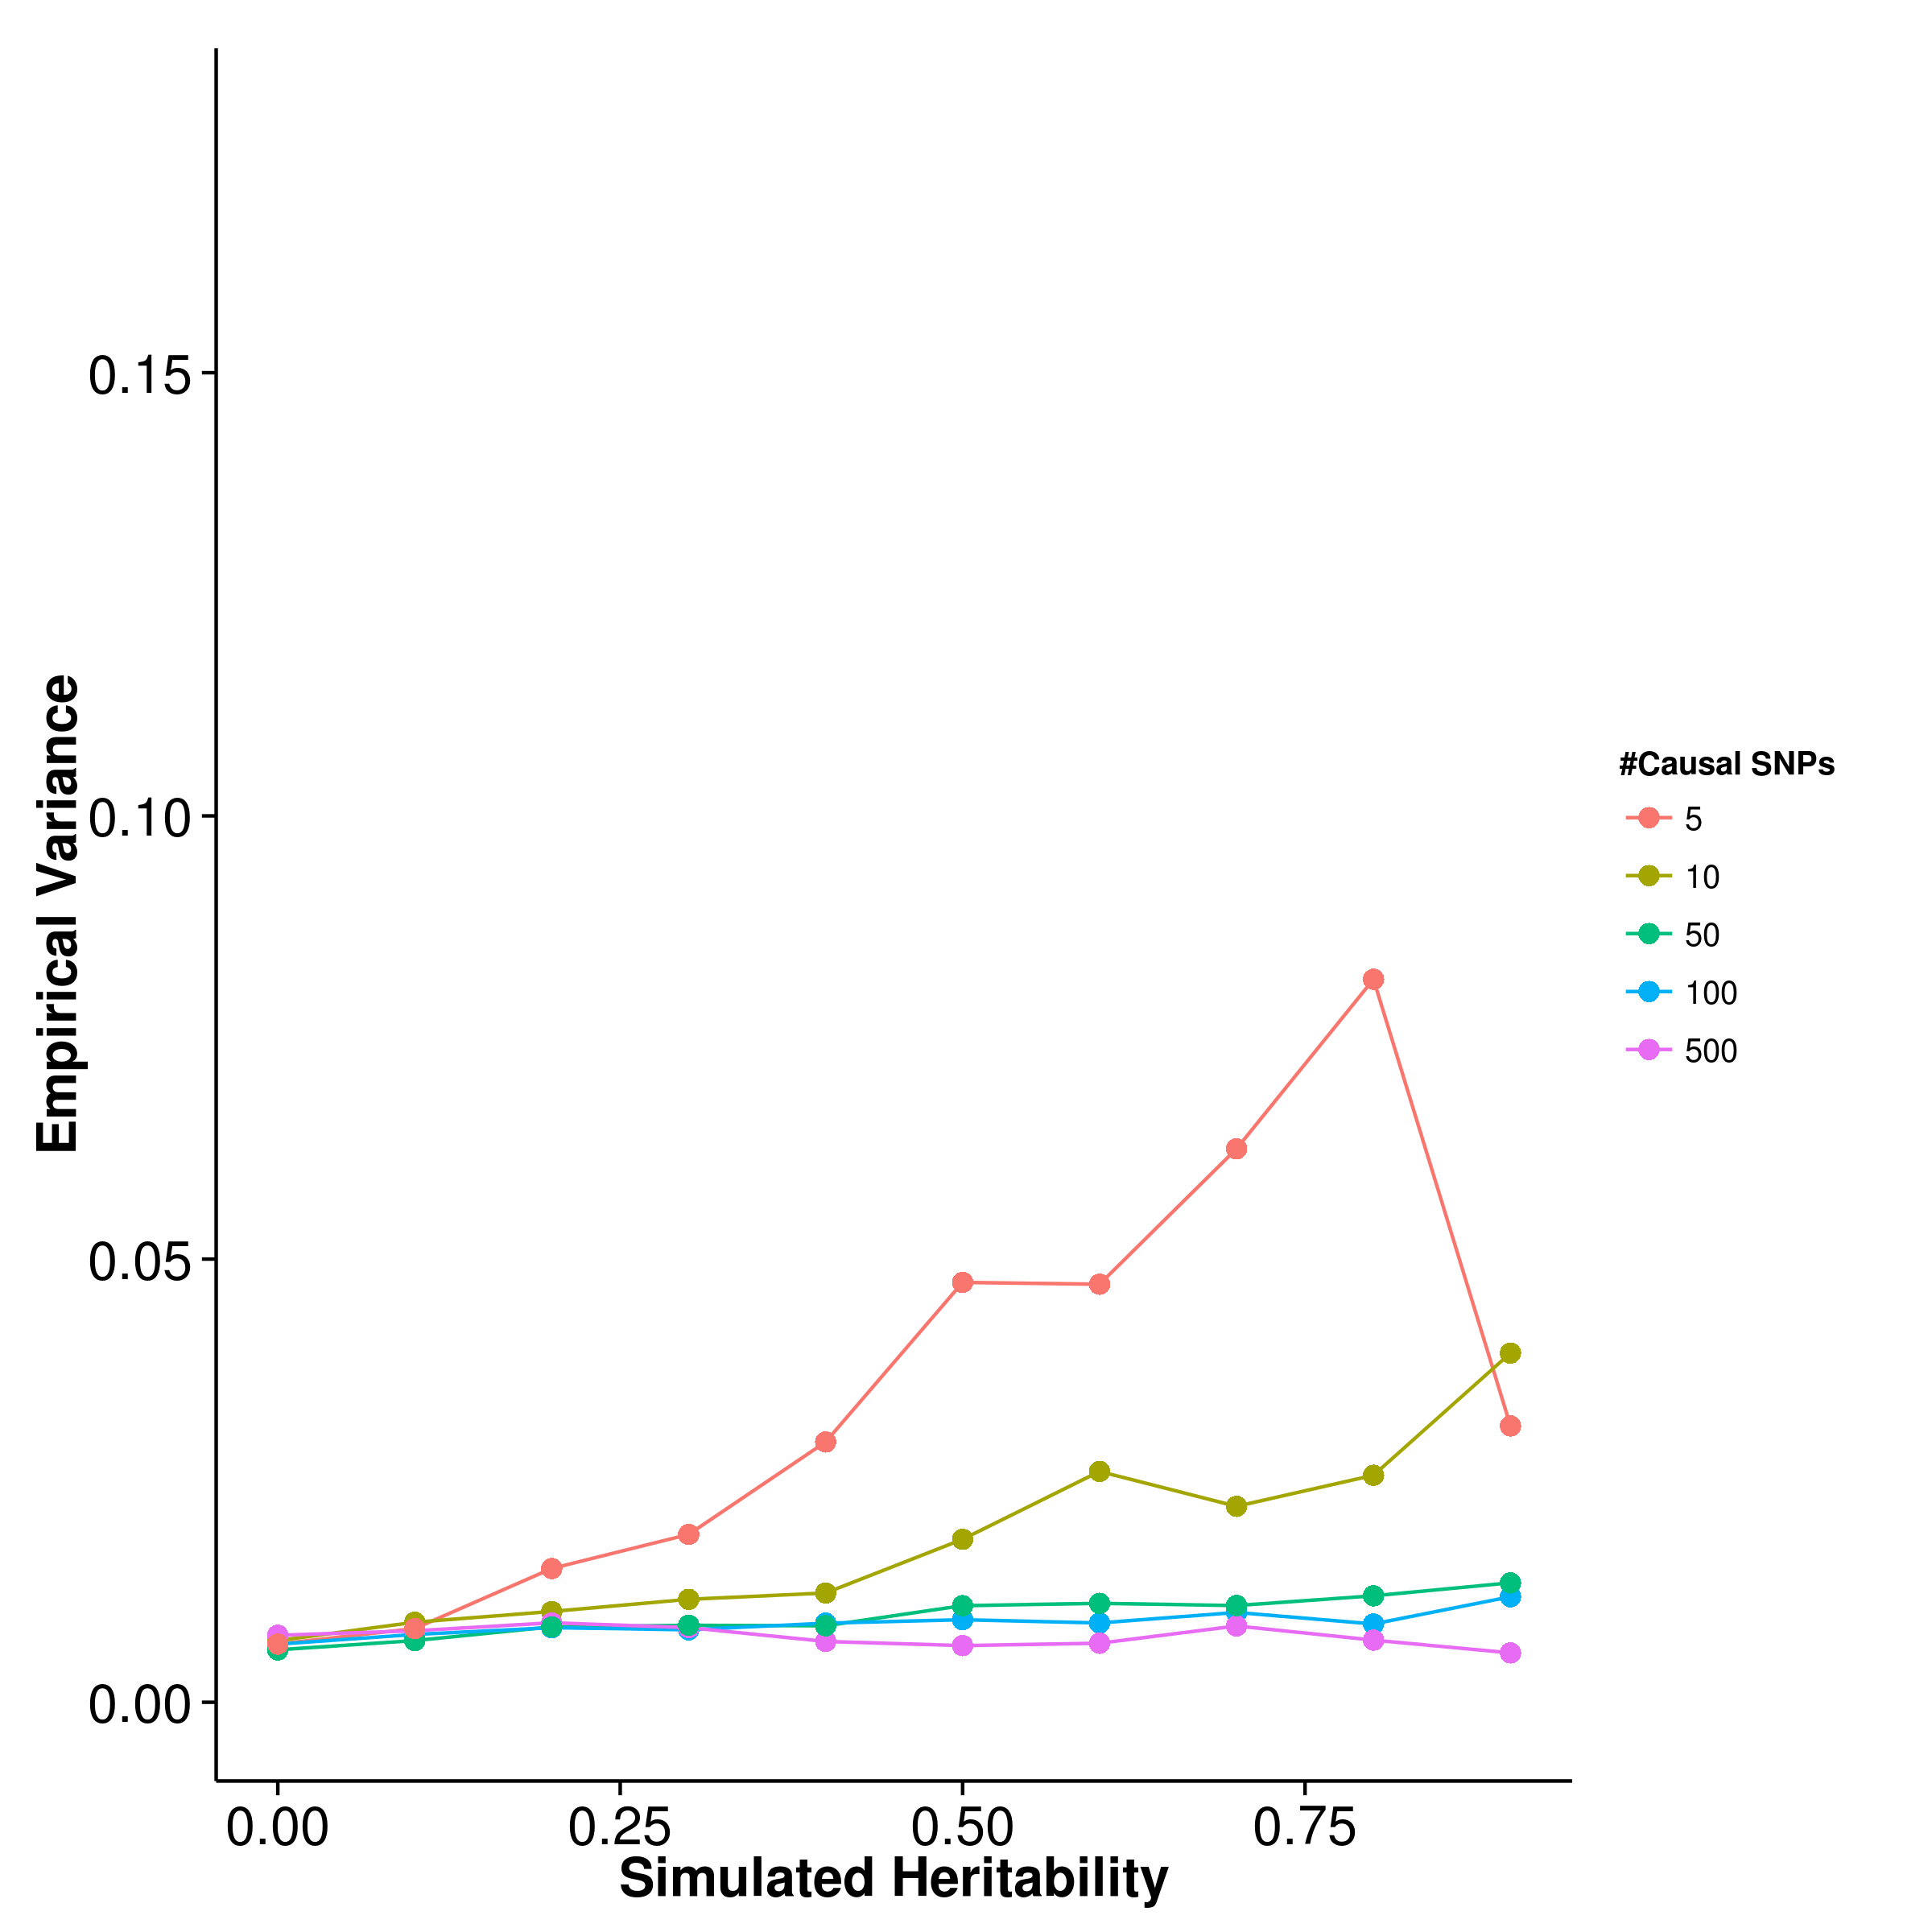
\includegraphics{figure/he_summary/random/gcta_Qt_Rand_sd.png}}
					\label{fig:gctaQtRandVar}
				}\\
				\subfloat[LDSC with fix intercept]{
					\scalebox{.4}{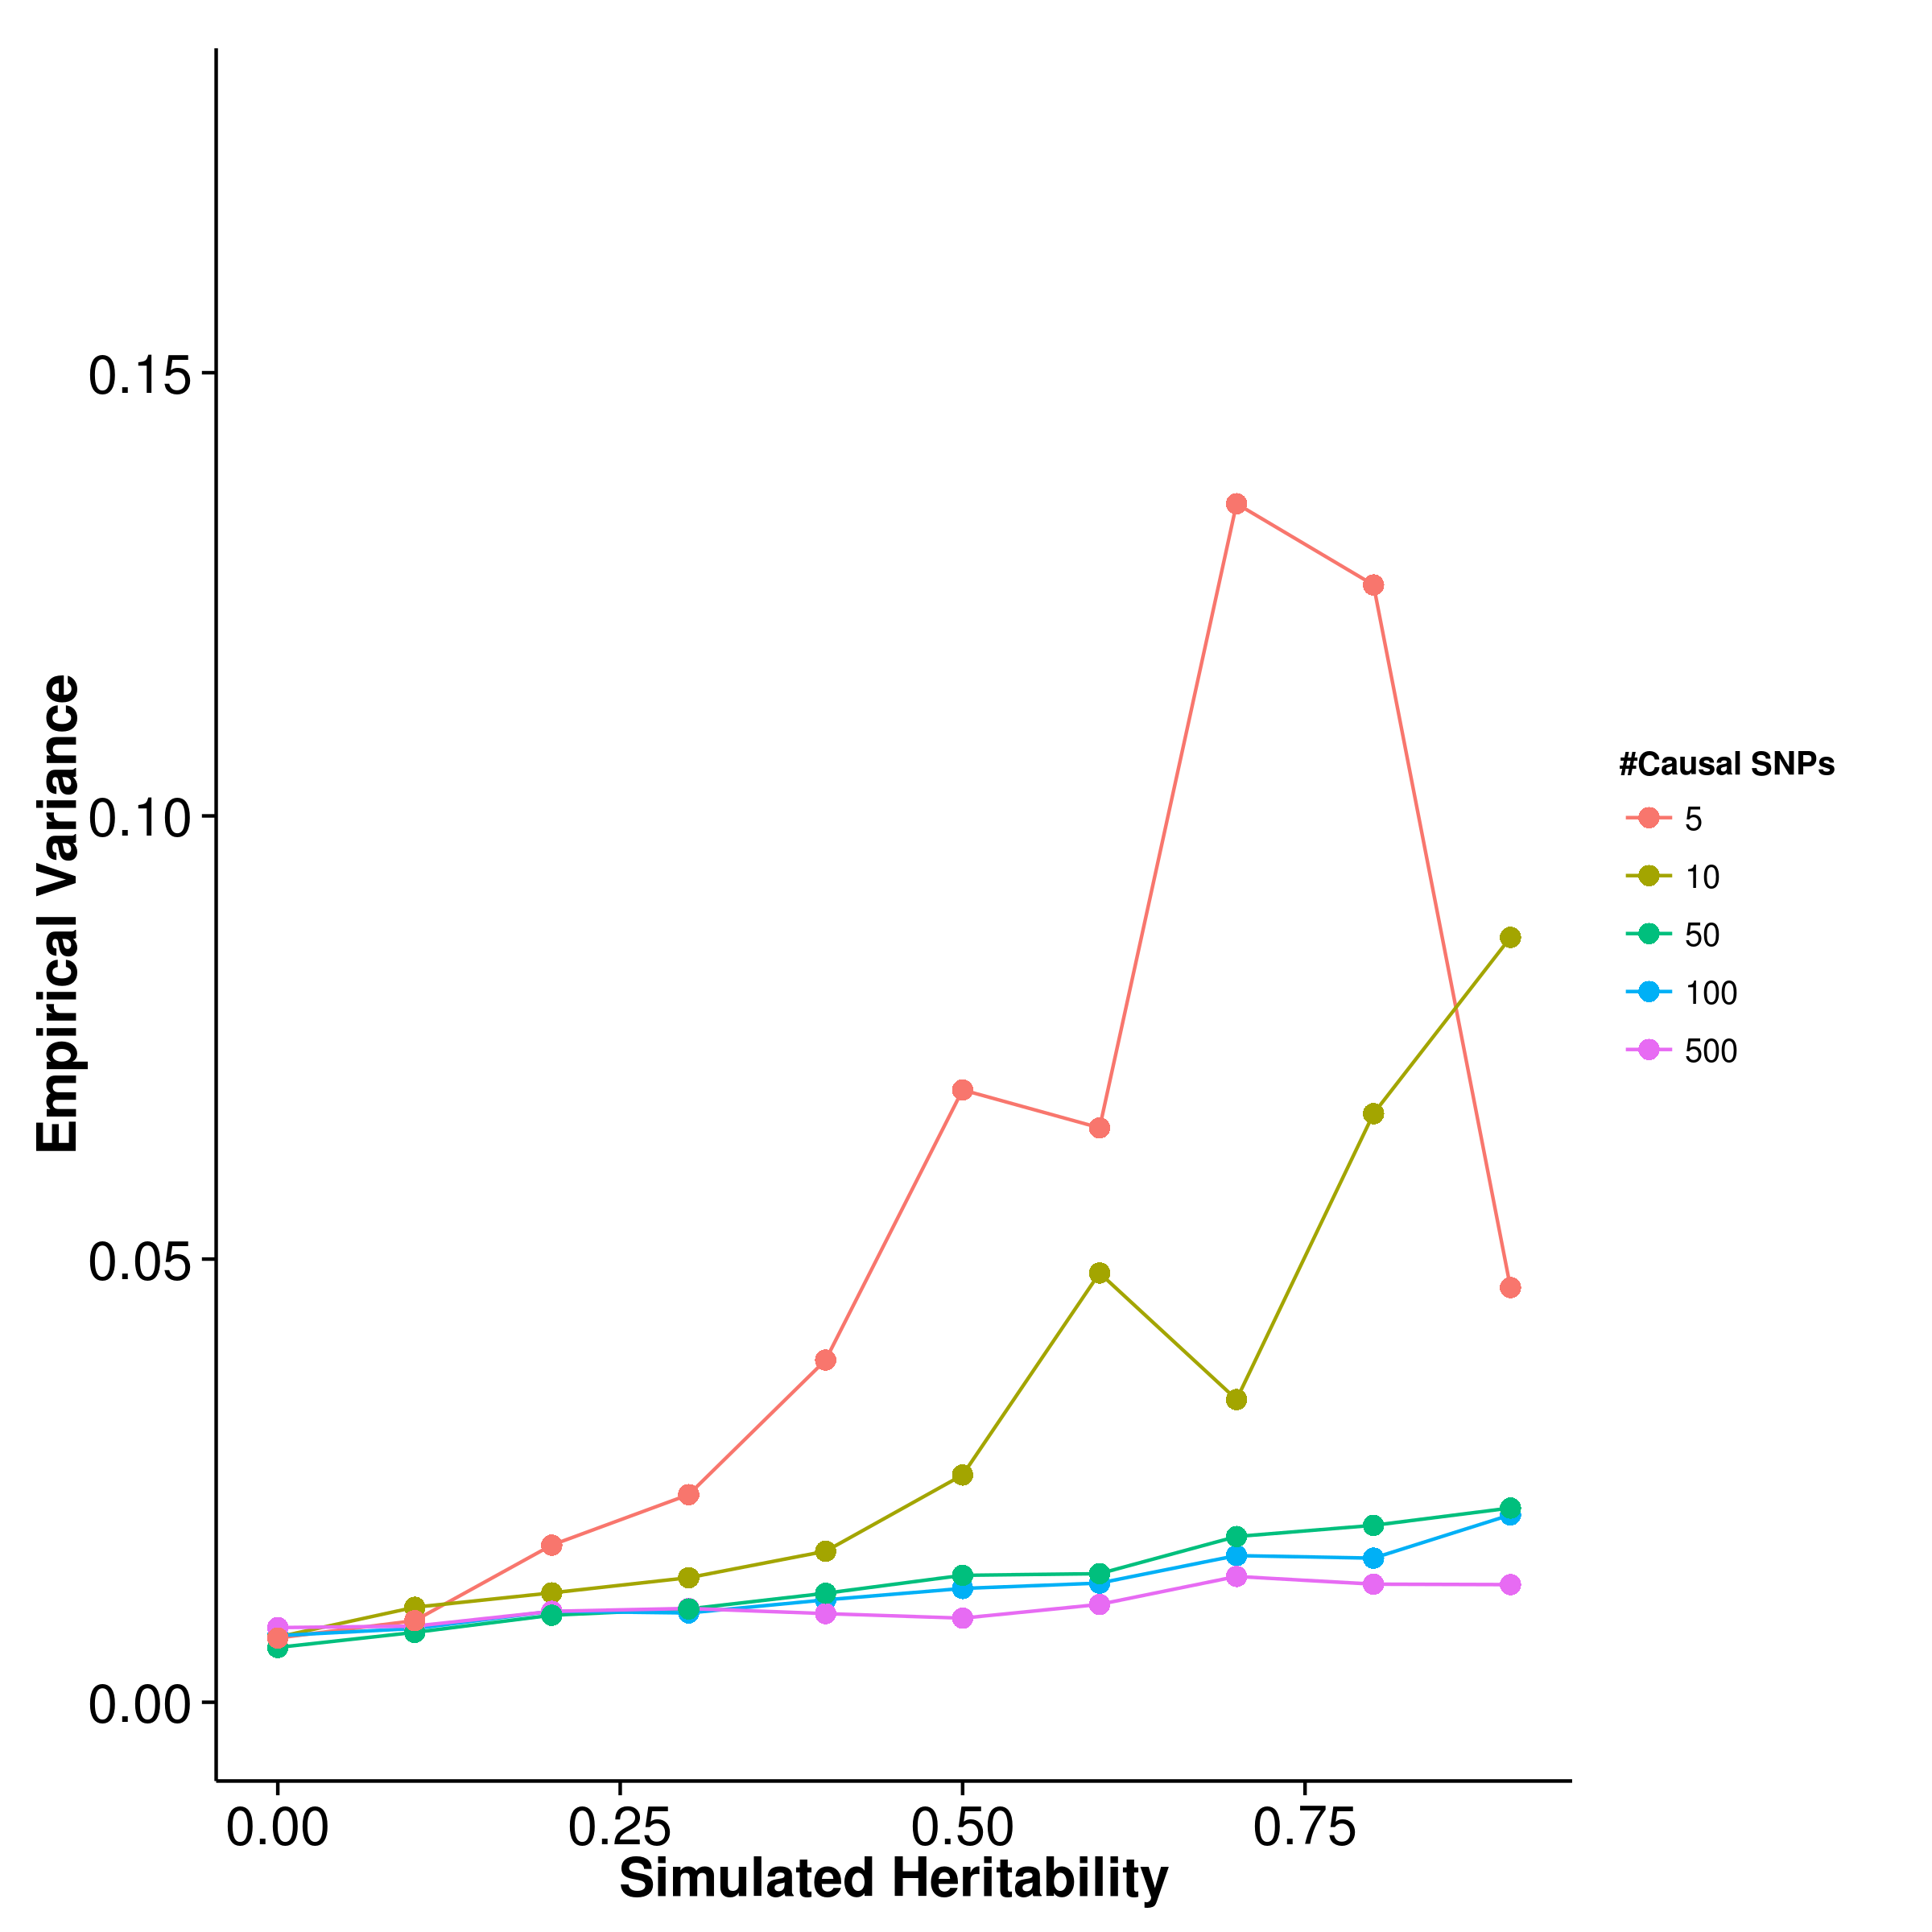
\includegraphics{figure/he_summary/random/ldsc_Qt_Rand_sd.png}}
					\label{fig:ldscQtRandVar}
				}
				\subfloat[LDSC with intercept estimation]{
					
					\scalebox{.4}{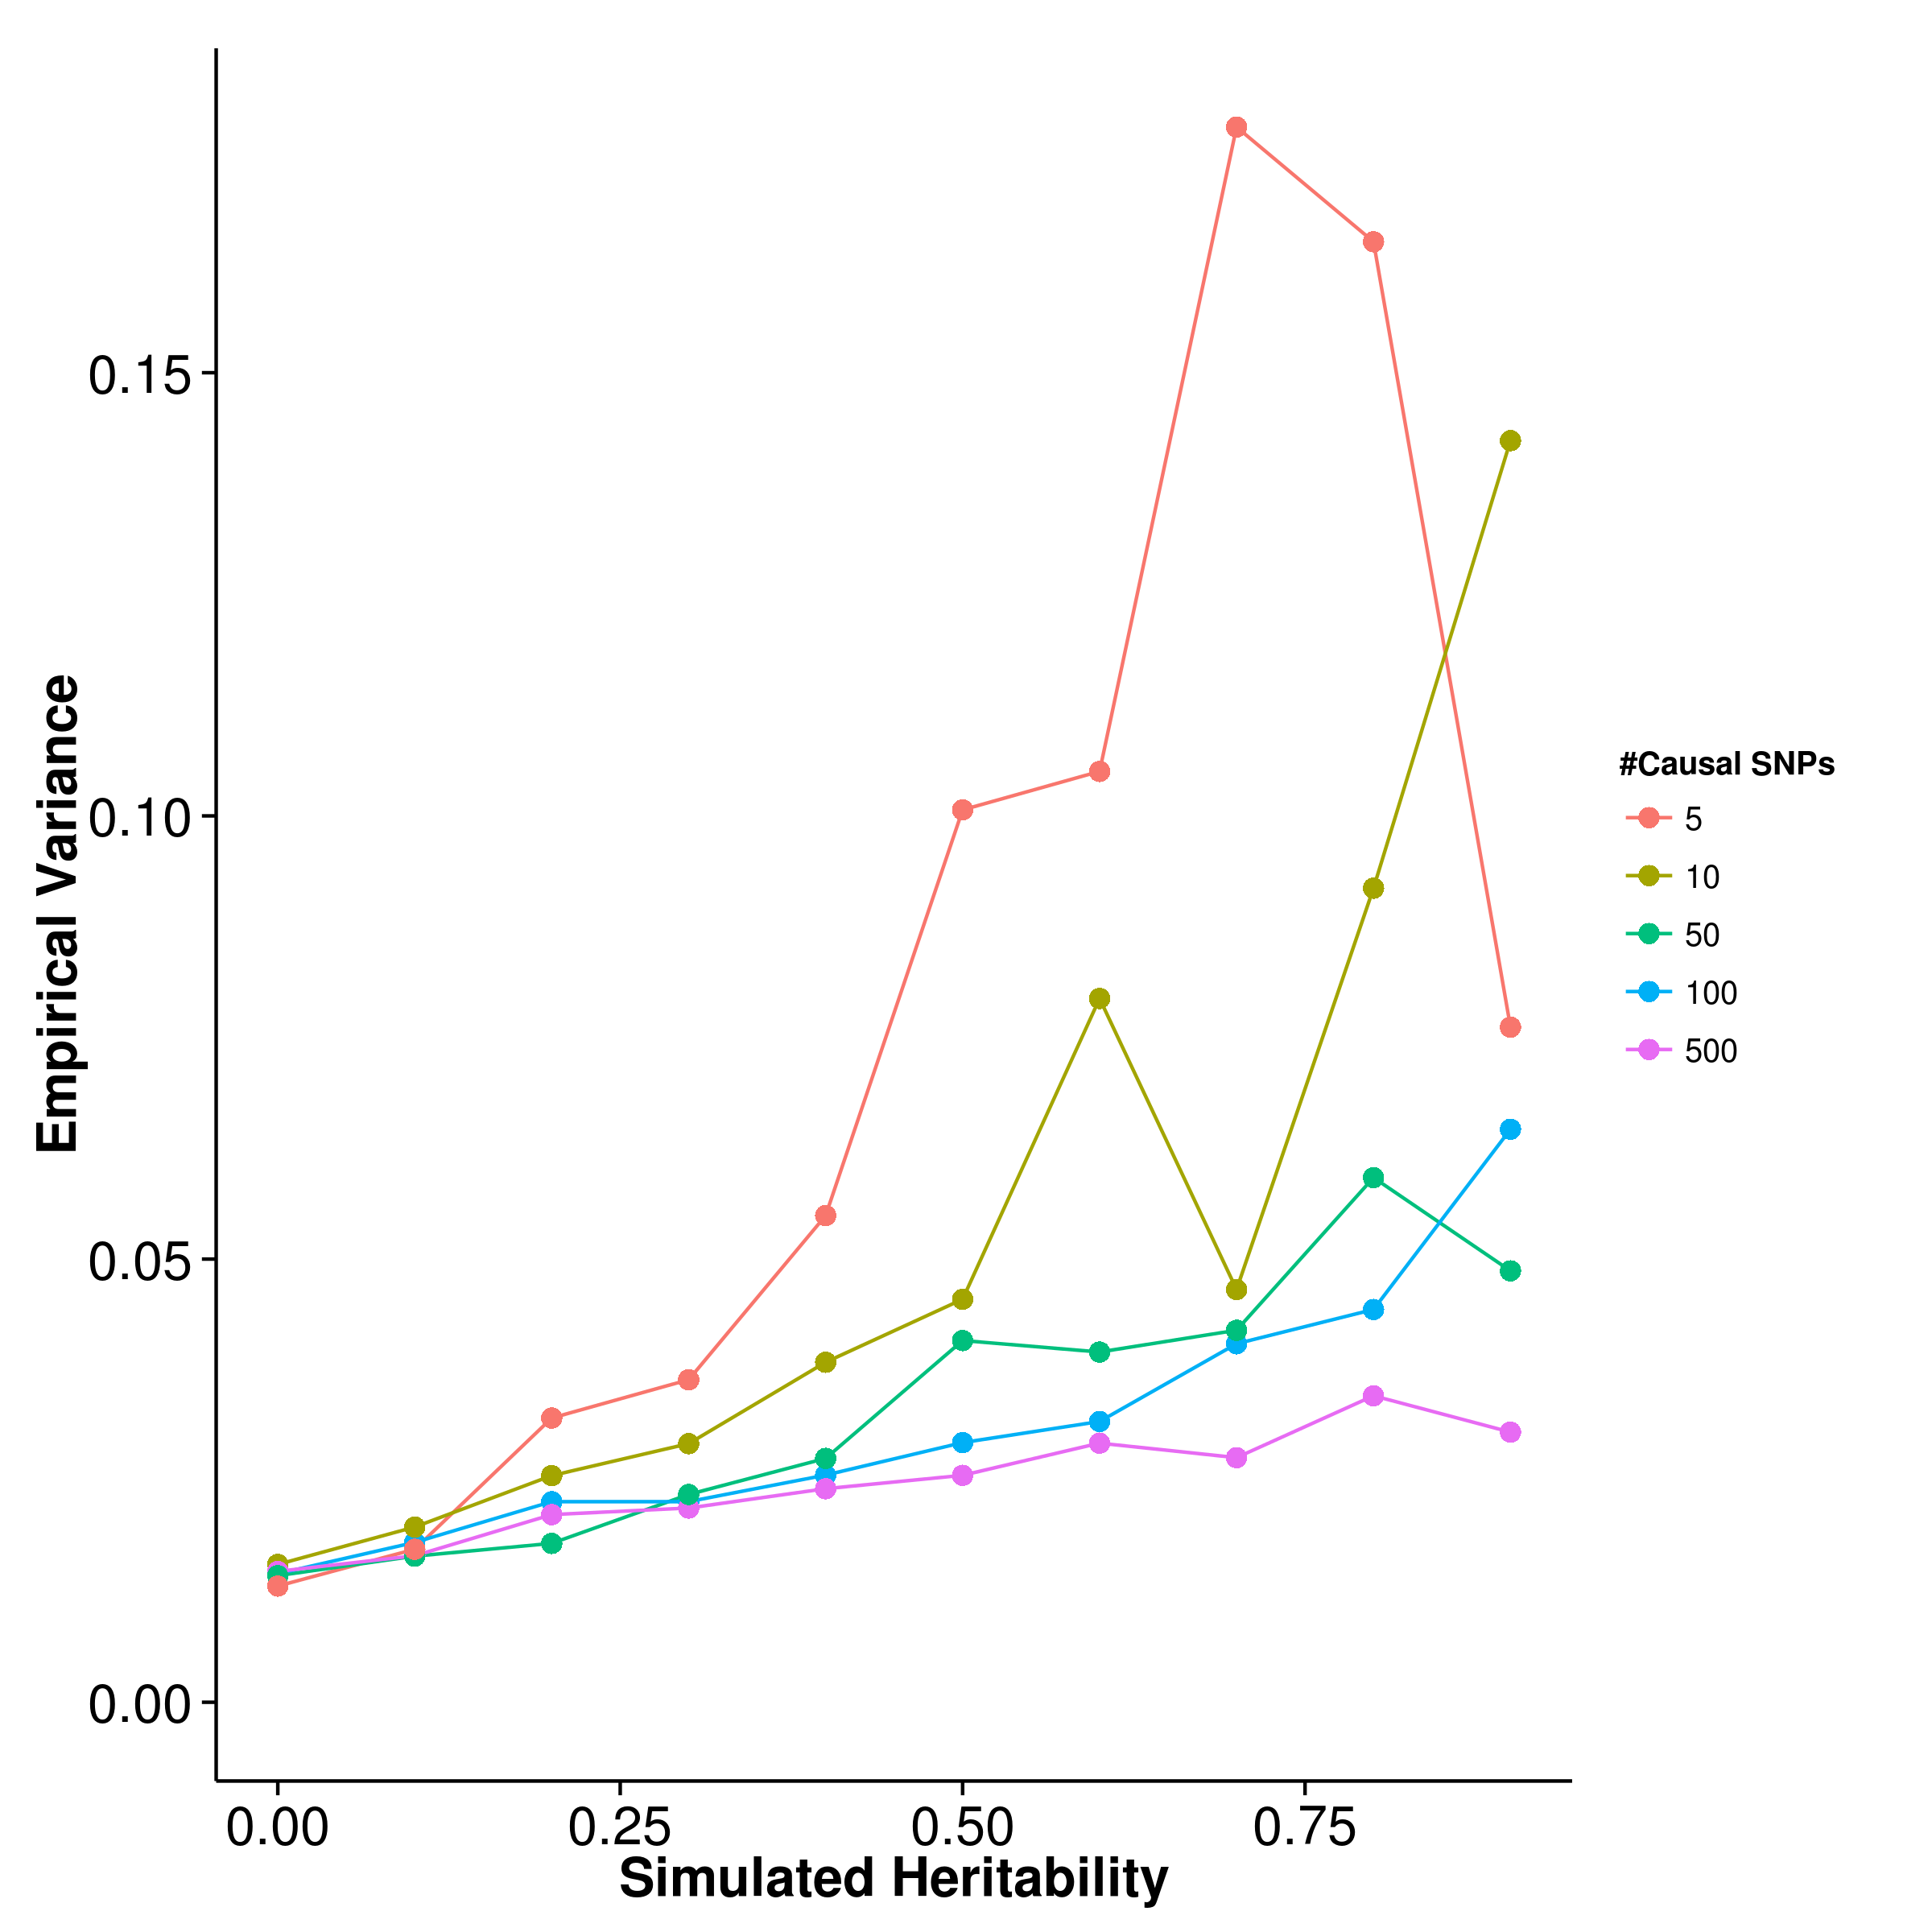
\includegraphics{figure/he_summary/random/ldscIn_Qt_Rand_sd.png}}
					\label{fig:ldscInQtRandVar}
				}
				\caption[Variance of Quantitative Trait Simulation Results]
				{Variance of results from quantitative trait simulation with random effect size simulation.
					Under the polygenic conditions, \gls{gcta} has the smallest variance, follow by \gls{ldsc}. 
					However, it was observed when the number of causal \glspl{SNP} decreases, the variance of the estimation increases for all algorithm, with variance of the \gls{shrek} estimate being the least affected.
					In fact, under oligogenic conditions, \gls{shrek} has a lower empirical variance when compared to \gls{ldsc}.
				} 
				\label{fig:QtRandVar}
			\end{figure}
			%Variance estimate
			\begin{figure}
				\centering
				\subfloat[SHREK]{
					\scalebox{.4}{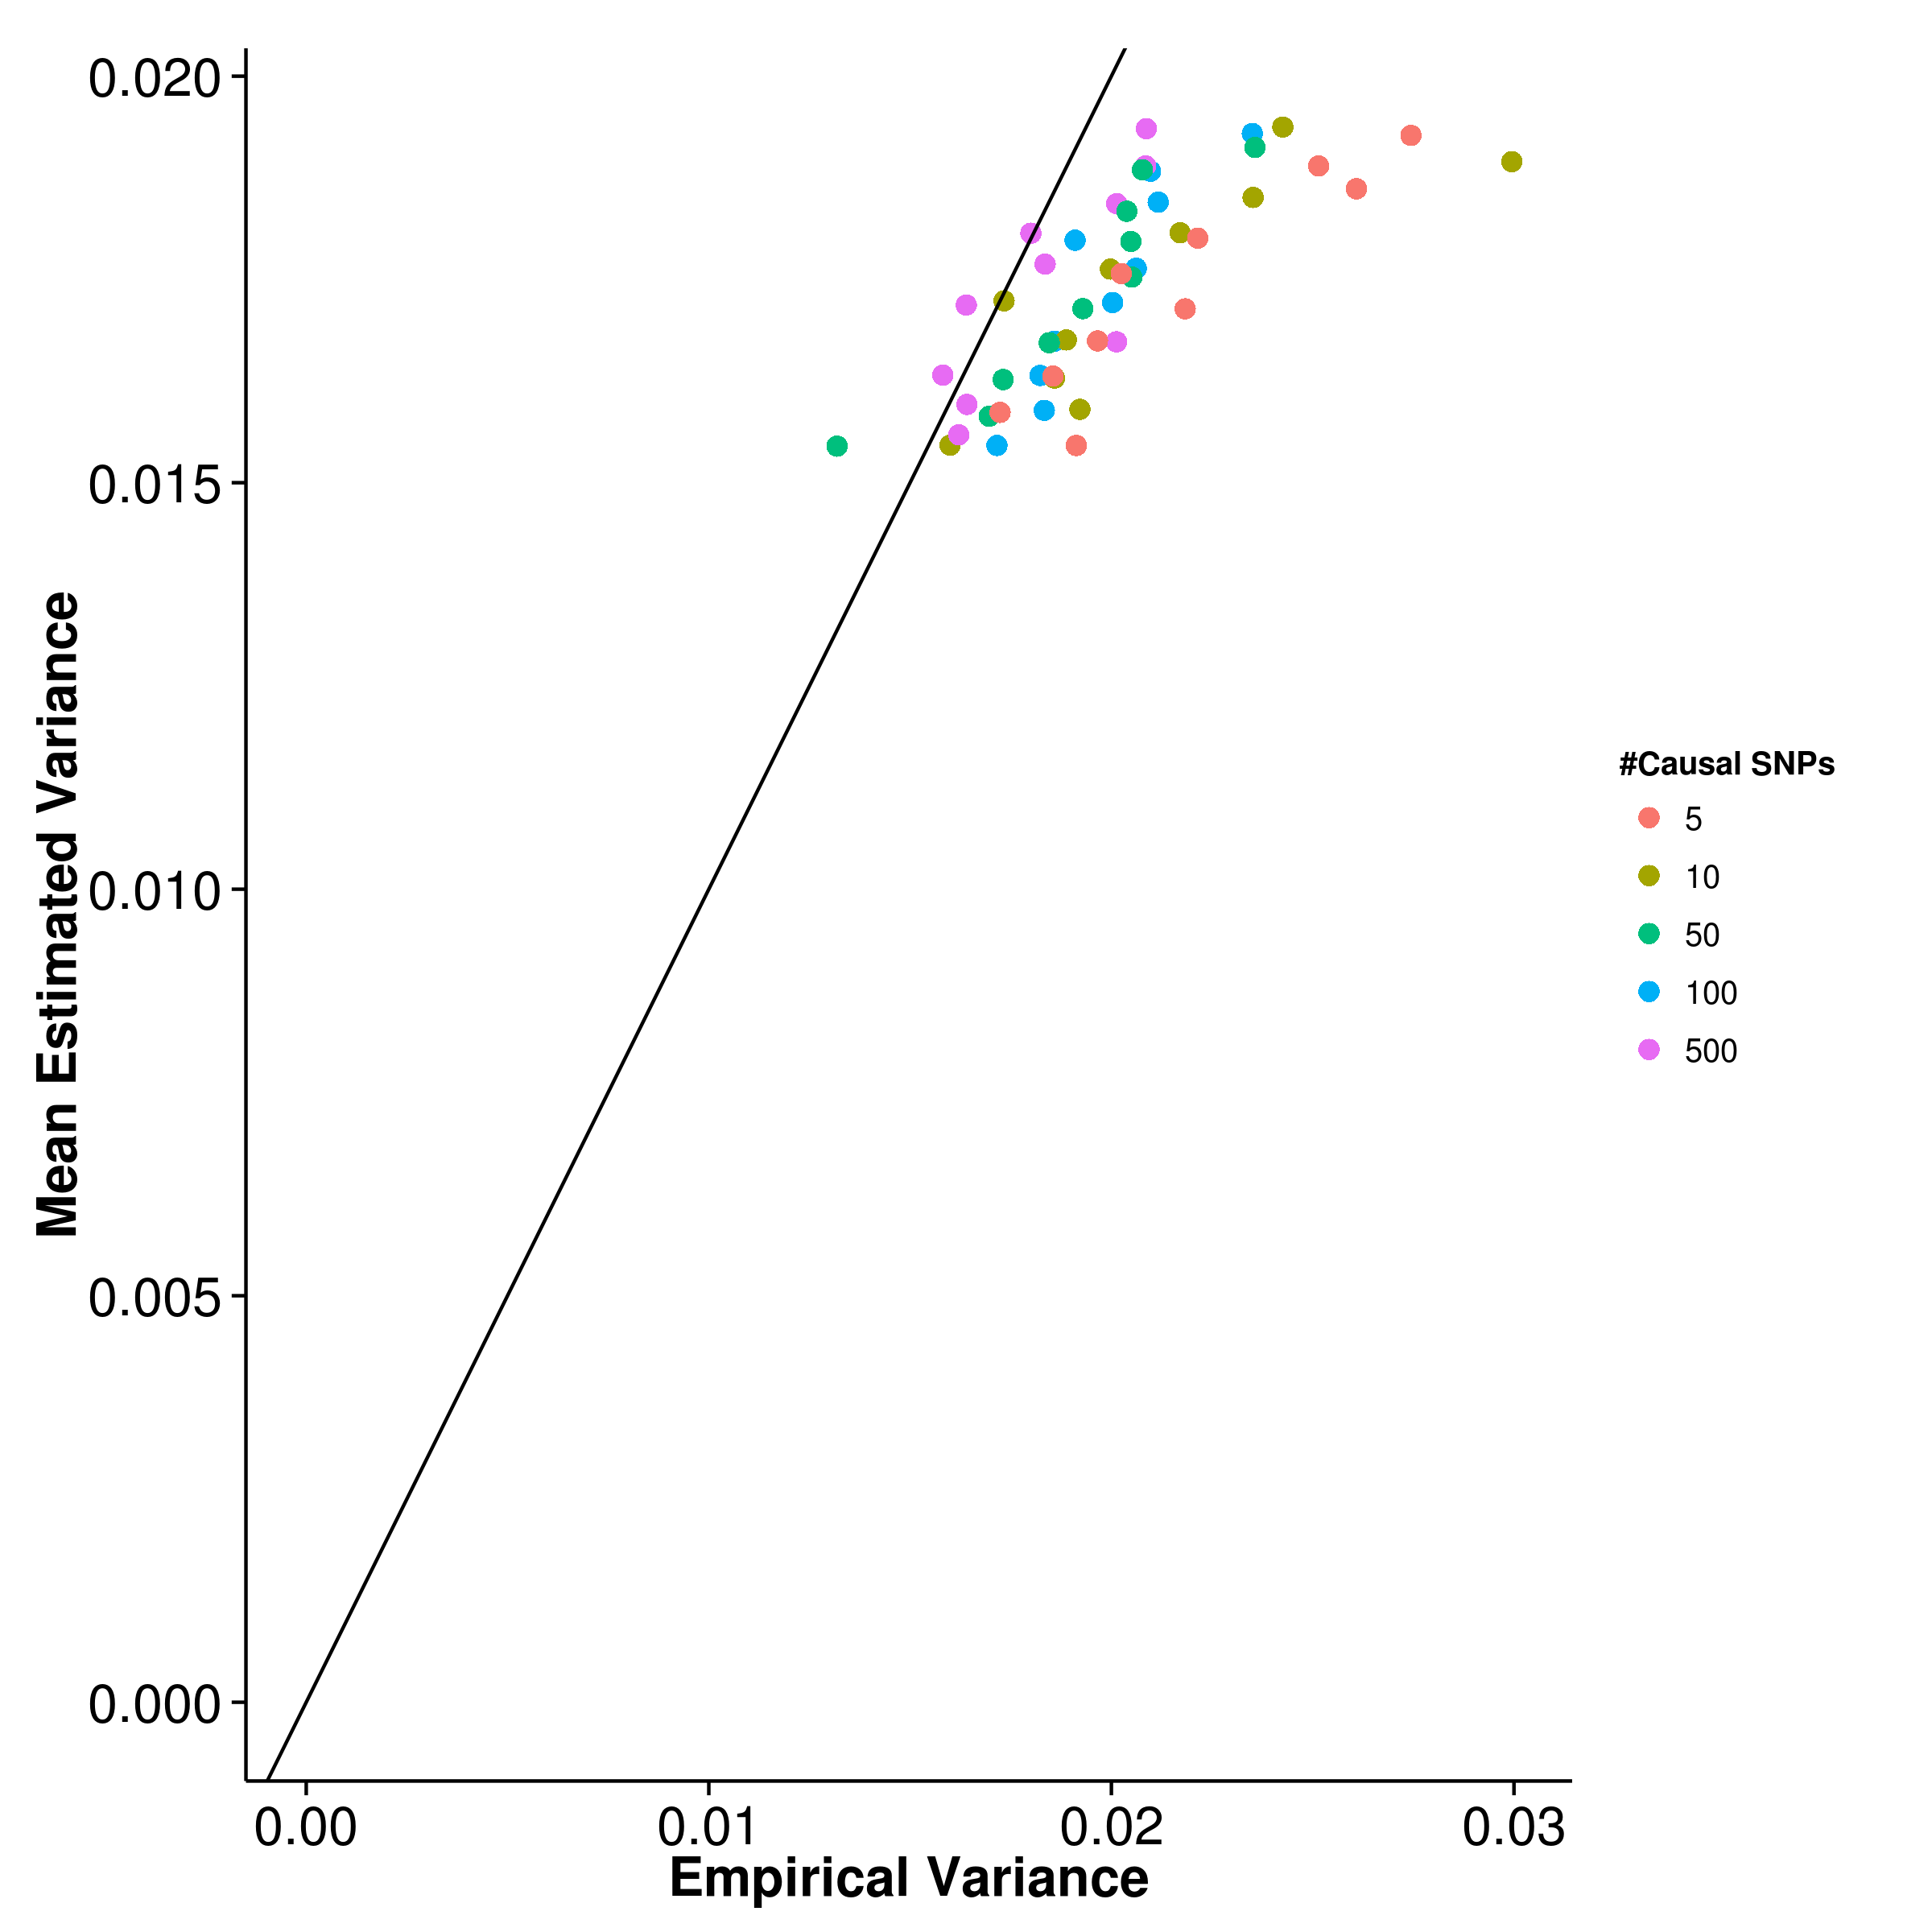
\includegraphics{figure/he_summary/random/shrek_Qt_Rand_sdCom.png}}
					\label{fig:shrekQtRandVarCom}
				}
				\subfloat[GCTA]{
					\scalebox{.4}{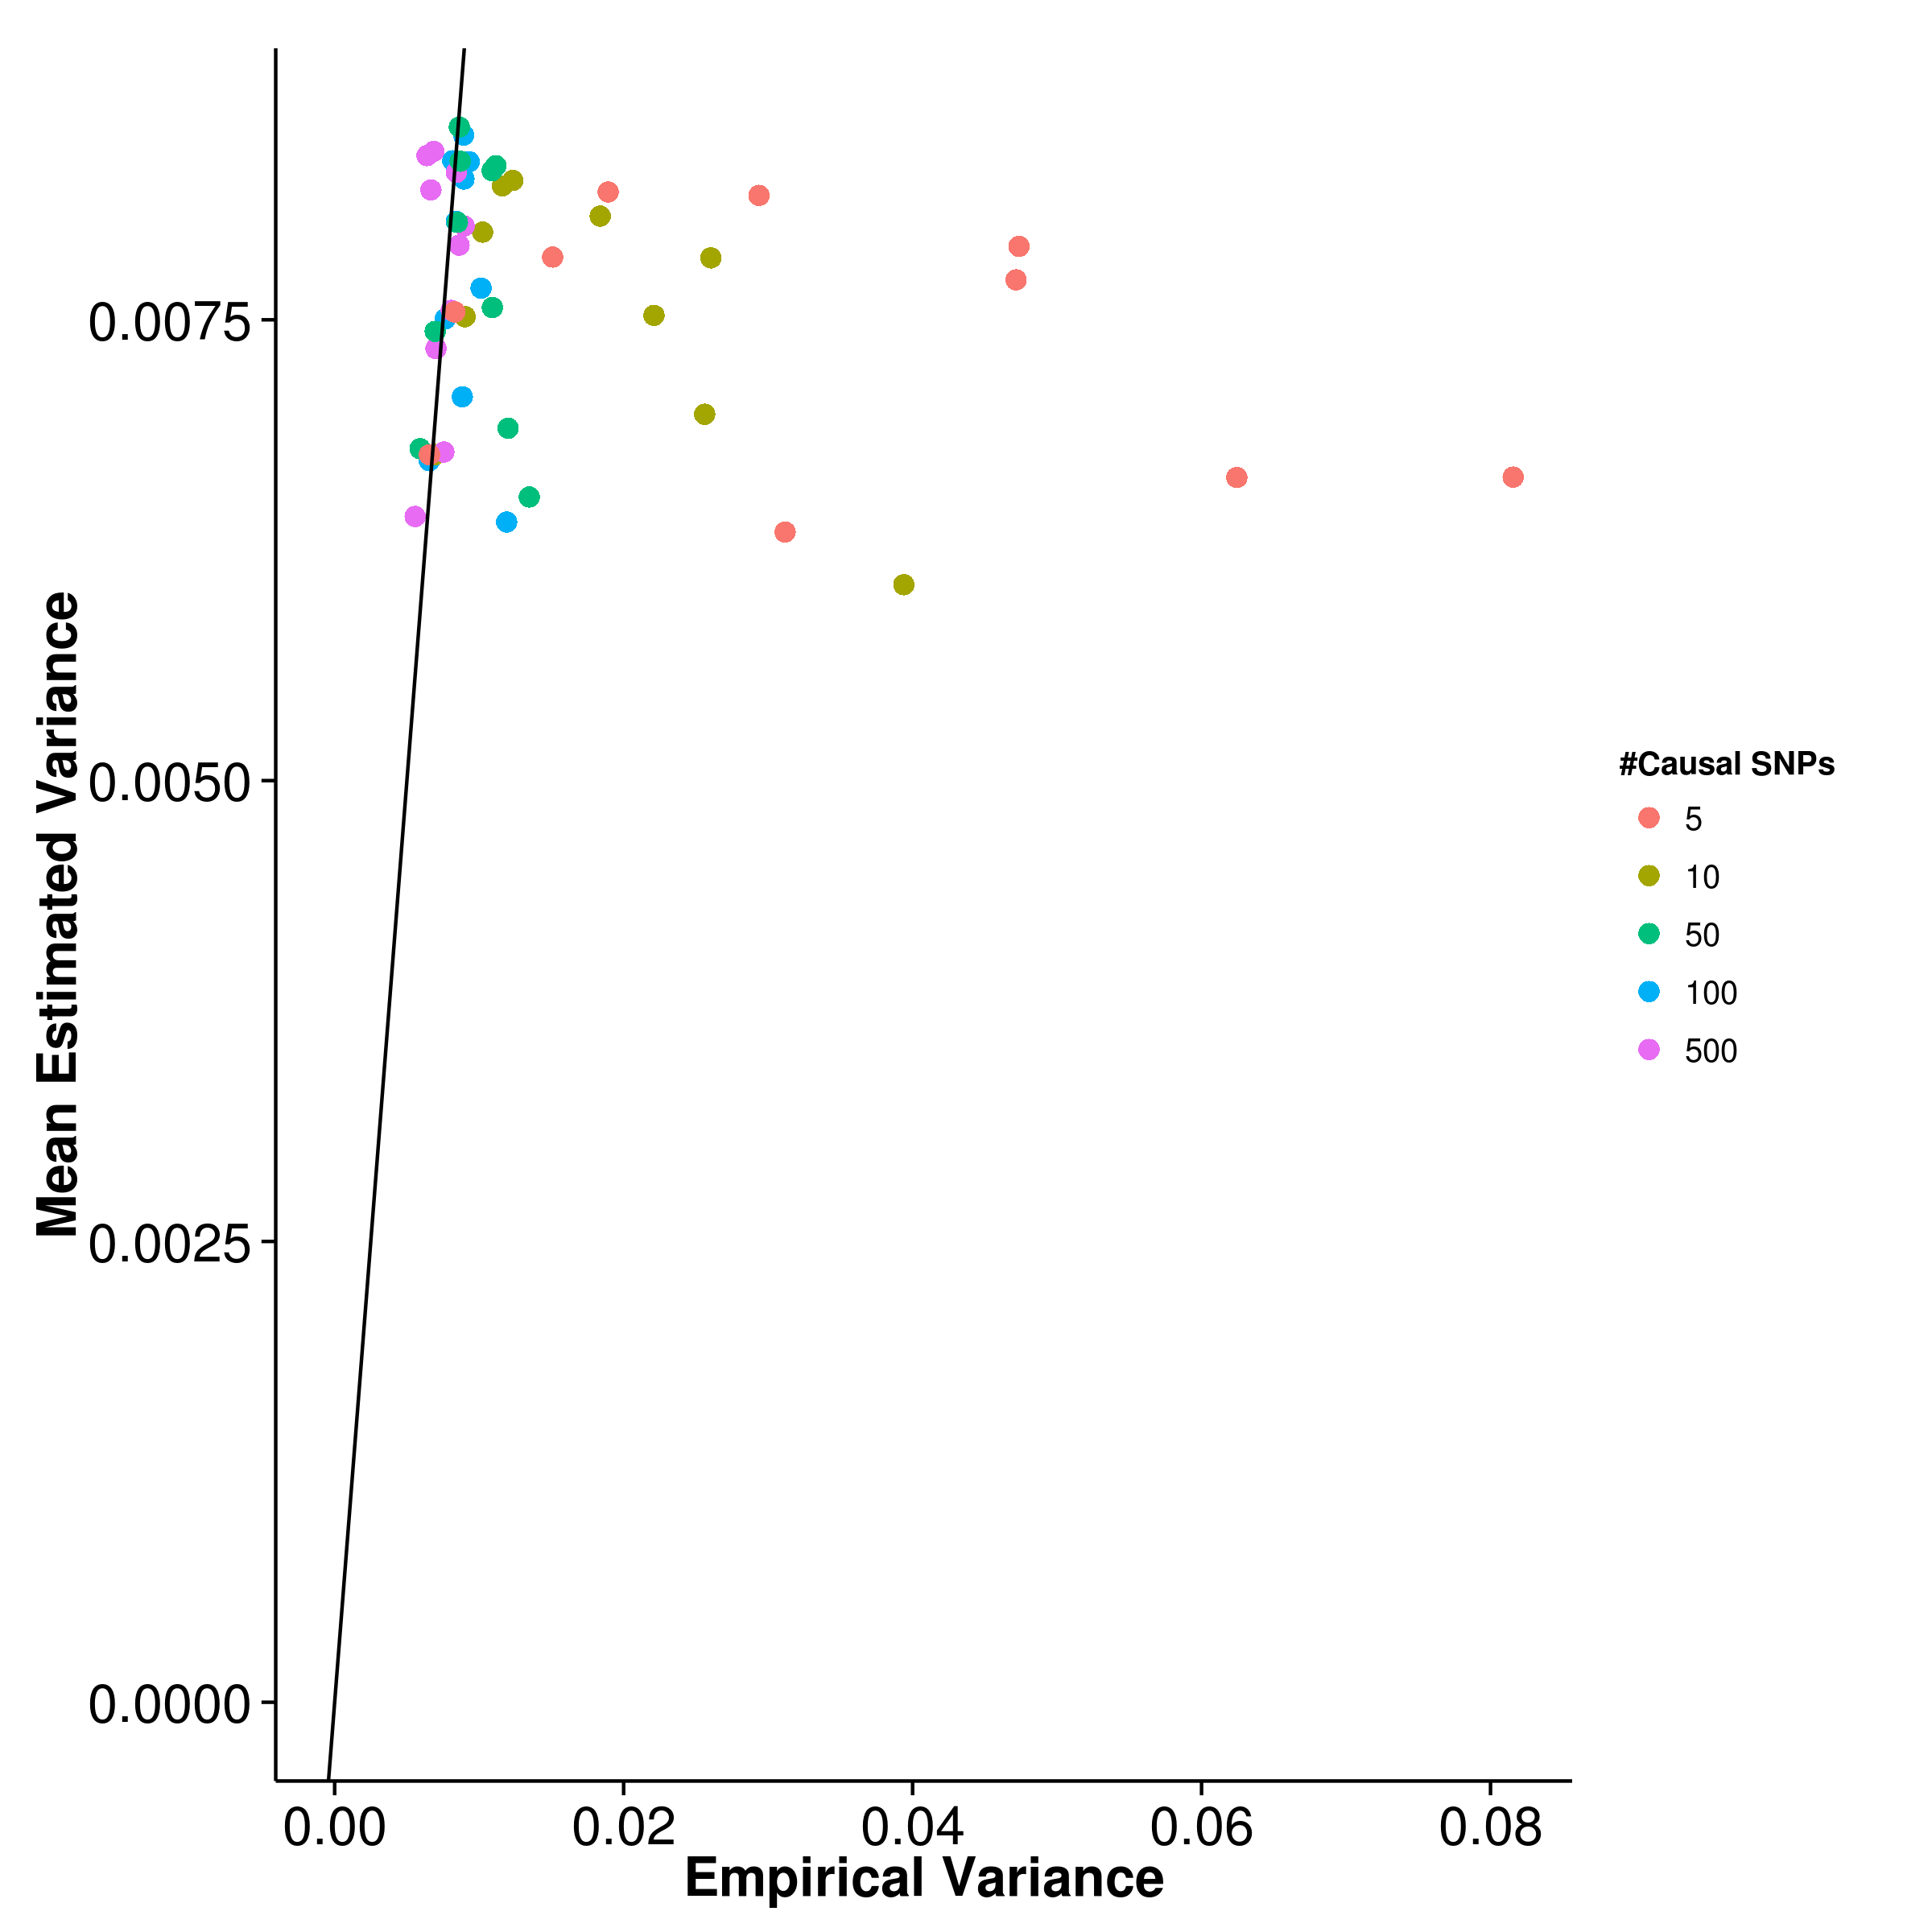
\includegraphics{figure/he_summary/random/gcta_Qt_Rand_sdCom.png}}
					\label{fig:gctaQtRandVarCom}
				}\\
				\subfloat[LDSC with fix intercept]{
					\scalebox{.4}{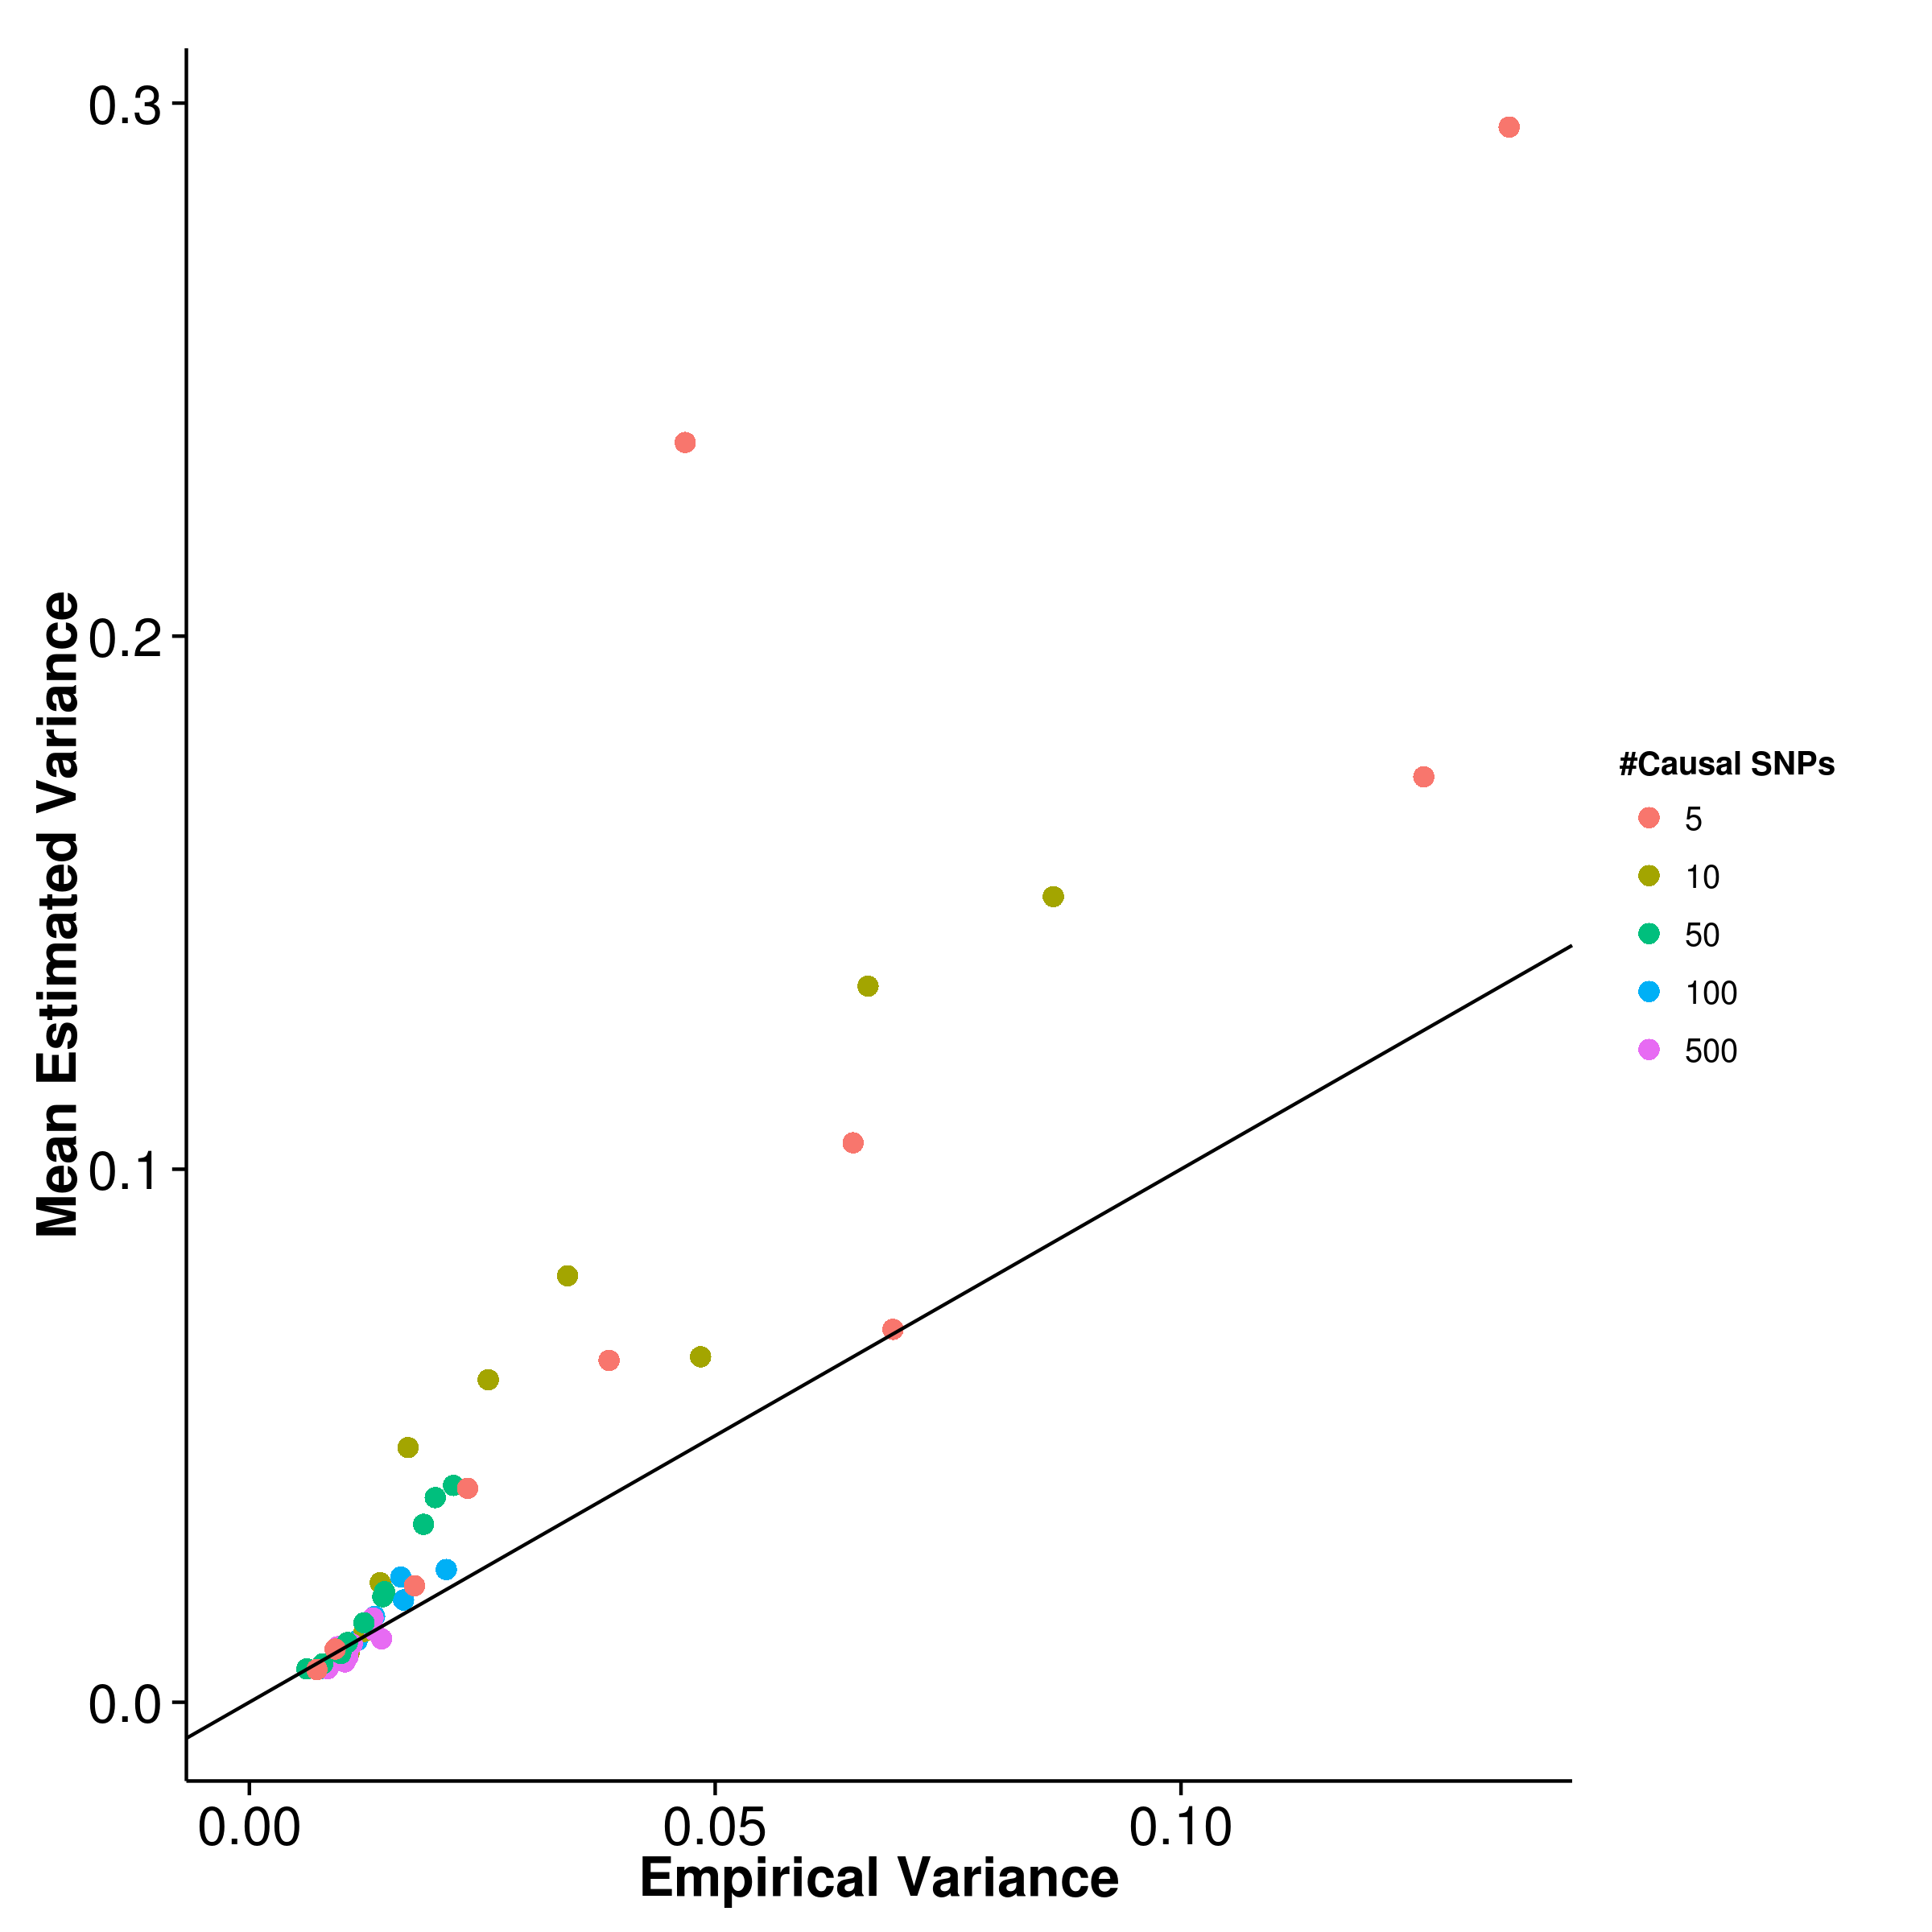
\includegraphics{figure/he_summary/random/ldsc_Qt_Rand_sdCom.png}}
					\label{fig:ldscQtRandVarCom}
				}
				\subfloat[LDSC with intercept estimation]{
					
					\scalebox{.4}{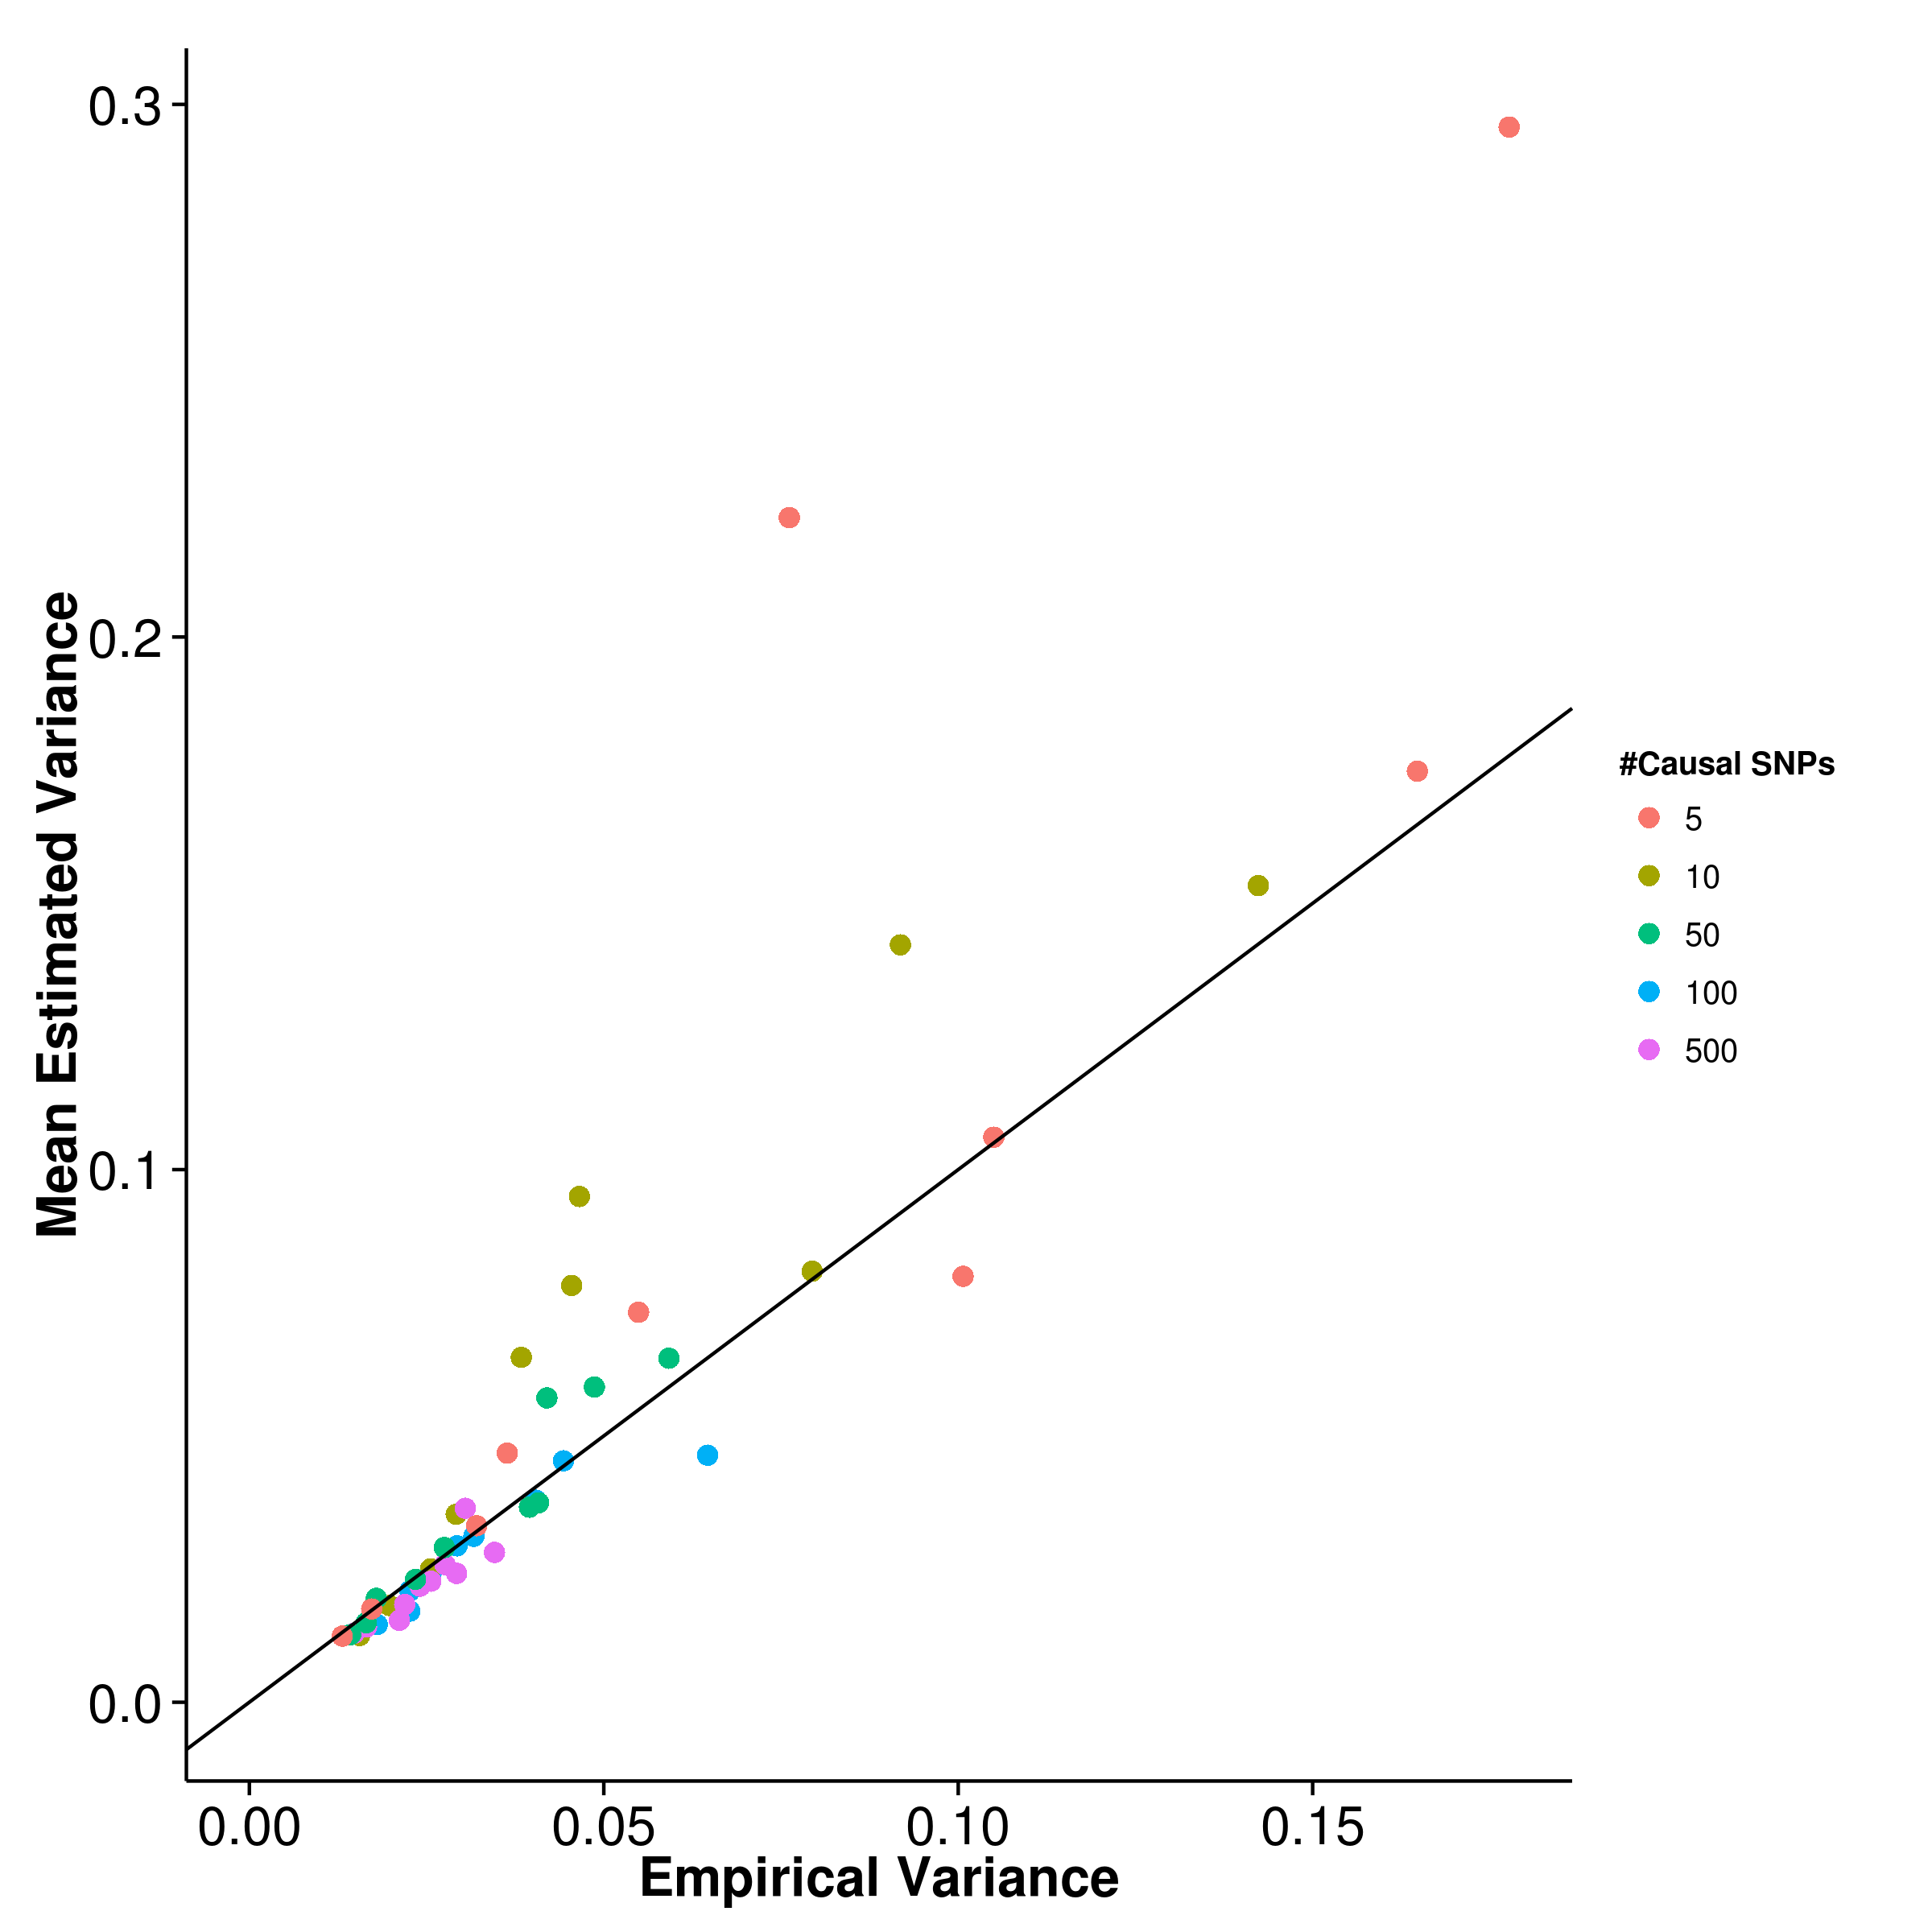
\includegraphics{figure/he_summary/random/ldscIn_Qt_Rand_sdCom.png}}
					\label{fig:ldscInQtRandVarCom}
				}
				\caption[Estimation of Variance in Quantitative Trait Simulation]
				{Estimated variance of results from quantitative trait simulation with random effect size simulation when compared to the empirical variance.
					\gls{gcta} has the best estimate of its empirical variance under the polygenic conditions whereas \gls{shrek} tends to under-estimate its empirical variance.
					On the other hand, \gls{ldsc} tends to over-estimate the variance especially when the number of causal \glspl{SNP} is small.
				} 
				\label{fig:QtRandVarCom}
			\end{figure}
			
		By varying the number of causal \glspl{SNP} and the heritability of the trait, the performance of \gls{ldsc}, \gls{shrek} and \gls{gcta} in the \gls{SNP} heritability estimation of quantitative traits were investigated.
		
		First, when comparing the mean estimates to the simulated heritability, a small upward bias is observed in the estimates from \gls{shrek} (\cref{fig:shrekQtRandMean}).
		On the other hand, estimates from \gls{gcta} are moderately biased downward (\cref{fig:gctaQtRandMean}), similar to the estimates from \gls{ldsc} with intercept estimation (\cref{fig:ldscInQtRandMean}), but with a smaller variability.
		When the intercept was fixed, \gls{ldsc} can accurately estimate the \gls{SNP} heritability.
		And an upward bias can only be observed when the number of \glspl{SNP} is small.
		
		Secondly, the empirical variance of the estimates were also an important indicator of the performance of the algorithms.
		It is clear that empirical variance of the estimates from \gls{ldsc} are sensitive to the number of  causal \glspl{SNP} (\cref{fig:ldscQtRandVar,fig:ldscInQtRandVar}).
		When the number of causal \glspl{SNP} decreases, the variance of the estimates increases, as reported by \citet{Bulik-Sullivan2015}.
		Moreover, consistent with the results from \citet{Bulik-Sullivan2015}, the intercept estimation increases the variance of the estimates from \gls{ldsc}.
		Similarly, although \gls{gcta} has the lowest variance in its estimates, the variance increases when the number of causal \glspl{SNP} decreases  (\cref{fig:gctaQtRandVar}). 
		On the other hand, estimates from \gls{shrek} are relatively insensitive to the number of causal \glspl{SNP}.
		
	\begin{table}
		\centering
		\begin{tabular}{rrrrr}
			\toprule
			Number of Causal SNPs&	SHREK&	LDSC&	LDSC-In&	GCTA \\
			\midrule
			5	&	0.0235	&	0.0576	&	0.0828	&	0.0365\\
			10	&	0.0231	&	0.0343	&	0.0555	&	0.0189\\
			50	&	0.0196	&	0.0157	&	0.0494	&	0.0114\\
			100	&	0.0210	&	0.0129	&	0.0363	&	0.00961\\
			500	&	0.0205	&	0.0115	&	0.0308	&	0.00887\\
			\bottomrule
		\end{tabular}
		\caption[MSE of Quantitative Trait Simulation with Random Effect Size]{
			\Gls{mse} of quantitative trait simulation with random effect size.
			Of all the algorithms, \gls{gcta} has the lowest \gls{mse} except when there is only 5 causal \glspl{SNP}.
			When comparing the performance of \gls{shrek} and \gls{ldsc} with fixed intercept, the performance of \gls{shrek} is better under the oligogenic condition whereas \gls{ldsc} with fixed intercept excels under the polygenic condition. 
			On the other hand, when intercept estimation were performed, the \gls{mse} of \gls{ldsc} increases, mainly due to the increased \gls{se}. 
			Therefore \gls{shrek} outperforms \gls{ldsc} with intercept estimation when there are minimal confounding variables.
		}
		\label{tab:mseQtRandom}
	\end{table}
		Finally, it is equally important for the algorithms to be able to estimate the variance of its estimates.
		It is observed that when the number of causal \glspl{SNP} is large, \gls{gcta} can accurately estimates its variance (\cref{fig:gctaQtRandVarCom}).
		However, when the number of causal \glspl{SNP} decreases, \gls{gcta} underestimates the variance of its estimates. 
		On the other hand, \gls{shrek} consistently underestimate the variance of its estimates (\cref{fig:shrekQtRandVarCom}).
		But when compared to \gls{ldsc}, the magnitude of bias of the variance estimated from \gls{shrek} is much smaller.
		\gls{ldsc} tends to overestimate its variance (\cref{fig:ldscQtRandVarCom,fig:ldscInQtRandVarCom}), and only when the intercept estimation was performed can \gls{ldsc} has a better estimates of the variance when the number of causal \glspl{SNP} is large. 
		
		Taking into account of the bias and variance of the estimates, \gls{gcta} has the best overall performance.
		On the other hand, when the number of causal \glspl{SNP} is small, \gls{shrek} has a better performance when compared to \gls{ldsc}, whereas \gls{ldsc} performs better under polygenic condition.
		It is also observed that estimates from \gls{shrek} is the least sensitive to changes in the genetic architecture among the algorithms tested (\cref{tab:mseQtRandom}).  
		
		\subsubsection{Quantitative Trait Simulation with Extreme Effect Size}
		%Mean
		\begin{figure}
			\centering
			\subfloat[SHREK]{
				\scalebox{.4}{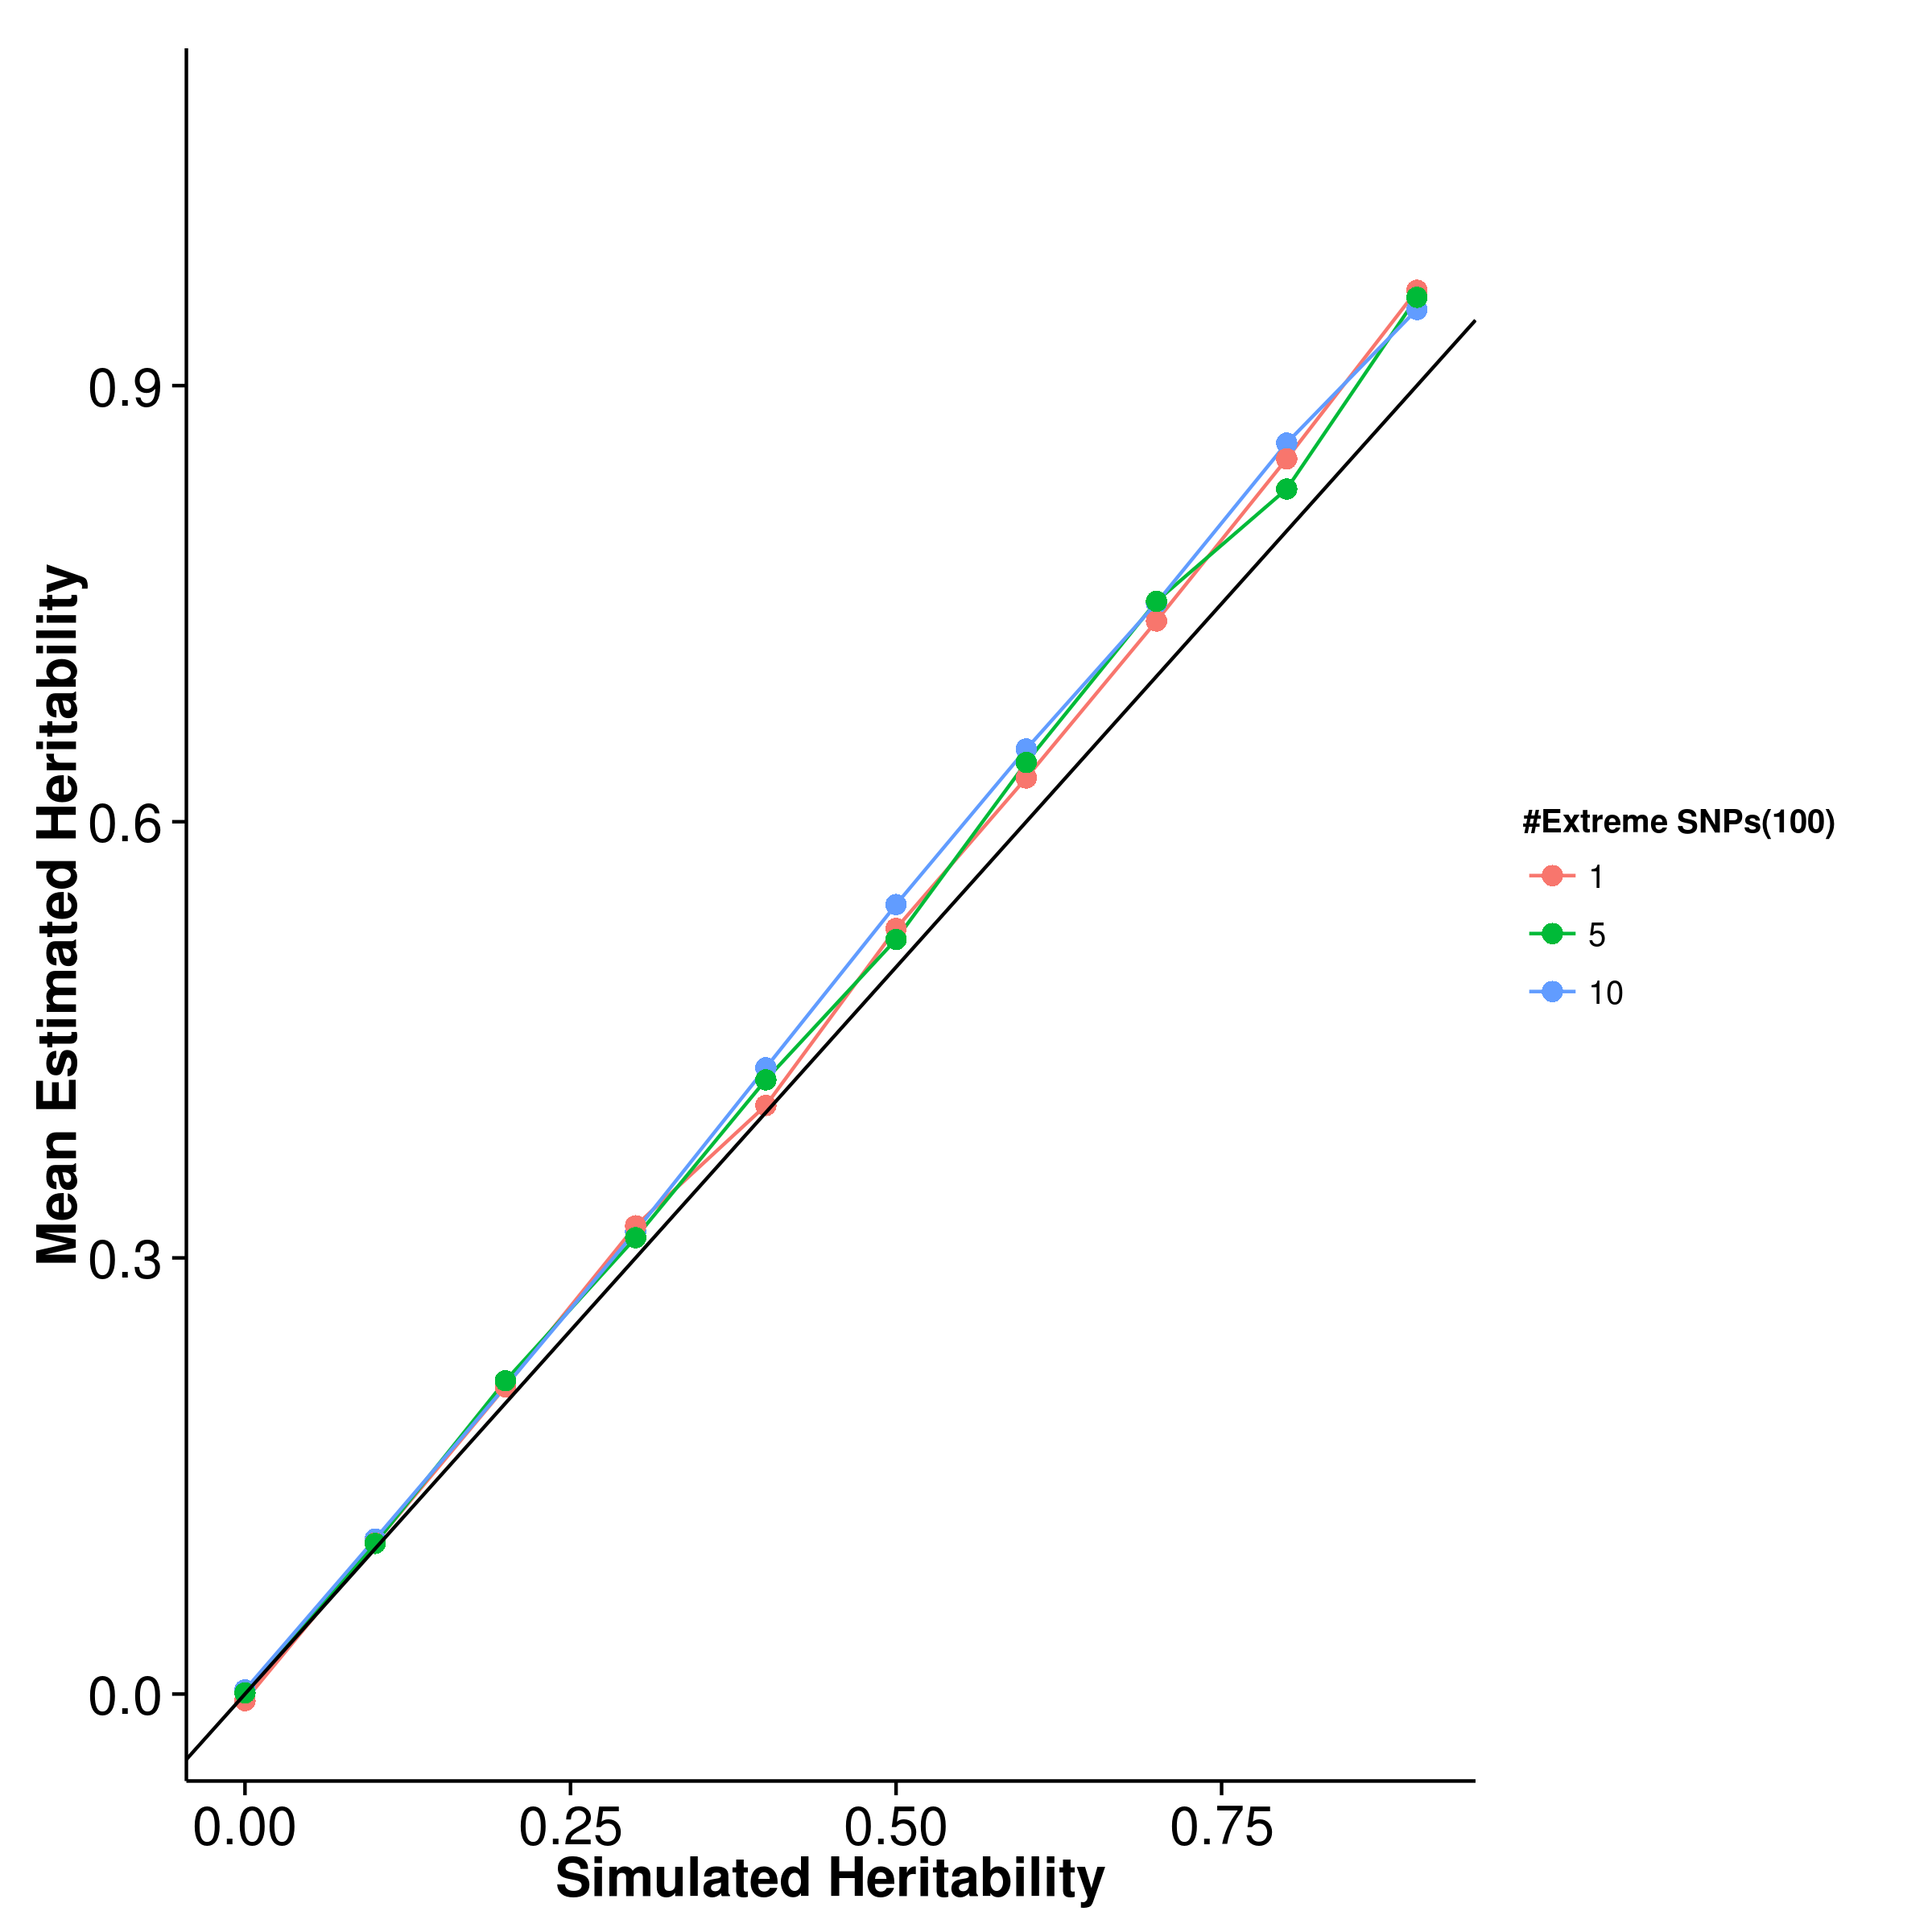
\includegraphics{figure/he_summary/extreme_100c/shrek_QtE_Rand_mean.png}}
				\label{fig:shrekQtEx100cMean}
			}
			\subfloat[GCTA]{
				\scalebox{.4}{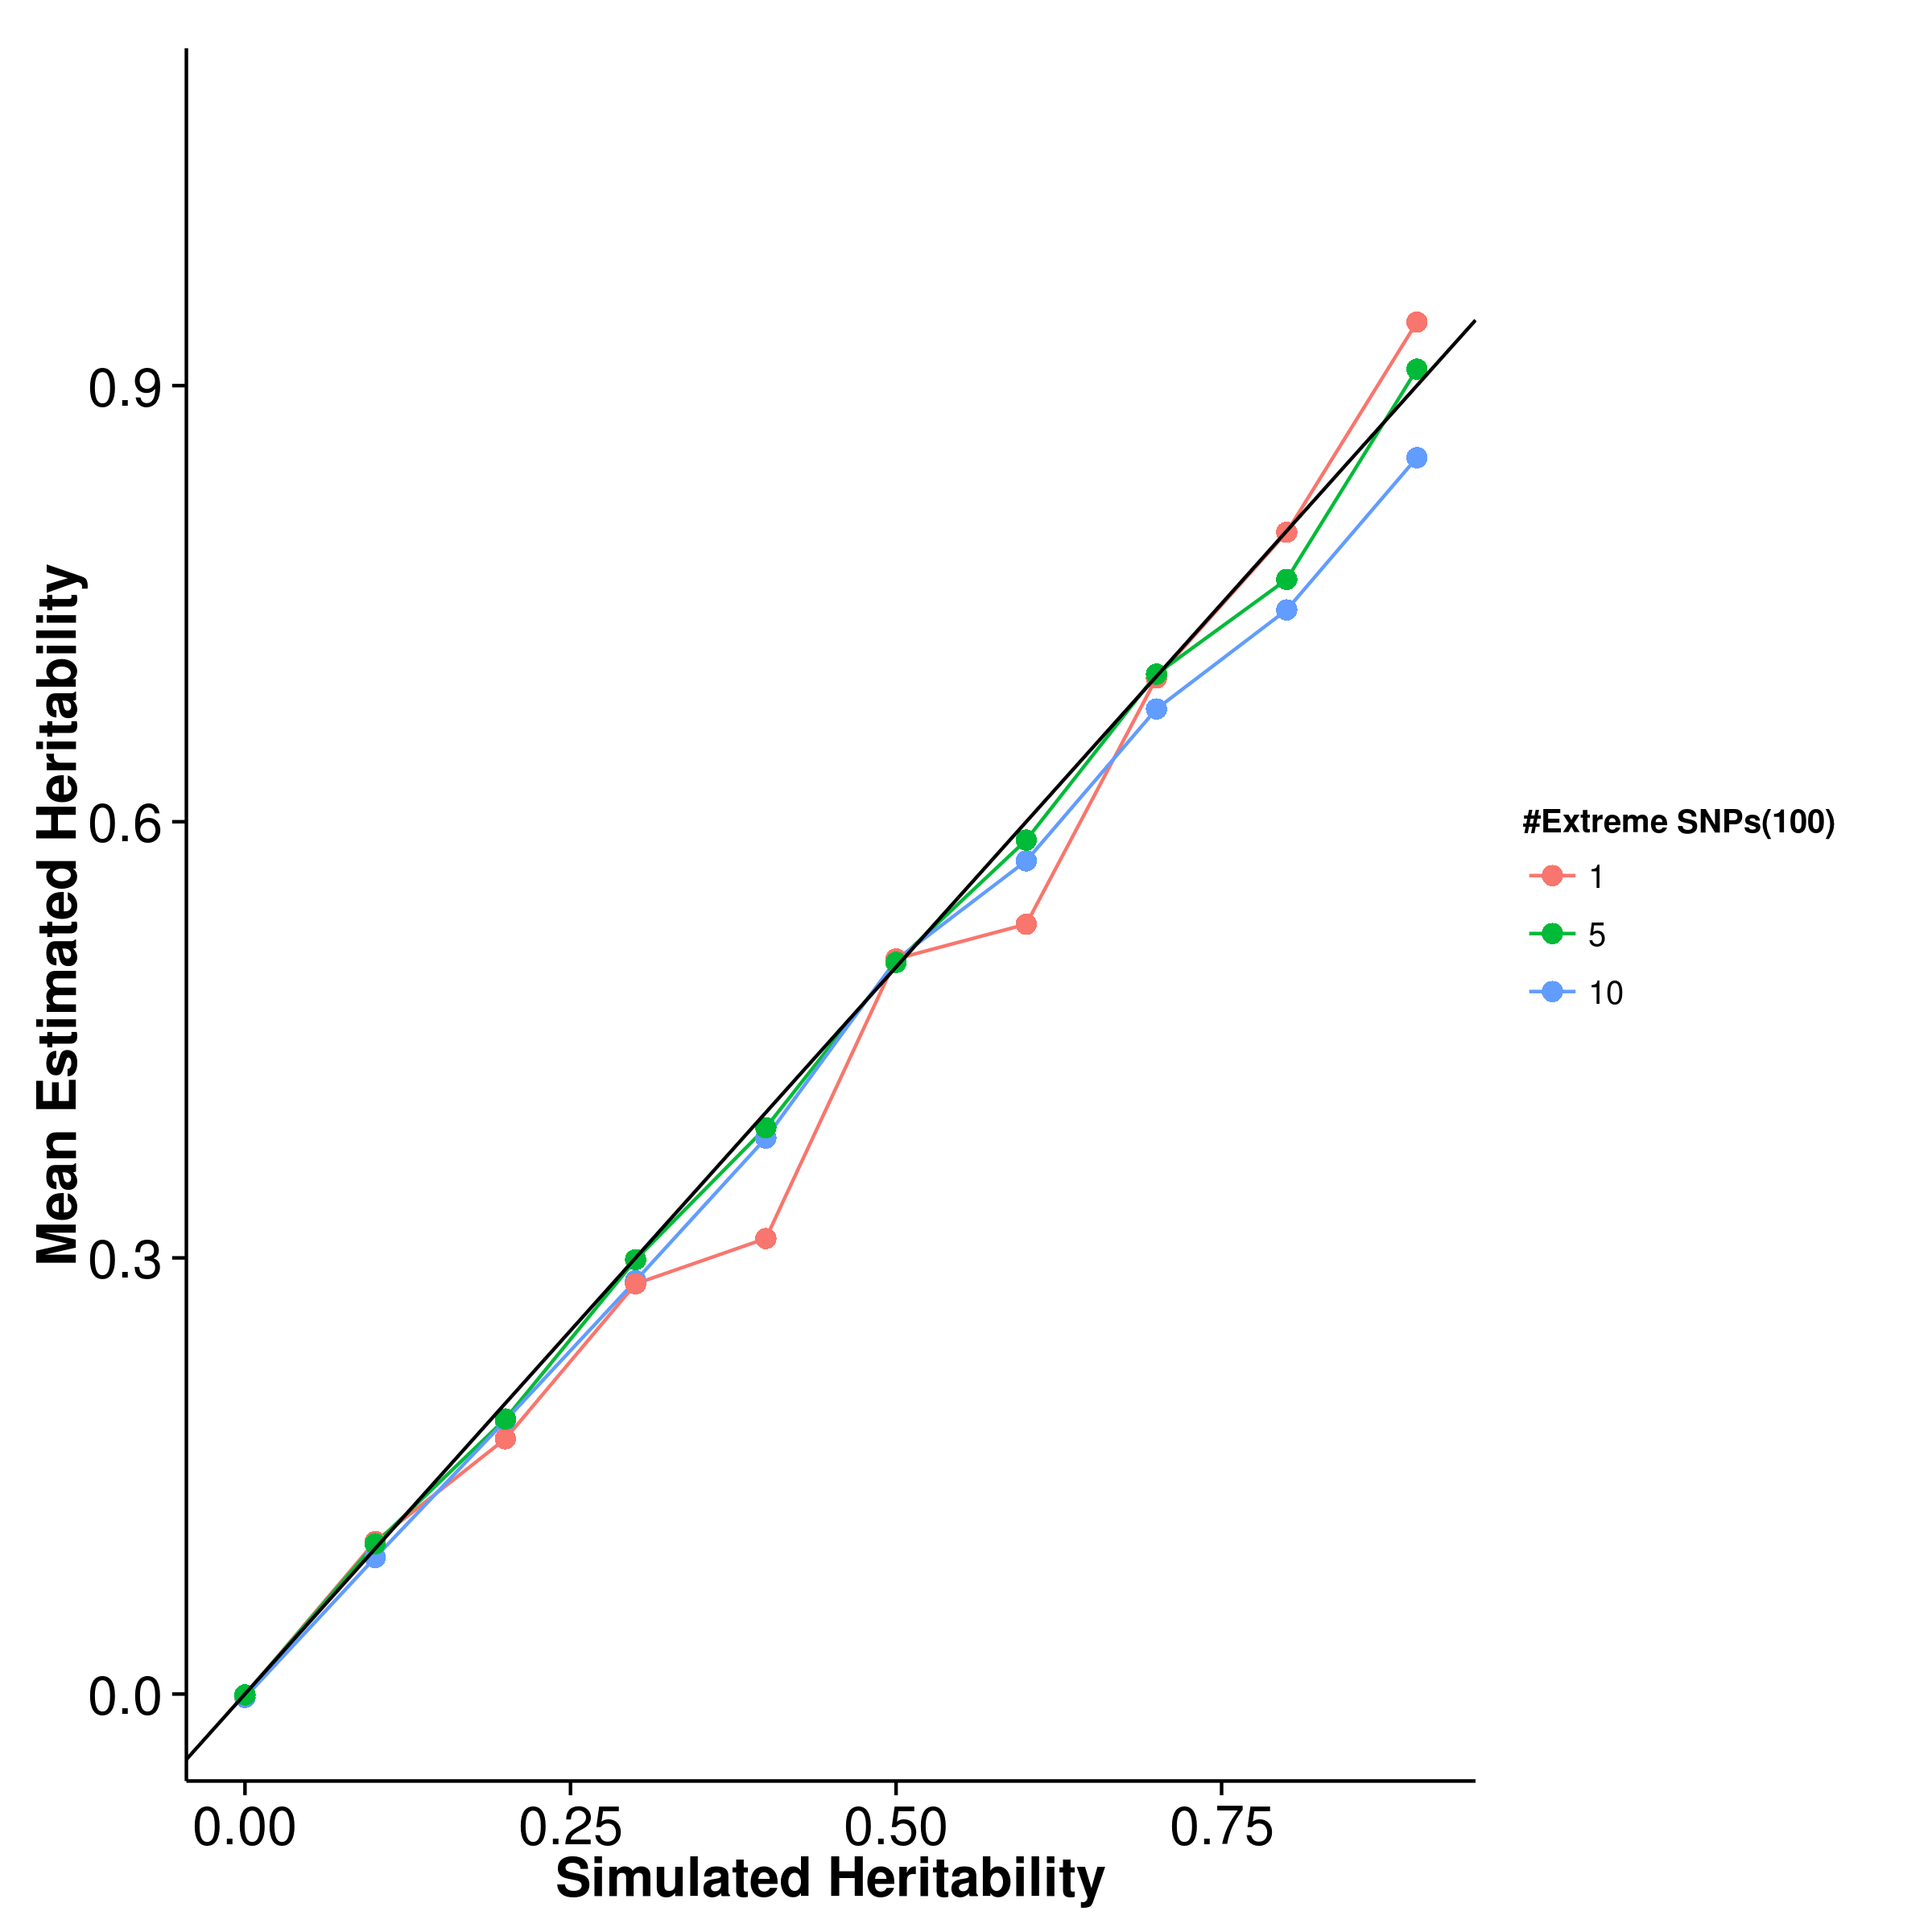
\includegraphics{figure/he_summary/extreme_100c/gcta_QtE_Rand_mean.png}}
				\label{fig:gctaQtEx100cMean}
			}\\
			\subfloat[LDSC with fix intercept]{
				\scalebox{.4}{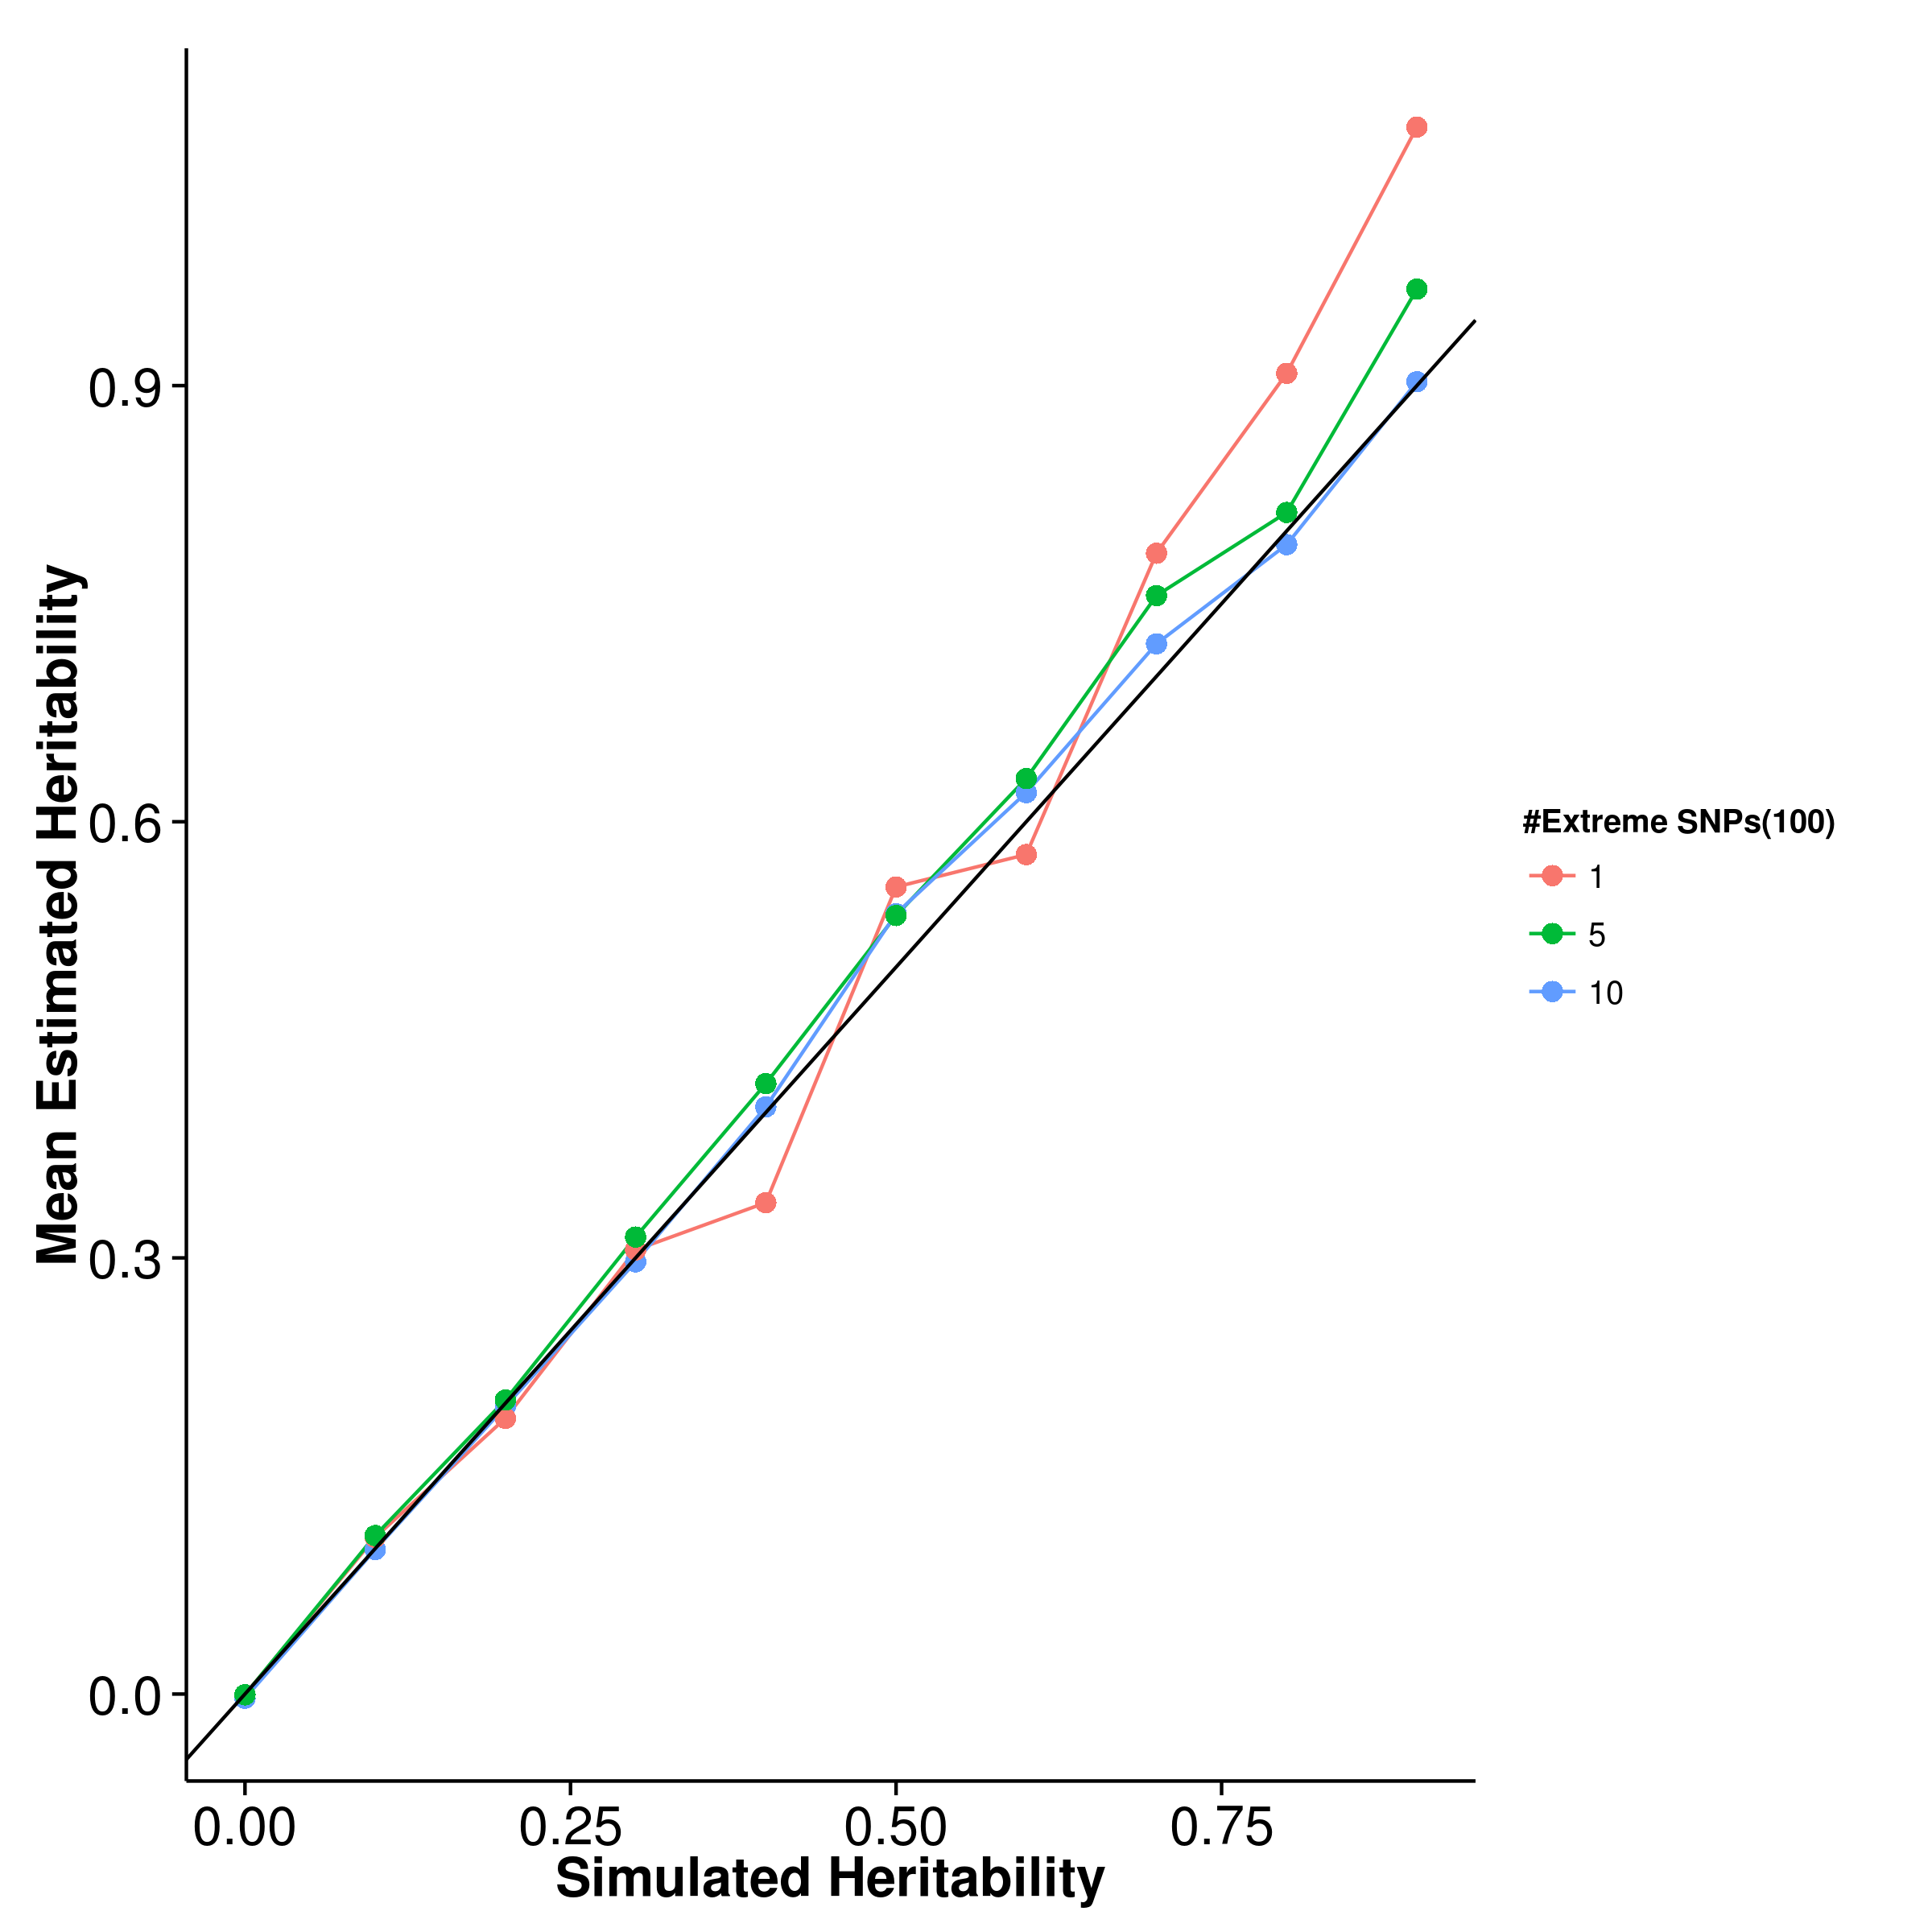
\includegraphics{figure/he_summary/extreme_100c/ldsc_QtE_Rand_mean.png}}
				\label{fig:ldscQtEx100cMean}
			}
			\subfloat[LDSC with intercept estimation]{
				
				\scalebox{.4}{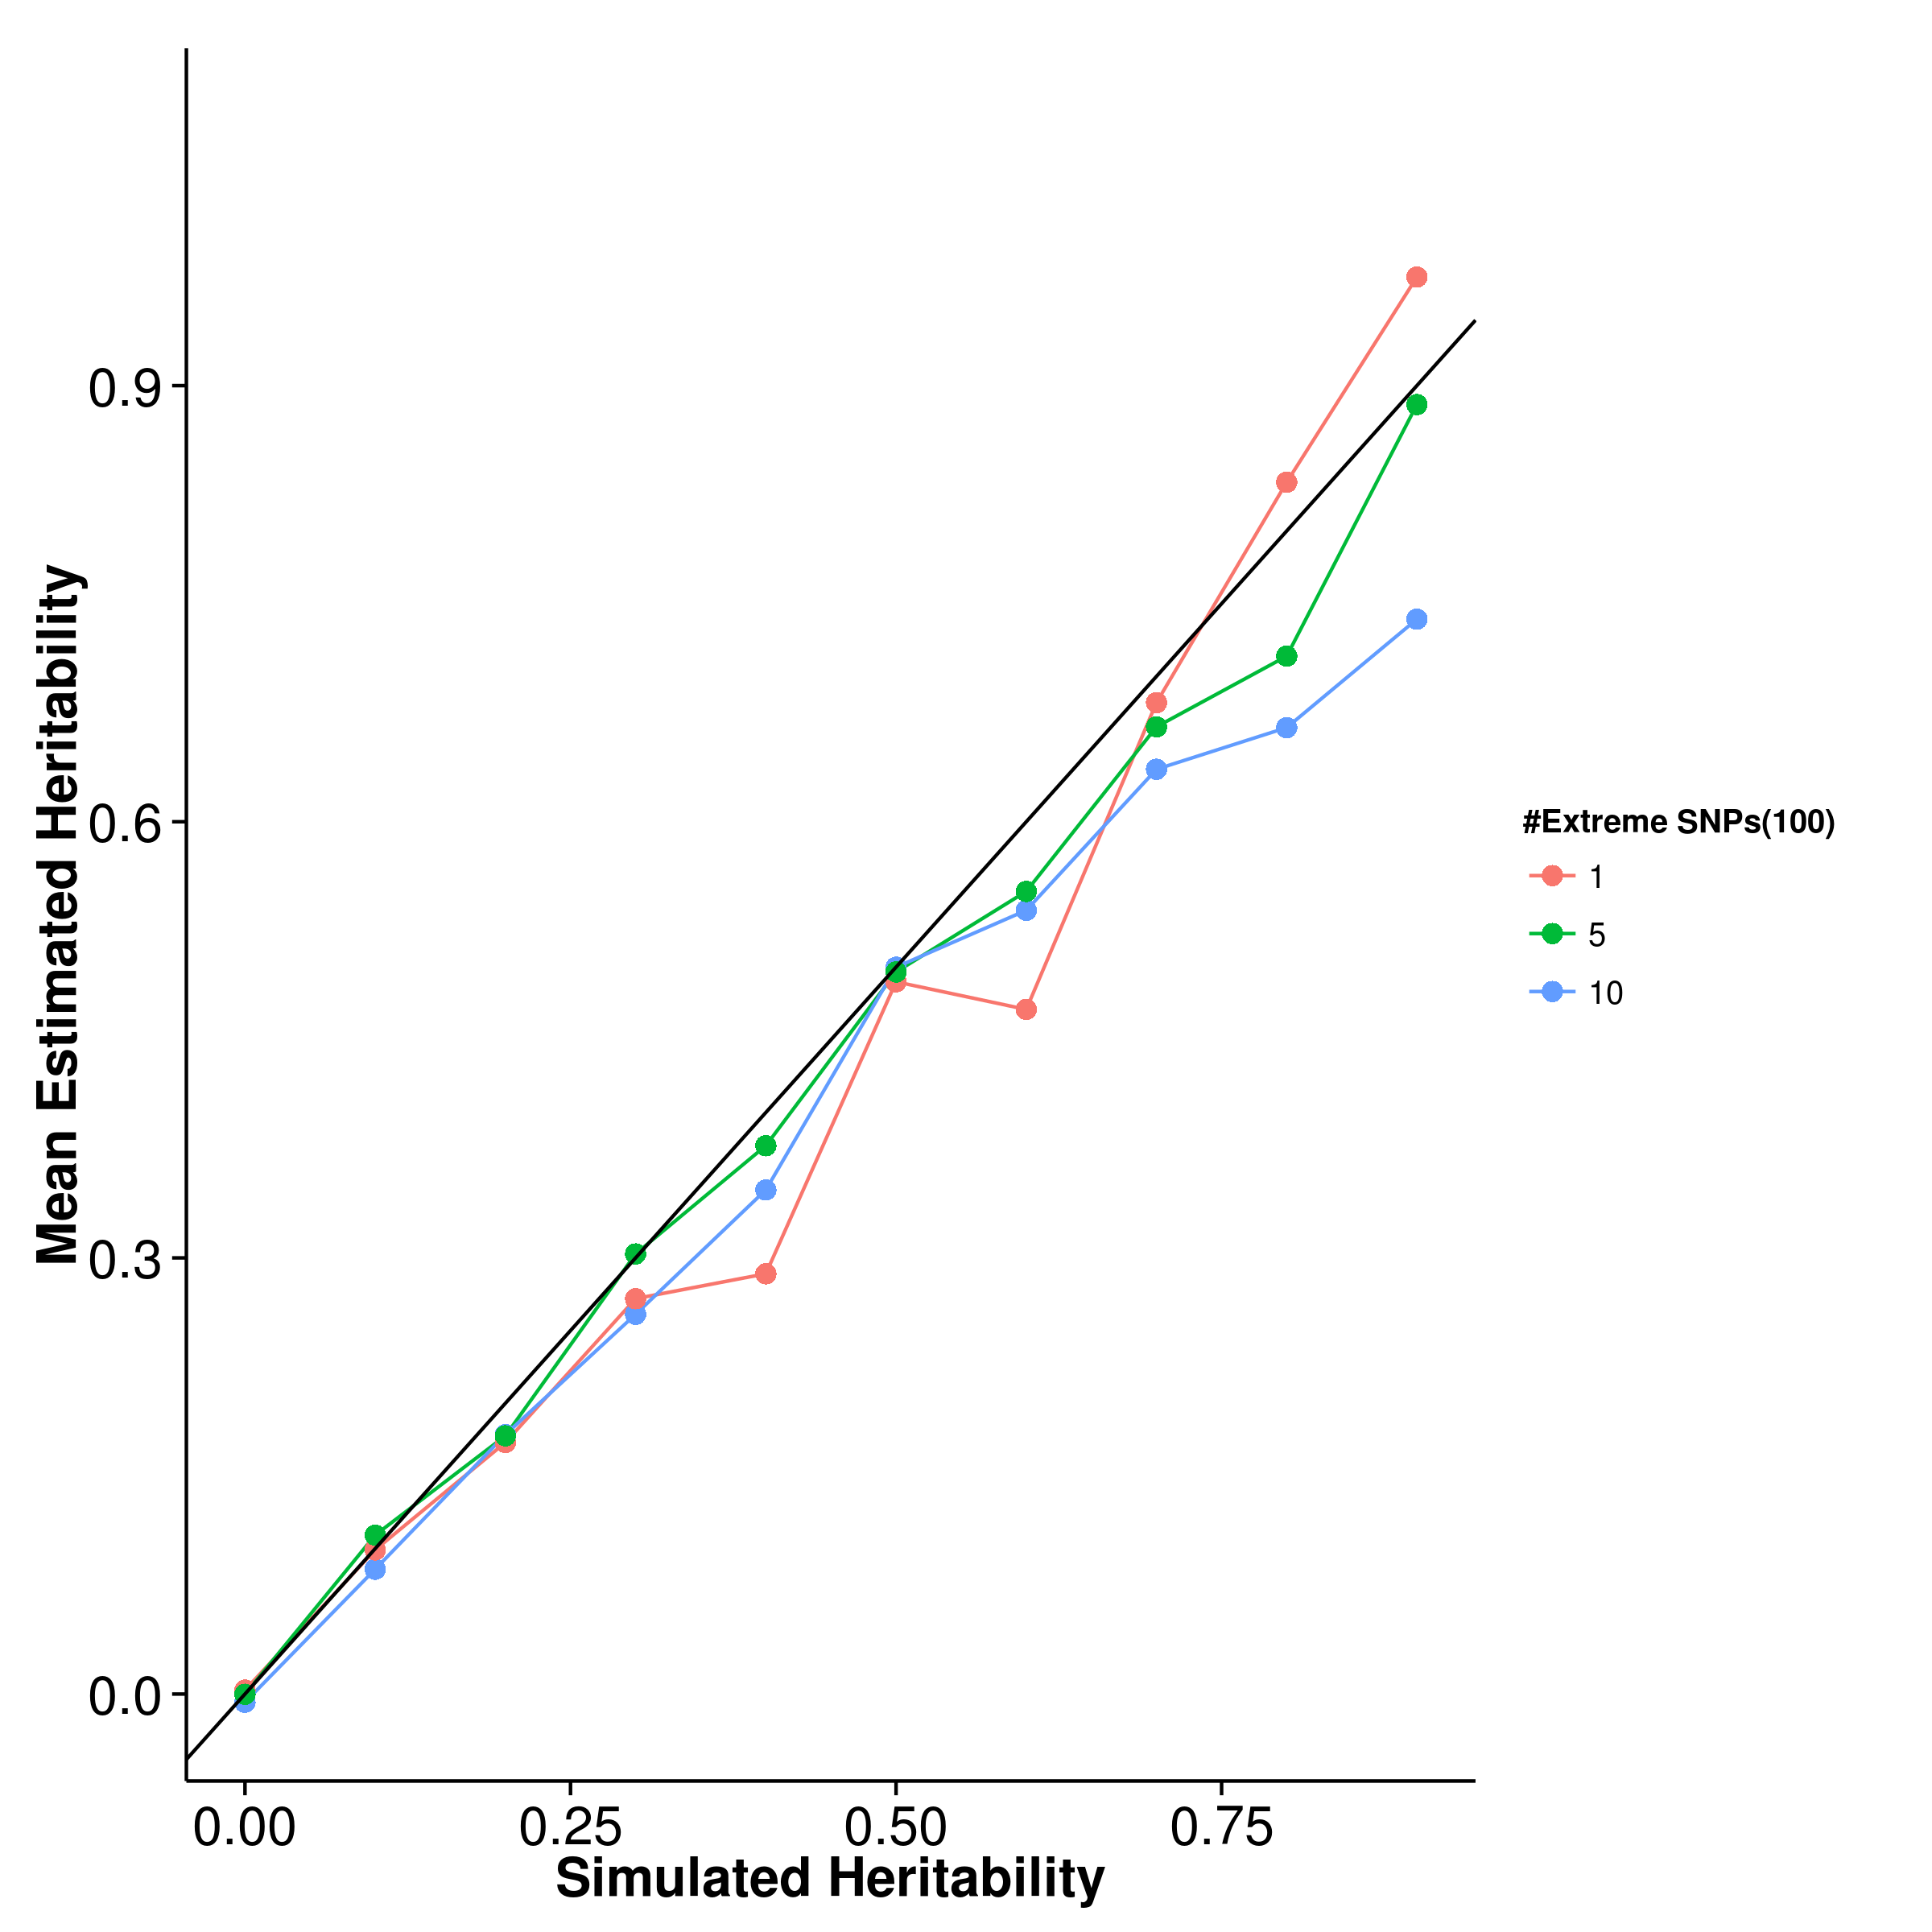
\includegraphics{figure/he_summary/extreme_100c/ldscIn_QtE_Rand_mean.png}}
				\label{fig:ldscInQtEx100cMean}
			}
			\caption[Mean of Extreme Effect Size Simulation Result]
			{Mean of results from quantitative trait simulation with extreme effect size simulation.
				It is observed that the mean estimation of heritability of \gls{shrek} is not affected by the number of \gls{SNP}(s) with large effect but with slight upward bias.
				On the other hand, the mean estimation of \gls{ldsc} and \gls{gcta} seems to fluctuate with respect to the simulated heritability.
			} 
			\label{fig:QtEx100cMean}
		\end{figure}
		%Empirical Variance
		\begin{figure}
			\centering
			\subfloat[SHREK]{
				\scalebox{.4}{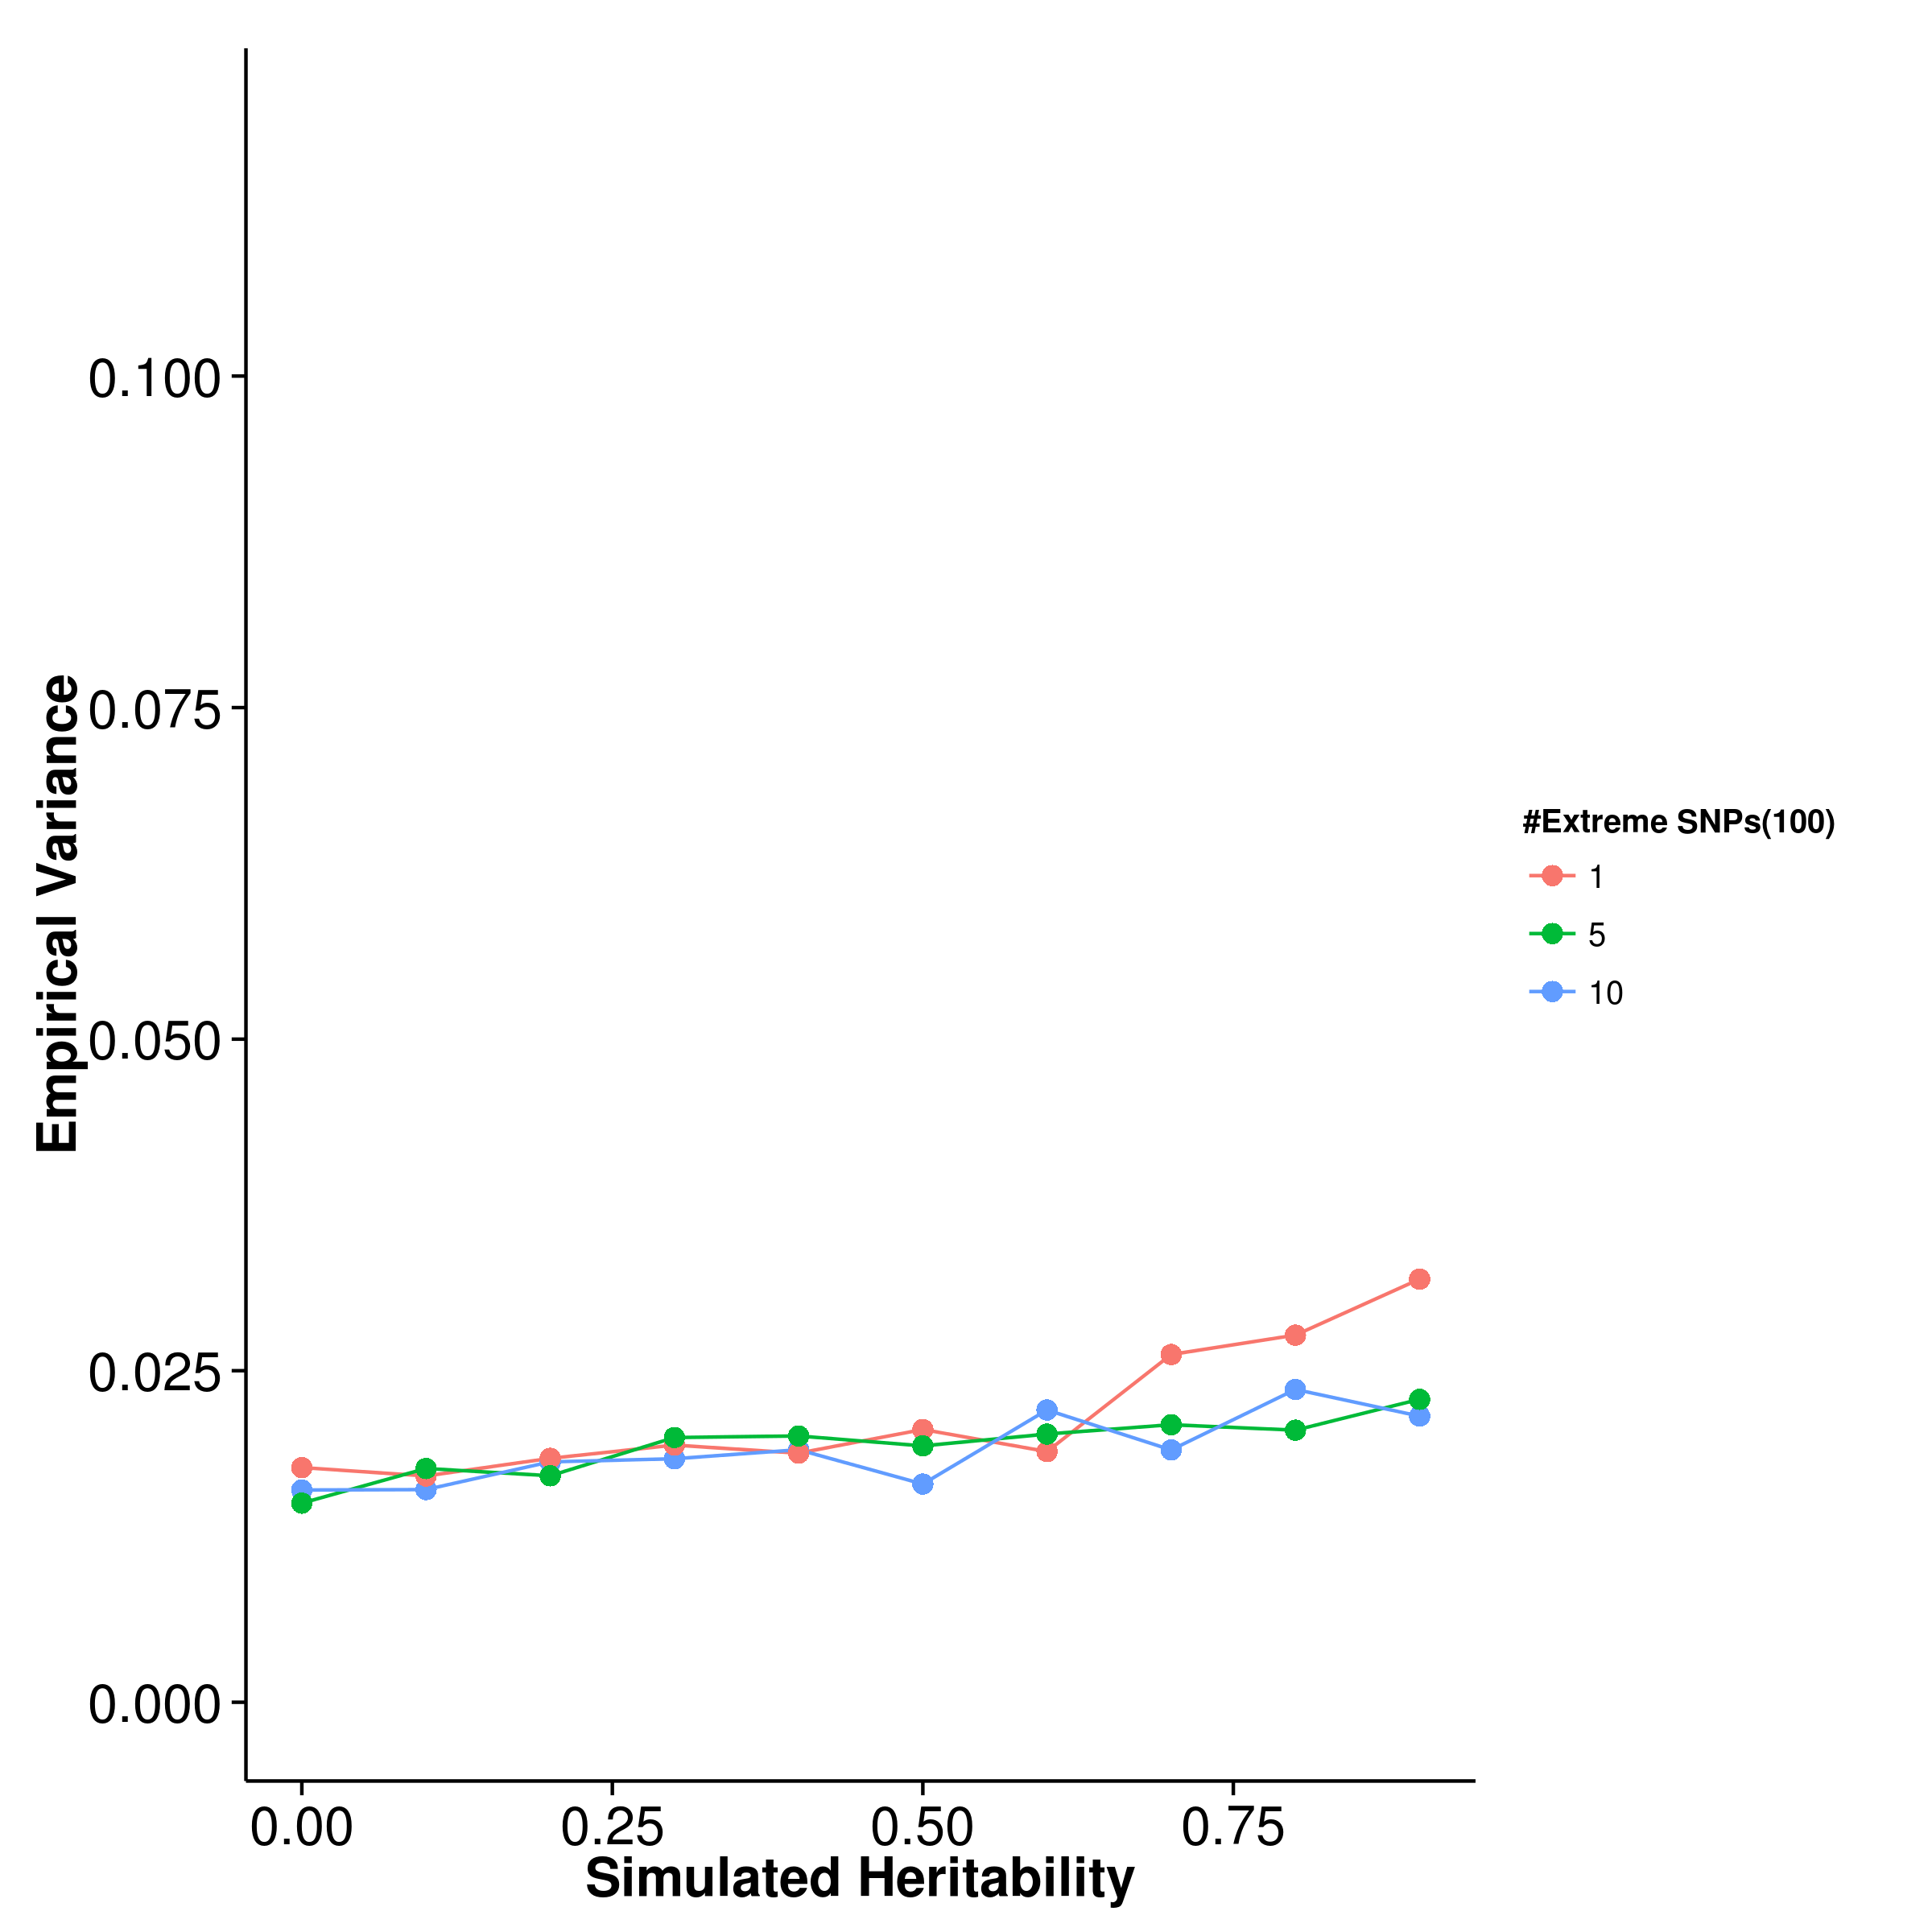
\includegraphics{figure/he_summary/extreme_100c/shrek_QtE_Rand_sd.png}}
				\label{fig:shrekQtEx100cVar}
			}
			\subfloat[GCTA]{
				\scalebox{.4}{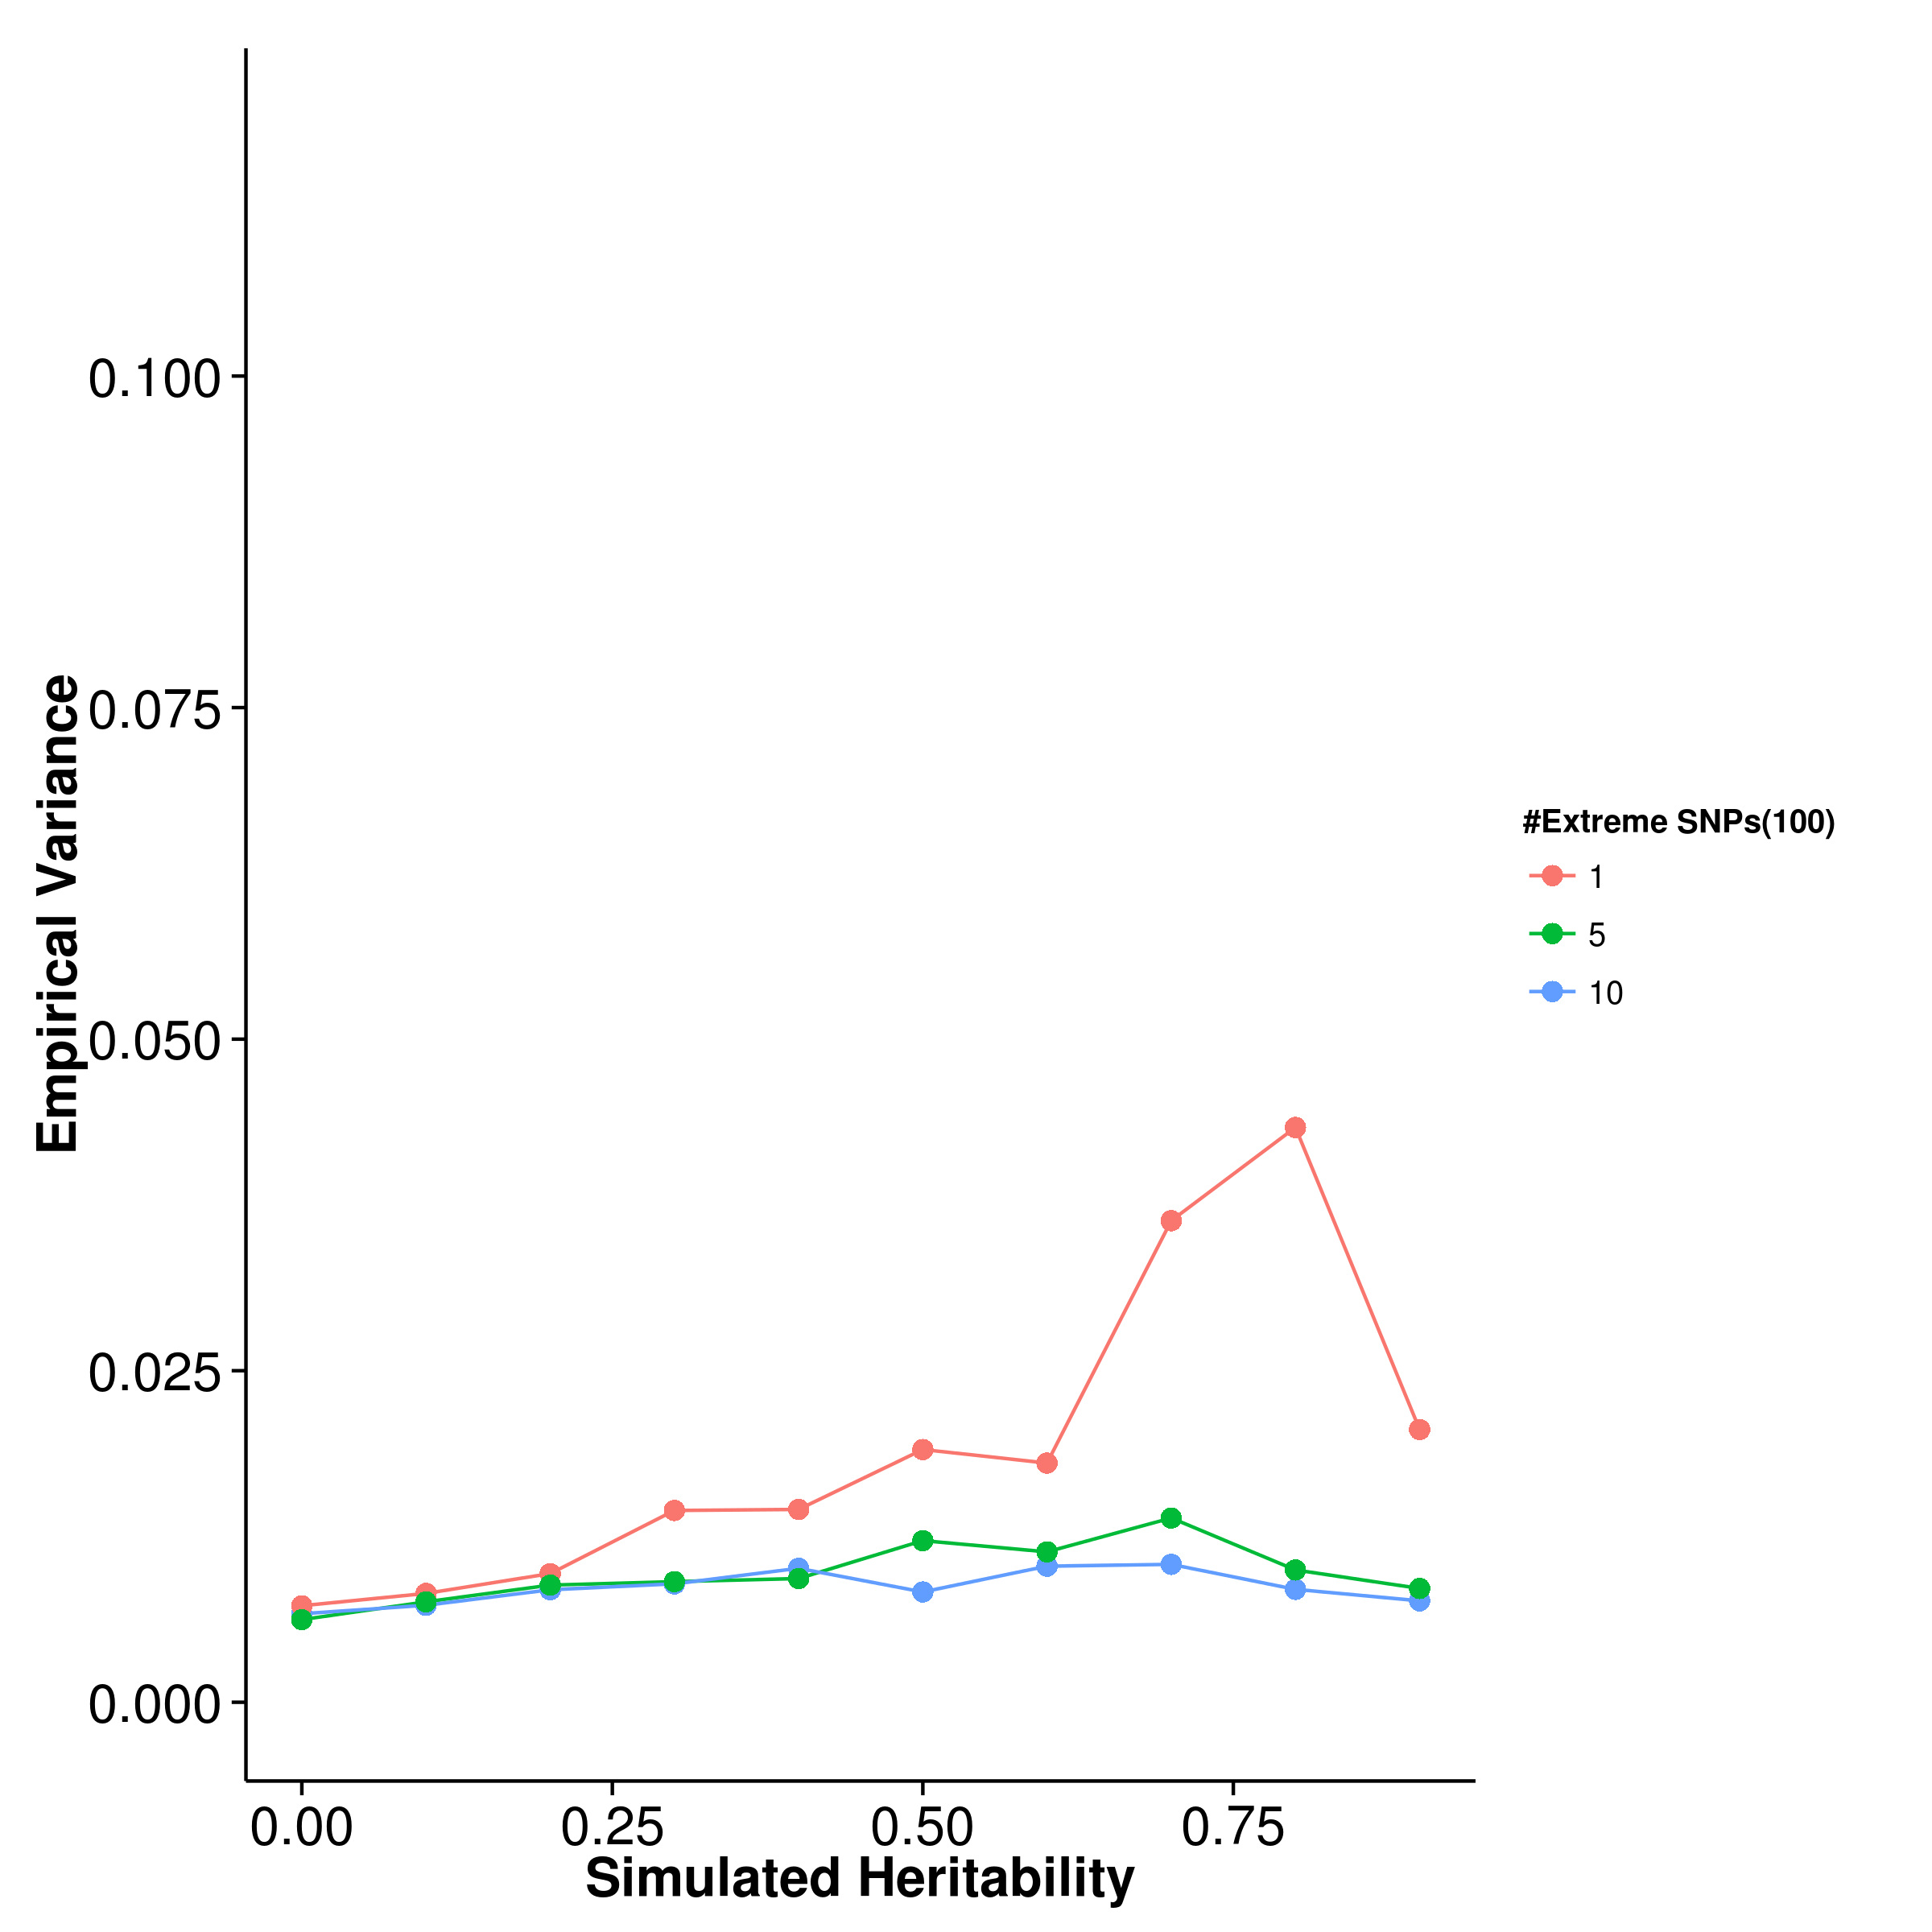
\includegraphics{figure/he_summary/extreme_100c/gcta_QtE_Rand_sd.png}}
				\label{fig:gctaQtEx100cVar}
			}\\
			\subfloat[LDSC with fix intercept]{
				\scalebox{.4}{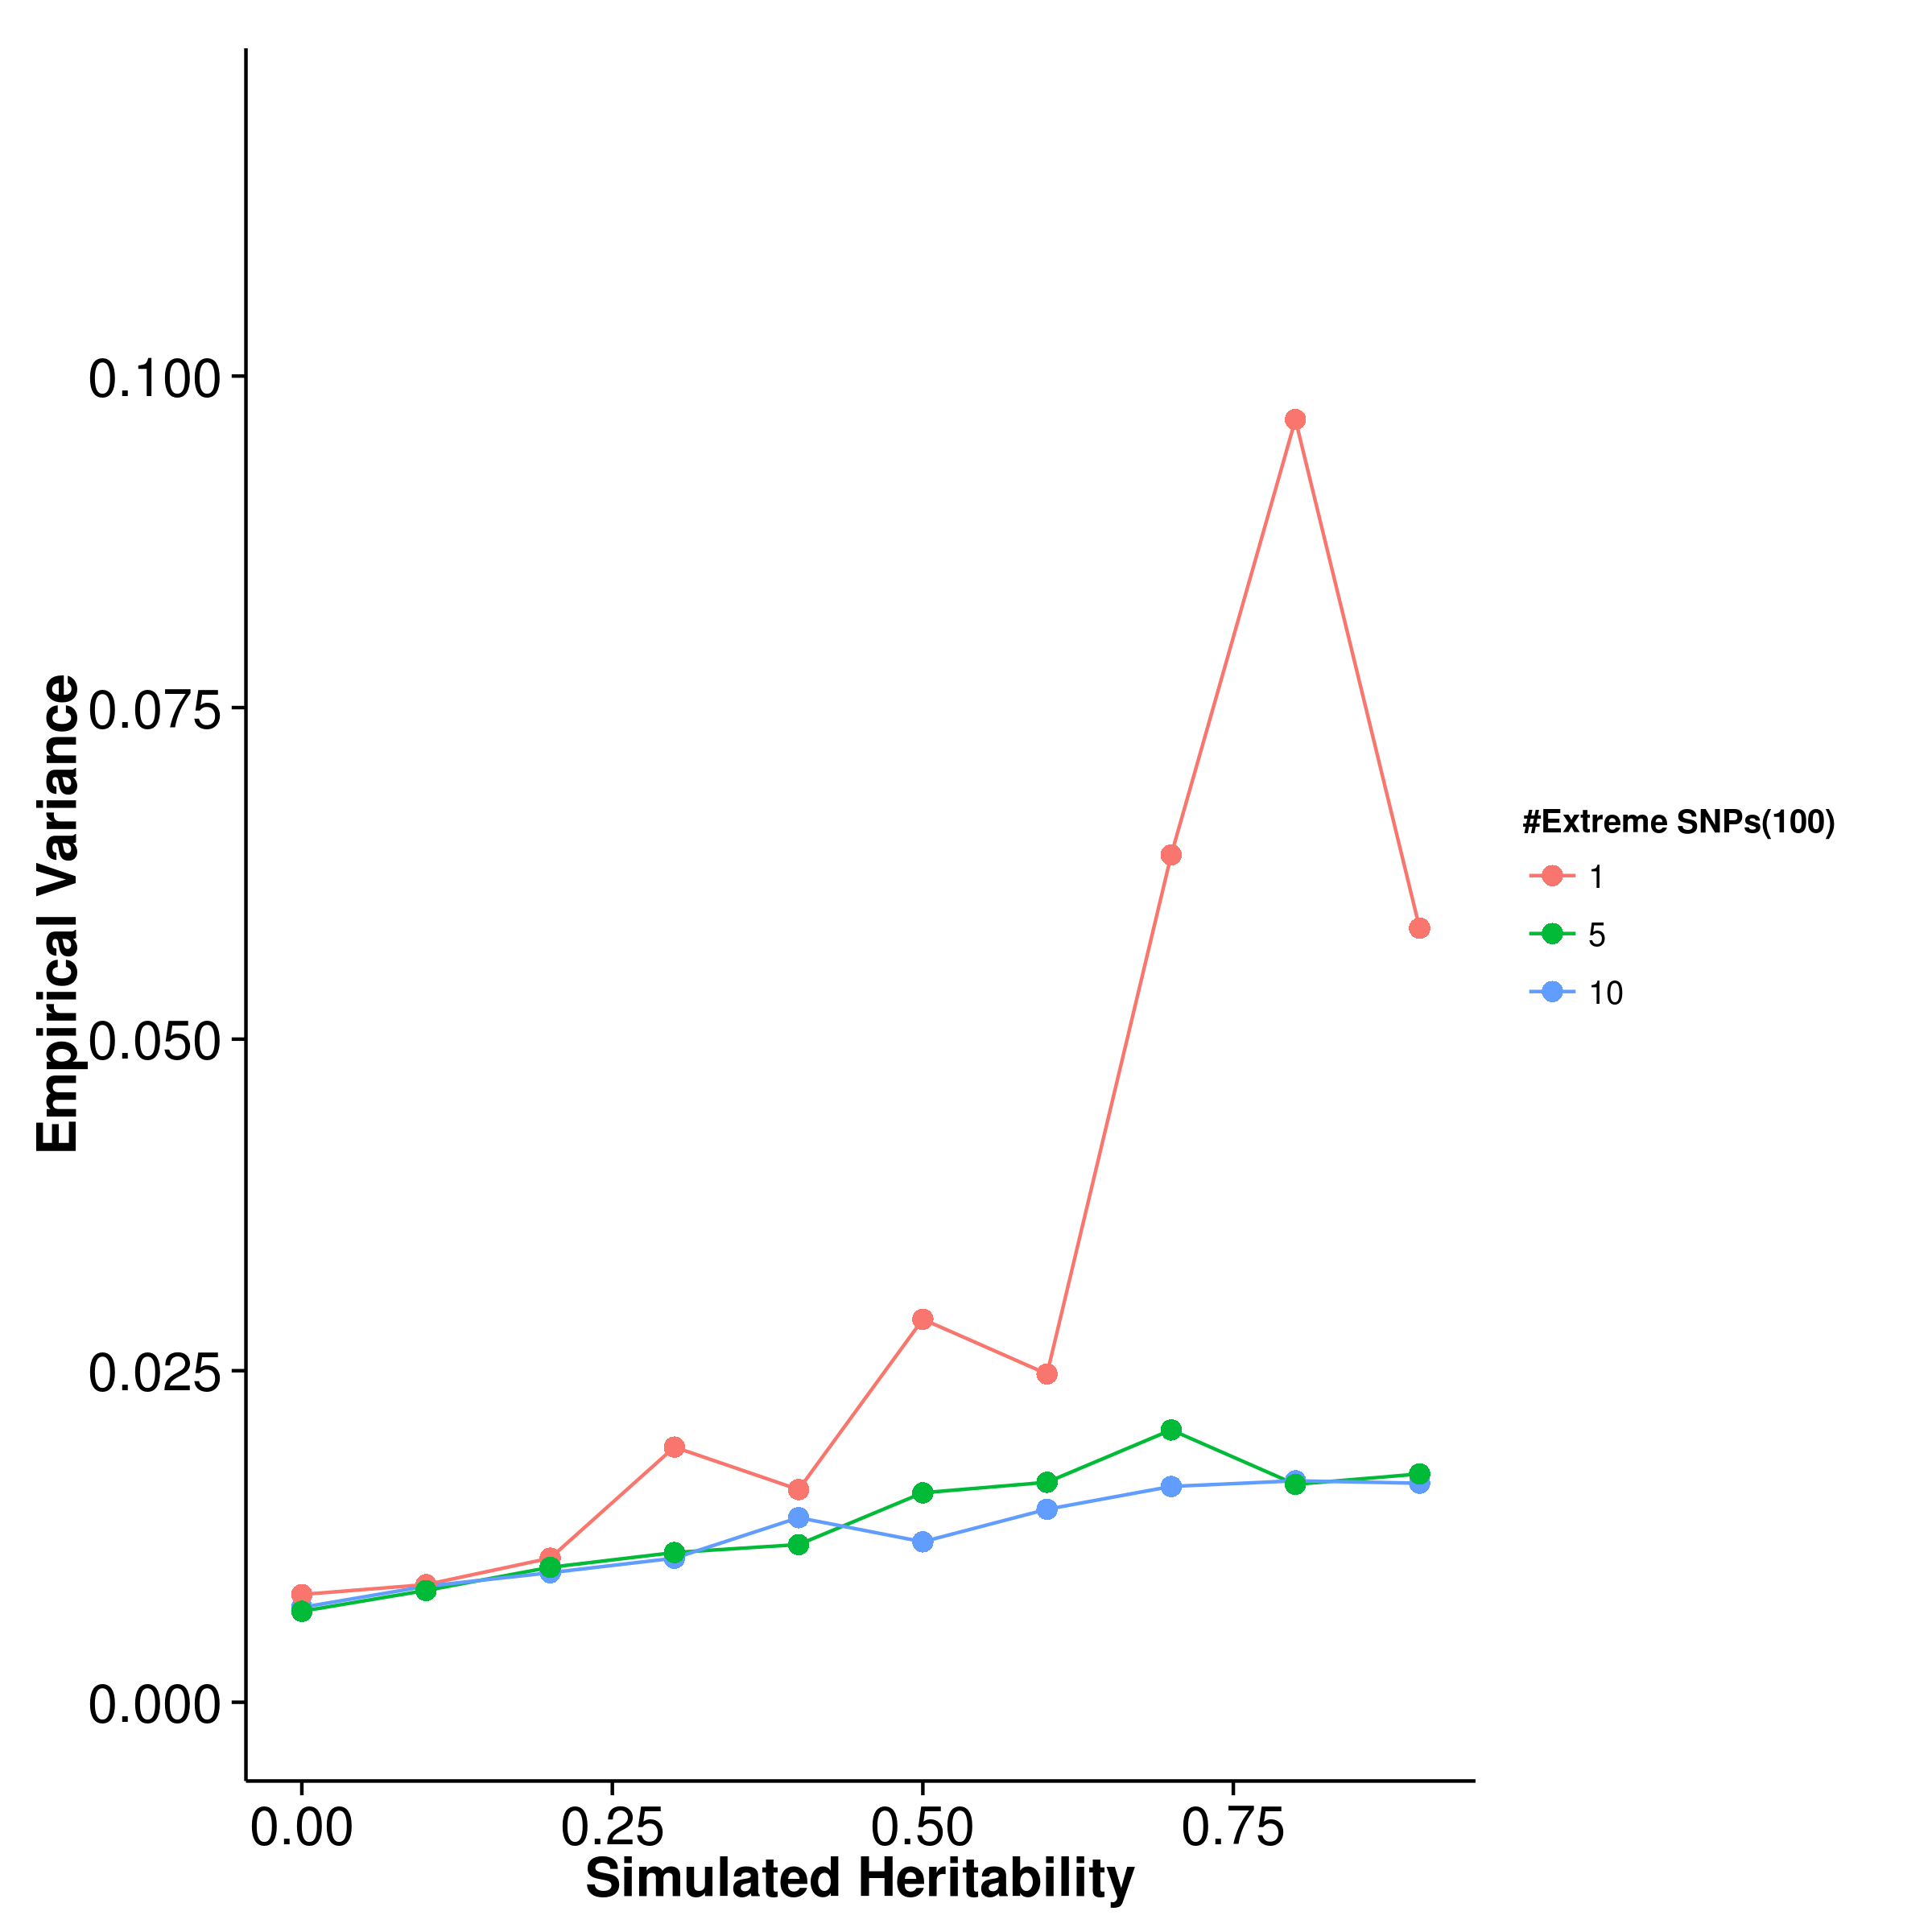
\includegraphics{figure/he_summary/extreme_100c/ldsc_QtE_Rand_sd.png}}
				\label{fig:ldscQtEx100cVar}
			}
			\subfloat[LDSC with intercept estimation]{
				
				\scalebox{.4}{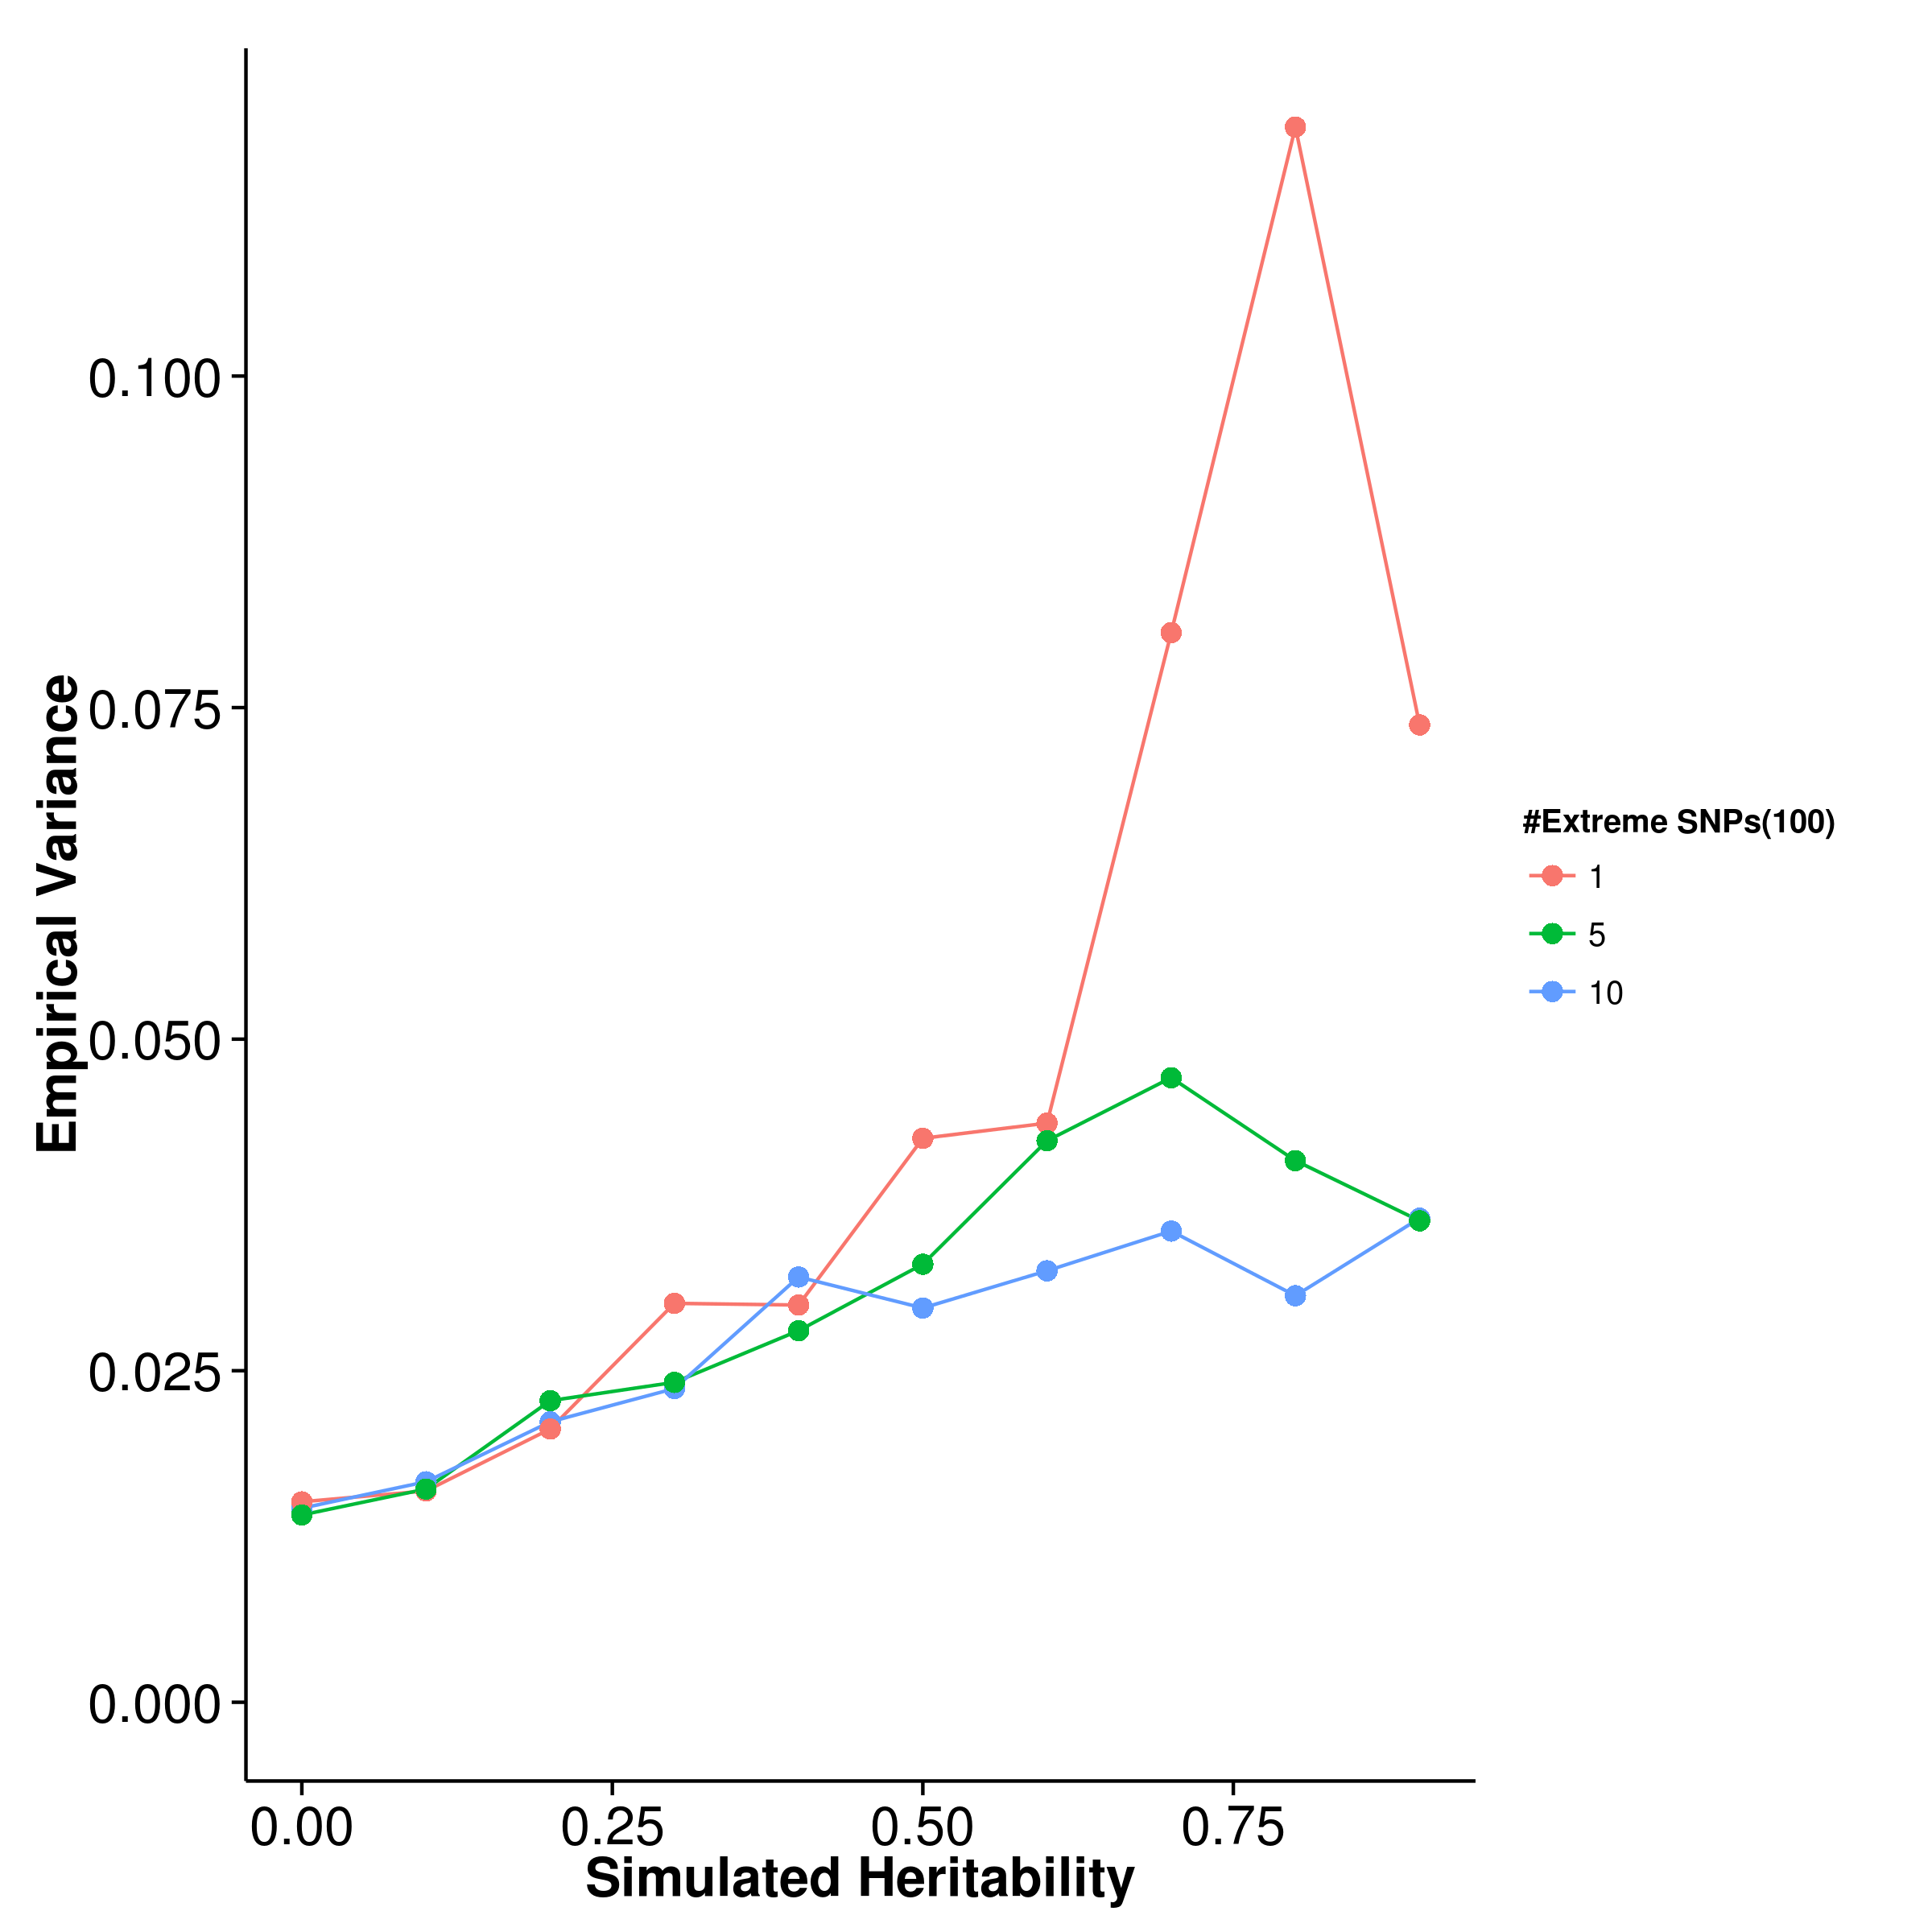
\includegraphics{figure/he_summary/extreme_100c/ldscIn_QtE_Rand_sd.png}}
				\label{fig:ldscInQtEx100cVar}
			}
			\caption[Variance of Extreme Effect Size Simulation Result]
			{Variance of results from quantitative trait simulation with extreme effect size simulation.
				100 causal \glspl{SNP} were simulated.
				When only 1 \gls{SNP} with extreme effect was simulated, the empirical variance of \gls{gcta} and \gls{ldsc} increases and a large fluctuation was observed.
				Whereas the empirical variance of \gls{shrek} only increases slightly when the simulated heritability is large and with only 1 \gls{SNP} with extreme effect.
				This suggests that \gls{shrek} is more robust to the change in number of extreme \gls{SNP}(s).
			} 
			\label{fig:QtEx100cVar}
		\end{figure}
		%Variance estimation
		\begin{figure}
			\centering
			\subfloat[SHREK]{
				\scalebox{.4}{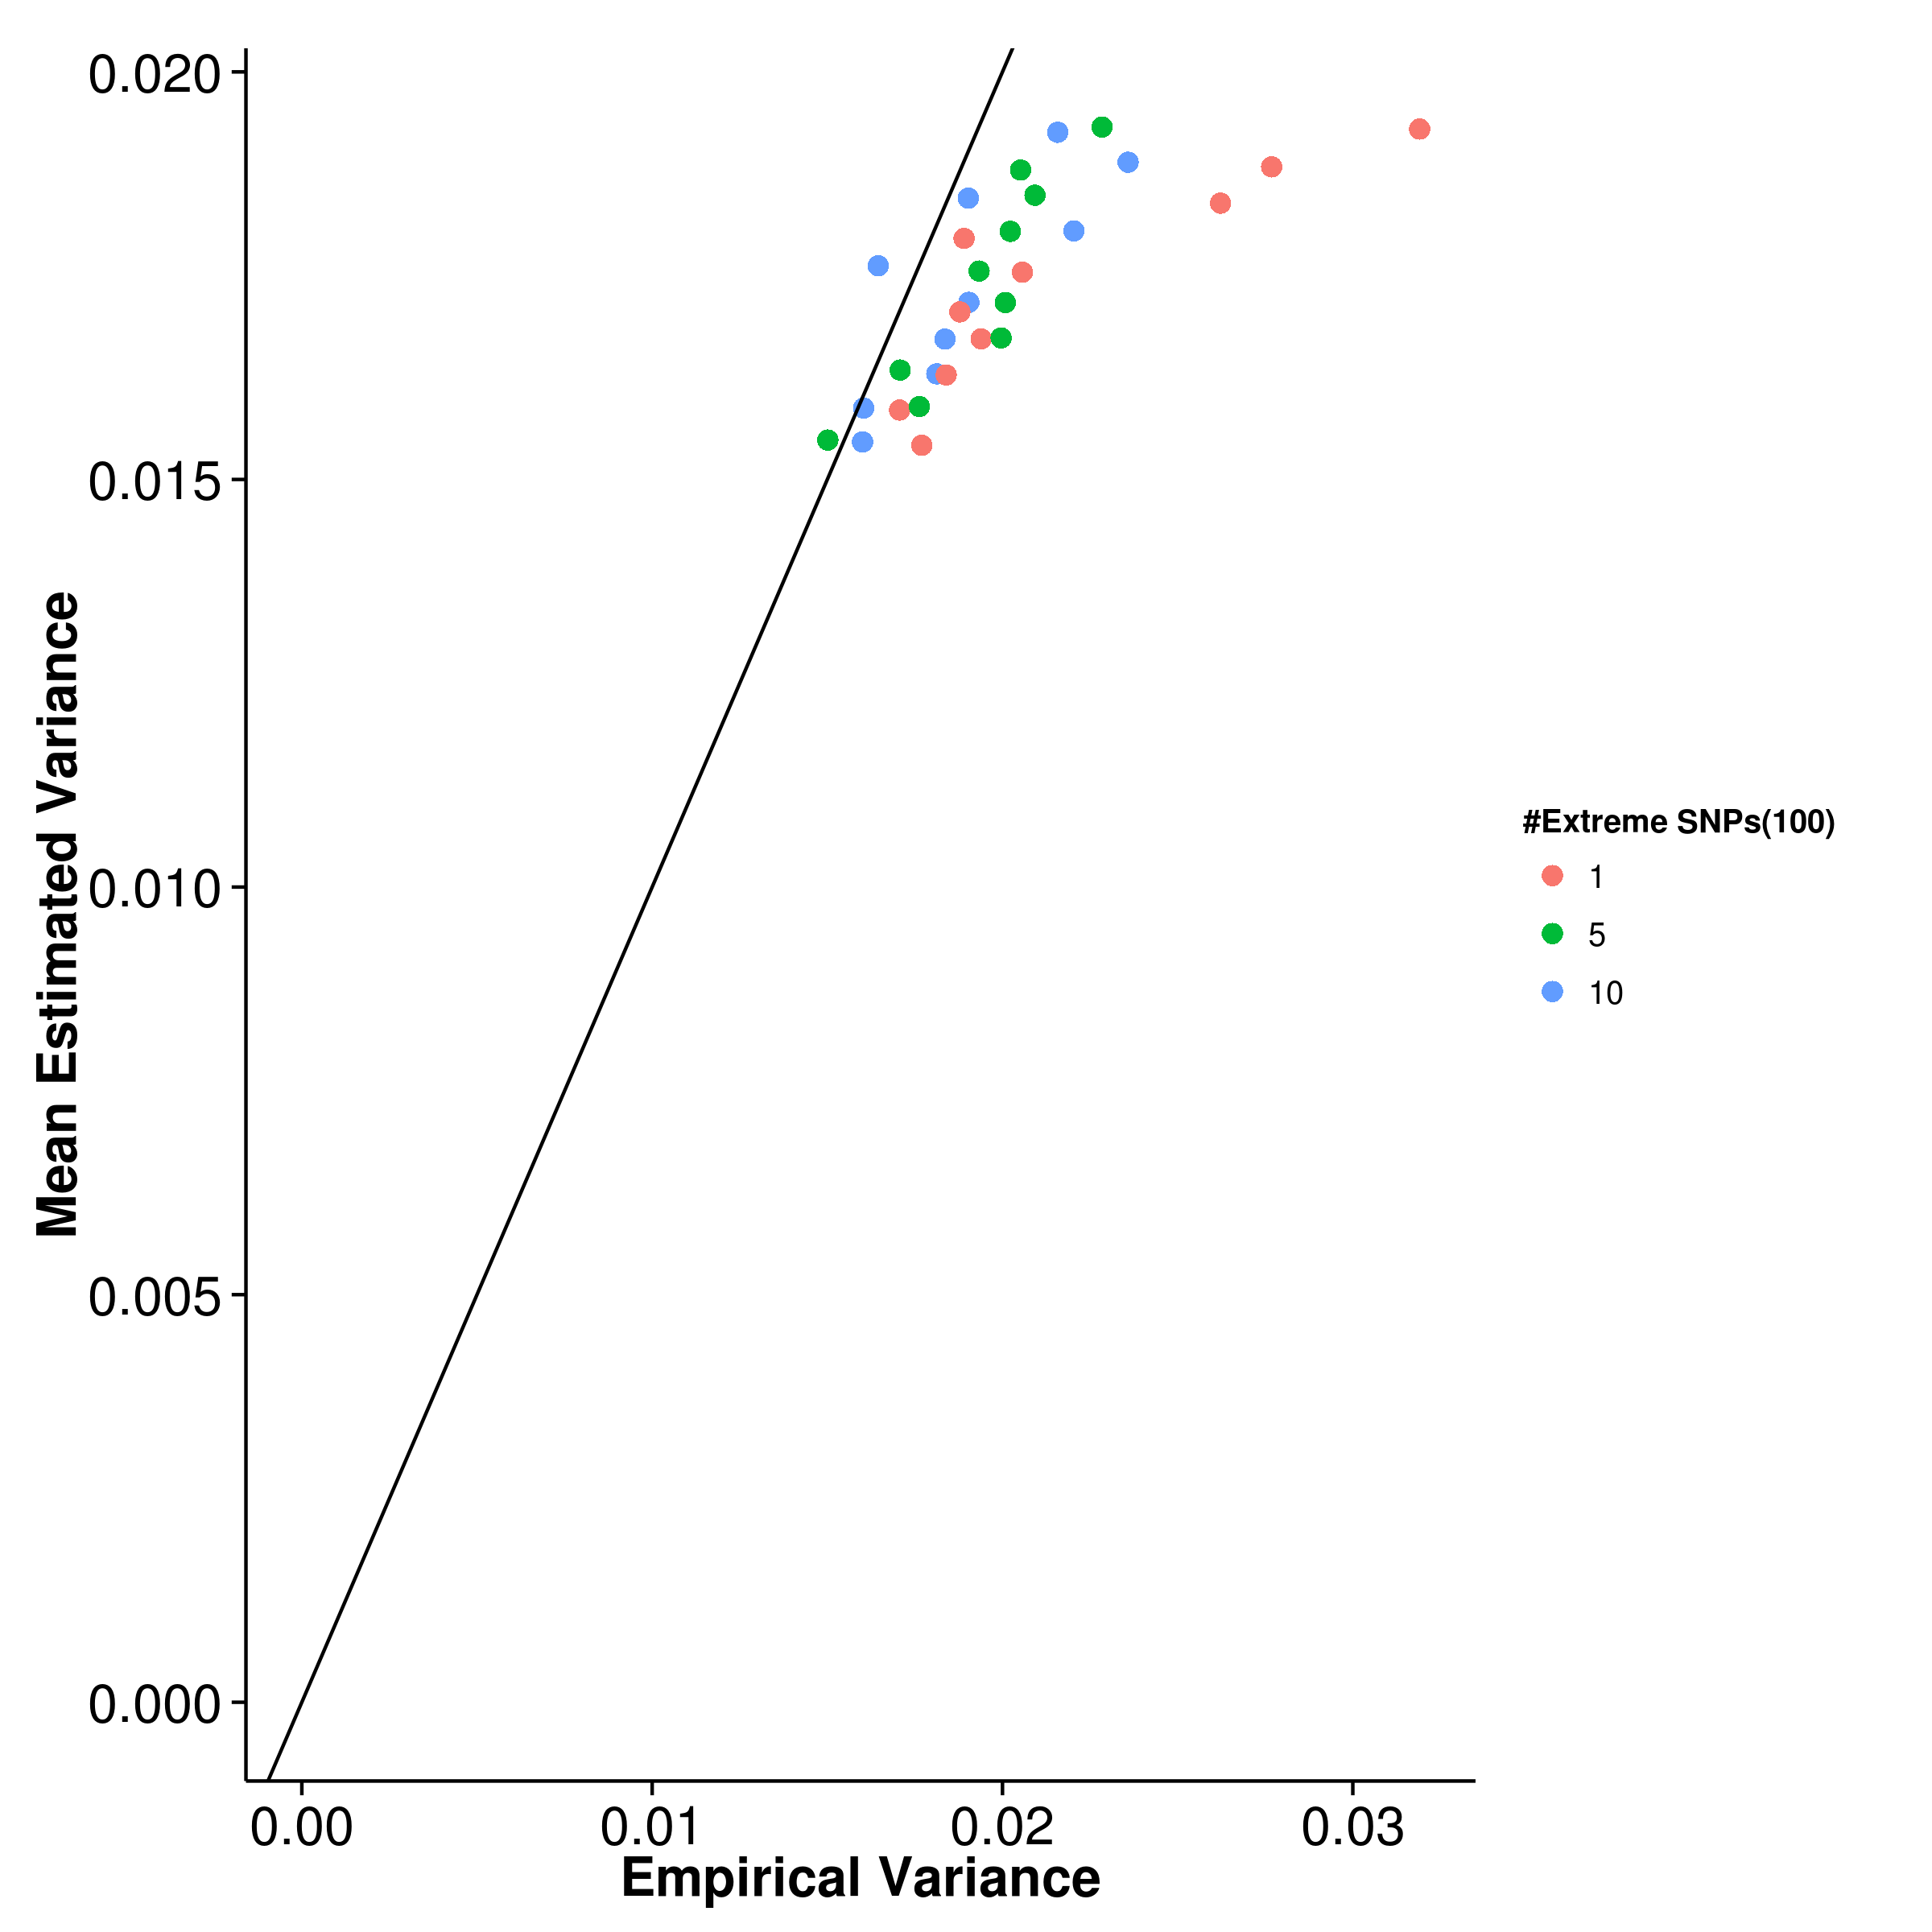
\includegraphics{figure/he_summary/extreme_100c/shrek_QtE_Rand_sdCom.png}}
				\label{fig:shrekQtEx100cVarCom}
			}
			\subfloat[GCTA]{
				\scalebox{.4}{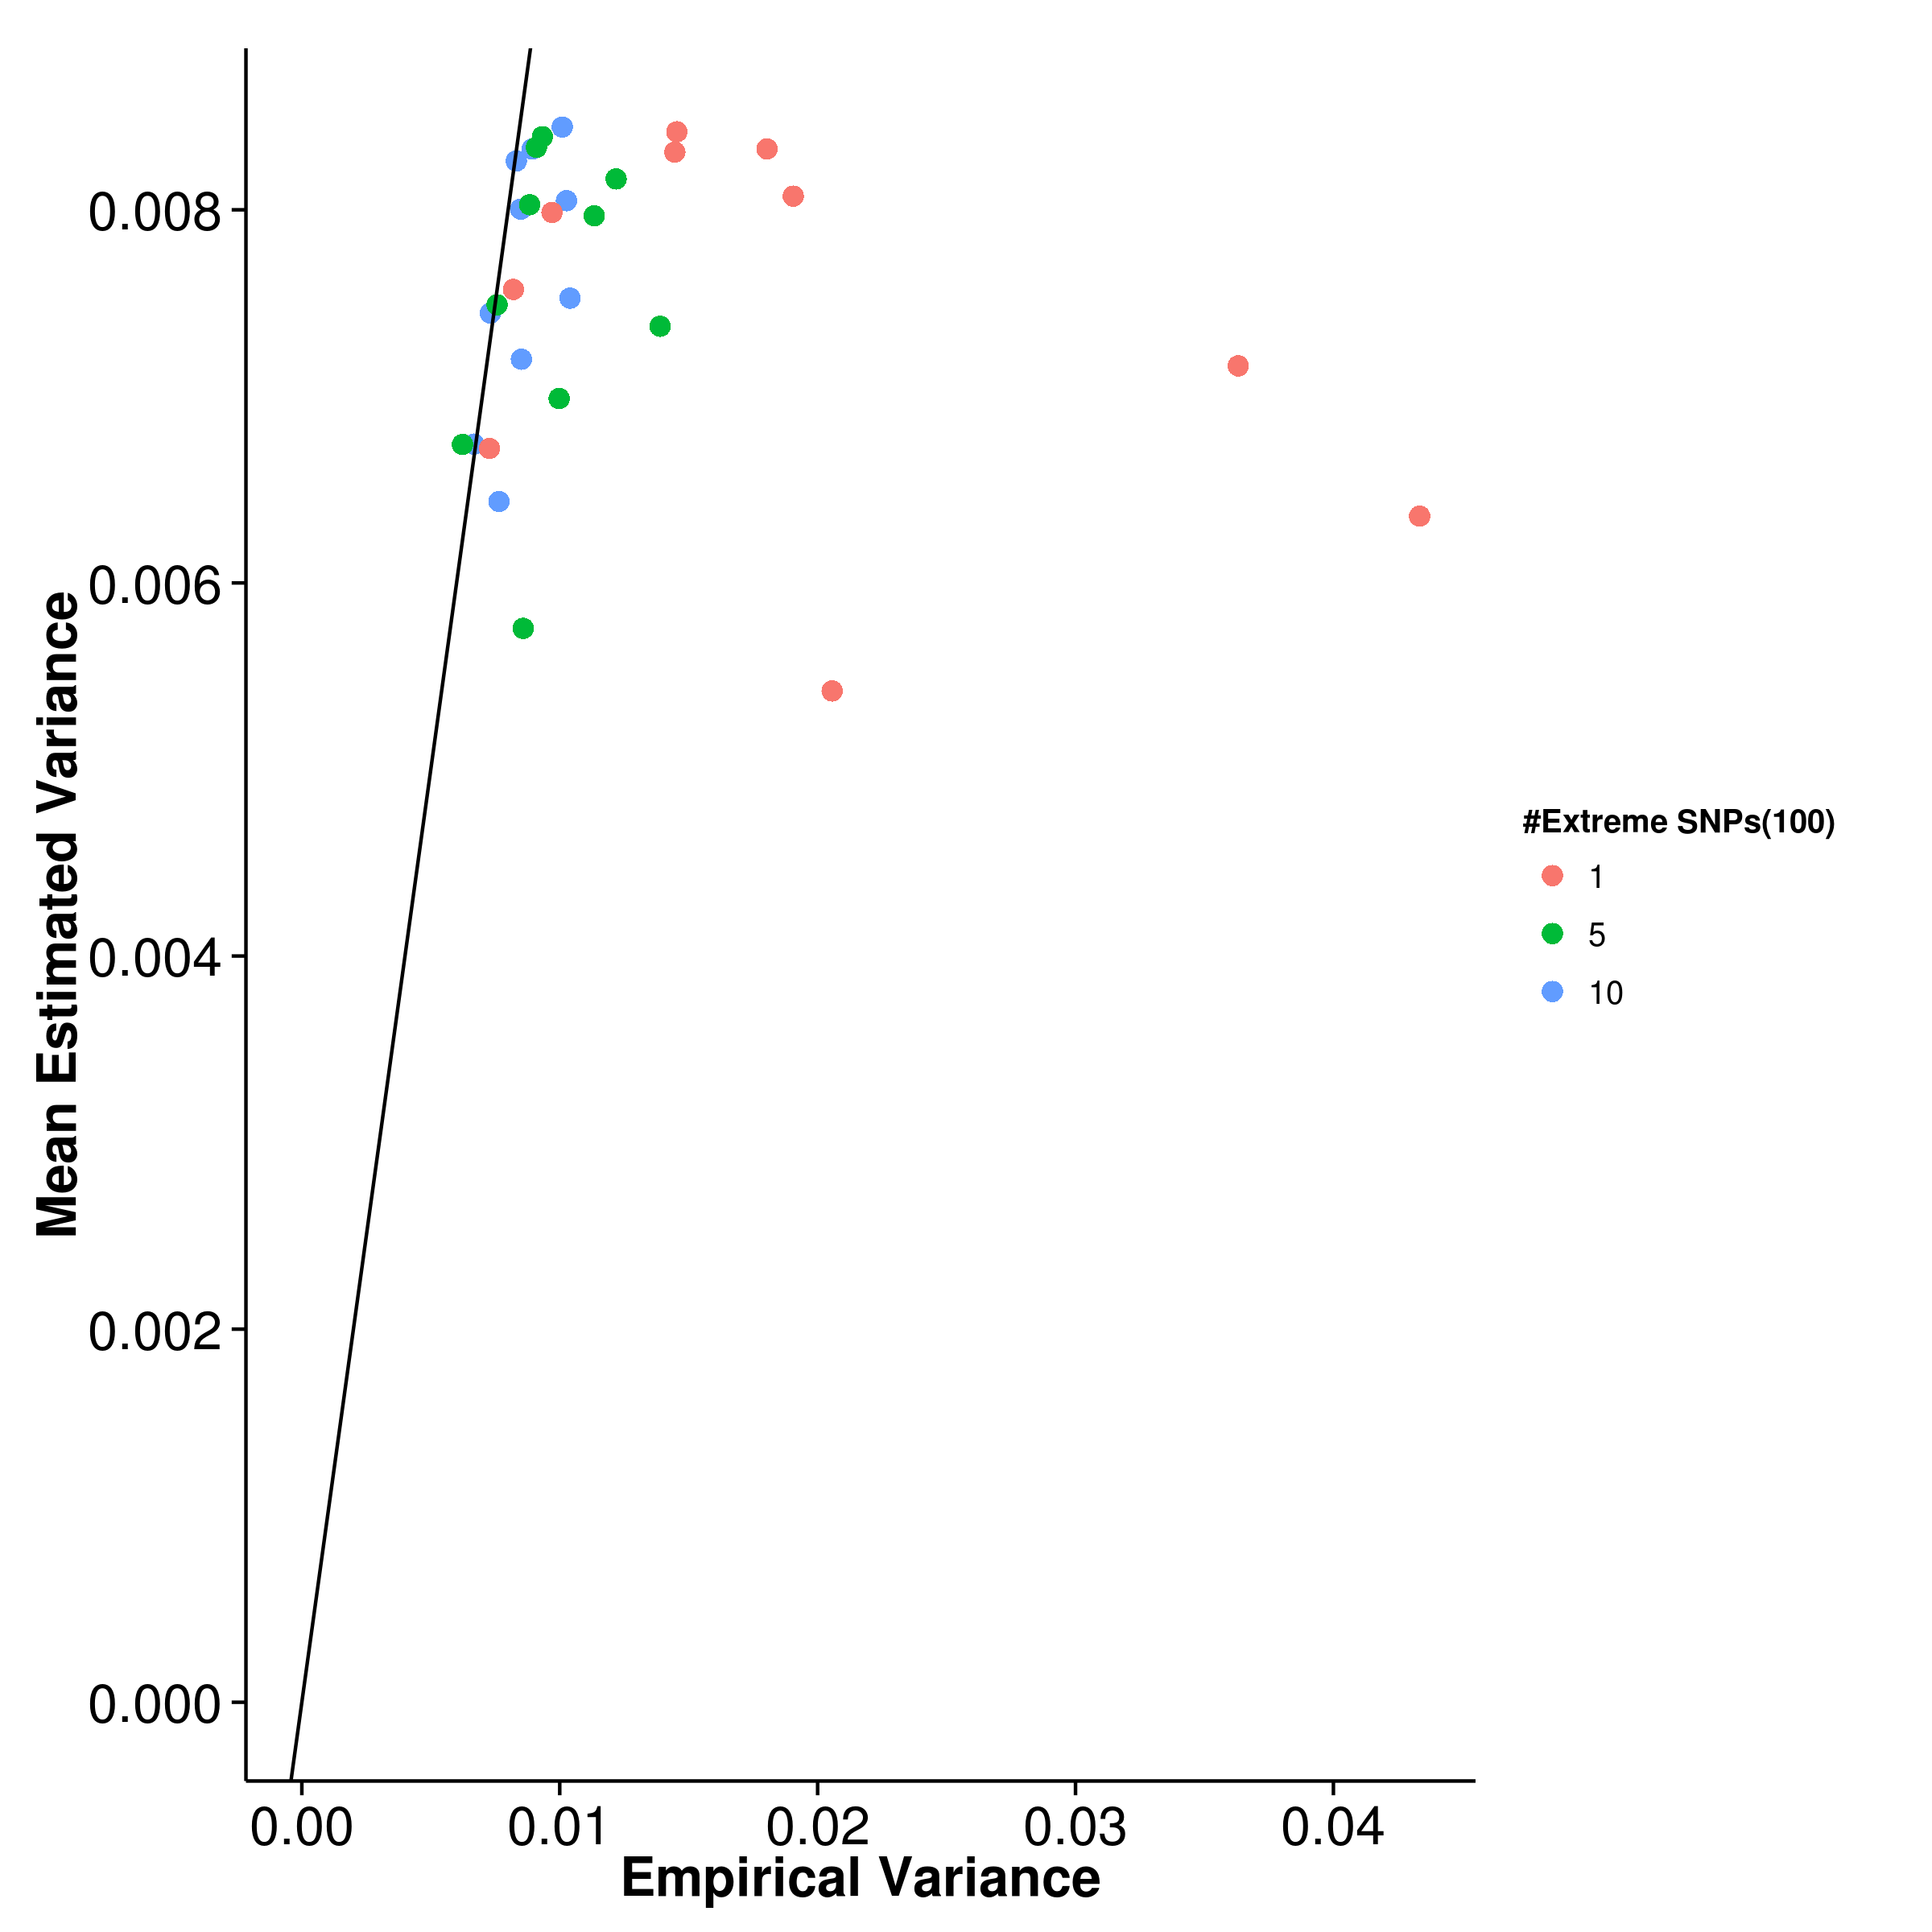
\includegraphics{figure/he_summary/extreme_100c/gcta_QtE_Rand_sdCom.png}}
				\label{fig:gctaQtEx100cVarCom}
			}\\
			\subfloat[LDSC with fix intercept]{
				\scalebox{.4}{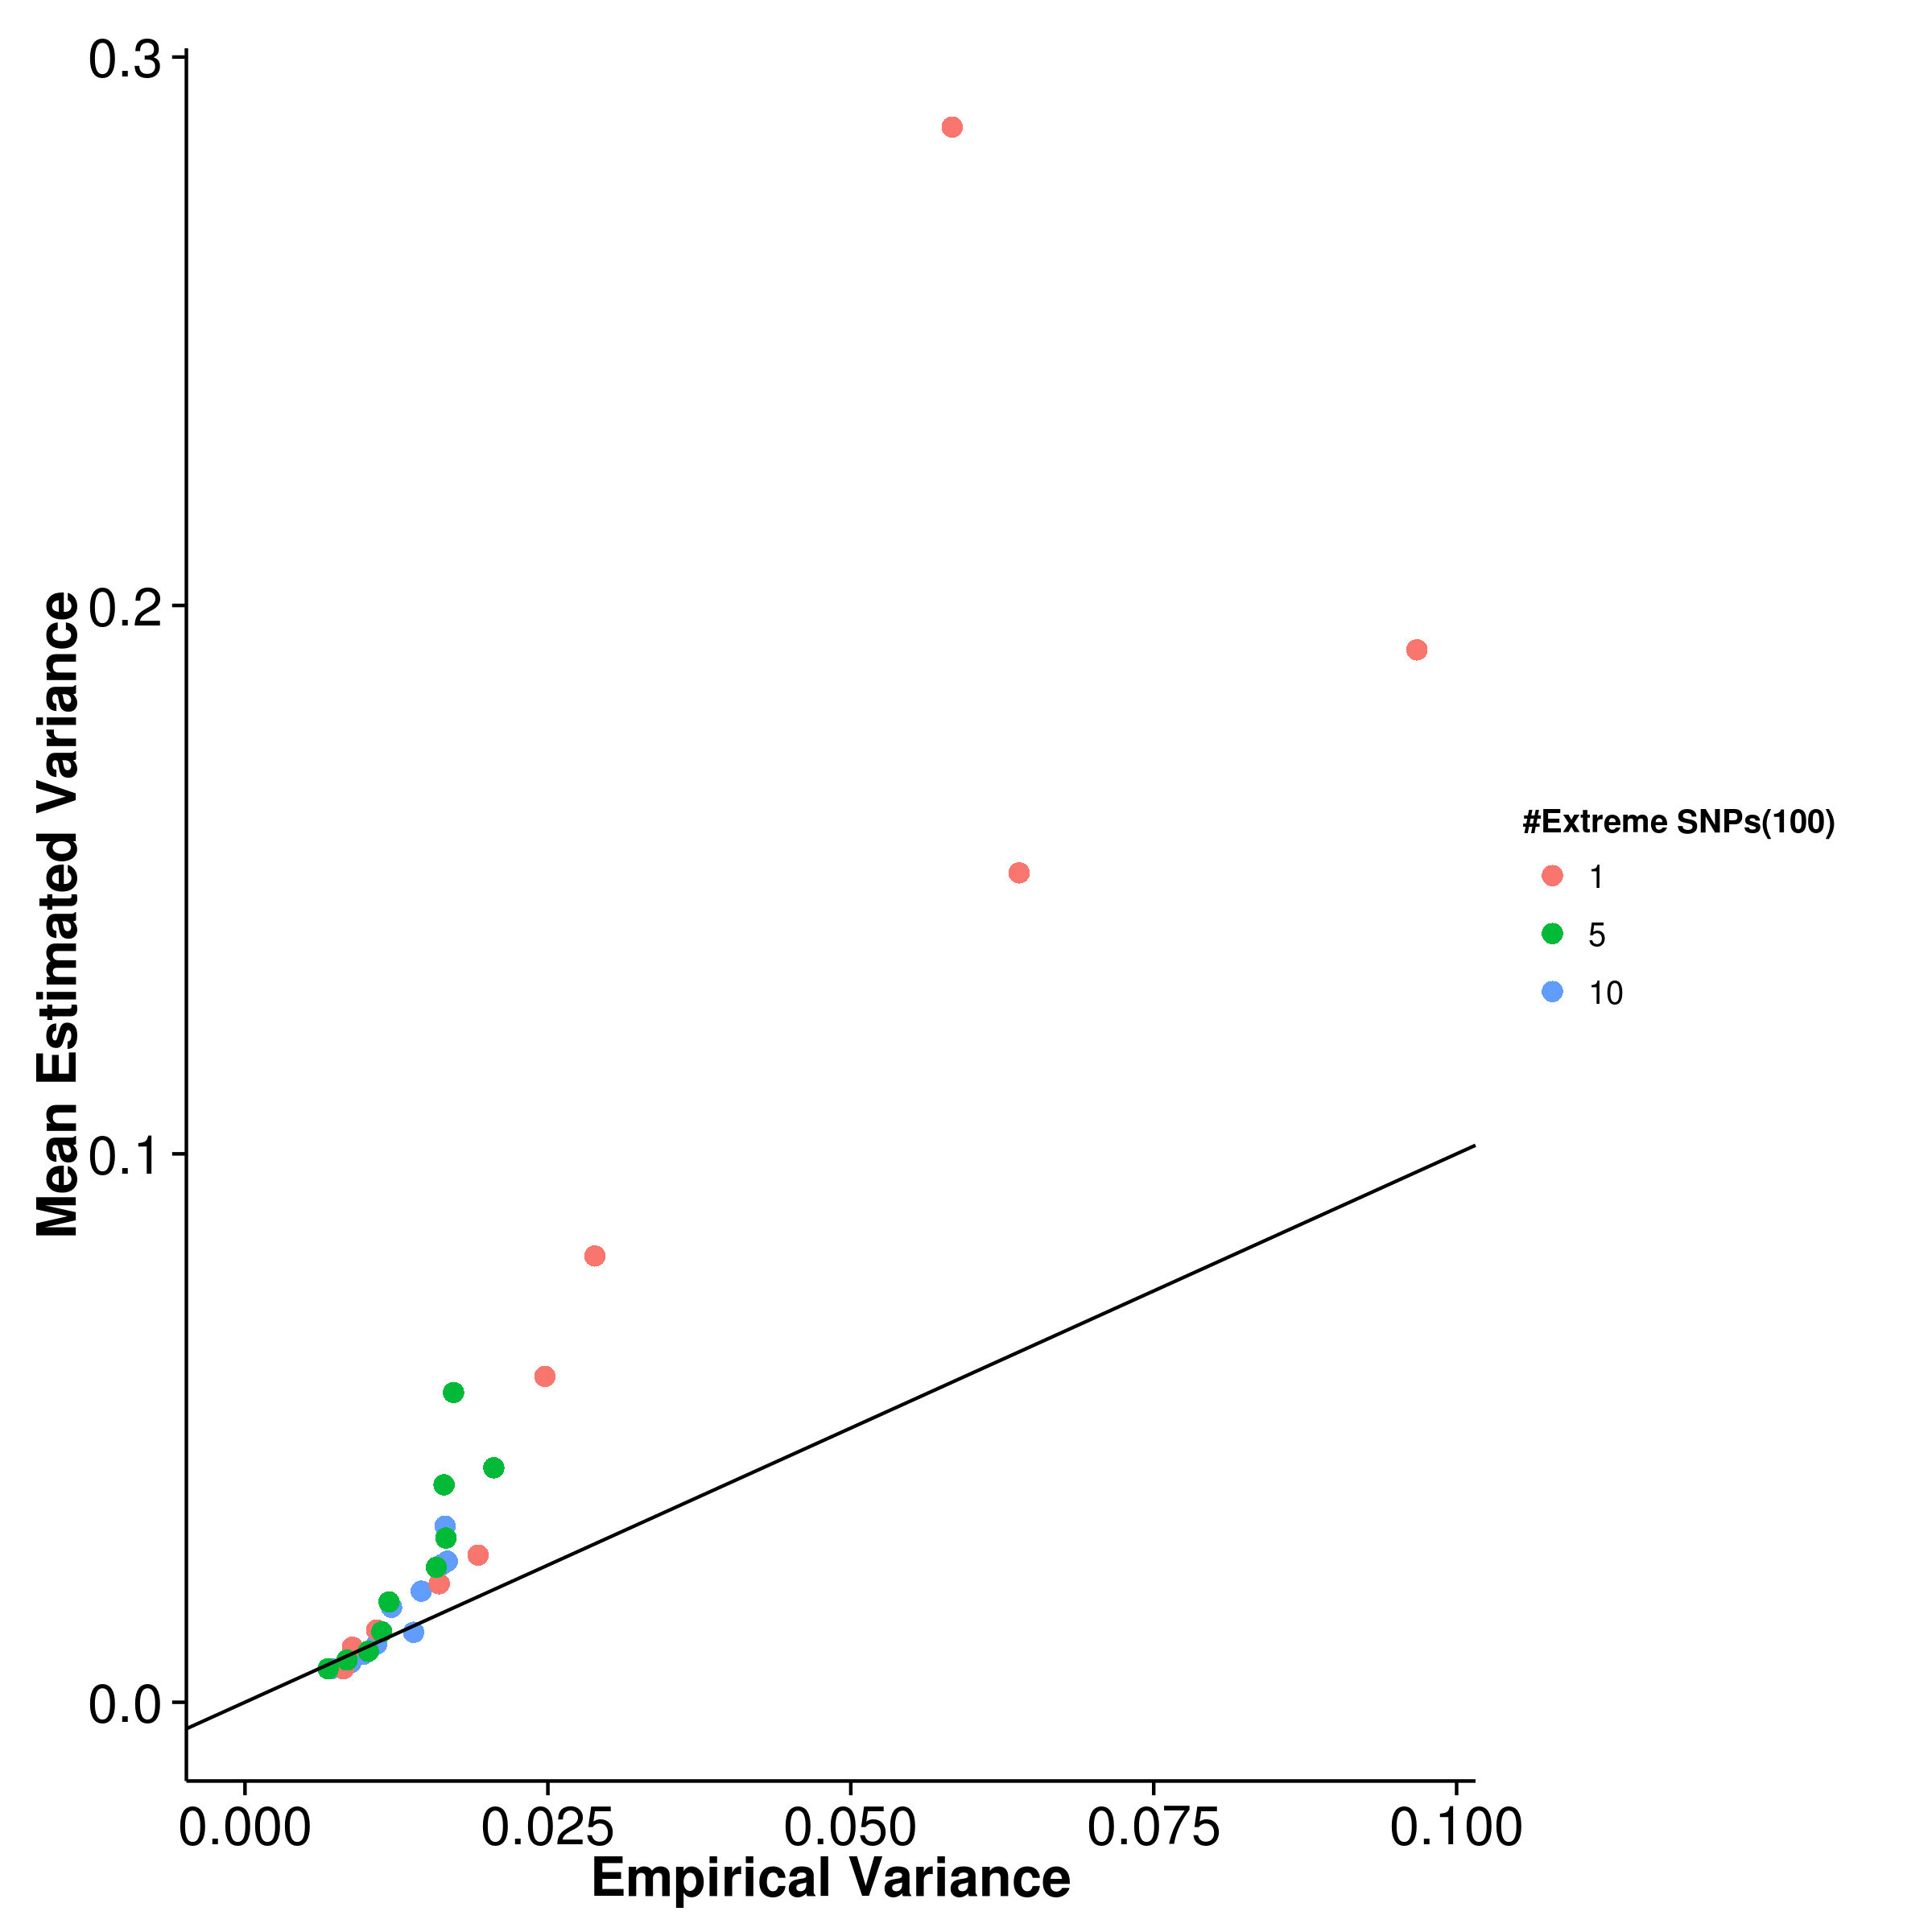
\includegraphics{figure/he_summary/extreme_100c/ldsc_QtE_Rand_sdCom.png}}
				\label{fig:ldscQtEx100cVarCom}
			}
			\subfloat[LDSC with intercept estimation]{
				
				\scalebox{.4}{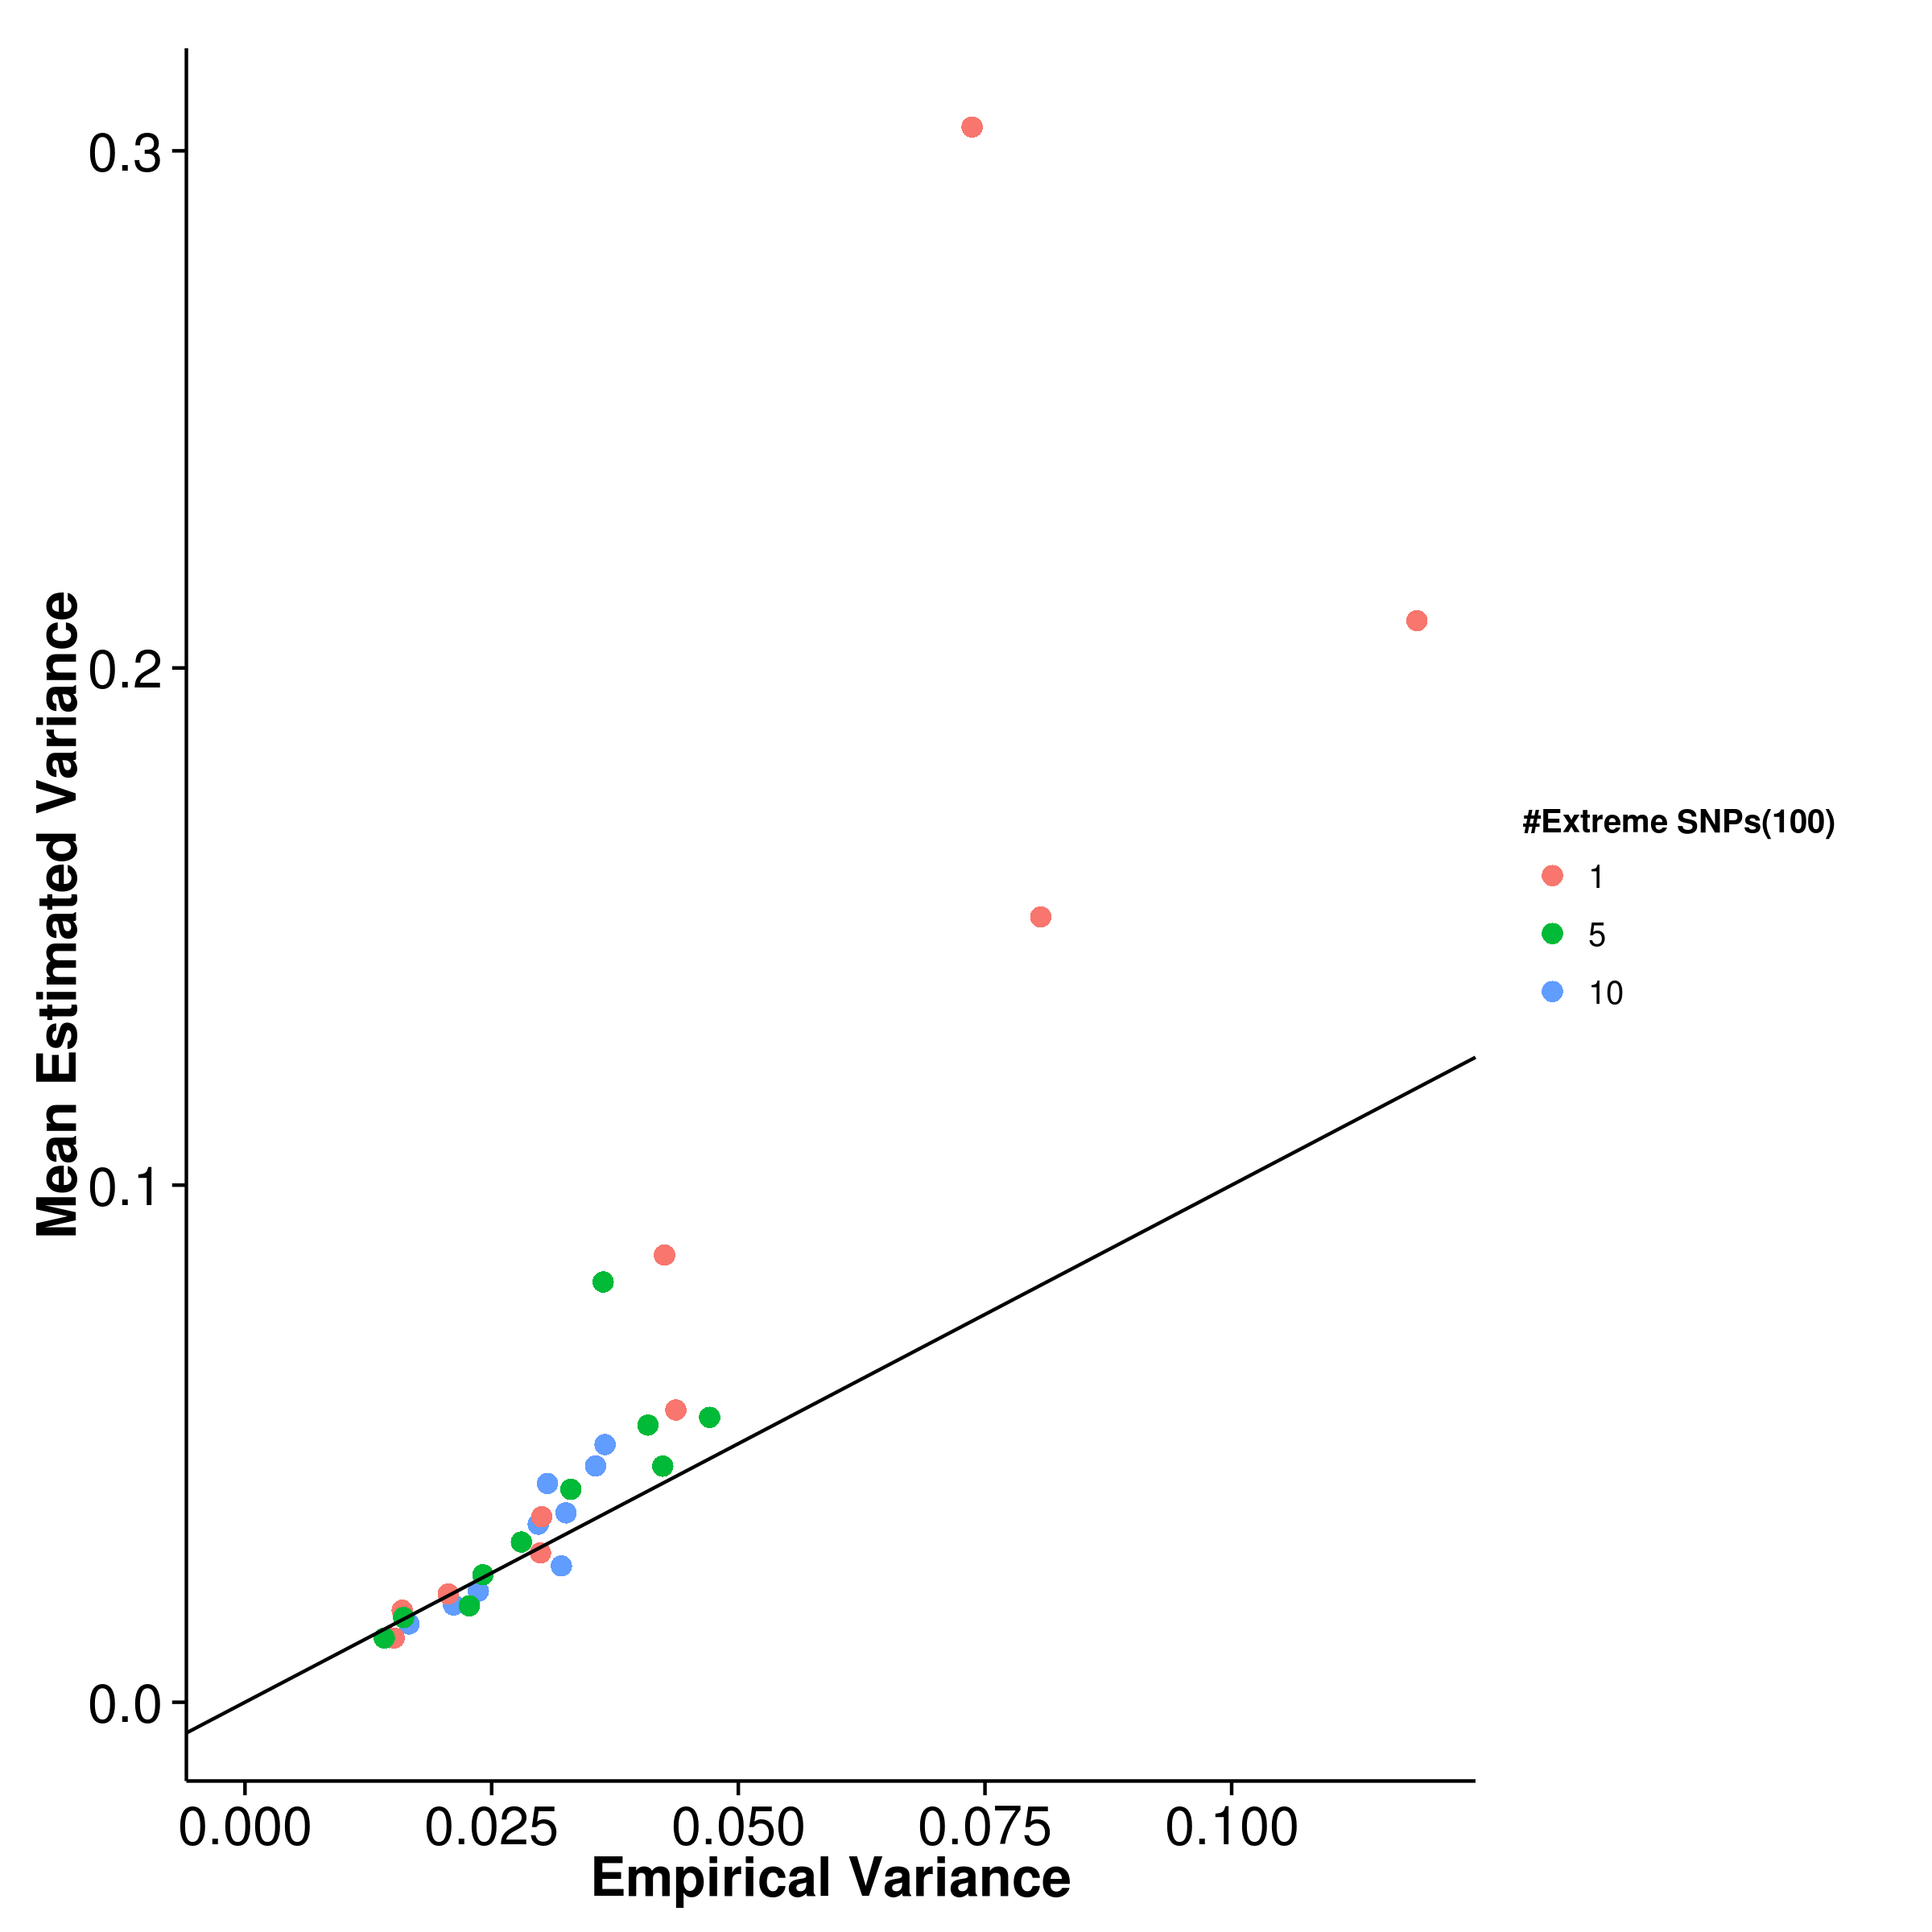
\includegraphics{figure/he_summary/extreme_100c/ldscIn_QtE_Rand_sdCom.png}}
				\label{fig:ldscInQtEx100cVarCom}
			}
			\caption[Estimation of Variance in Extreme Effect Size Simulation]
			{Estimated variance of results from quantitative trait simulation with extreme effect size simulation when compared to the empirical variance.
				100 causal \glspl{SNP} were simulated.
				\gls{shrek} and \gls{gcta} generally under-estimate the variance with the magnitude of bias being the highest when there is only 1 \gls{SNP} with extreme effect.
				On the other hand, \gls{ldsc} tends to over-estimate the variance and it can overestimate the variance by more than 3 folds when there is only 1 \gls{SNP} with extreme effect.
			} 
			\label{fig:QtEx100cVarCom}
		\end{figure}

		It is possible for a polygenic trait to have some portion of causal variants with much larger effect size when compared to other causal variants.
		In order to investigate how extreme effect size in a small number of causal \glspl{SNP} affect the \gls{SNP} heritability estimation, simulations were performed with trait that has 100 causal \glspl{SNP} where 1,5 or 10 of those \gls{SNP}(s) has a large effect.
		
		The overall performance of the algorithms are similar to the results observed in the quantitative trait simulation (\cref{fig:QtEx100cMean}).
		However, when 1 of the causal \glspl{SNP} was simulated with large effect, the mean estimates from \gls{ldsc} and \gls{gcta} fluctuate (\cref{fig:gctaQtEx100cMean,fig:ldscQtEx100cMean,fig:ldscInQtEx100cMean}).
		The same fluctuation is not observed in \gls{shrek} (\cref{fig:shrekQtEx100cMean}). 
		Similarly, the empirical variance of the estimates (\cref{fig:QtEx100cVar}) from \gls{gcta} and \gls{ldsc} increase and fluctuate when only 1 of the causal \glspl{SNP} was simulated with large effect.
		Again, the estimates from \gls{shrek} are robust to change in number of \gls{SNP} with large effect size.
		
		When inspecting the variance estimation, it is observed that both \gls{shrek} and \gls{gcta} underestimate their empirical variance. 
		As the number of \gls{SNP}(s) with large effect size decreases, the magnitude of bias increases.
		On the other hand, it is observed that \gls{ldsc} tends to overestimate its empirical variance. 
		When the intercept is fixed, the estimated variance from \gls{ldsc} can be as much as 3 fold larger than the empirical variance when only 1 of the causal \gls{SNP} with large effect size was simulated. 
		
		To conclude, \gls{gcta} has the best performance among the algorithms tested (\cref{tab:mseEx100c}).
		However, for studies which only summary statistics are available, \gls{gcta} analysis cannot be performed. 
		In such scenario, \gls{shrek} has a better performance when compared to \gls{ldsc} when only 1 of the causal \glspl{SNP} carries a large effect size.
		Moreover, it is also observed that \gls{shrek} is more robust to change in number of \glspl {SNP} with large effect size. 
		
		\begin{table}
			\centering
			\begin{tabular}{rrrrr}
				\toprule
				Number of Extreme SNPs&	SHREK&	LDSC&	LDSC-In&	GCTA \\
				\midrule
				1	&	0.0227	&	0.0393	&	0.0508	&	0.0206\\
				5	&	0.0203	&	0.0145	&	0.0316	&	0.00985\\
				10	&	0.0205	&	0.0129	&	0.0329	&	0.00939\\
				\bottomrule
			\end{tabular}
			\caption[MSE of Quantitative Trait Simulation with Extreme Effect Size]{
				\gls{mse} of quantitative trait simulation with extreme effect size.
				Of all the algorithms, \gls{gcta} has the lowest \gls{mse}.
				When comparing the performance of \gls{shrek} and \gls{ldsc}, it is observed that \gls{ldsc} performs better unless only 1 of the causal \gls{SNP} has a large effect size.
				However, it is also observed that the performance of \gls{shrek} is robust to the change in number of \glspl{SNP} with extreme effect size.
				}
			\label{tab:mseEx100c}
		\end{table}
		
		% CC Rand Effect
		\subsubsection{Case Control Simulation}
			%Mean
			\begin{figure}
				\centering
				\subfloat[SHREK]{
					\scalebox{.4}{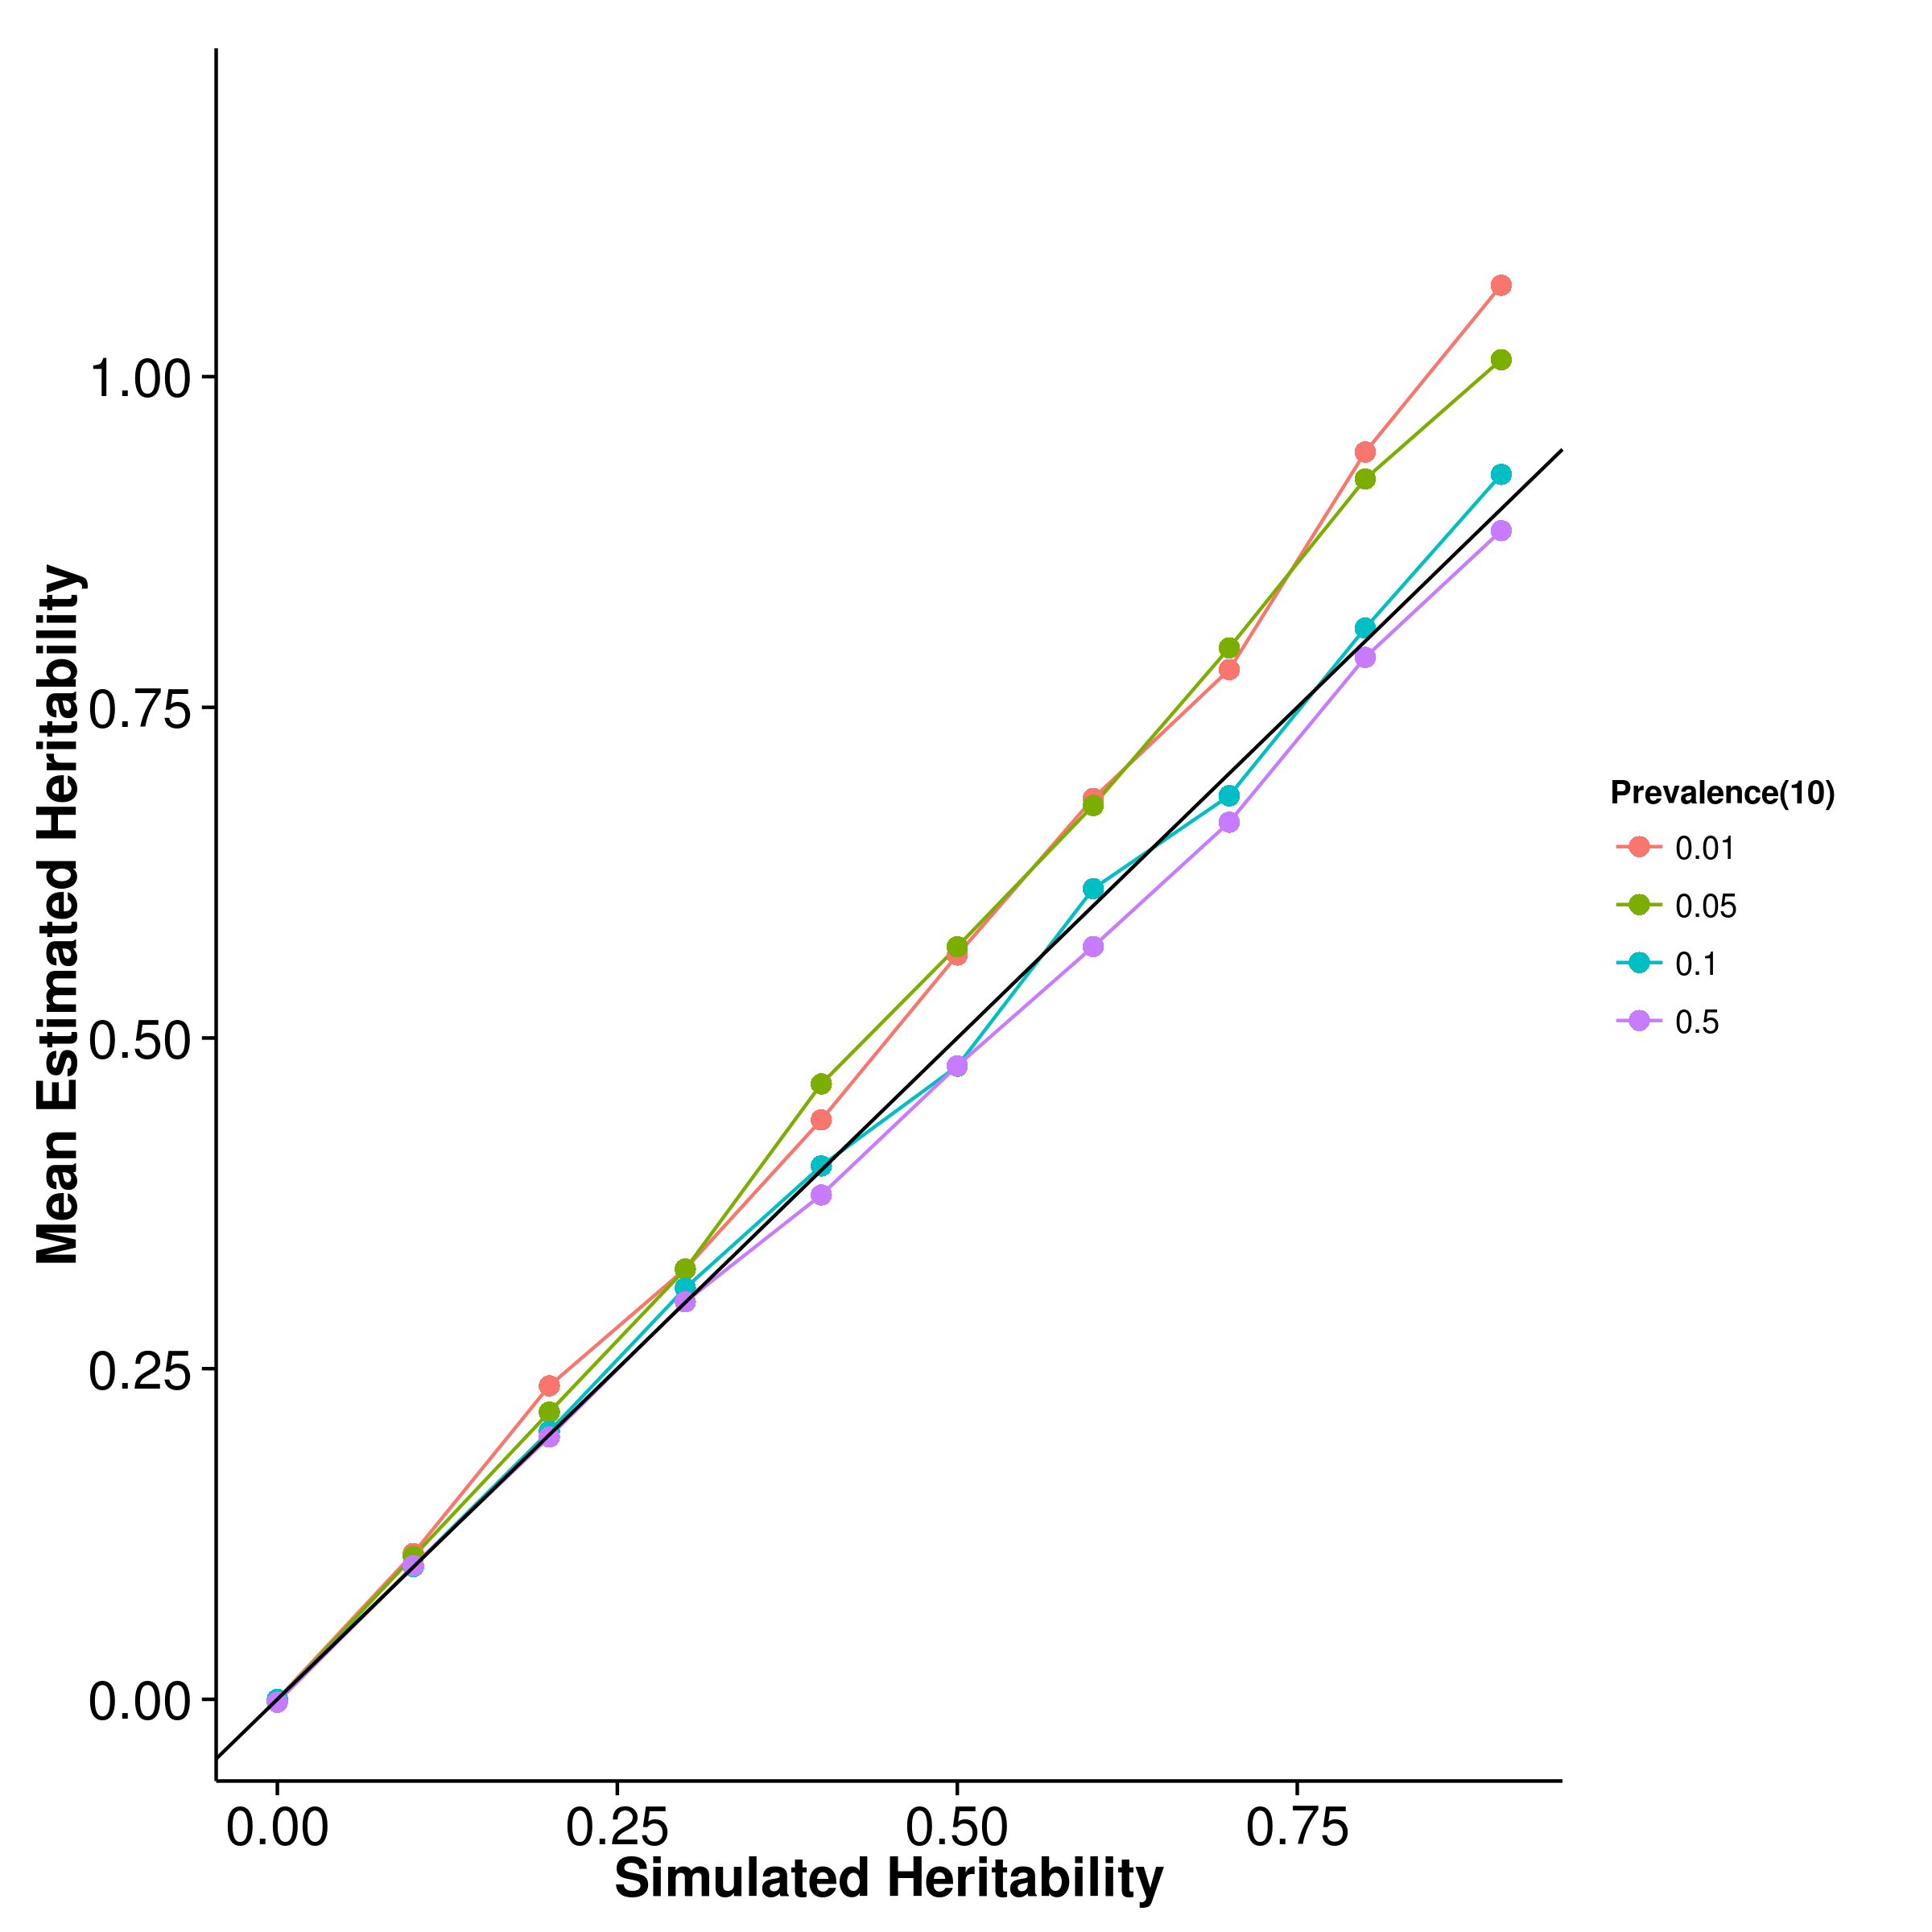
\includegraphics{figure/he_summary/cc_10c/shrek_CC_Rand_mean.png}}
					\label{fig:shrekCC10RandMean}
				}
				\subfloat[GCTA]{
					\scalebox{.4}{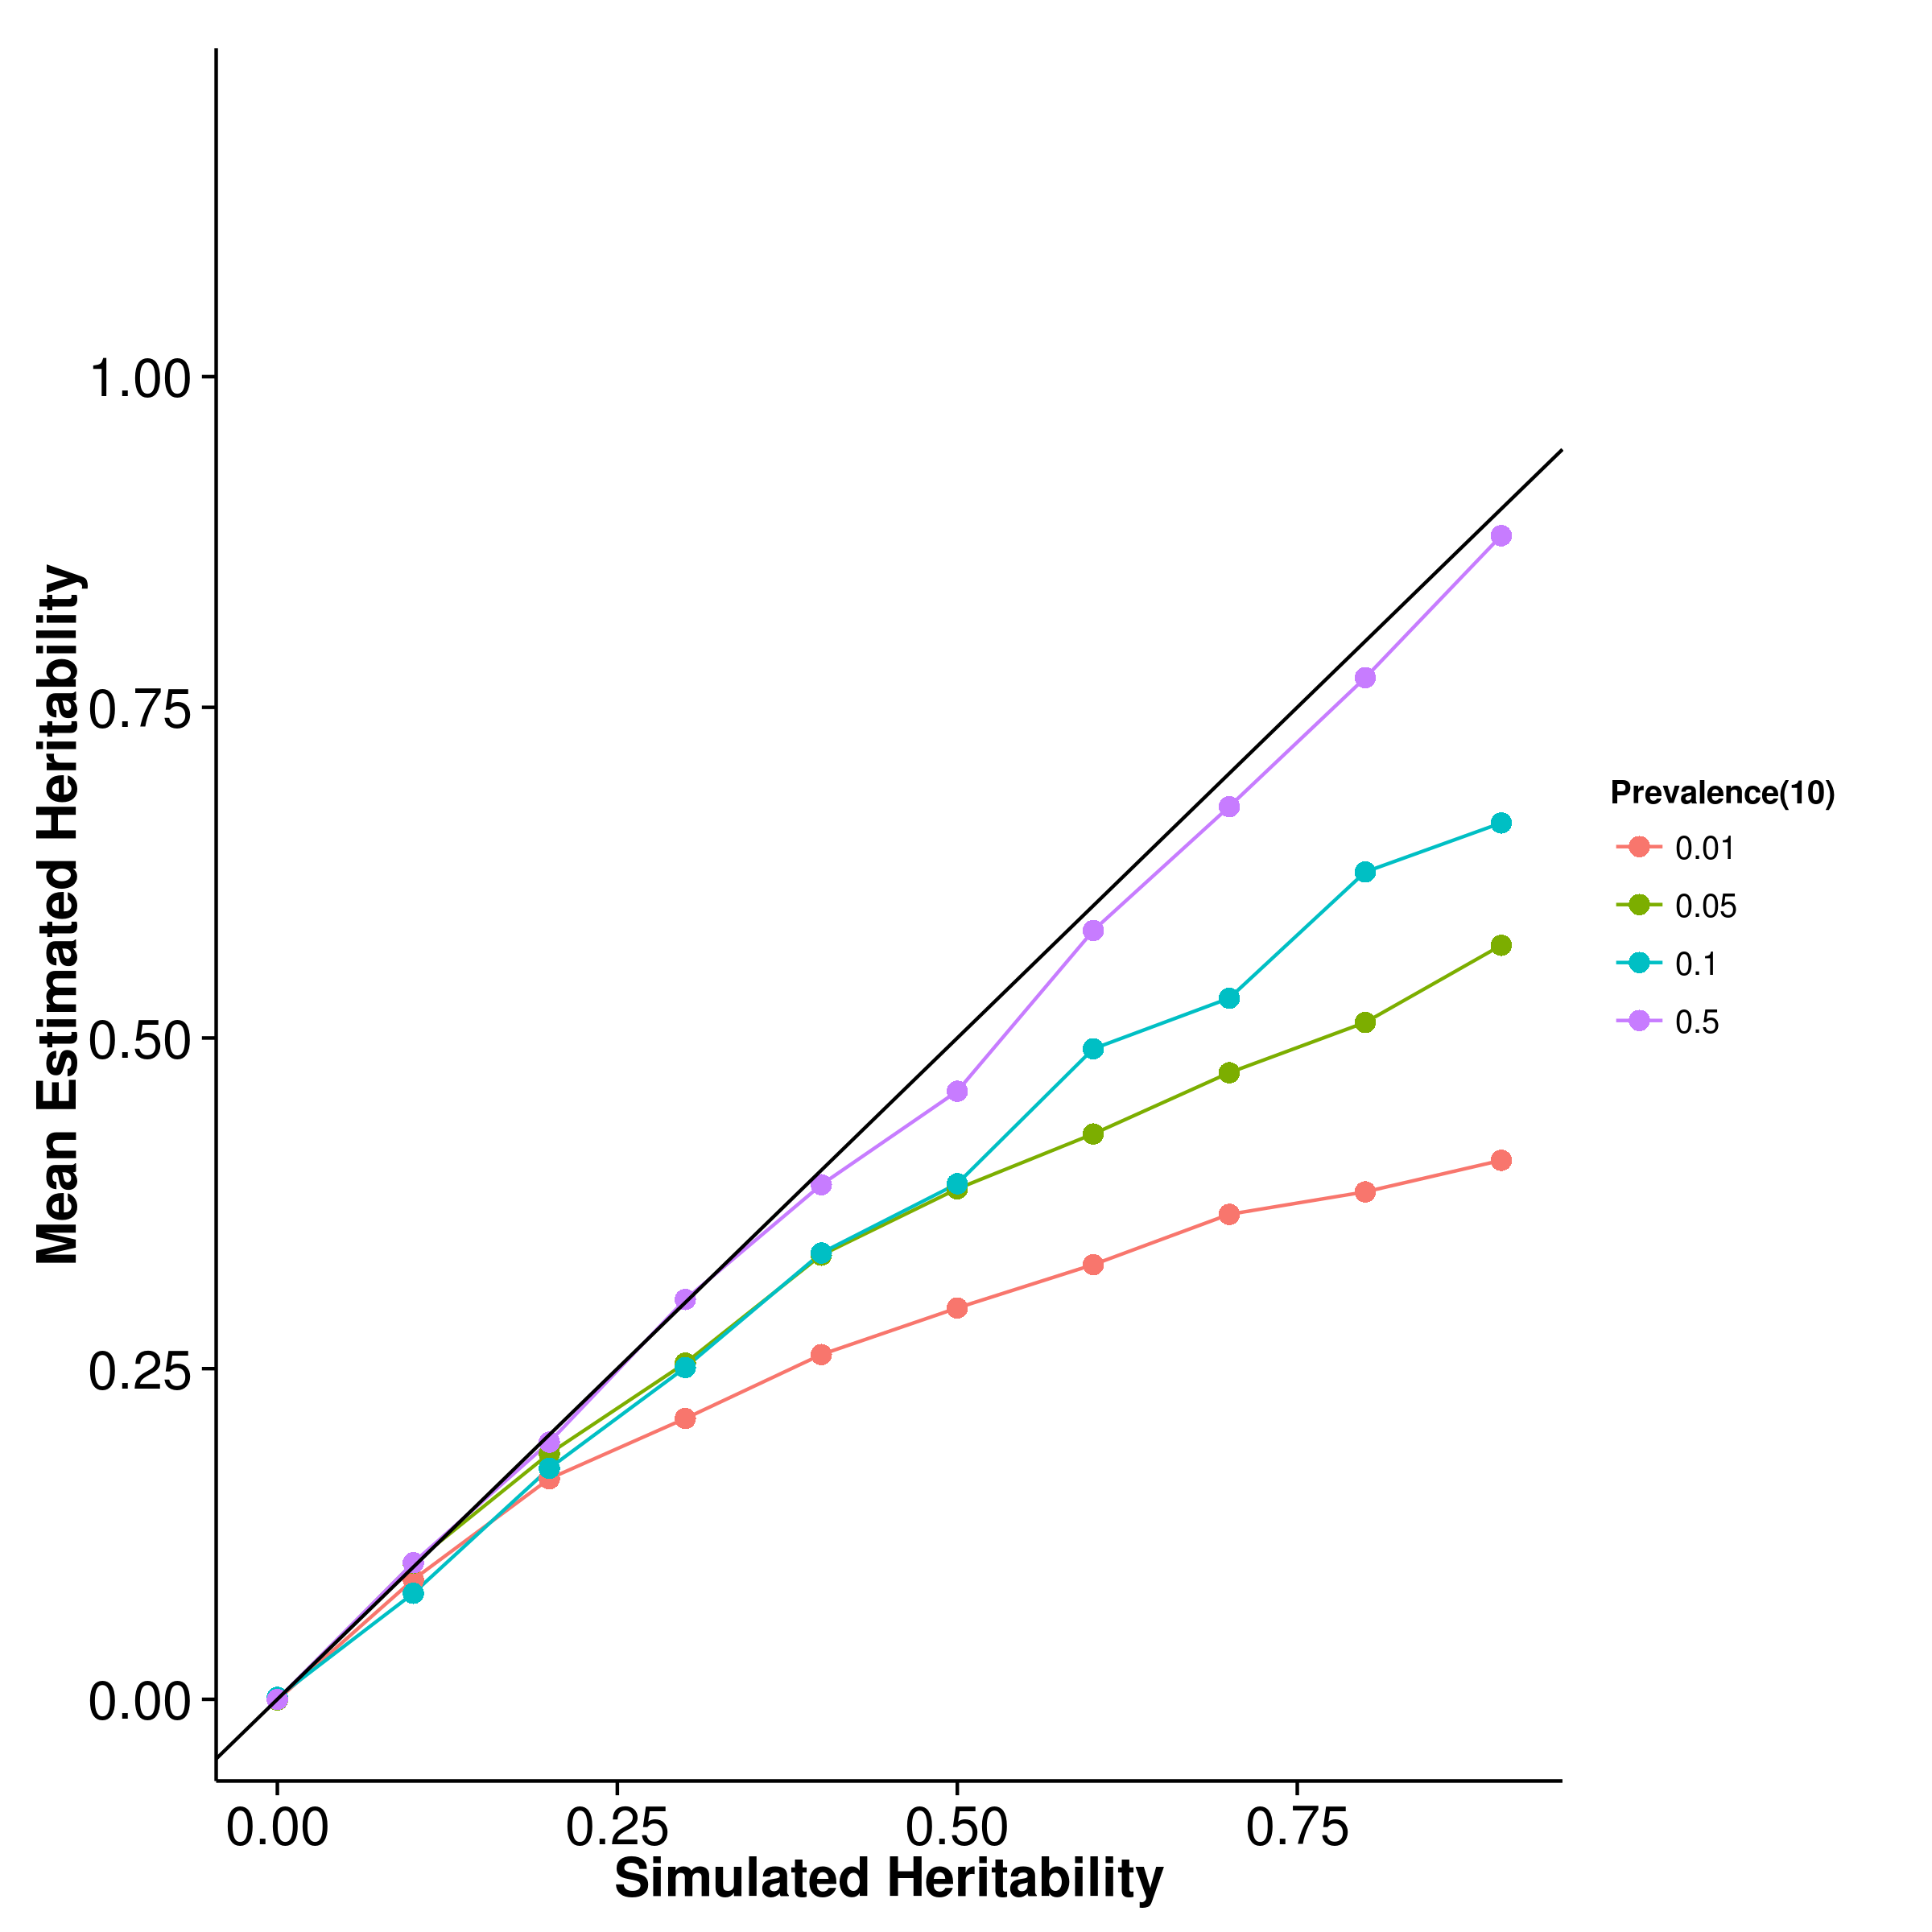
\includegraphics{figure/he_summary/cc_10c/gcta_CC_Rand_mean.png}}
					\label{fig:gctaCC10RandMean}
				}\\
				\subfloat[LDSC with fix intercept]{
					\scalebox{.4}{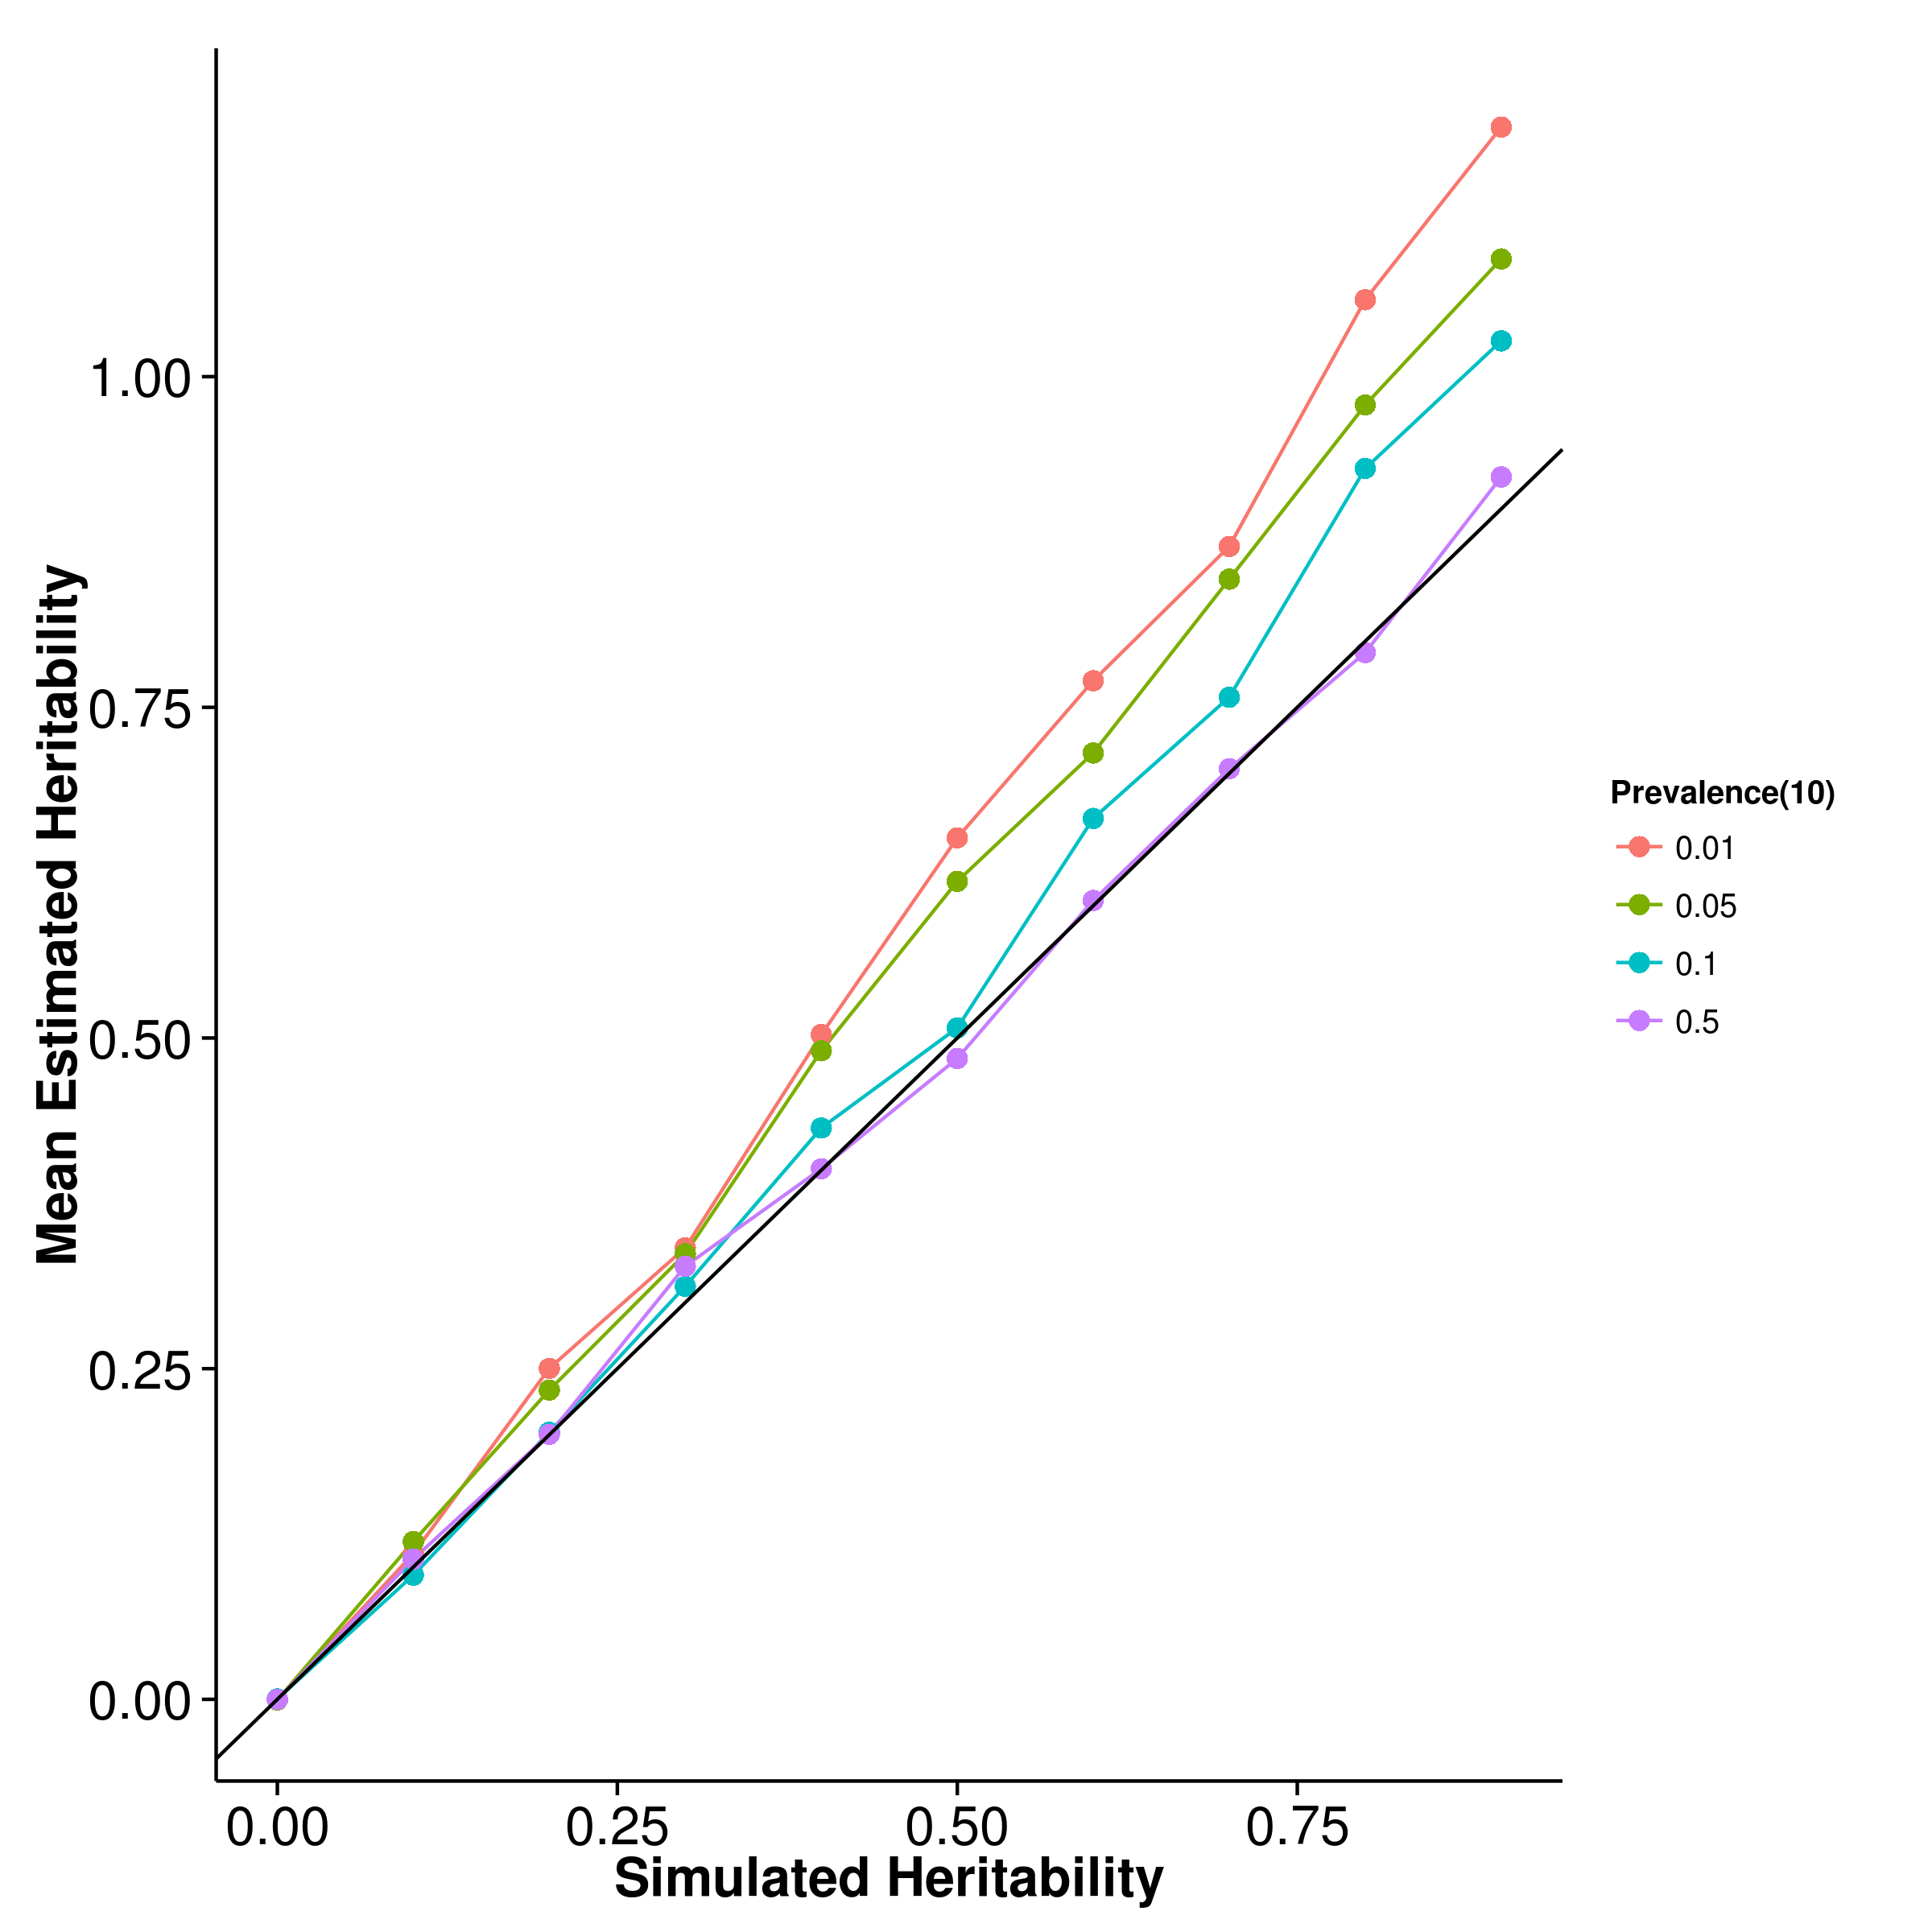
\includegraphics{figure/he_summary/cc_10c/ldsc_CC_Rand_mean.png}}
					\label{fig:ldscCC10RandMean}
				}
				\subfloat[LDSC with intercept estimation]{
					
					\scalebox{.4}{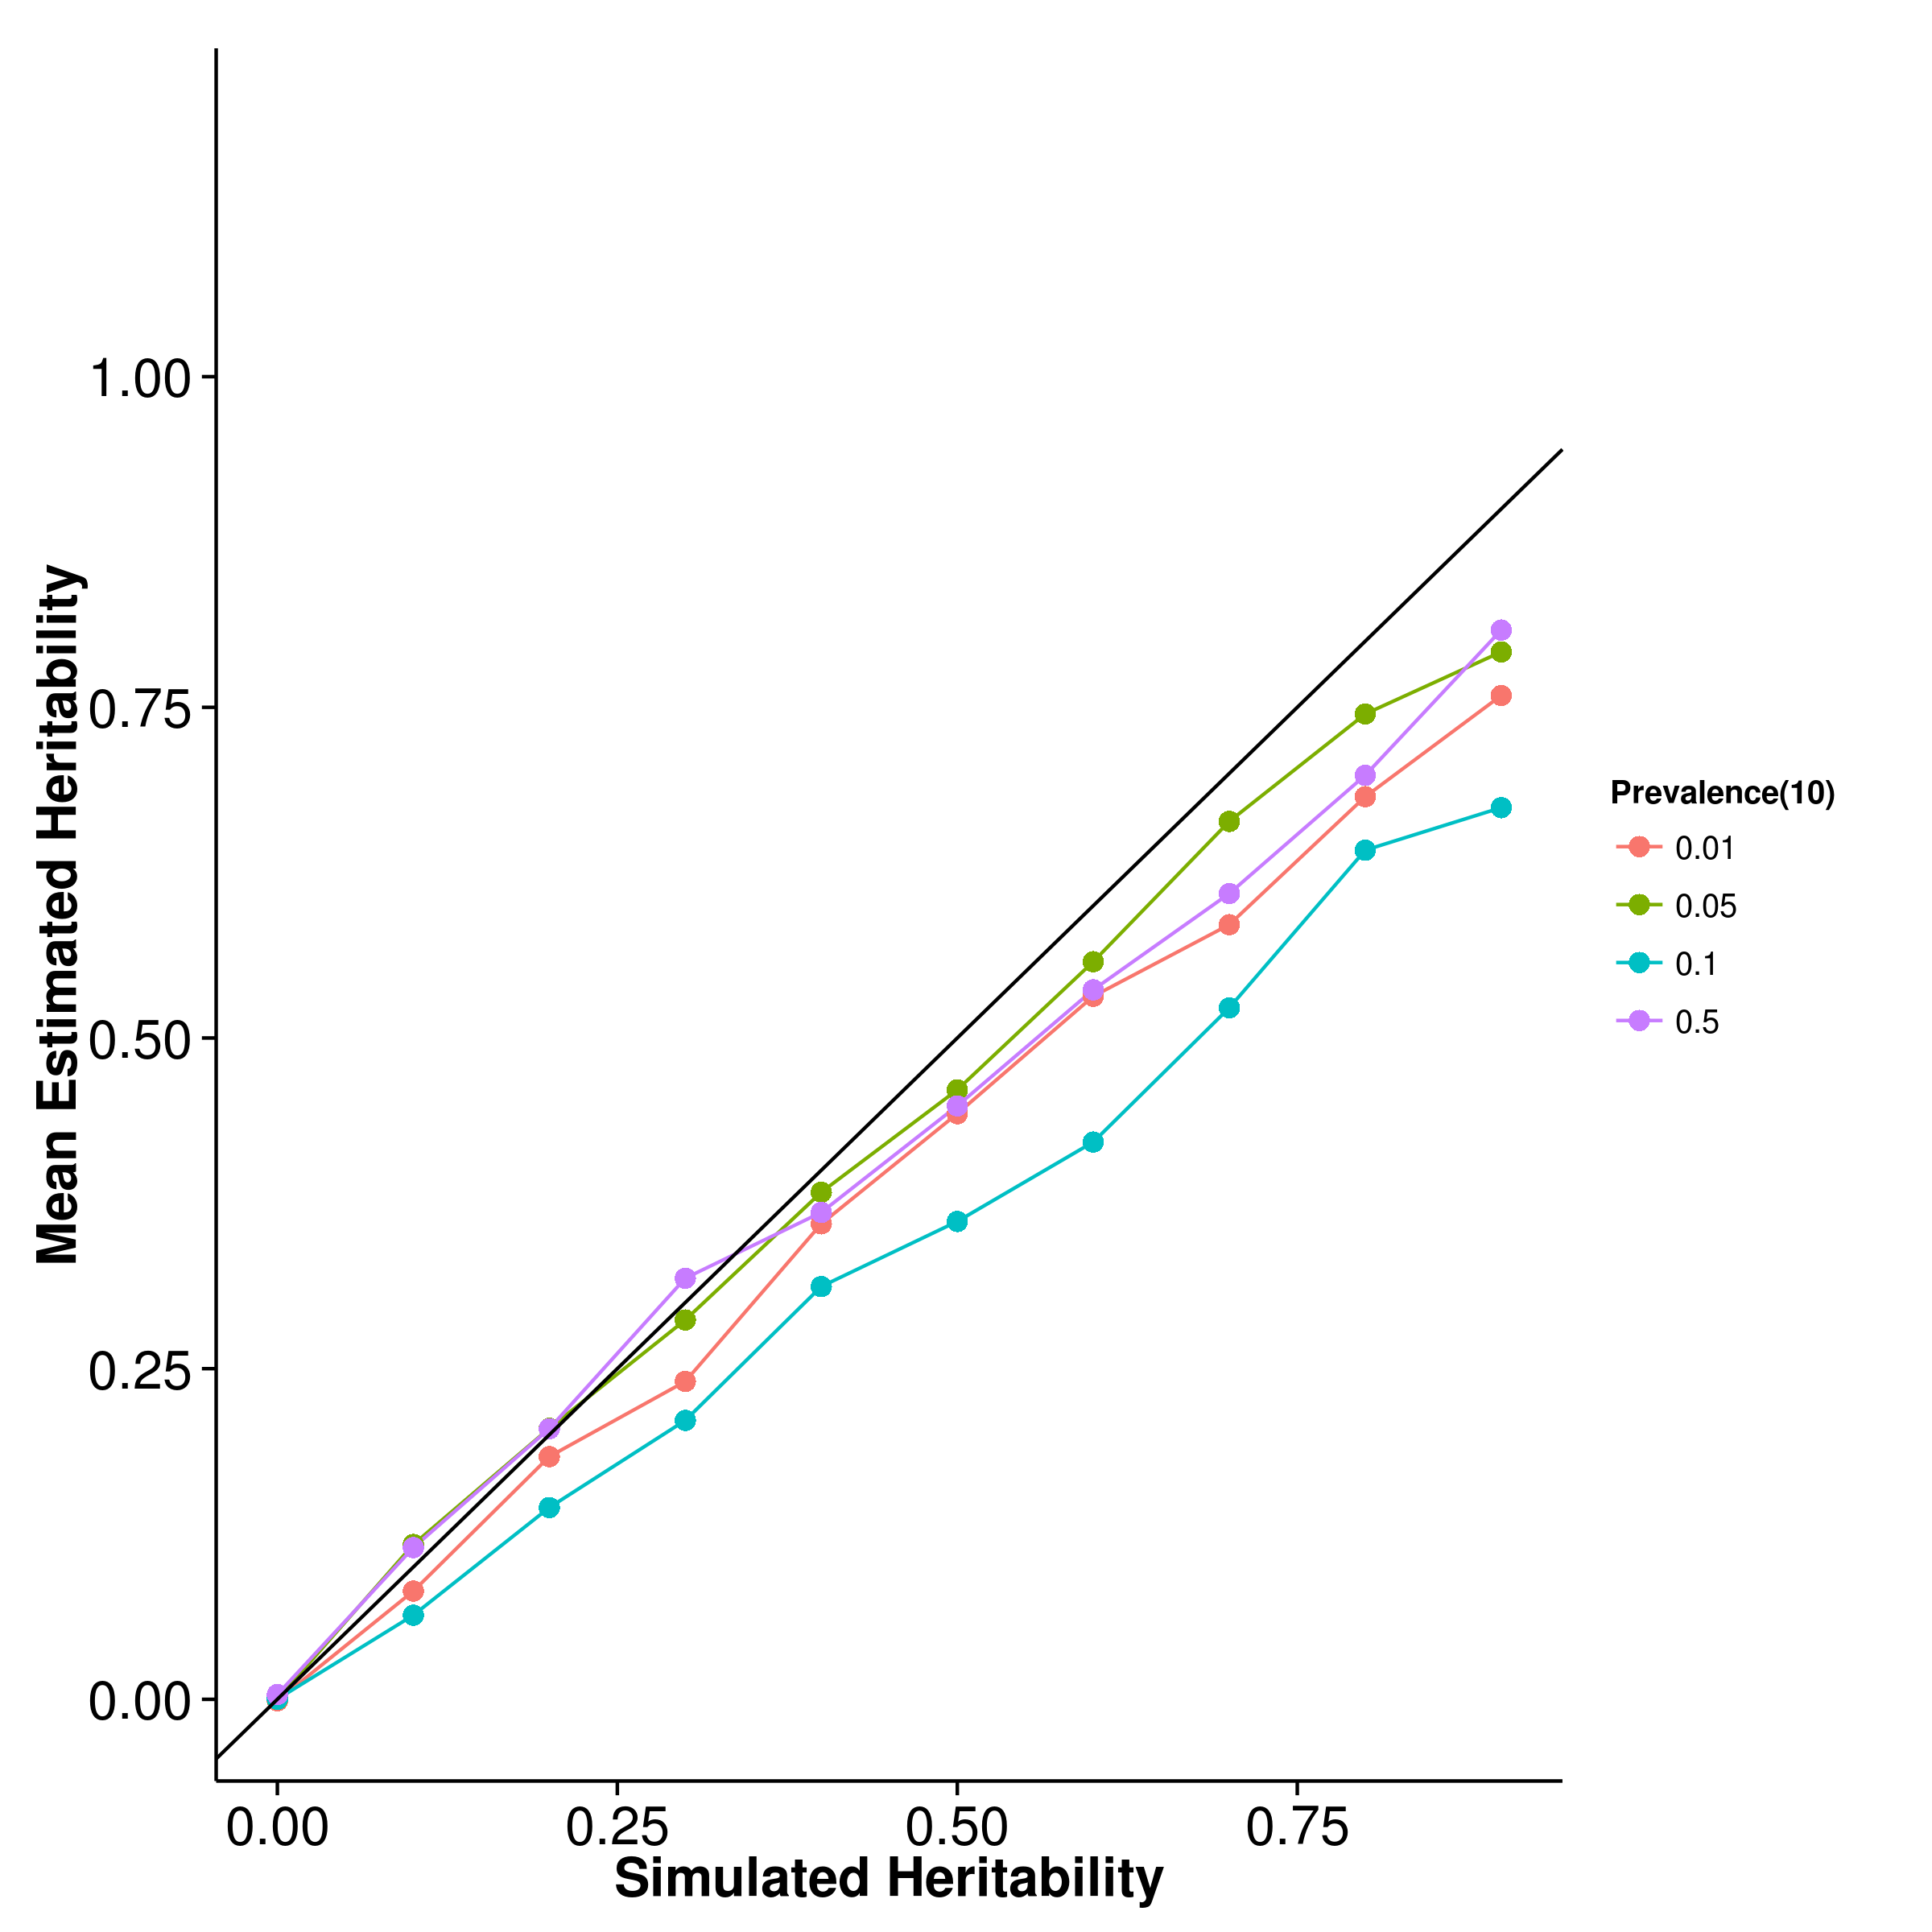
\includegraphics{figure/he_summary/cc_10c/ldscIn_CC_Rand_mean.png}}
					\label{fig:ldscInCC10RandMean}
				}
				\caption[Mean of Case Control Simulation Results (10 Causal)]
				{Mean of results from case control simulation with random effect size simulation with 10 causal \glspl{SNP}.
					The performance of \gls{gcta} was as suggested by \citet{Golan2014} where there was an underestimation as prevalence decreases.
					On the other hand, the upward bias of both \gls{ldsc} with fixed intercept and \gls{shrek} increases as the prevalence decreases whereas \gls{ldsc} with intercept estimation seems relatively robust to the change in prevalence.
				} 
				\label{fig:CC10RandMean}
			\end{figure}
			%Empirical Variance
			\begin{figure}
				\centering
				\subfloat[SHREK]{
					\scalebox{.4}{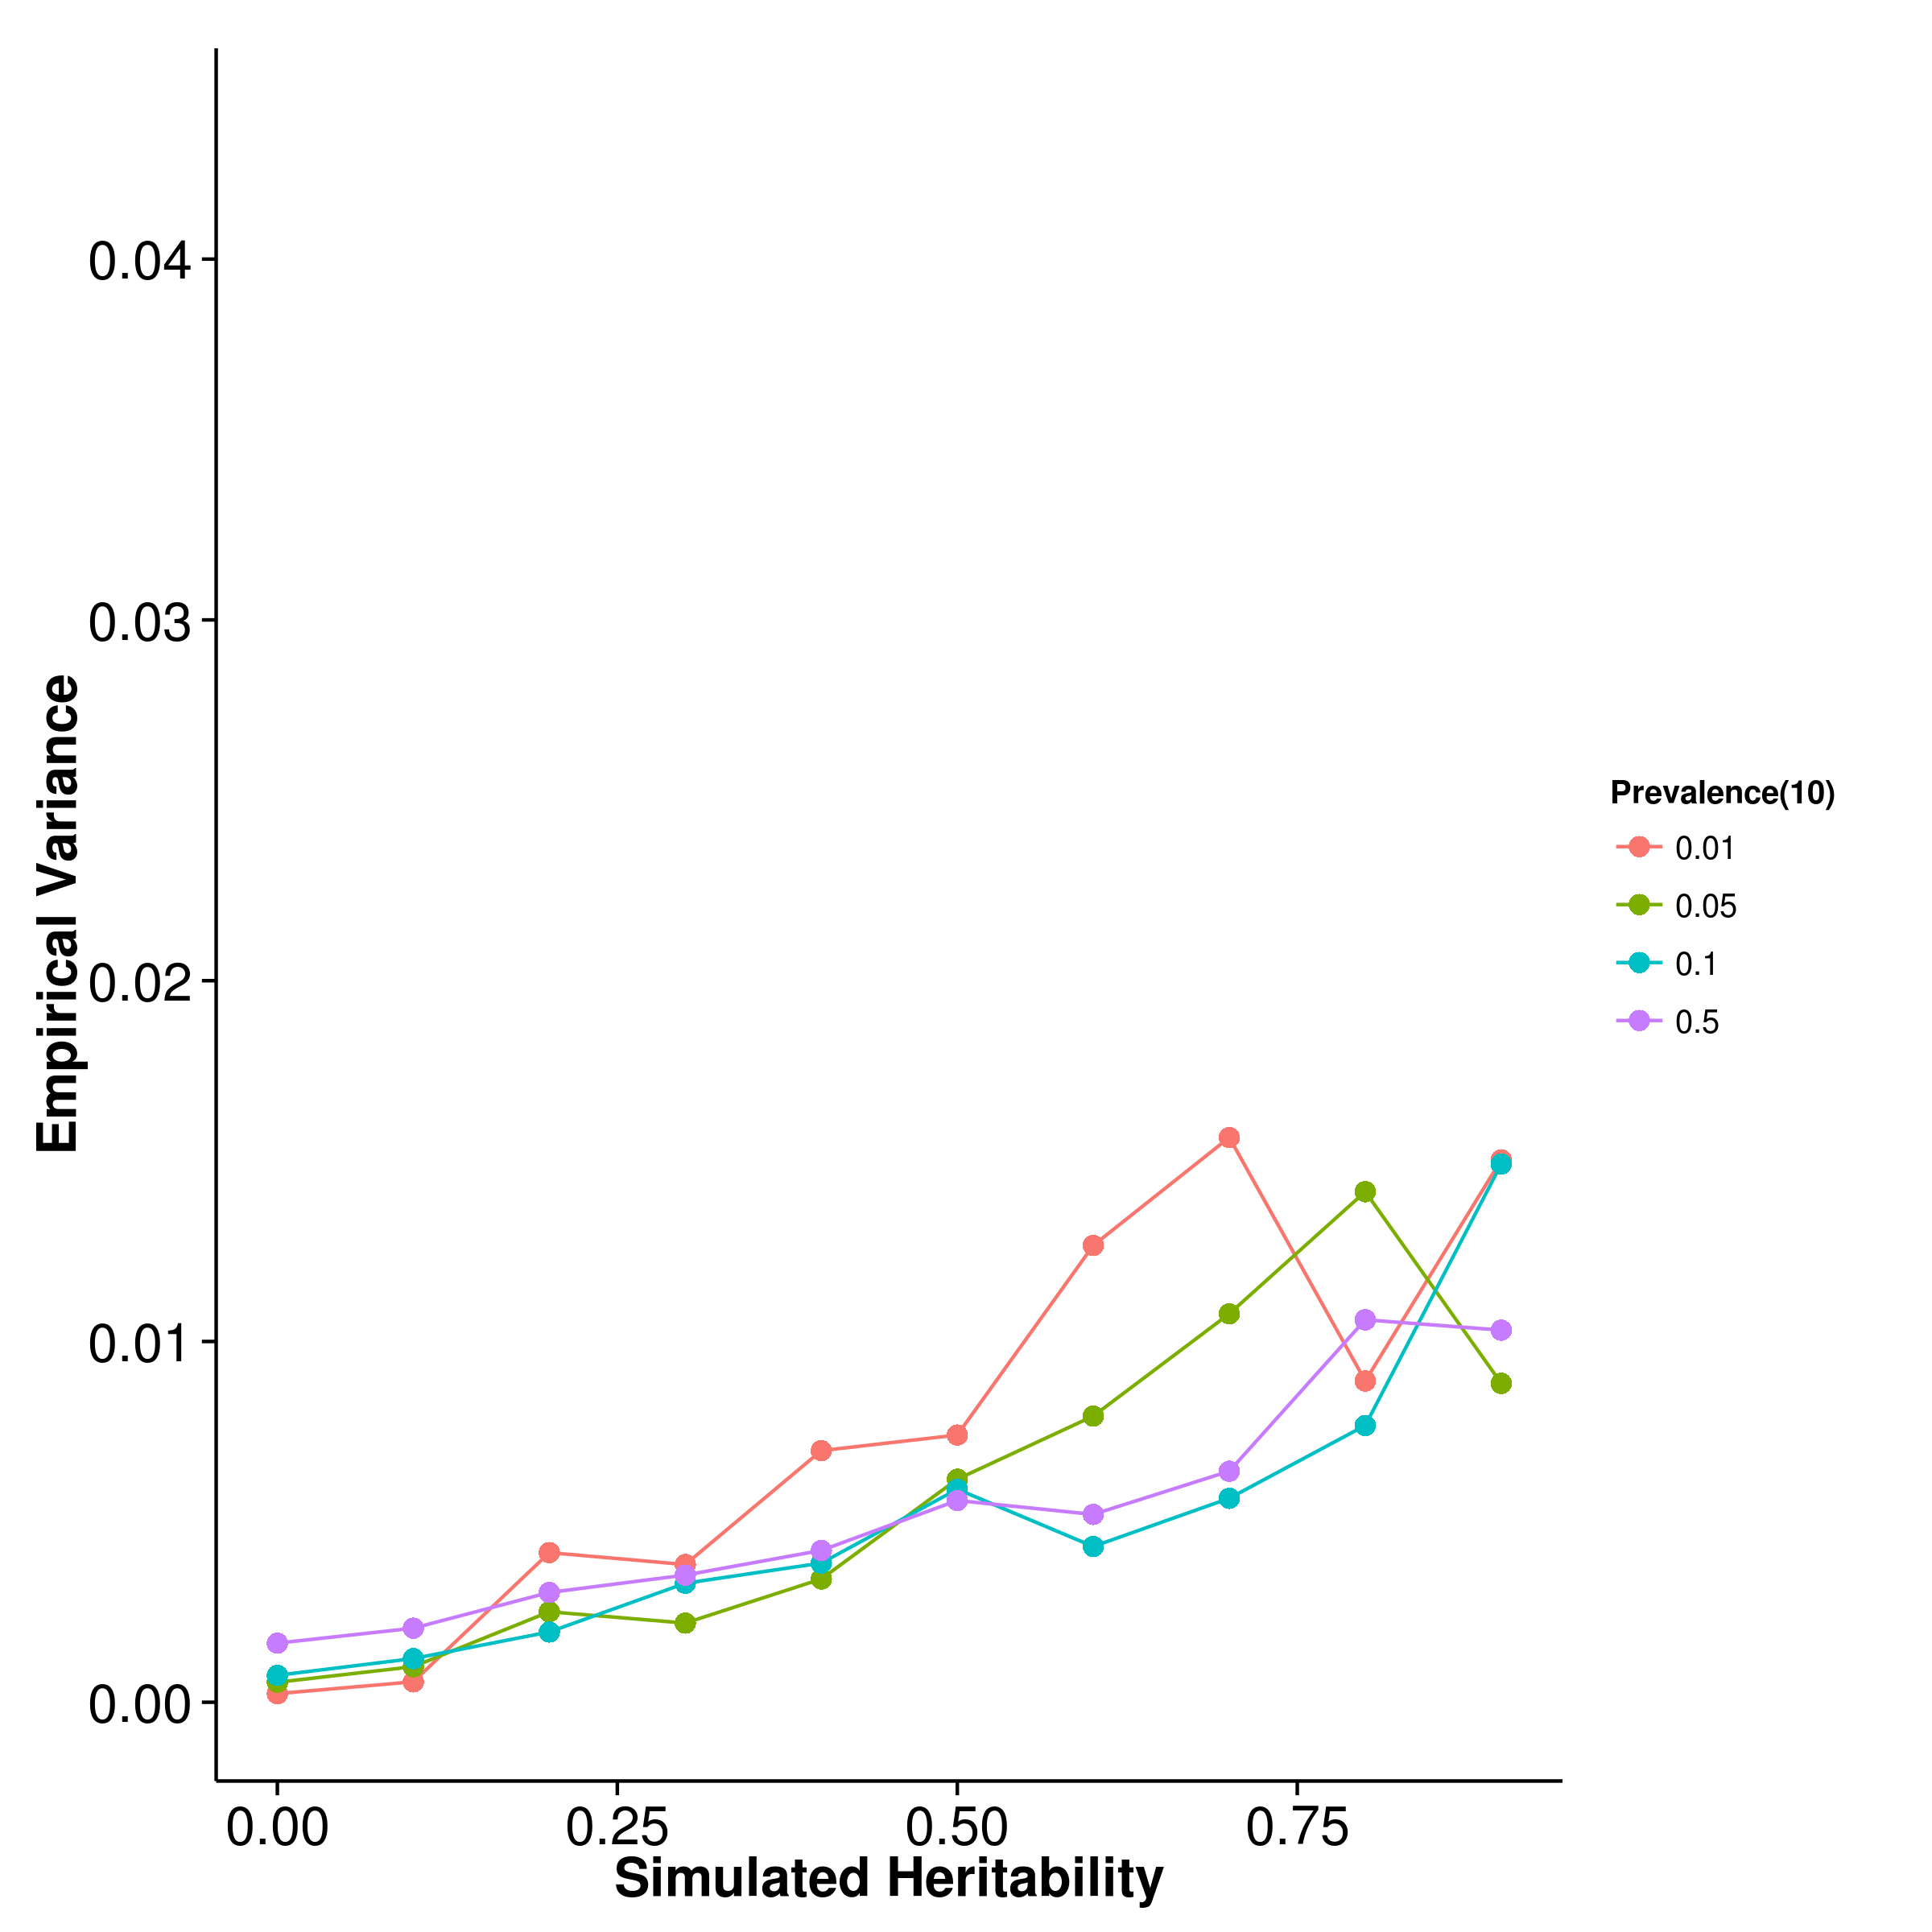
\includegraphics{figure/he_summary/cc_10c/shrek_CC_Rand_sd.png}}
					\label{fig:shrekCC10RandVar}
				}
				\subfloat[GCTA]{
					\scalebox{.4}{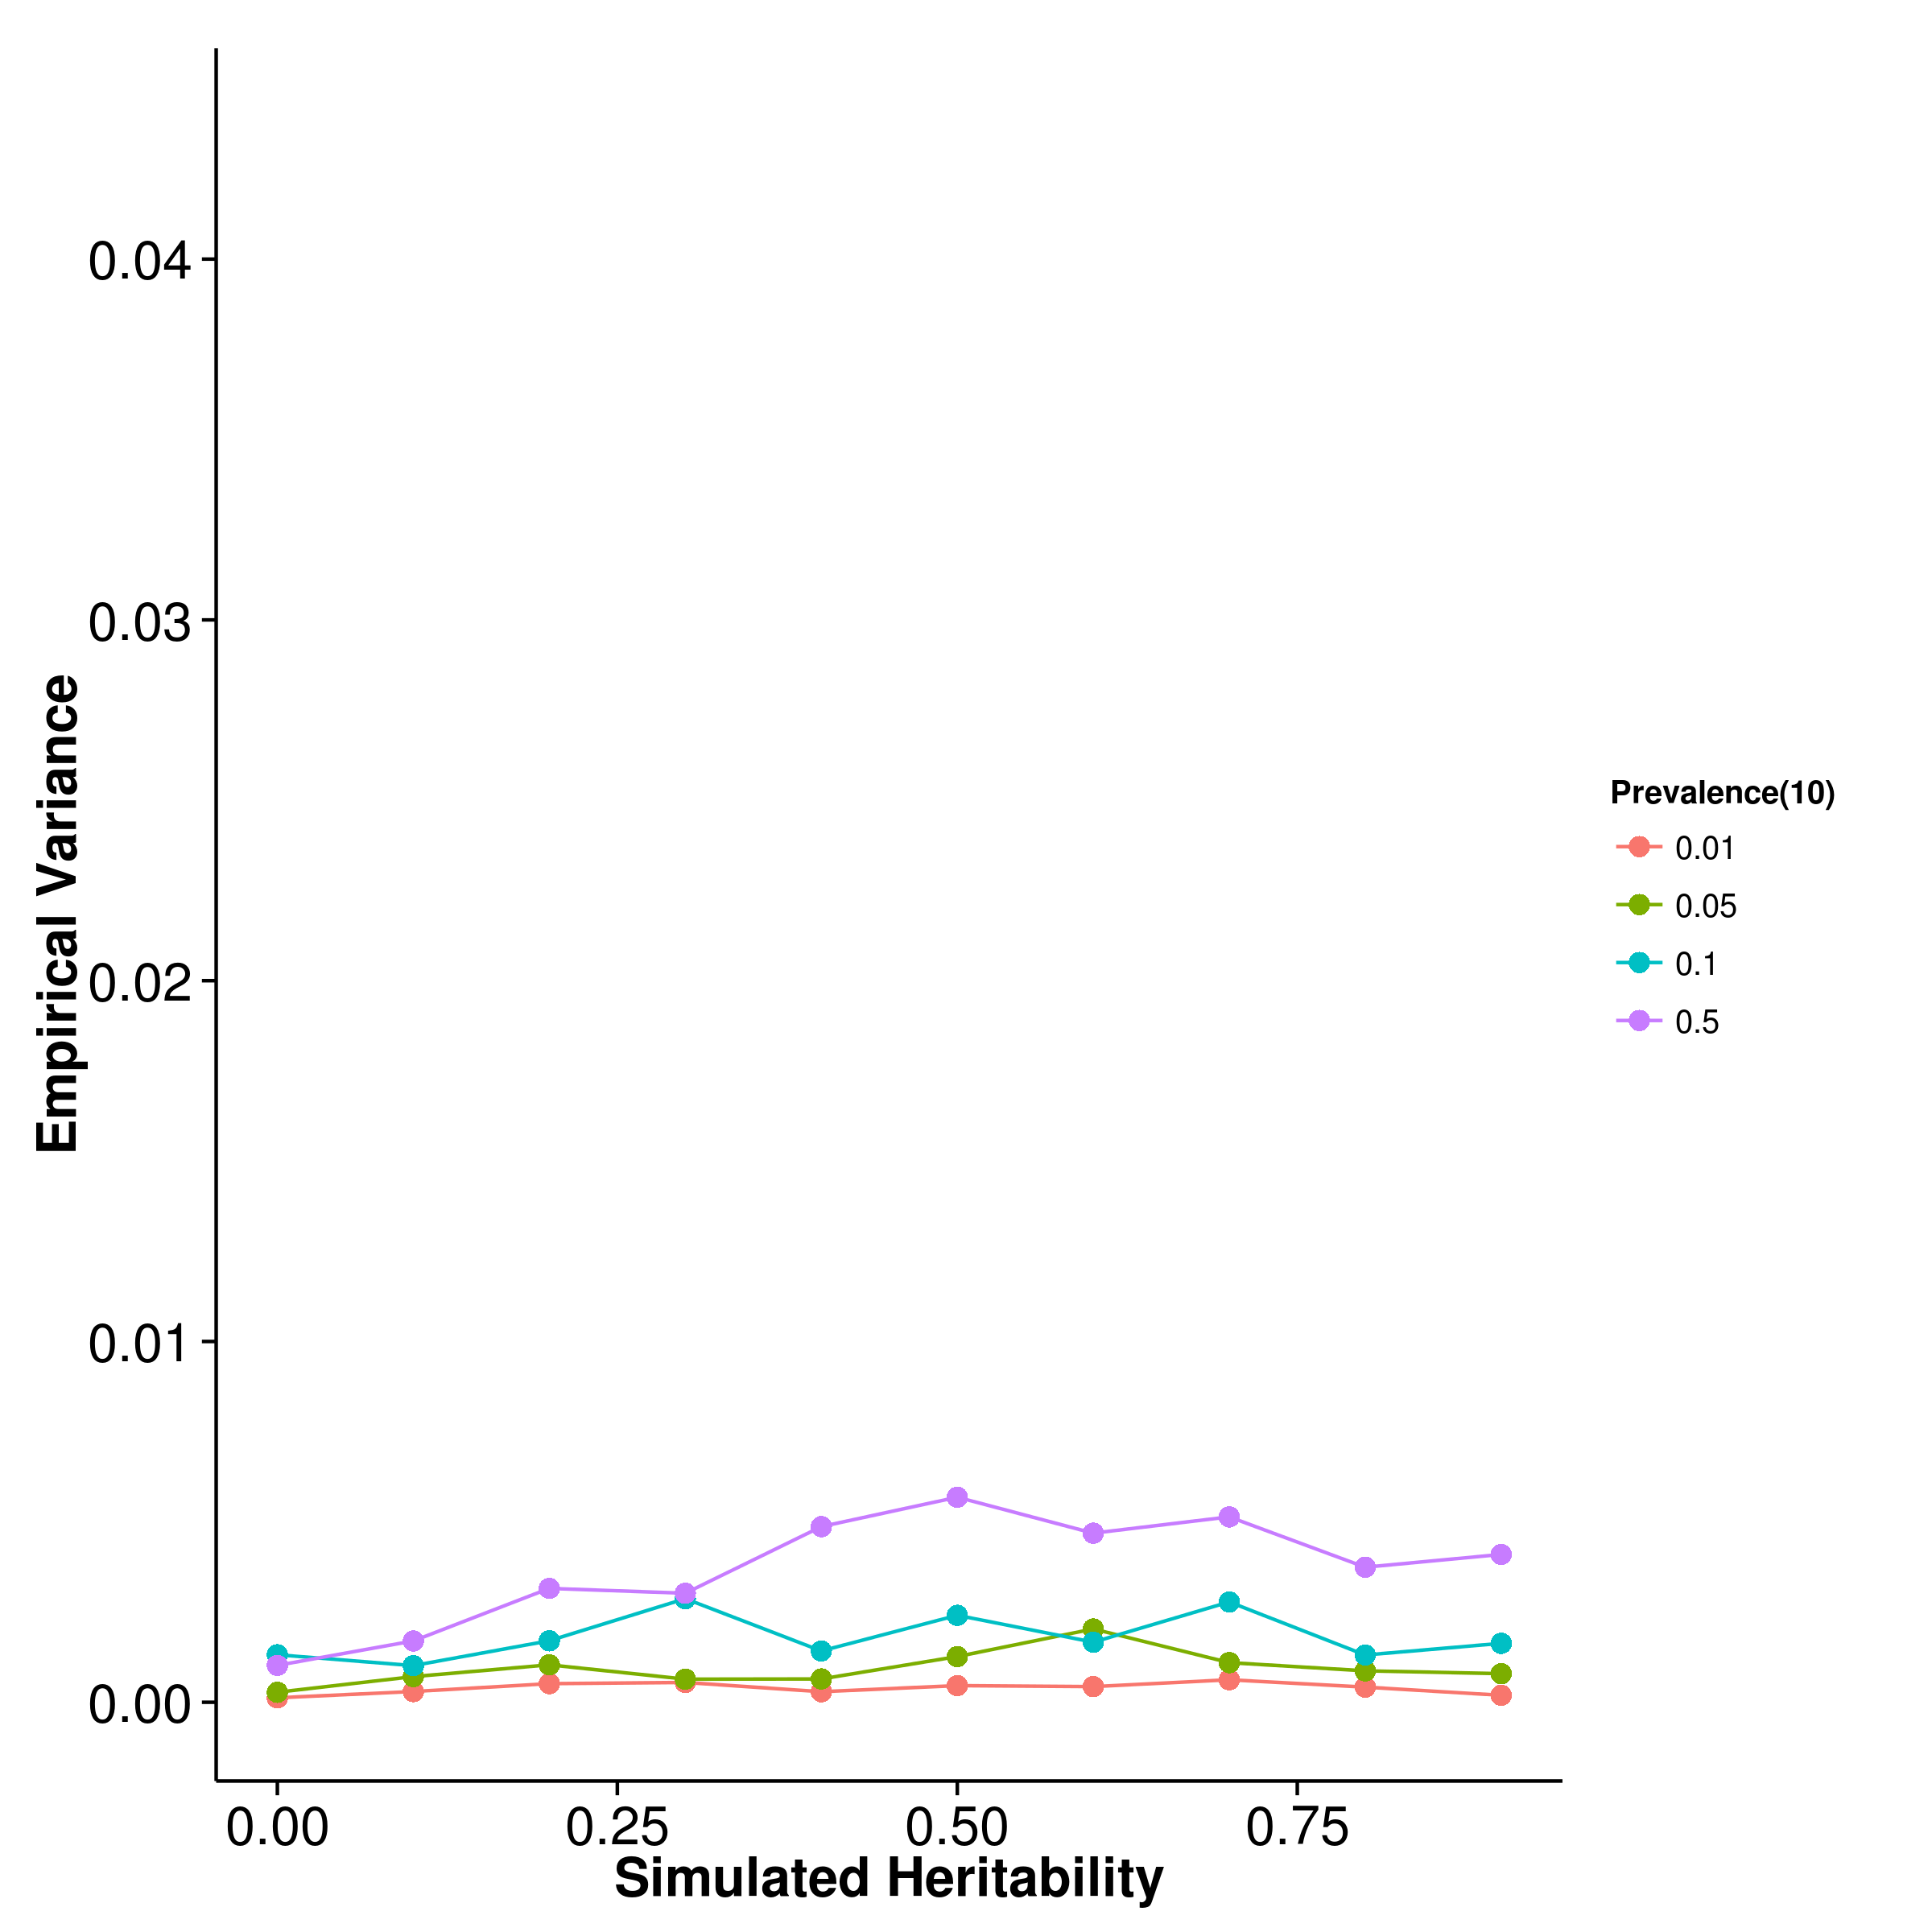
\includegraphics{figure/he_summary/cc_10c/gcta_CC_Rand_sd.png}}
					\label{fig:gctaCC10RandVar}
				}\\
				\subfloat[LDSC with fix intercept]{
					\scalebox{.4}{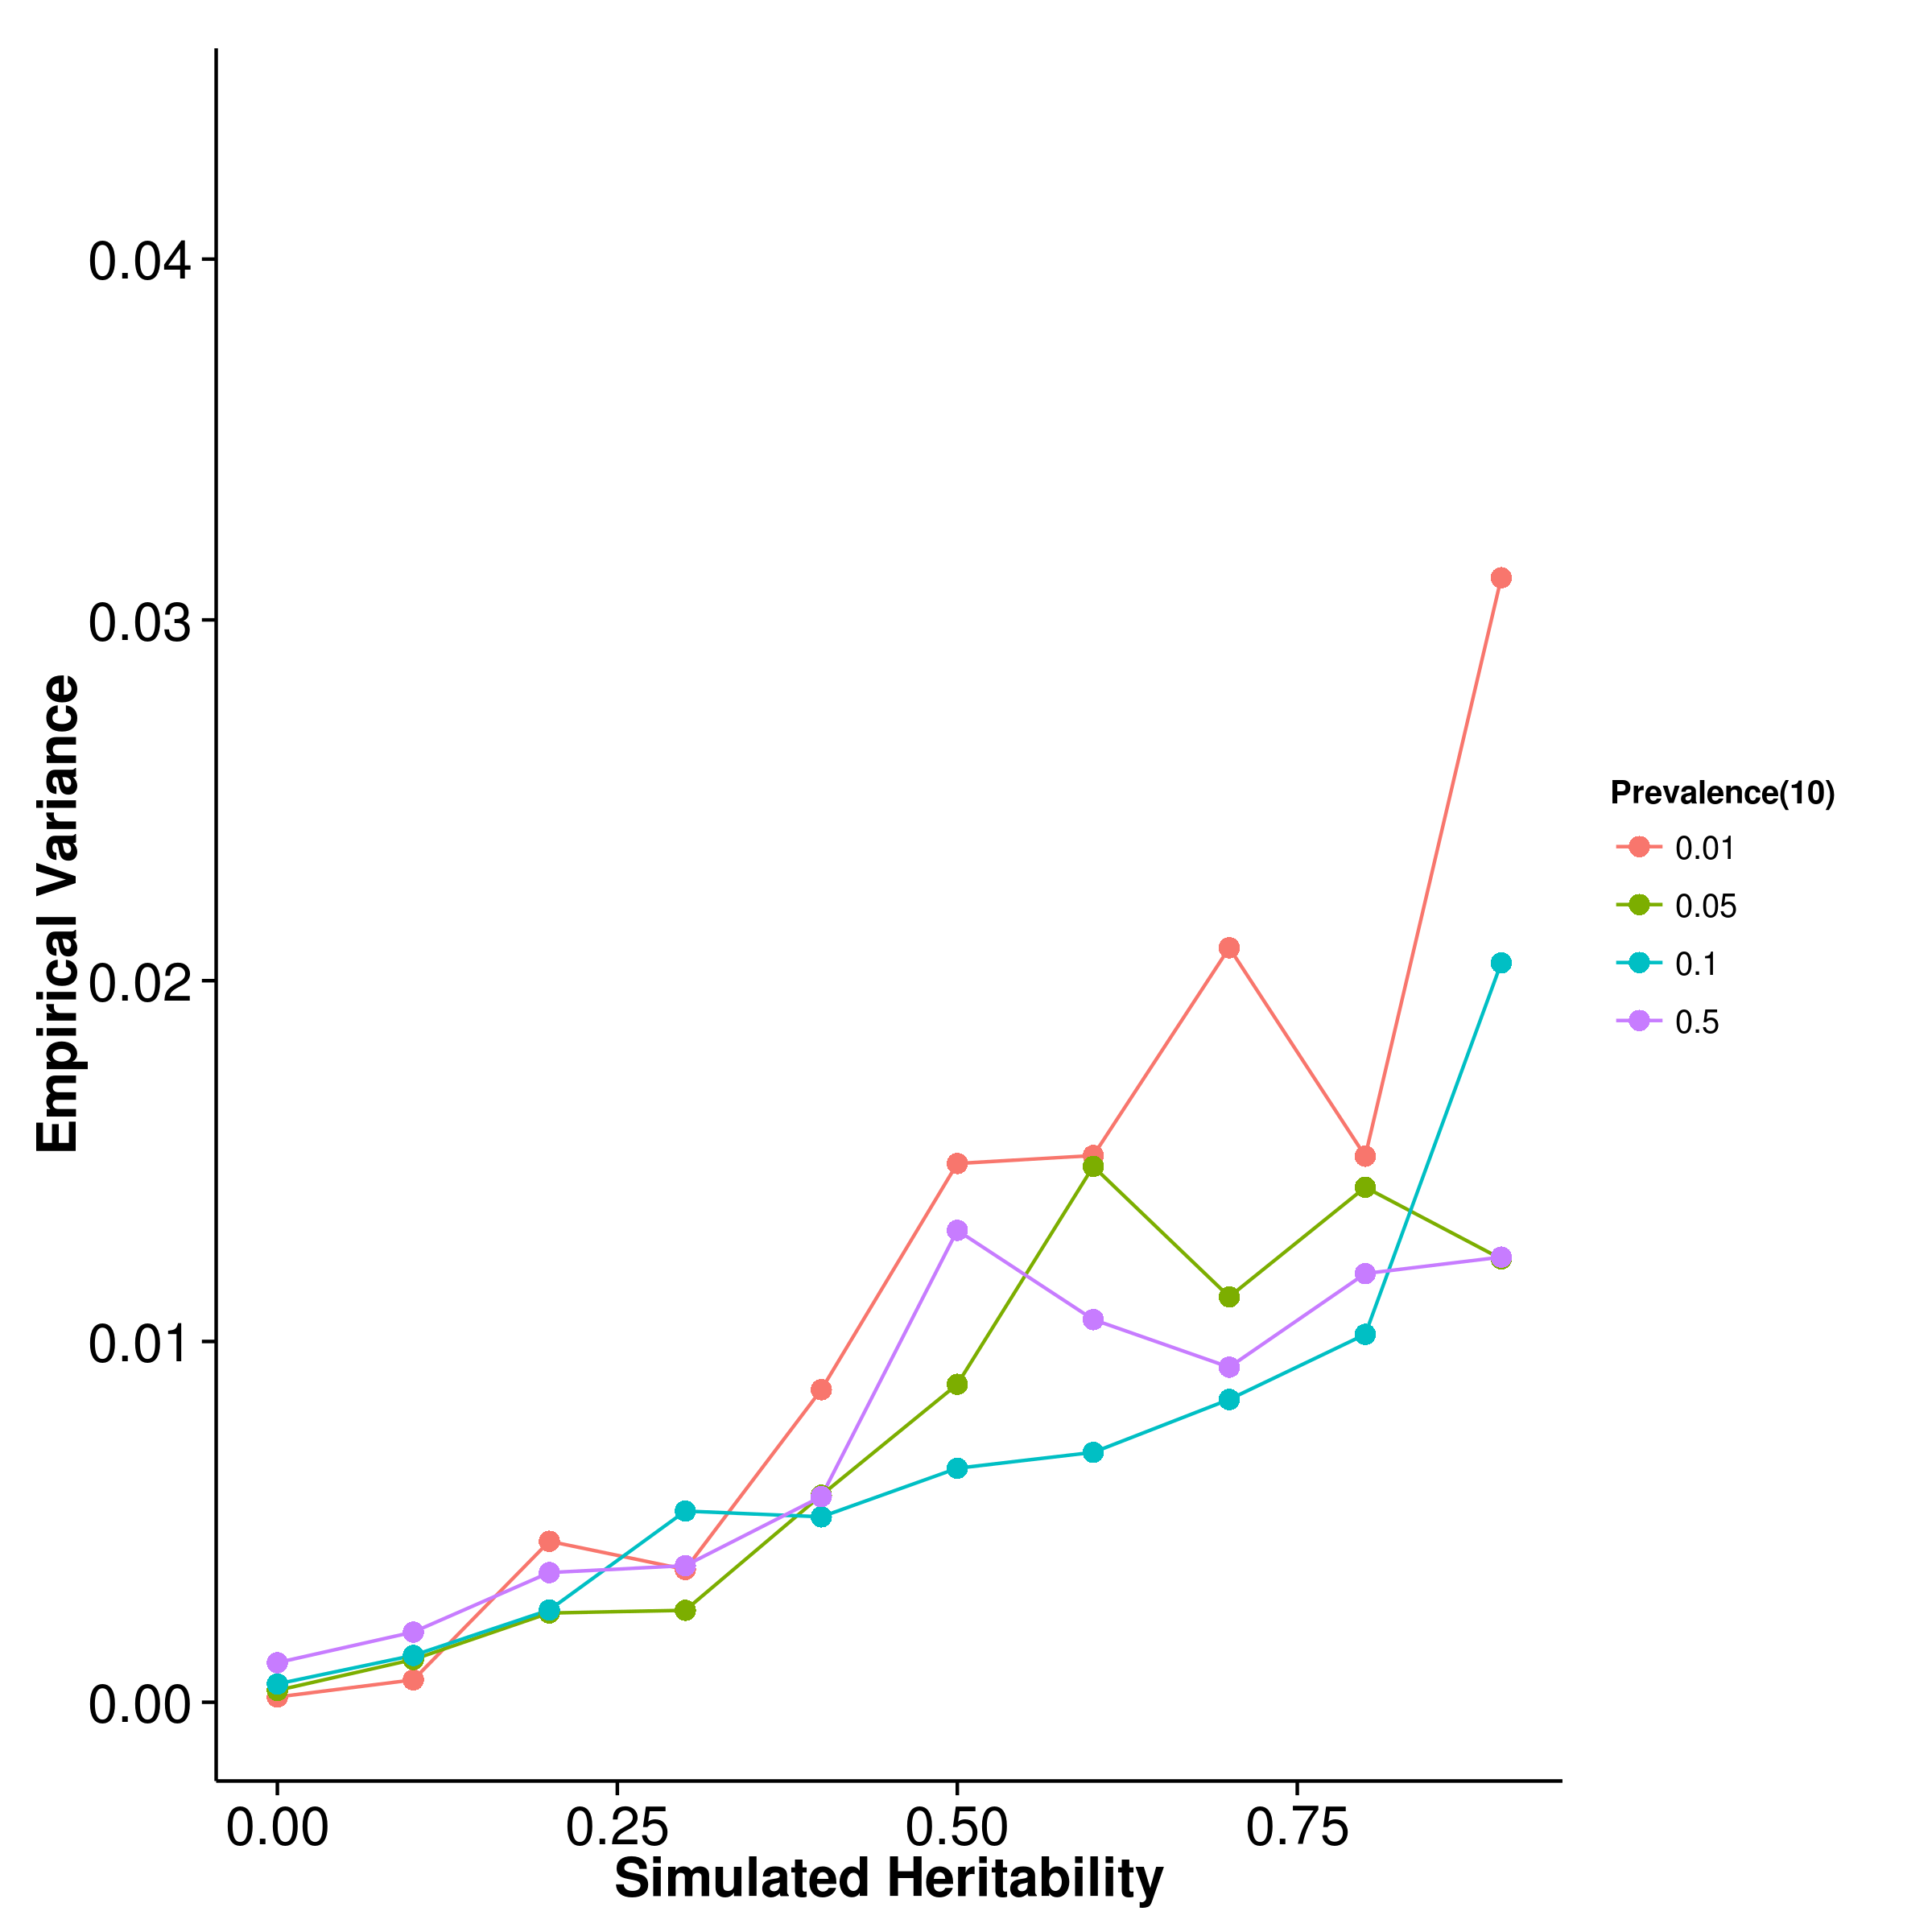
\includegraphics{figure/he_summary/cc_10c/ldsc_CC_Rand_sd.png}}
					\label{fig:ldscCC10RandVar}
				}
				\subfloat[LDSC with intercept estimation]{
					
					\scalebox{.4}{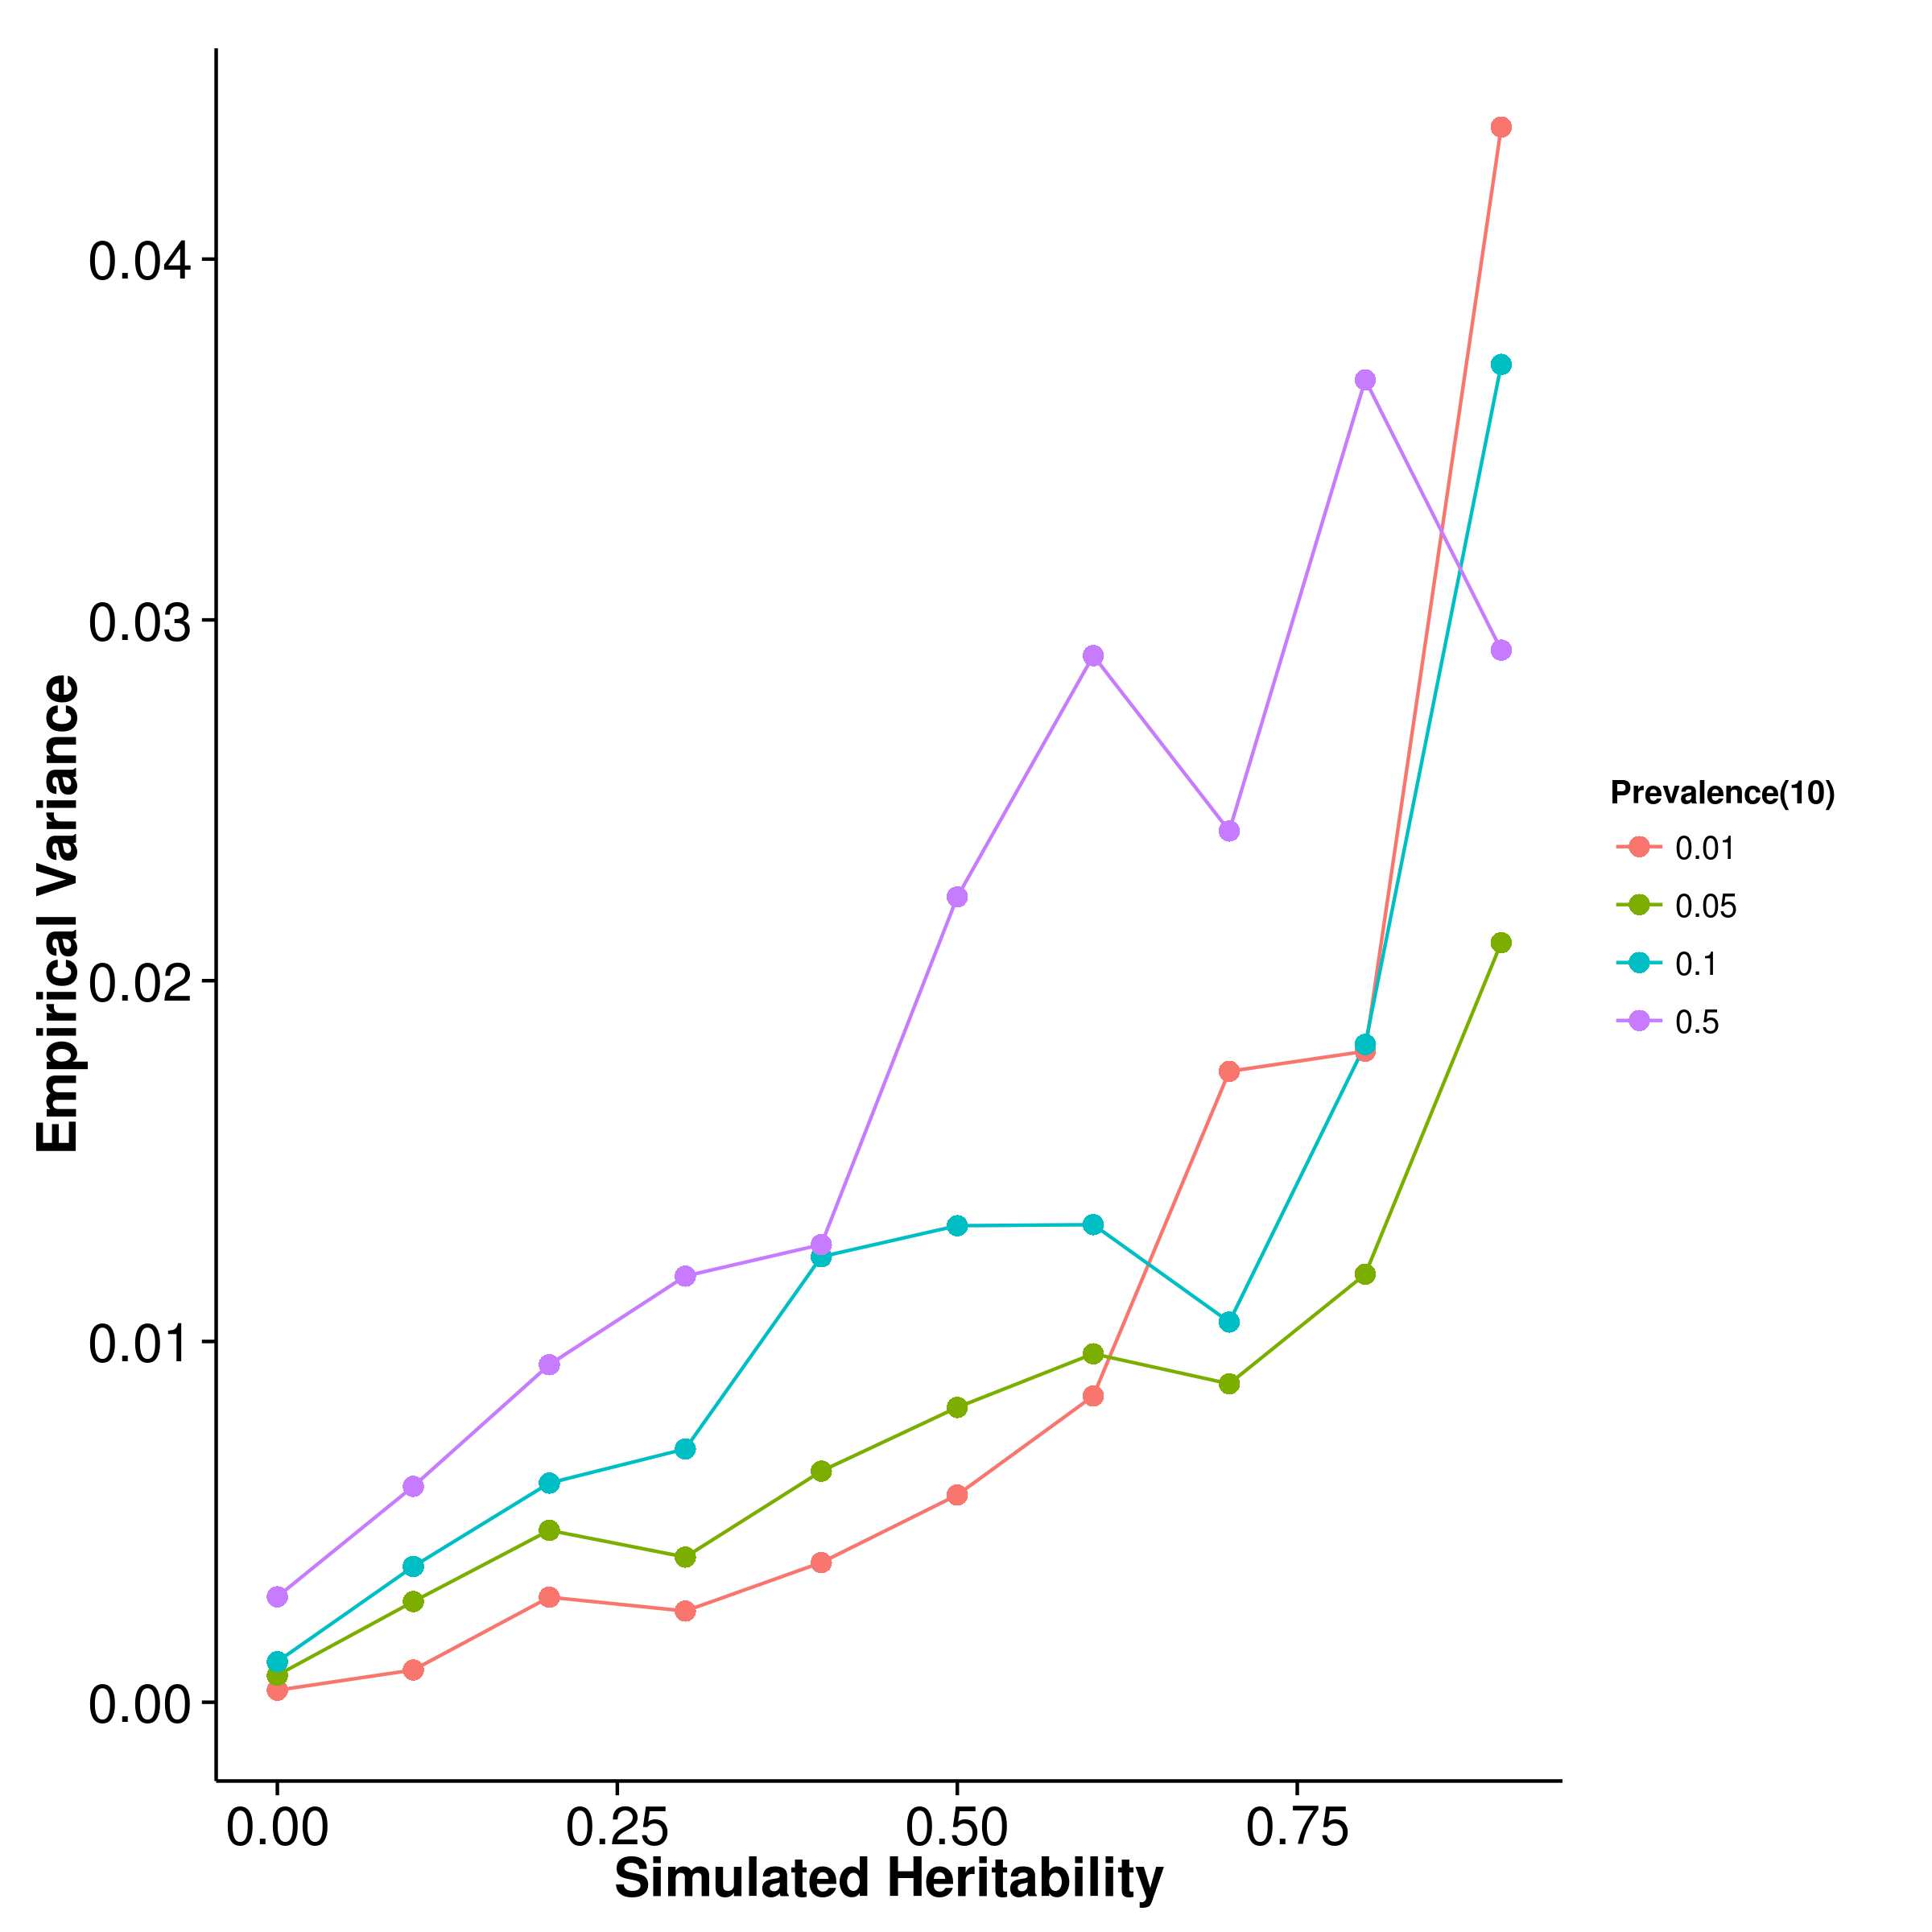
\includegraphics{figure/he_summary/cc_10c/ldscIn_CC_Rand_sd.png}}
					\label{fig:ldscInCC10RandVar}
				}
				\caption[Variance of Case Control Simulation Results (10 Causal)]
				{Variance of results from case control simulation with random effect size simulation with 10 causal \glspl{SNP}.
					There were no clear pattern as to how the prevalence affect the empirical variance of estimates from \gls{shrek} and \gls{ldsc}. 
					For \gls{gcta}, it seems like a larger prevalence tends to result in a larger empirical variance. 
					Again, \gls{gcta} has the lowest variance, follow by \gls{shrek} and \gls{ldsc} with fixed intercept.
					Nonetheless, it was important to remember that in case control simulation, a much smaller amount of \glspl{SNP} was used, thus the results was not directly comparable to results from the quantitative simulation.
				} 
				\label{fig:CC10RandVar}
			\end{figure}
			%Variance estimation			
			\begin{figure}
				\centering
				\subfloat[SHREK]{
					\scalebox{.4}{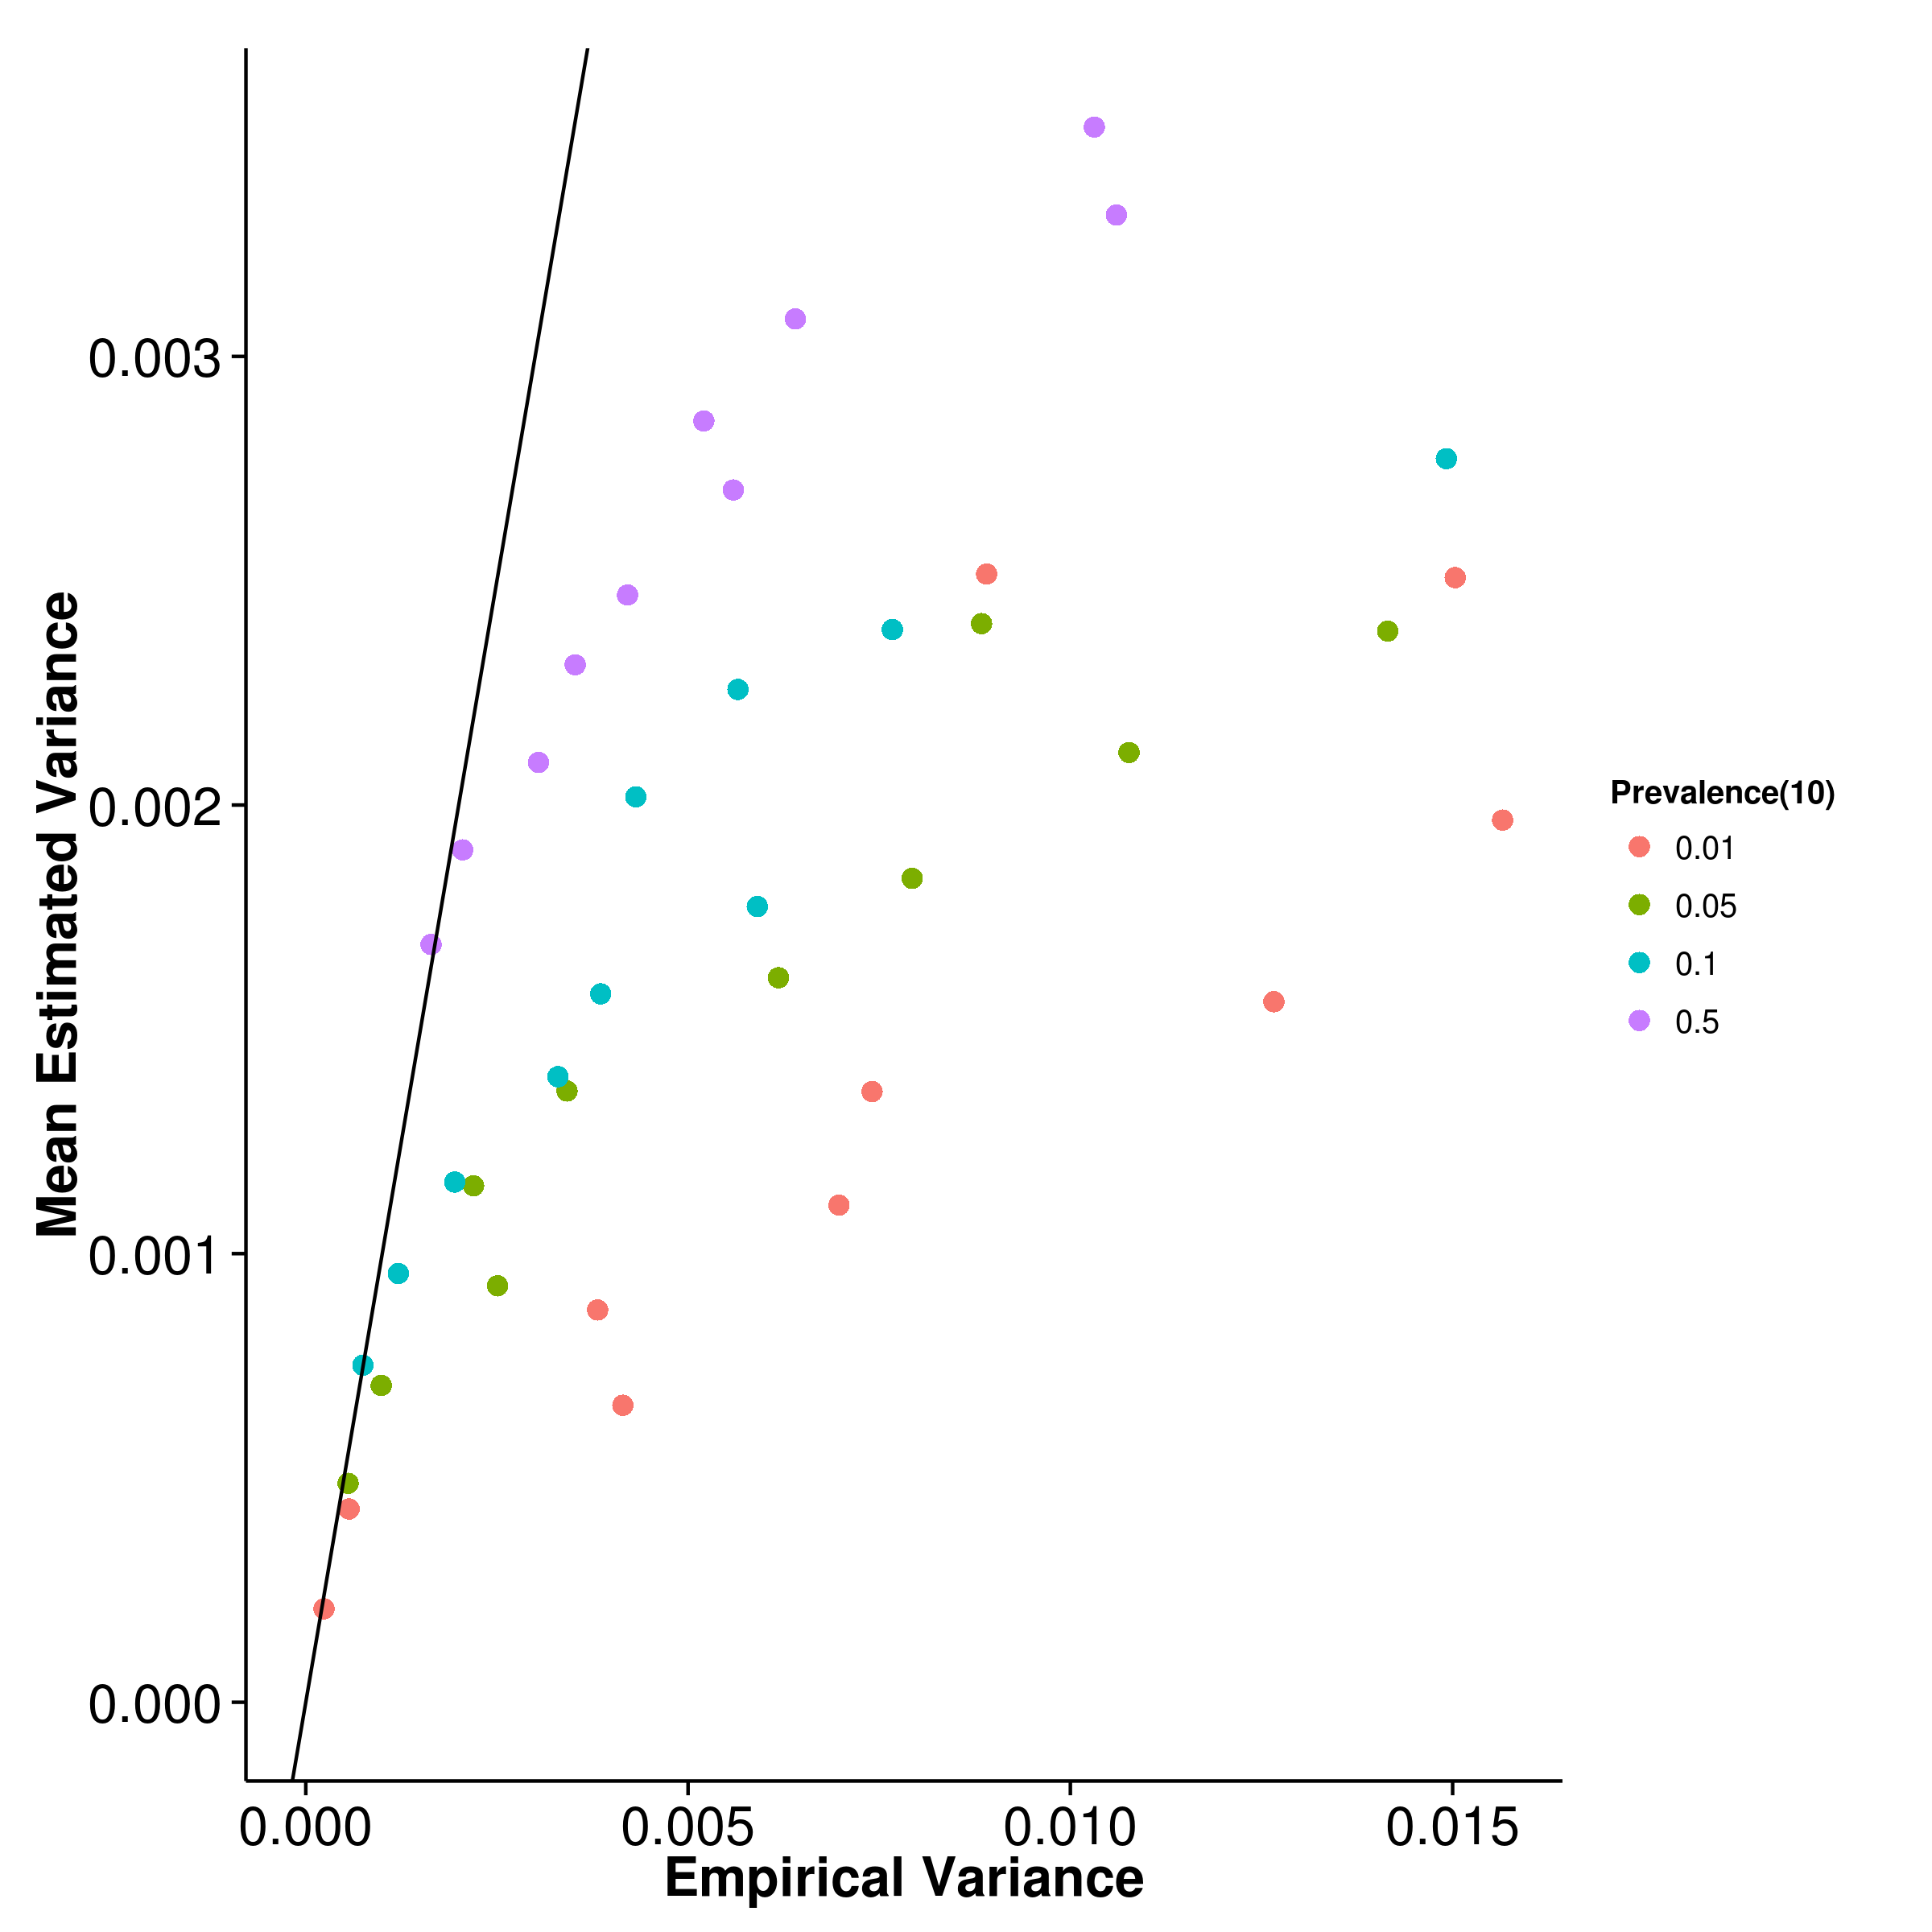
\includegraphics{figure/he_summary/cc_10c/shrek_CC_Rand_sdCom.png}}
					\label{fig:shrekCC10RandVarCom}
				}
				\subfloat[GCTA]{
					\scalebox{.4}{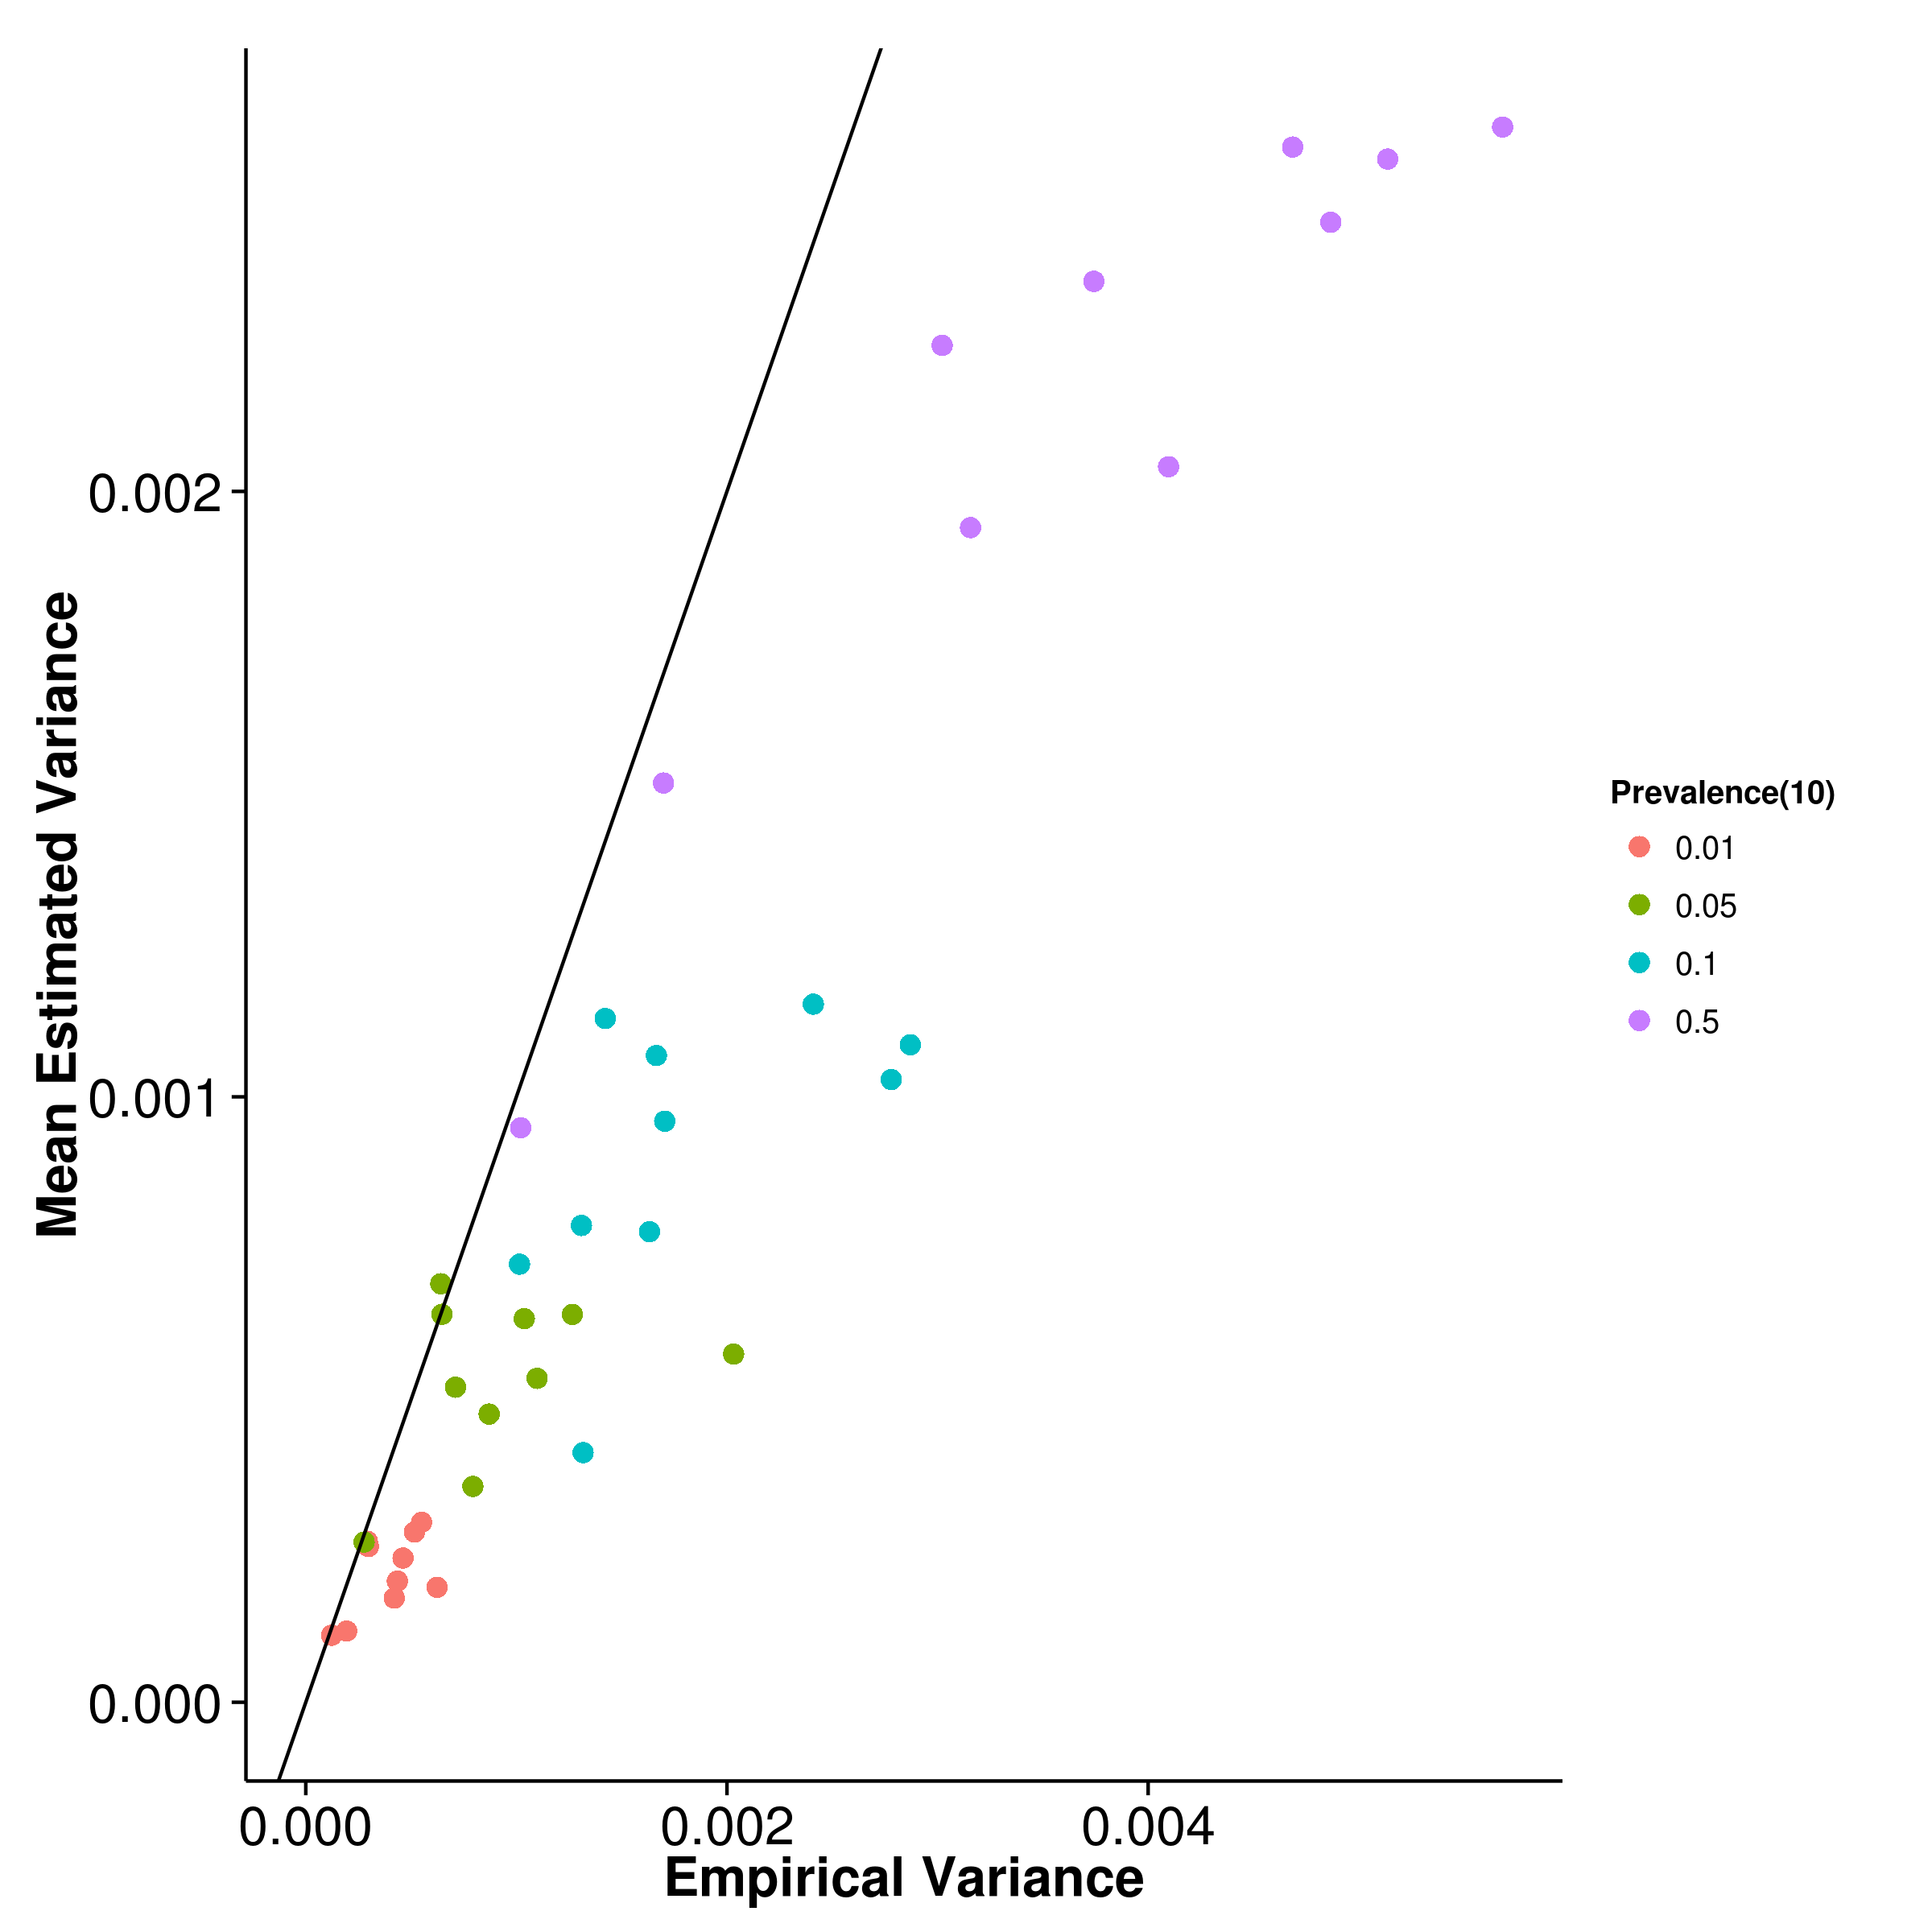
\includegraphics{figure/he_summary/cc_10c/gcta_CC_Rand_sdCom.png}}
					\label{fig:gctaCC10RandVarCom}
				}\\
				\subfloat[LDSC with fix intercept]{
					\scalebox{.4}{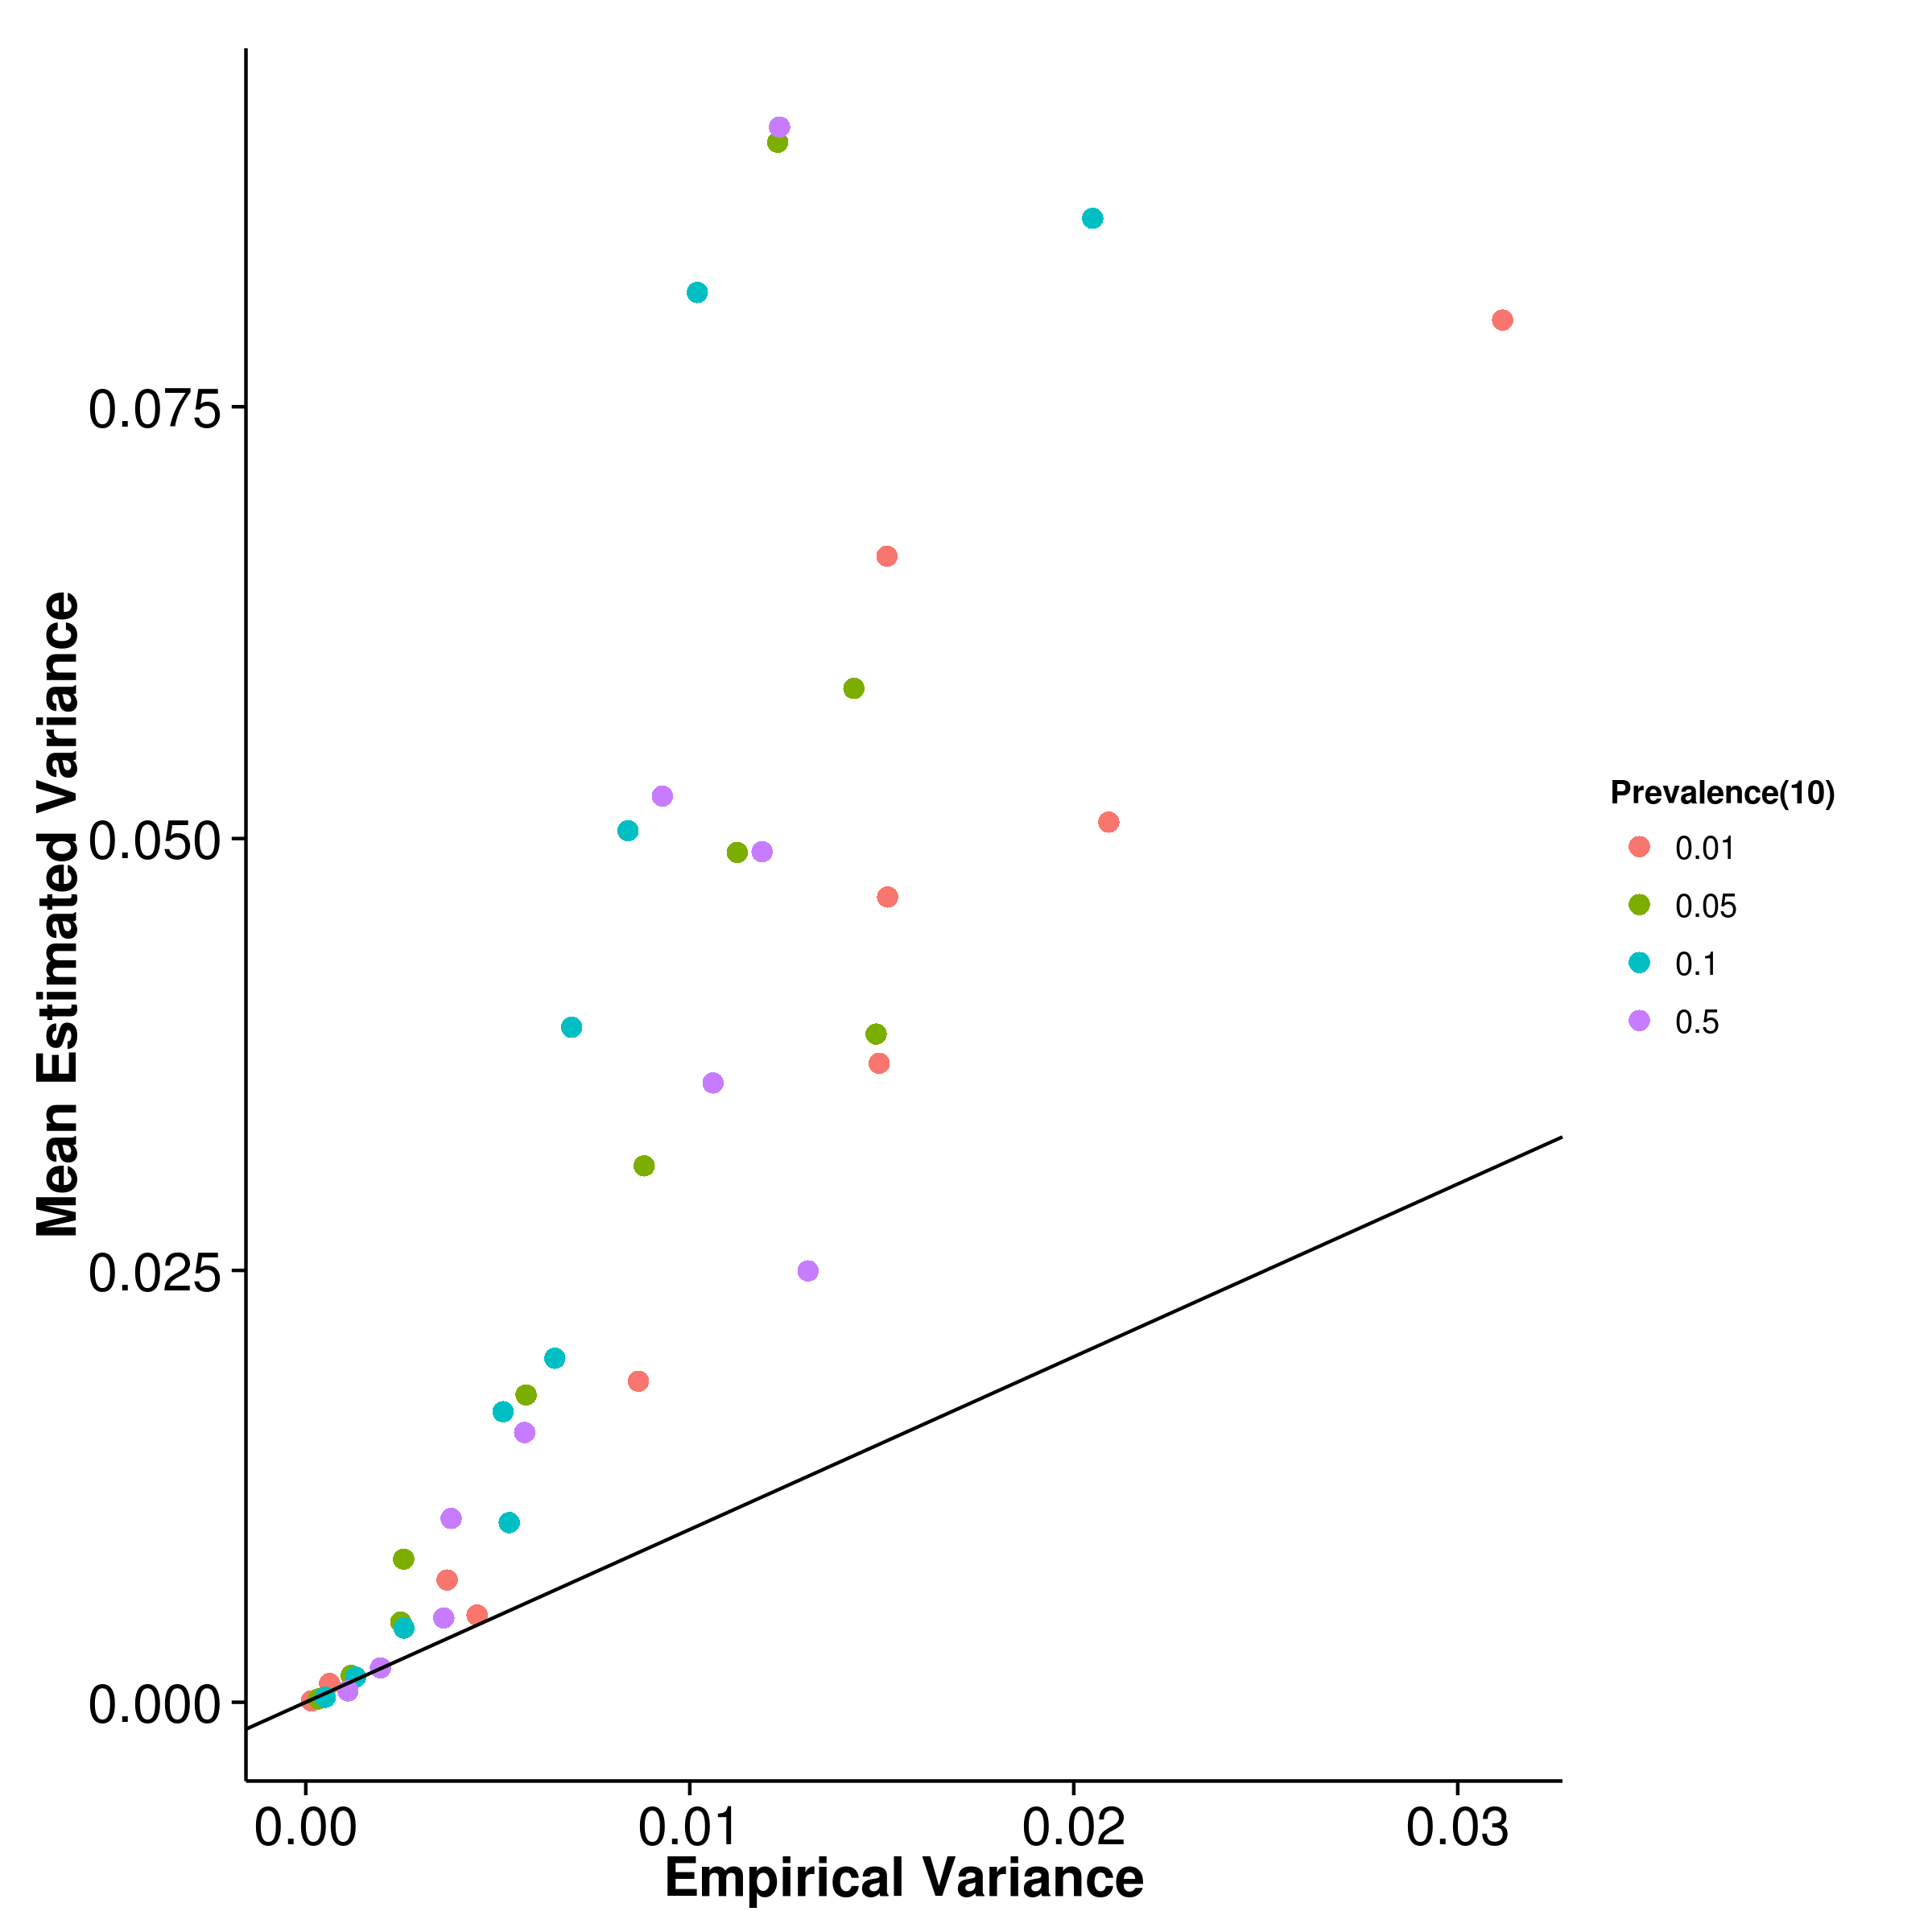
\includegraphics{figure/he_summary/cc_10c/ldsc_CC_Rand_sdCom.png}}
					\label{fig:ldscCC10RandVarCom}
				}
				\subfloat[LDSC with intercept estimation]{
					
					\scalebox{.4}{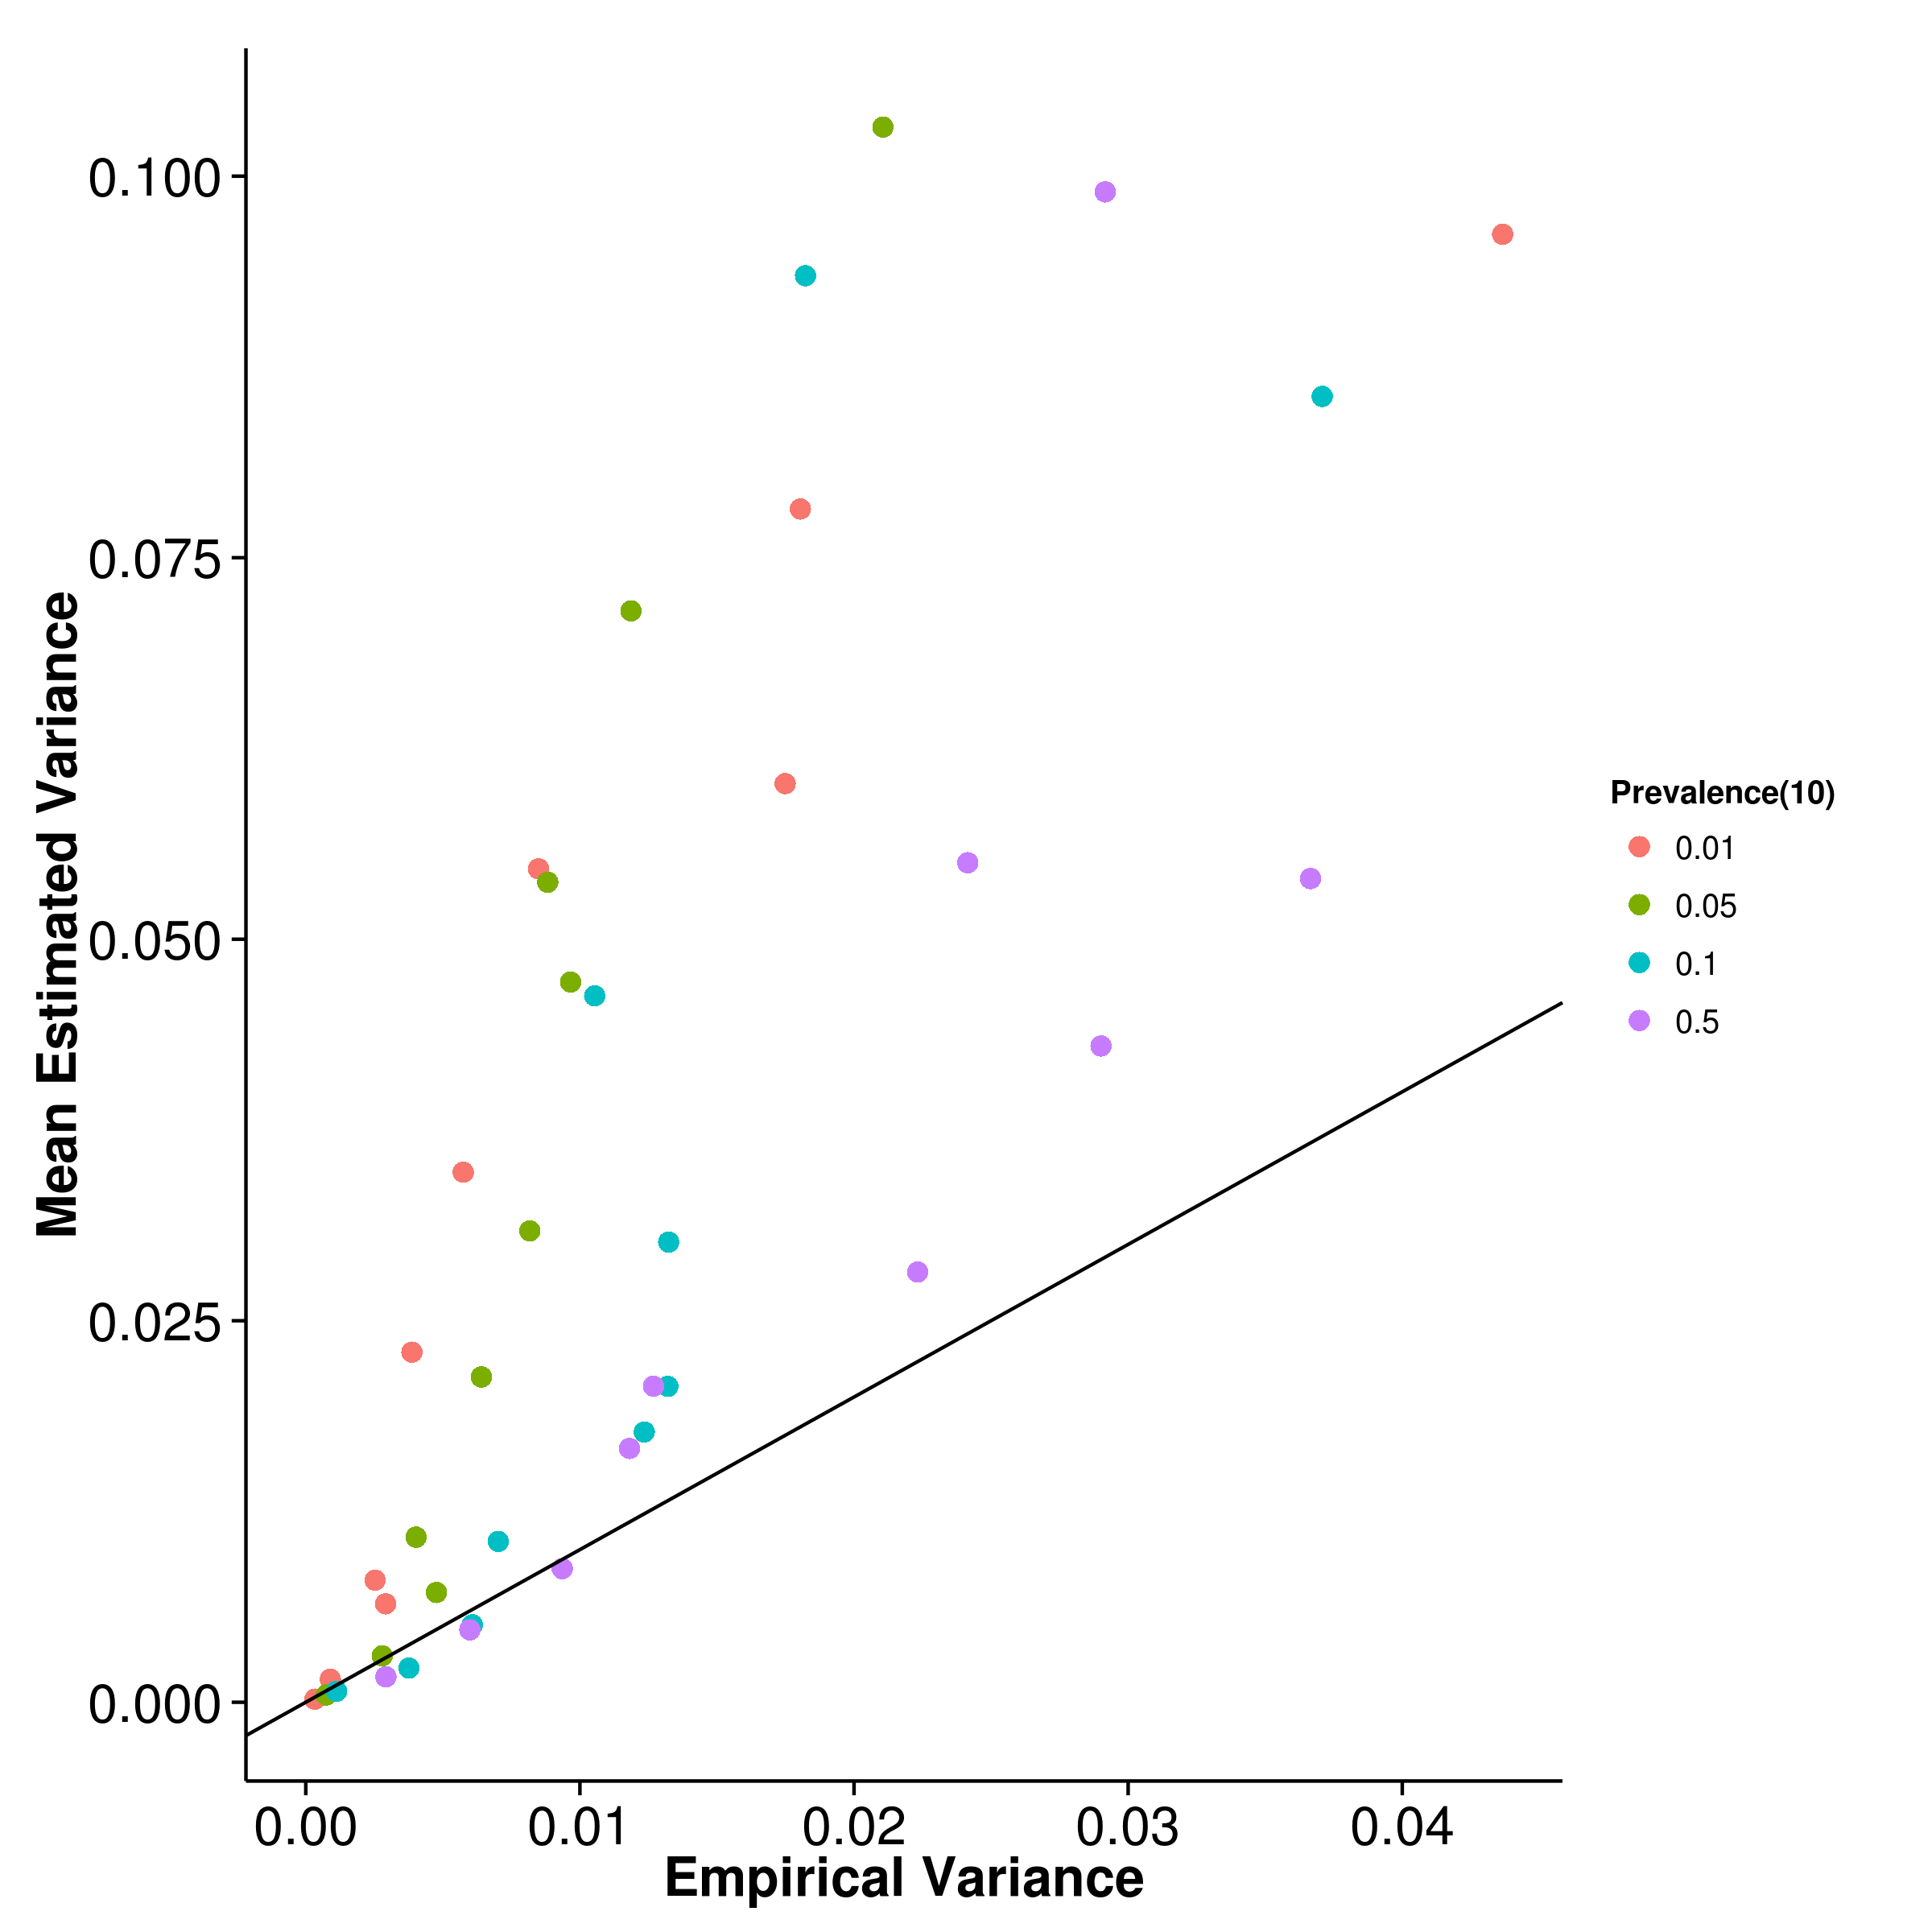
\includegraphics{figure/he_summary/cc_10c/ldscIn_CC_Rand_sdCom.png}}
					\label{fig:ldscInCC10RandVarCom}
				}
				\caption[Estimation of Variance in Case Control Simulation (10 Causal)]
				{Estimated variance of results from case control simulation with random effect size simulation when compared to empirical variance when 10 causal \glspl{SNP} was simulated.
					A general underestimation was observed for \gls{shrek} and \gls{gcta} whereas a larger upward bias was observed for \gls{ldsc}.} 
				\label{fig:CC10RandVarCom}
			\end{figure}
			
		In order to estimate the heritability from case control studies, it is important to model the disease status under a liability threshold model, which require knowledge of the population prevalence of the disease.
		Given that both the population prevalence and trait heritability can have a large influence to the performance of \gls{SNP} heritability estimation, simulations were performed where the population prevalence, the trait heritability and the number of causal \glspl{SNP} were varied. 
		
		When only 10 causal \glspl{SNP} were simulated, it is clear that the population prevalence has a significant impact to the performance of the algorithms (\cref{fig:CC10RandMean}). 
		Of all the algorithms tested, \gls{gcta} is the most affected by the population prevalence (\cref{fig:gctaCC10RandMean}), where the estimates from \gls{gcta} are generally underestimated.
		As the population prevalence decreases, the magnitude of bias increases, as reported by \citet{Golan2014}.
		On the other hand, the estimates generated by \gls{ldsc} with fixed intercept and \gls{shrek} are upwardly biased.
		The magnitude of bias also increases as the population prevalence decreases.
		Surprisingly, when intercept estimation was performed, a downward bias is observed in the estimates from \gls{ldsc}.
		The magnitude of bias is also relatively smaller when compared to \gls{ldsc} with fixed intercept.
		The same pattern are observed when different number of causal \glspl{SNP} were simulated (\cref{fig:CC50RandMean,fig:CCRandMean,fig:CC500RandMean}).
		
		Of all the algorithms, \gls{gcta} has the smallest average empirical variance (\cref{fig:gctaCC10RandVar}) where \gls{ldsc} with intercept estimation has the largest empirical variance.
		On the other hand, it is observed that the estimates from \gls{shrek} (\cref{fig:shrekCC10RandVar}) and \gls{ldsc} (\cref{fig:ldscCC10RandVar}) with fixed intercept have similar empirical variance.
		As the number of causal \glspl{SNP} increases, the empirical variance of all algorithms  decreases (\cref{fig:CC50RandVar,fig:CCRandVar,fig:CC500RandVar}) similar to the results from the quantitative trait simulation.
		
		It is observed that \gls{shrek} consistently underestimate its empirical variance where the magnitude of bias increases as population prevalence decreases  (\cref{fig:shrekCC10RandVarCom}).
		On the other hand, \gls{gcta} can provide a more accurate estimation for its empirical variance, only moderately underestimated the variance  (\cref{fig:gctaCC10RandVarCom}).
		Again, it is observed that \gls{ldsc} consistently overestimate its empirical variance (\cref{fig:CC10RandVarCom}). 
		However, as the number of causal \glspl{SNP} increases, the magnitude of bias observed in the estimation of variance decreases for \gls{ldsc} (\cref{fig:CC50RandVarCom,fig:CCRandVarCom,fig:CC500RandVarCom}). 
		When 500 causal \glspl{SNP} were simulated, \gls{ldsc} can provide a relatively accurate estimates of its empirical variance (\cref{fig:ldscCC500RandVarCom}).
		
		Overall, \gls{shrek} has the best average performance of all the algorithm tested (\cref{tab:mseCC}).
		Interestingly, although no confounding factors were simulated, it is observed that \gls{ldsc} with intercept estimation has a better performance than \gls{ldsc} with fixed intercept when the prevalence is small.
		Therefore, it is possible for the intercept estimation to help correcting for some of bias introduced by case control sampling.
		
\begin{table}
	\centering
	\begin{tabular}{p{2cm}p{2.4cm}rrrr}
		\toprule
		Population Prevalence&	Number of Causal SNPs&	SHREK&	LDSC&	LDSC-In&	GCTA \\
		\midrule
		0.01&	10&	\textbf{0.0145}&	0.0361&	0.0164&	0.0675\\
		0.01&	50&	0.0135&	0.0254&	\textbf{0.00791}&	0.0702\\
		0.01&	100&	0.0128&	0.0227&	\textbf{0.0102}&	0.0698\\
		0.01&	500&	\textbf{0.0126}&	0.0214&	0.0150&	0.0710\\
		0.05&	10&	0.0110&	0.0201&	\textbf{0.00983}&	0.0302\\
		0.05&	50&	\textbf{0.00453}&	0.00974&	0.0115&	0.0299\\
		0.05&	100&	\textbf{0.00569}&	0.0113&	0.00981&	0.0304\\
		0.05&	500&	\textbf{0.00540}&	0.00999&	0.0171&	0.0305\\
		0.1&	10&	\textbf{0.00512}&	0.0109&	0.0301&	0.0165\\
		0.1&	50&	\textbf{0.00381}&	0.00824&	0.0105&	0.0152\\
		0.1&	100&	\textbf{0.00418}&	0.00802&	0.0163&	0.0148\\
		0.1&	500&	\textbf{0.00400}&	0.00740&	0.0141&	0.0155\\
		0.5&	10&	0.00560&	0.00749&	0.0219&	\textbf{0.00410}\\
		0.5&	50&	0.00362&	0.00528&	0.0232&	\textbf{0.00244}\\
		0.5&	100&	0.00356&	0.00460&	0.0208&	\textbf{0.00225}\\
		0.5&	500&	0.00338&	0.00365&	0.0159&	\textbf{0.00200}\\
		\bottomrule
	\end{tabular}
	\caption[MSE of Case Control Simulation]{
		\Gls{mse} of Case Control simulation.
		Algorithm with the best performance under each condition were \textbf{bold-ed}.
		Of all the algorithms, \gls{shrek} has the best average performance.
		It is observed that as the number of causal \glspl{SNP} increases, the \gls{mse} tends to decrease for all algorithms, similar to the results from quantitative trait simulation.
	}
	\label{tab:mseCC}
\end{table}

		Finally, when compared to the quantitative trait simulation, a smaller number of \glspl{SNP} and larger sample size (2,000 samples with 1,000 cases and 1,000 controls) were simulated. 
		Thus, the results from case control simulations are not directly comparable to the results from the quantitative trait simulations.
		
		\subsubsection{Extreme Phenotype Simulation}
			%Mean
			\begin{figure}
				\centering
				\subfloat[SHREK]{
					\scalebox{.4}{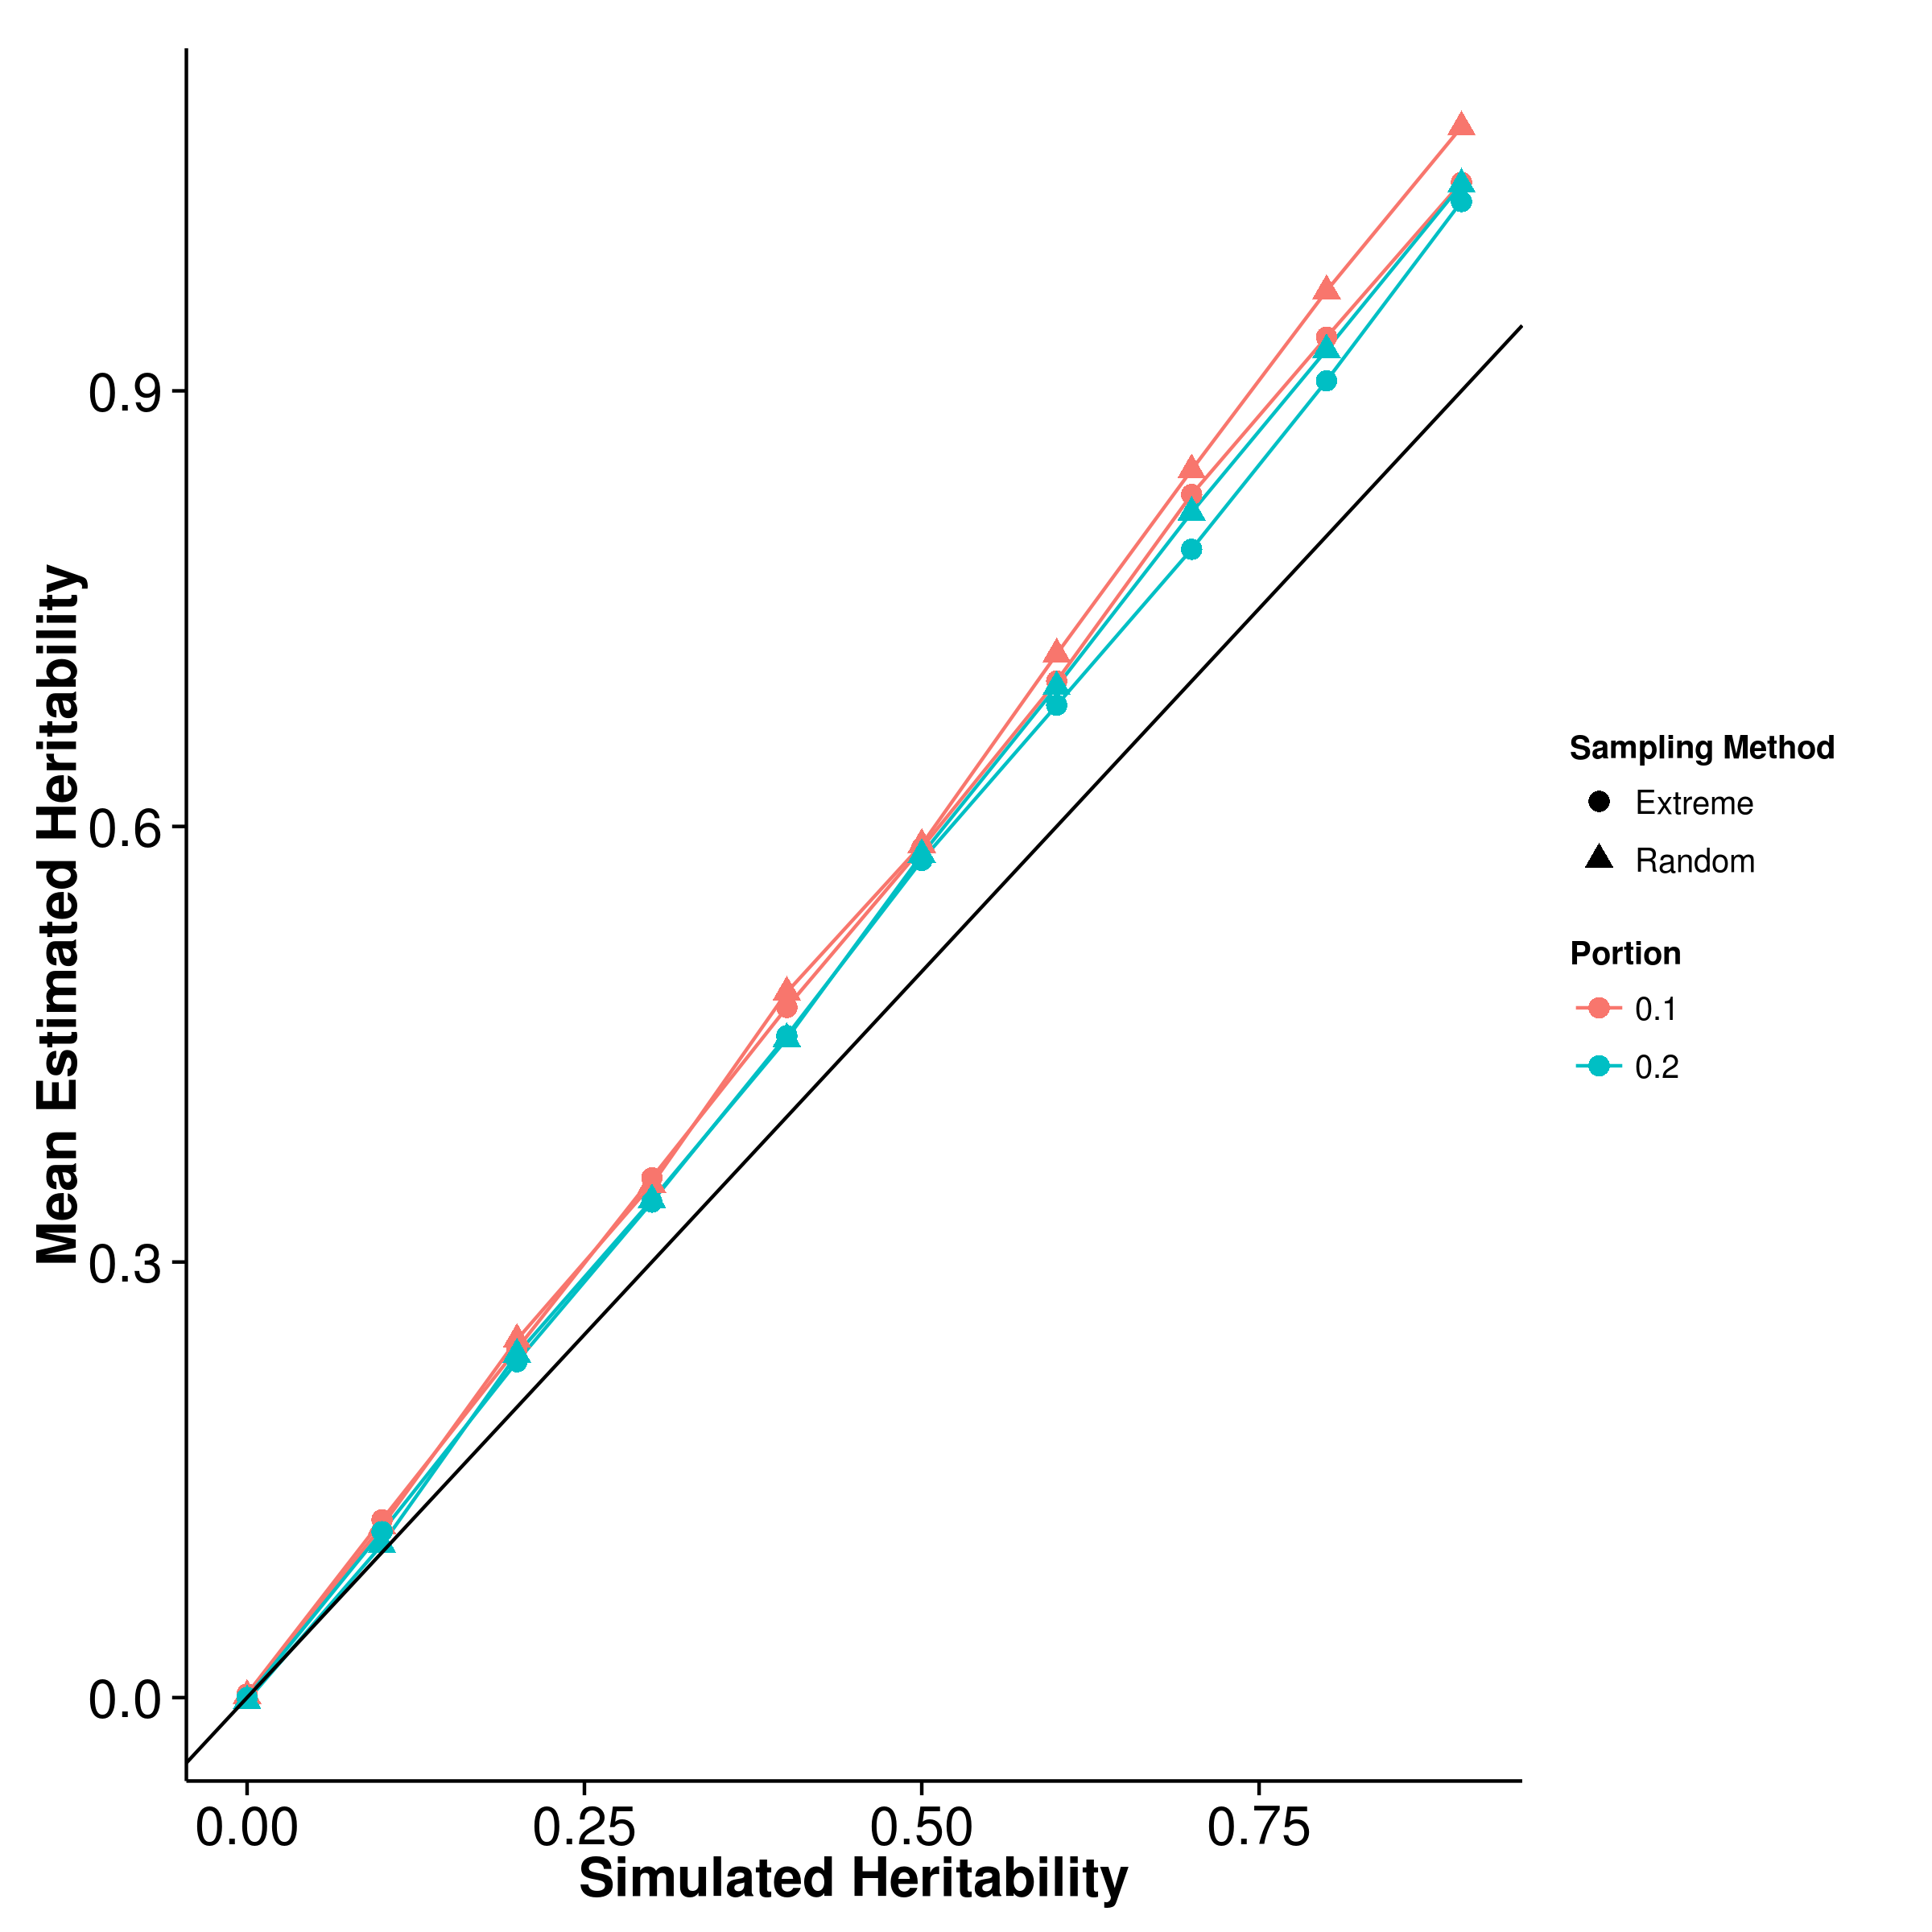
\includegraphics{figure/he_summary/pheno_extreme/shrek_extremeSelect_mean.png}}
					\label{fig:shrekExMean}
				}
				\subfloat[GCTA]{
					\scalebox{.4}{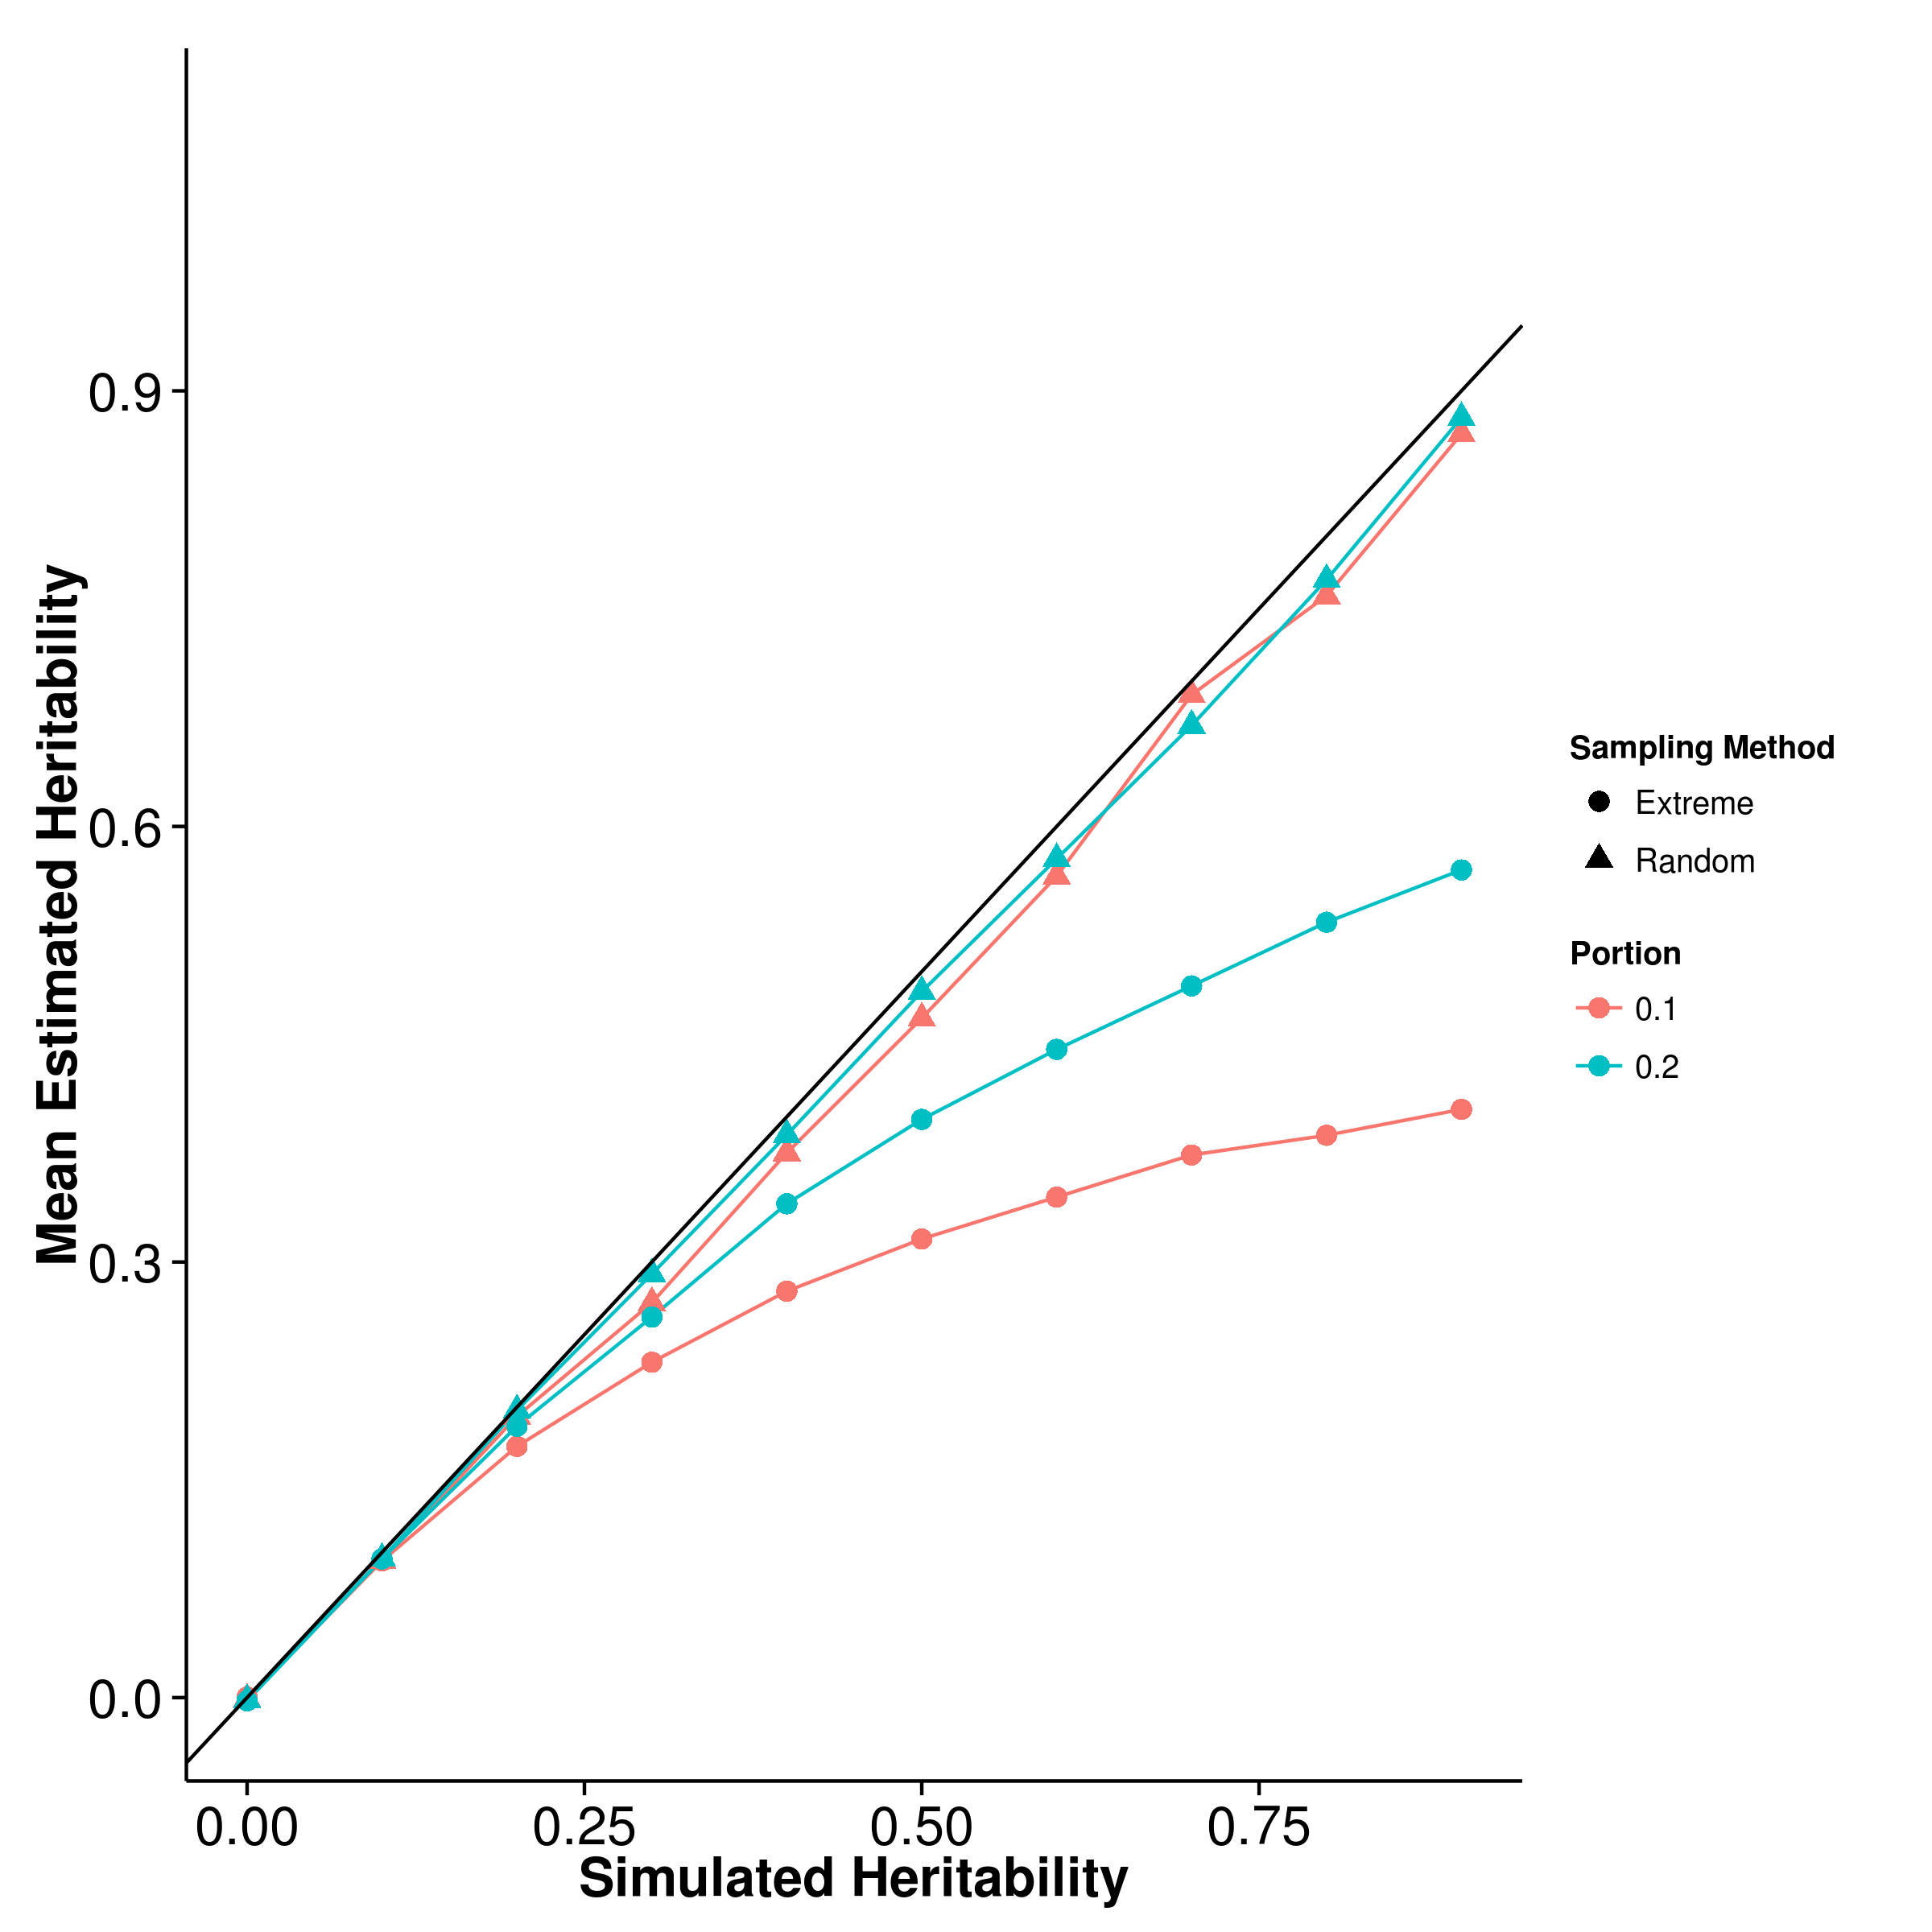
\includegraphics{figure/he_summary/pheno_extreme/gcta_extremeSelect_mean.png}}
					\label{fig:gctaExMean}
				}\\
				\subfloat[LDSC with fix intercept]{
					\scalebox{.4}{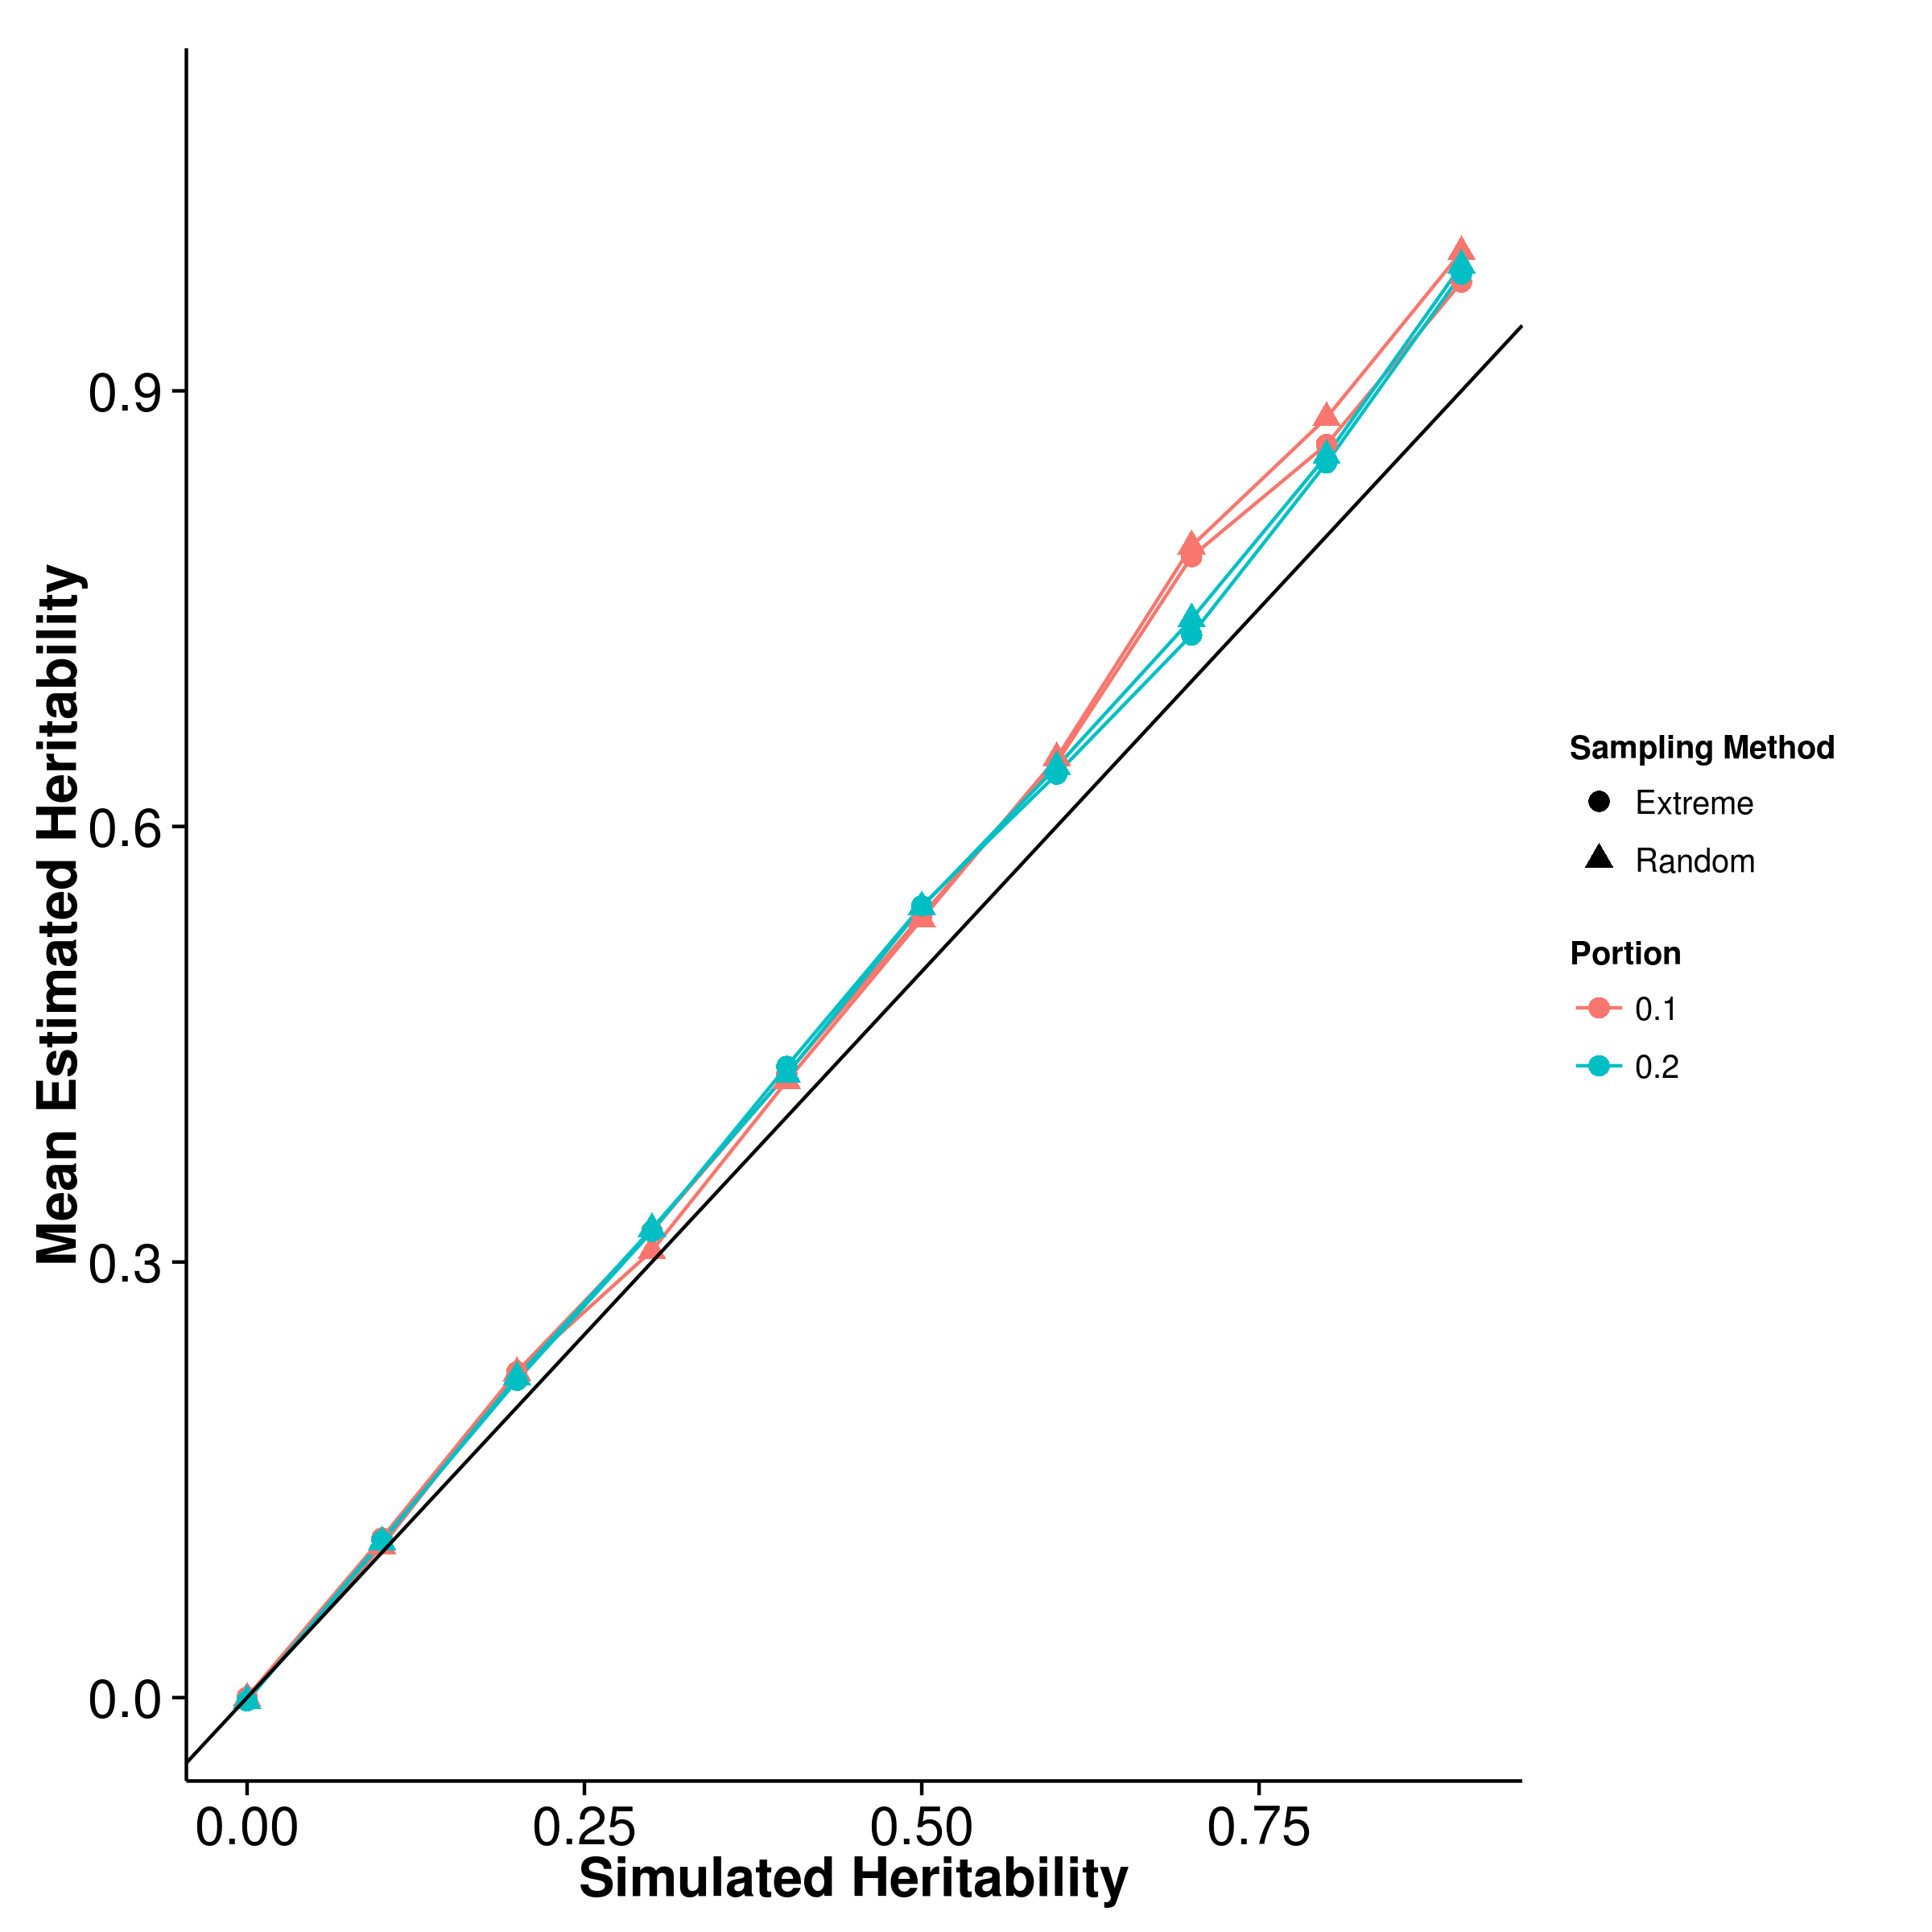
\includegraphics{figure/he_summary/pheno_extreme/ldsc_extremeSelect_mean.png}}
					\label{fig:ldscExMean}
				}
				\subfloat[LDSC with intercept estimation]{
					
					\scalebox{.4}{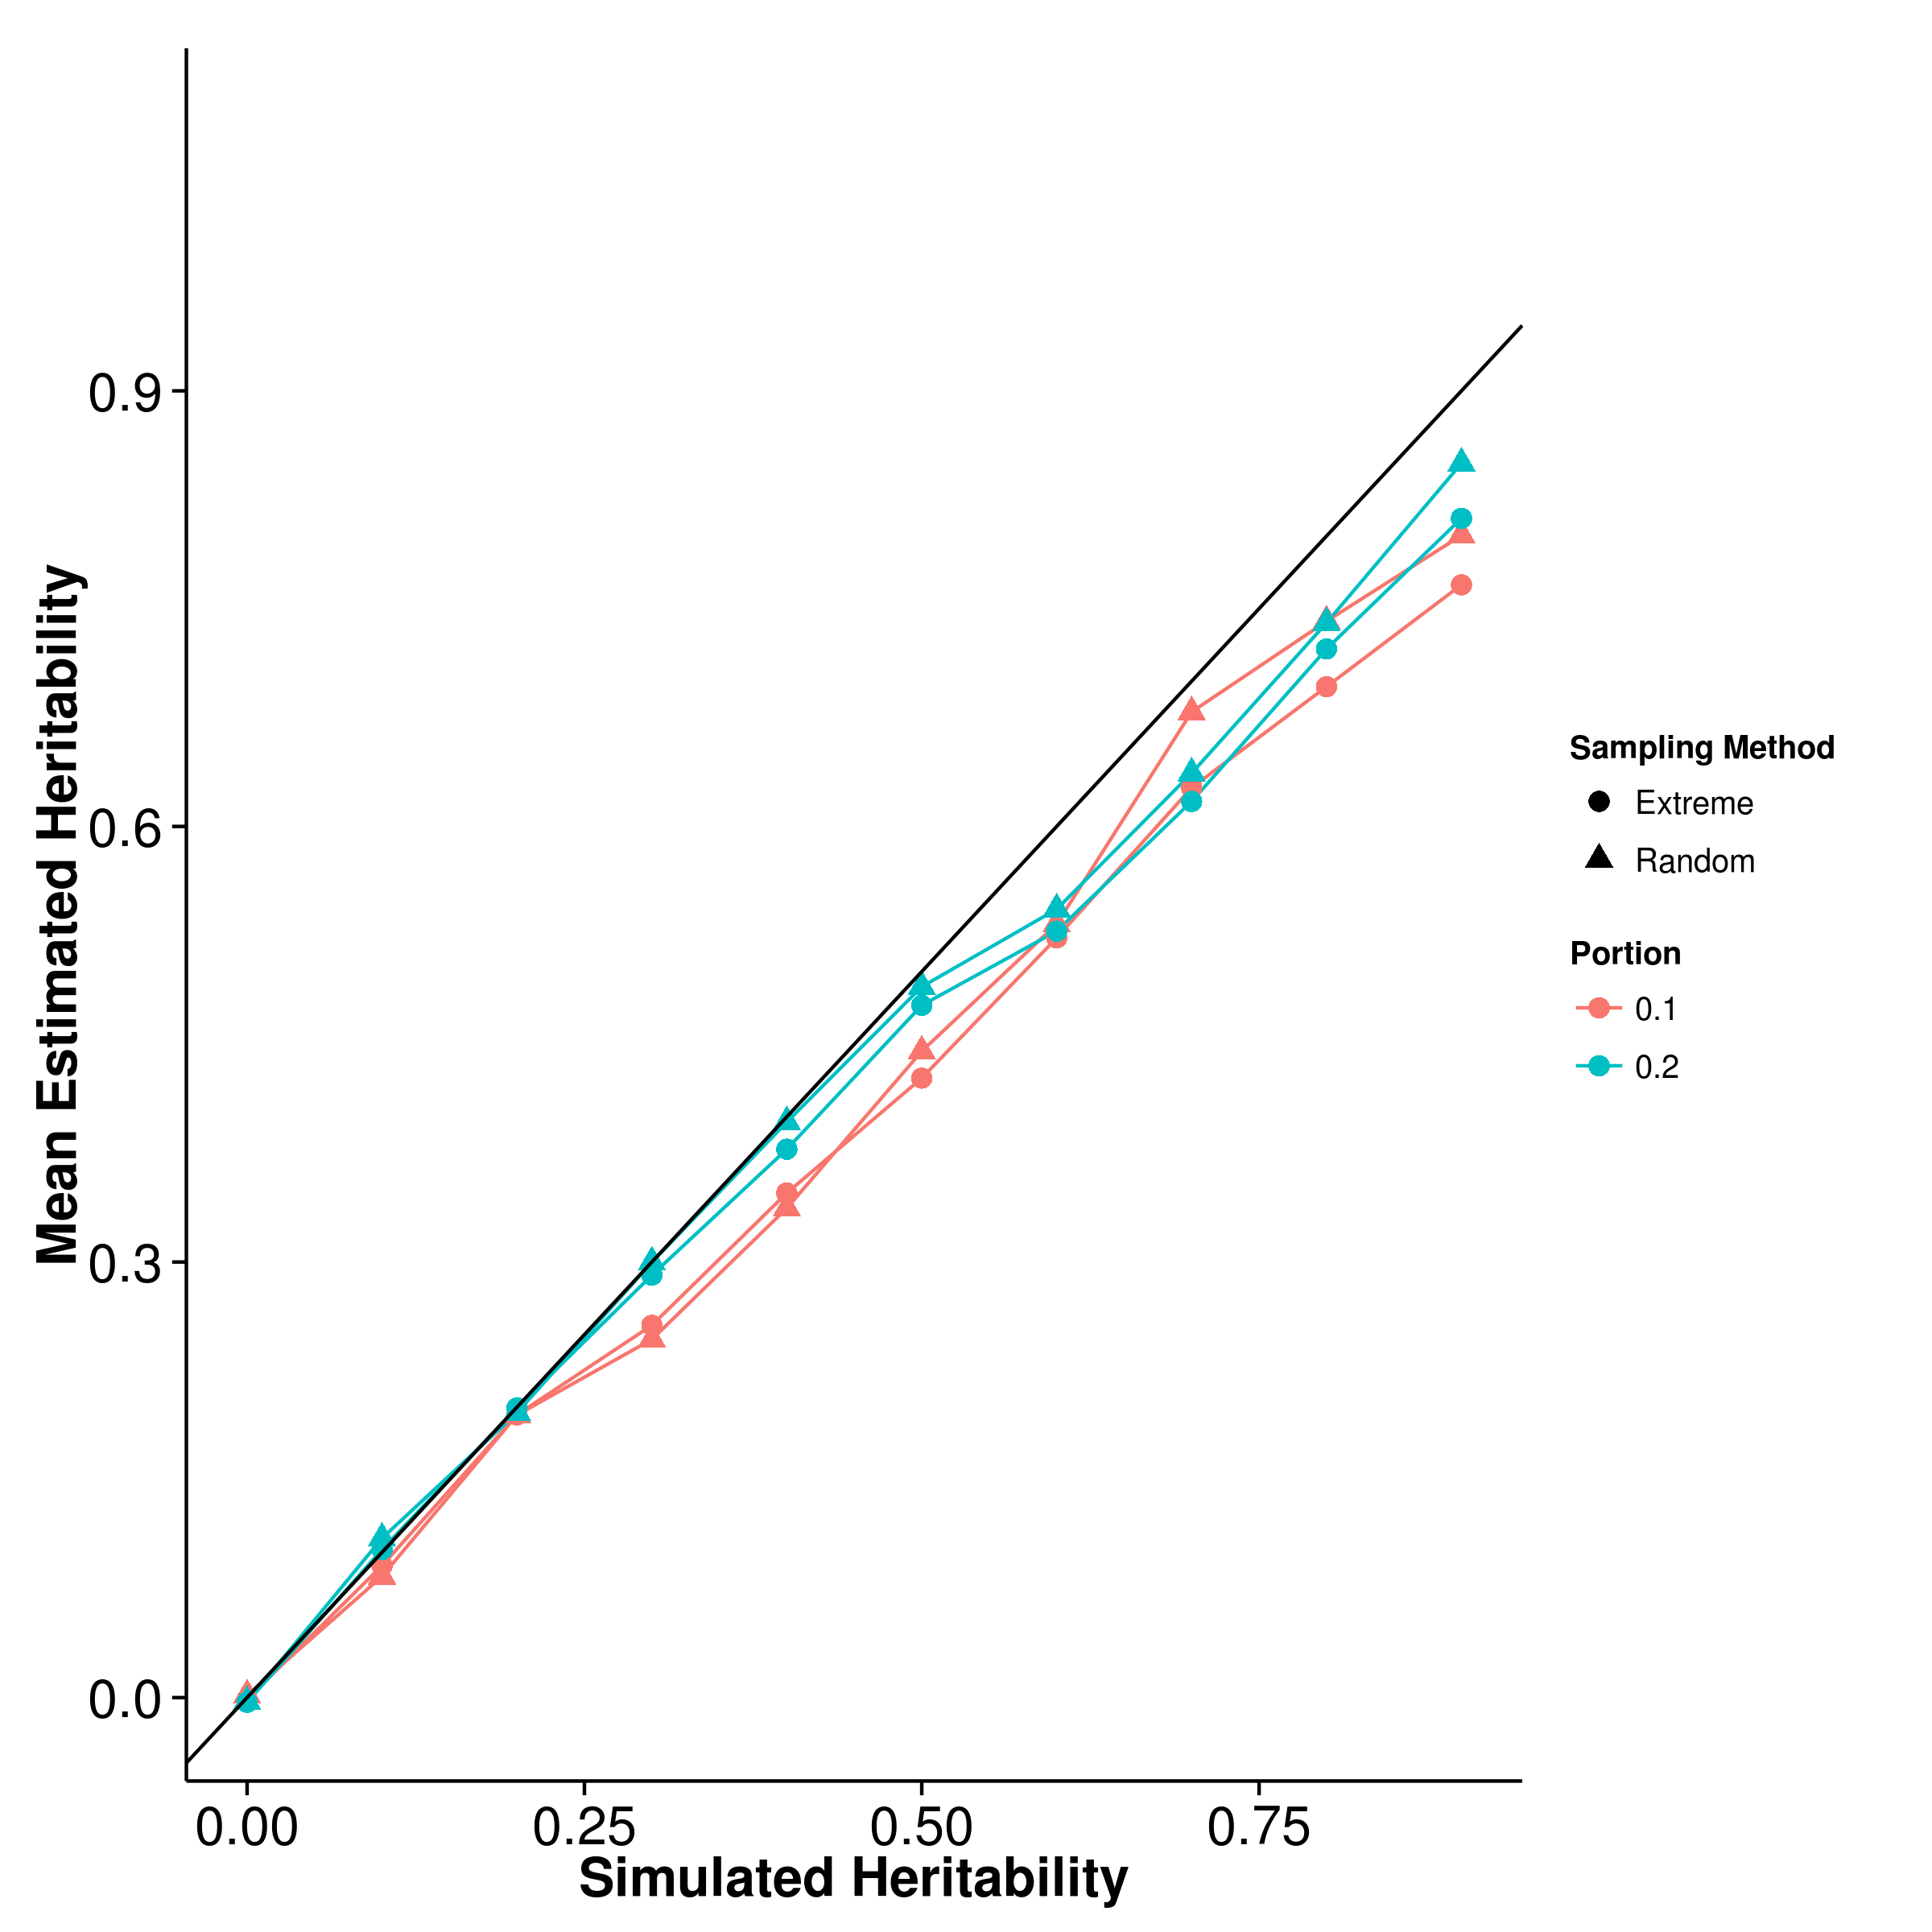
\includegraphics{figure/he_summary/pheno_extreme/ldscIn_extremeSelect_mean.png}}
					\label{fig:ldscInExMean}
				}
				\caption[Mean of Extreme Phenotype Selection Simulation Results]
				{Mean of results from extreme phenotype simulation.
					The performance of the algorithms when random sampling was performed were similar to what was observed in the quantitative trait simulation.
					However, when extreme phenotype was performed, a larger under estimation was observed for \gls{gcta} and it gets worst when the portion of sample selected decreases.
					On the other hand, the performance of \gls{shrek} and \gls{ldsc} under the extreme phenotype selection was similar to that from the random samplings.
				} 
				\label{fig:ExMean}
			\end{figure}
			%Empirical Variance
			\begin{figure}
				\centering
				\subfloat[SHREK]{
					\scalebox{.4}{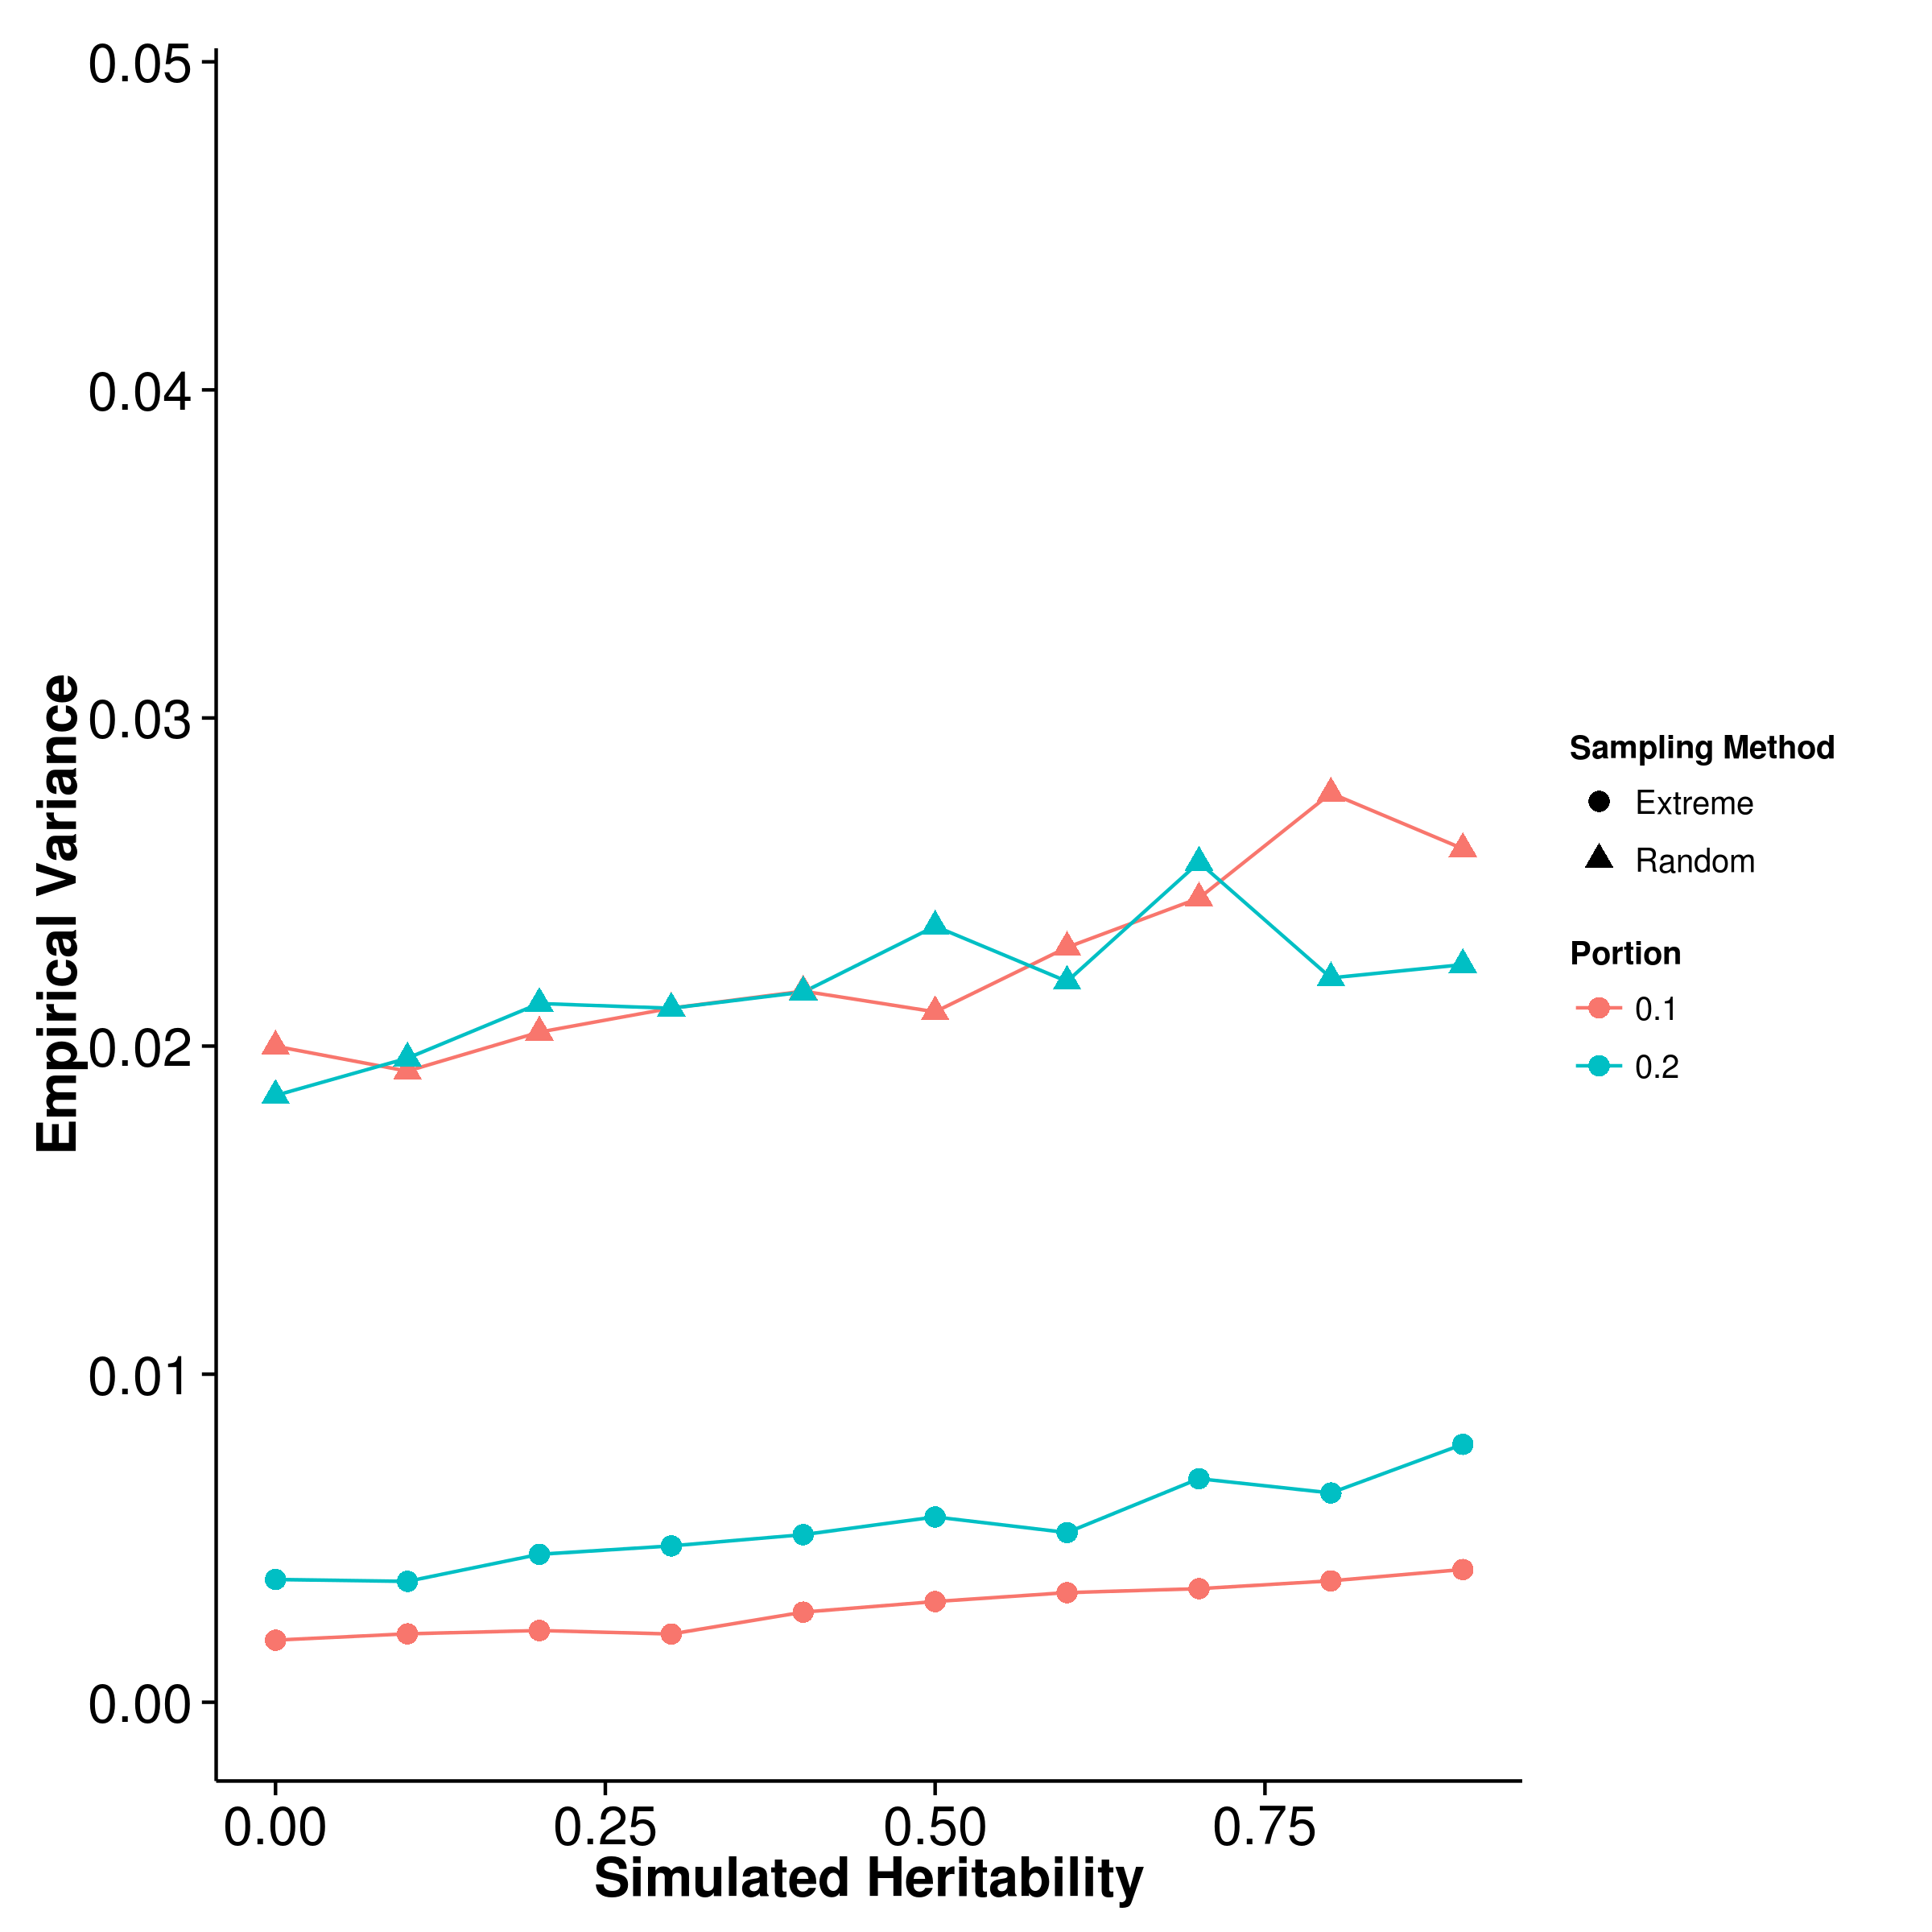
\includegraphics{figure/he_summary/pheno_extreme/shrek_extremeSelect_var.png}}
					\label{fig:shrekExVar}
				}
				\subfloat[GCTA]{
					\scalebox{.4}{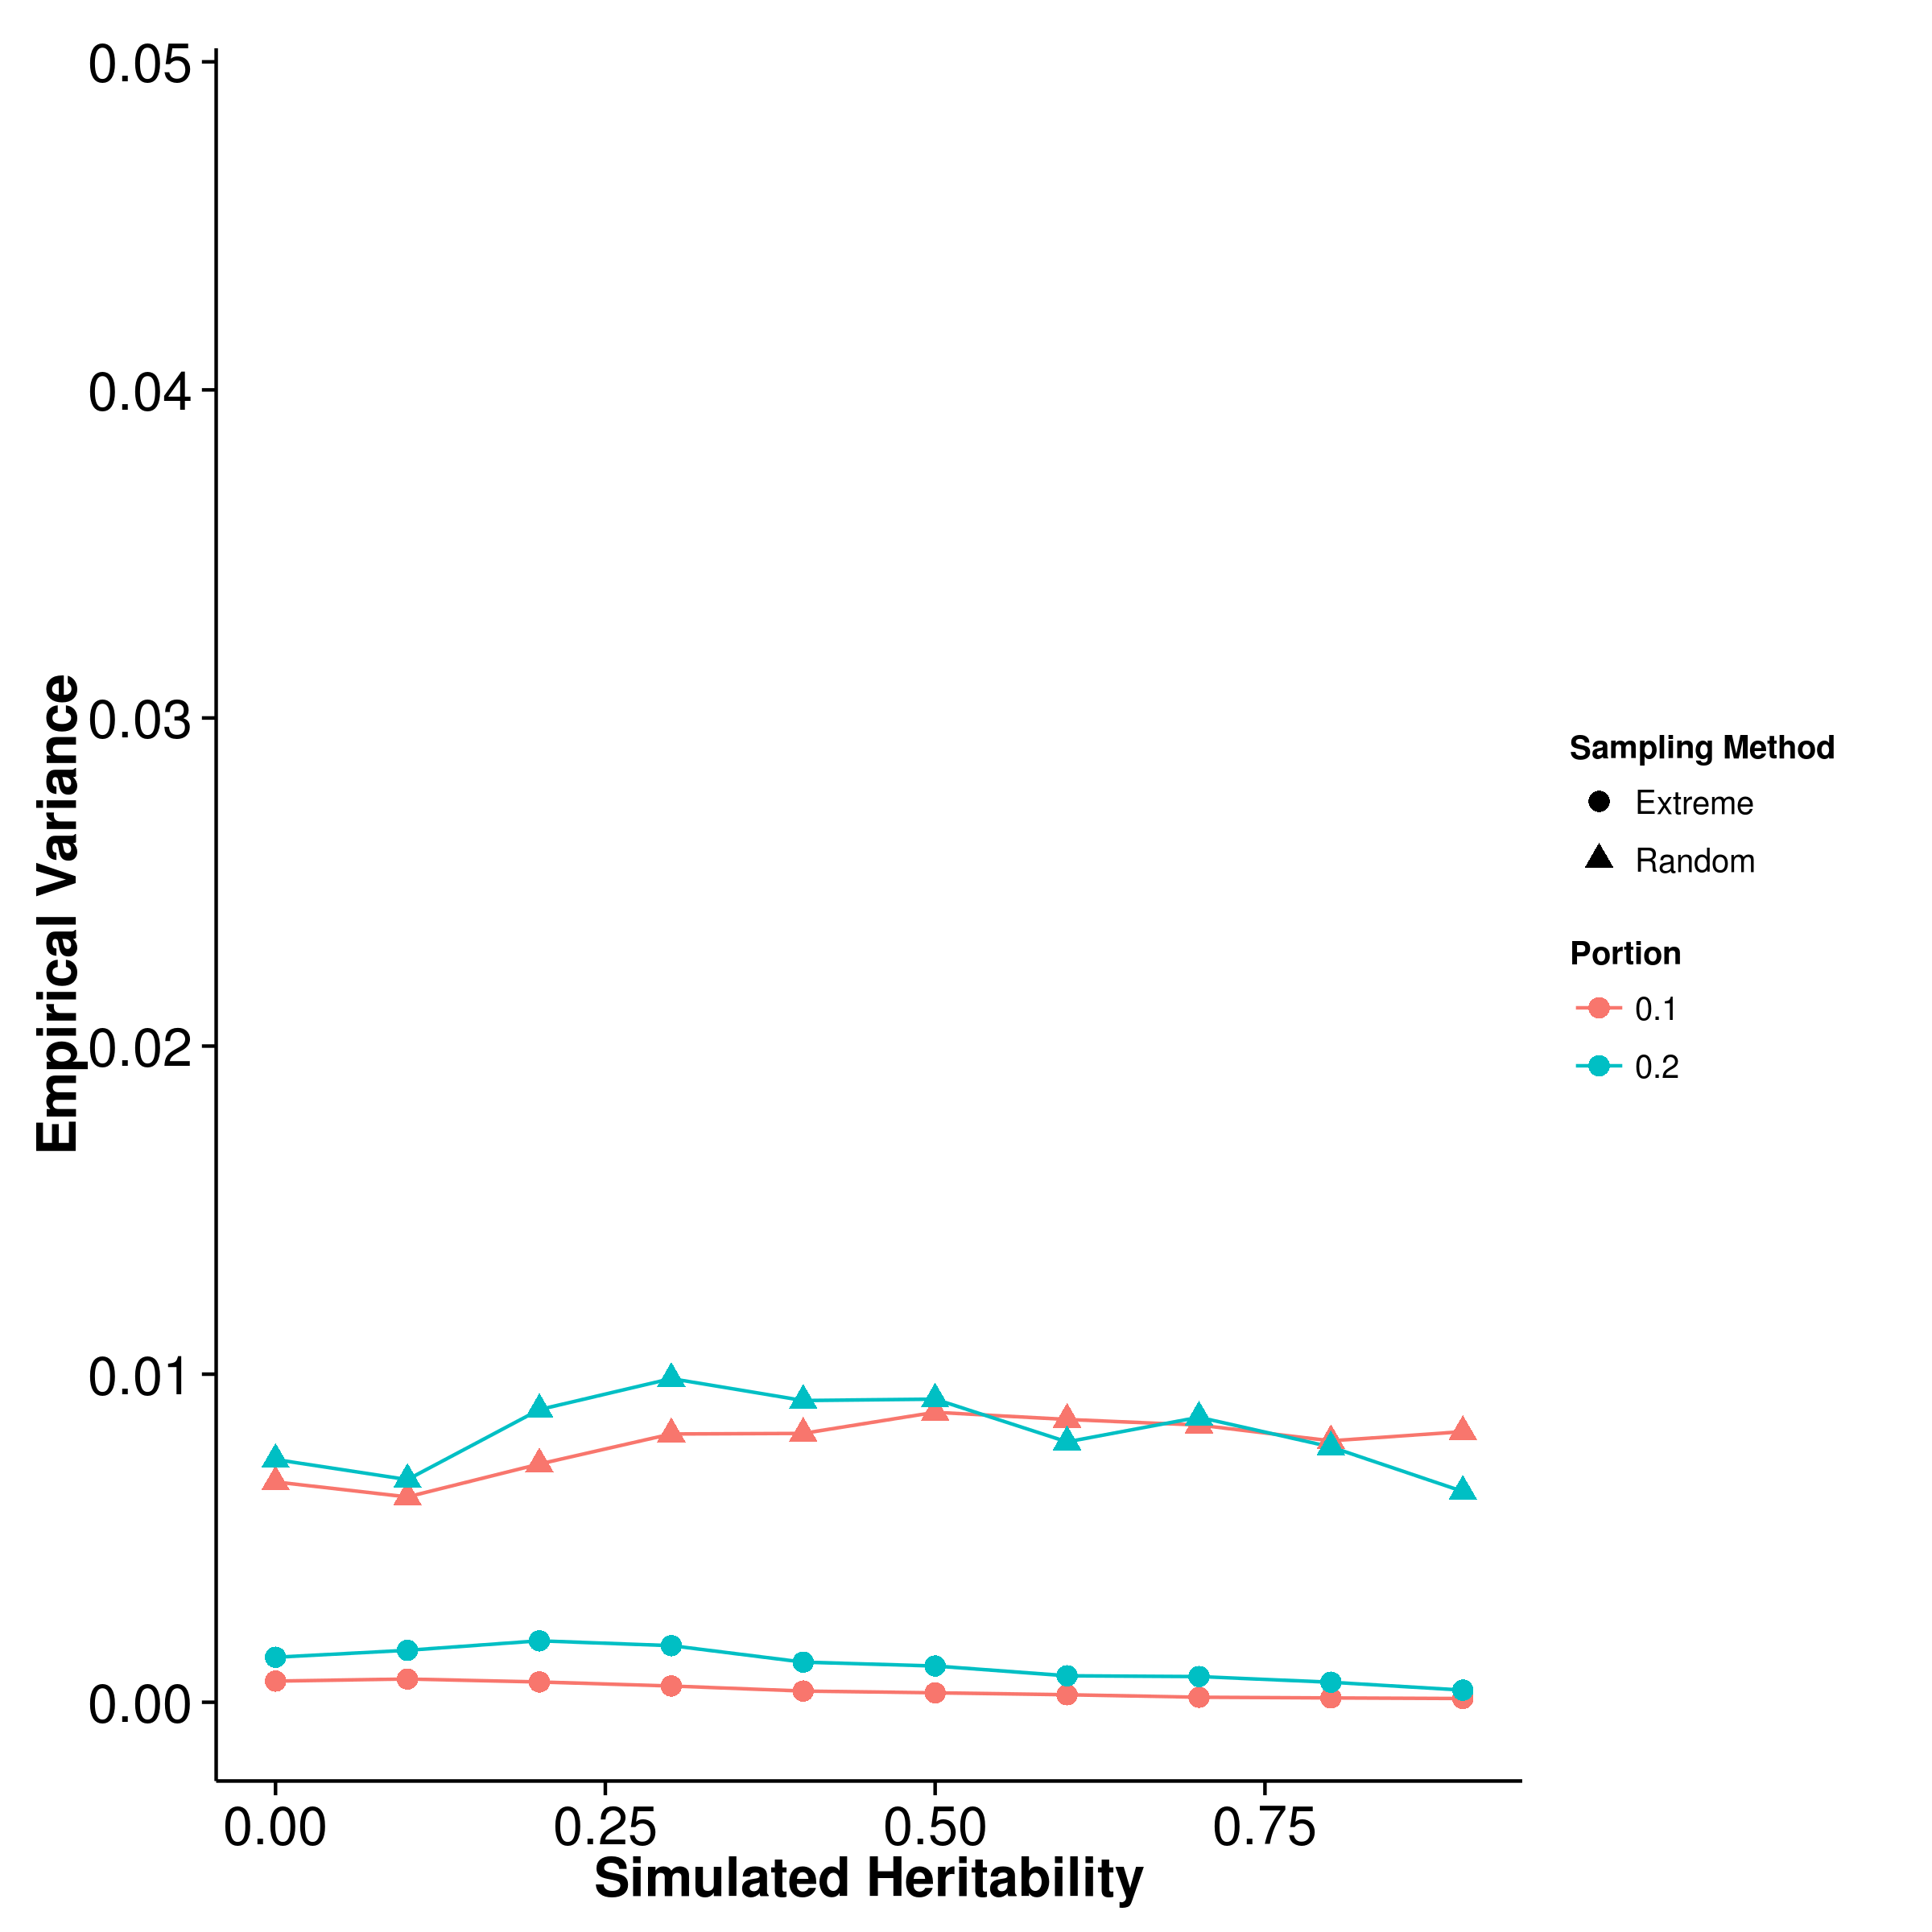
\includegraphics{figure/he_summary/pheno_extreme/gcta_extremeSelect_var.png}}
					\label{fig:gctaExVar}
				}\\
				\subfloat[LDSC with fix intercept]{
					\scalebox{.4}{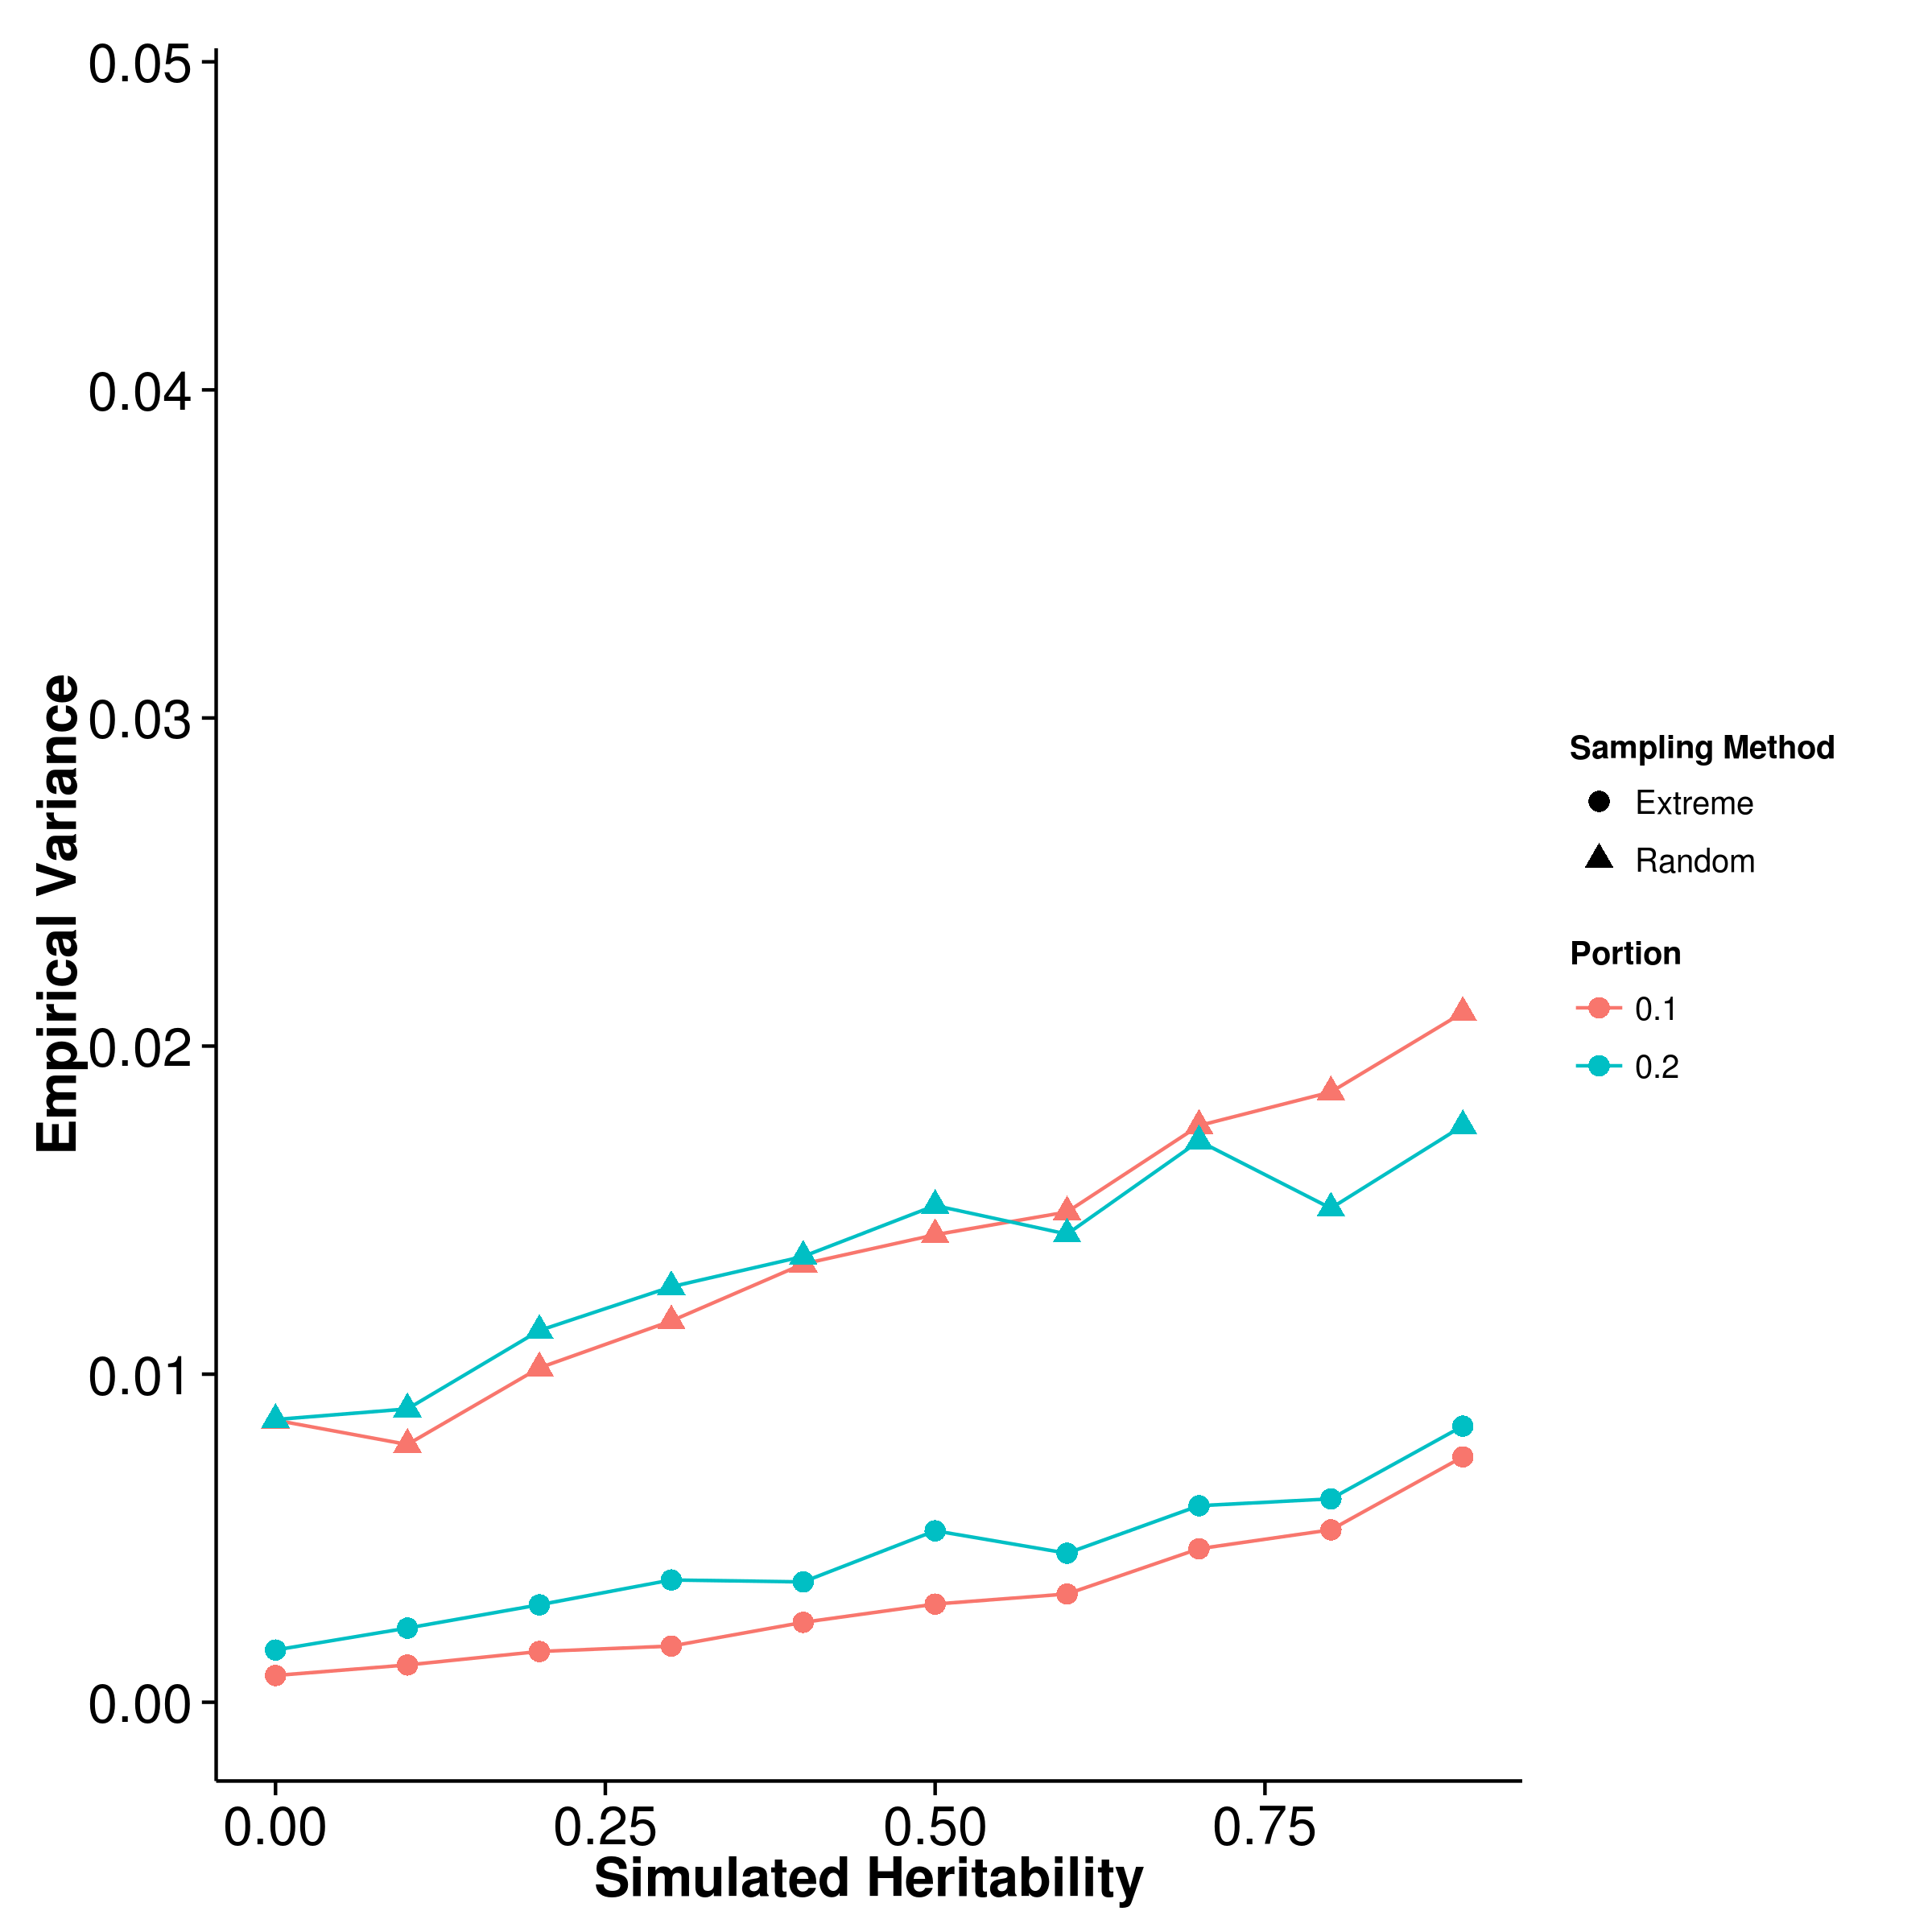
\includegraphics{figure/he_summary/pheno_extreme/ldsc_extremeSelect_var.png}}
					\label{fig:ldscEx}
				}
				\subfloat[LDSC with intercept estimation]{
					
					\scalebox{.4}{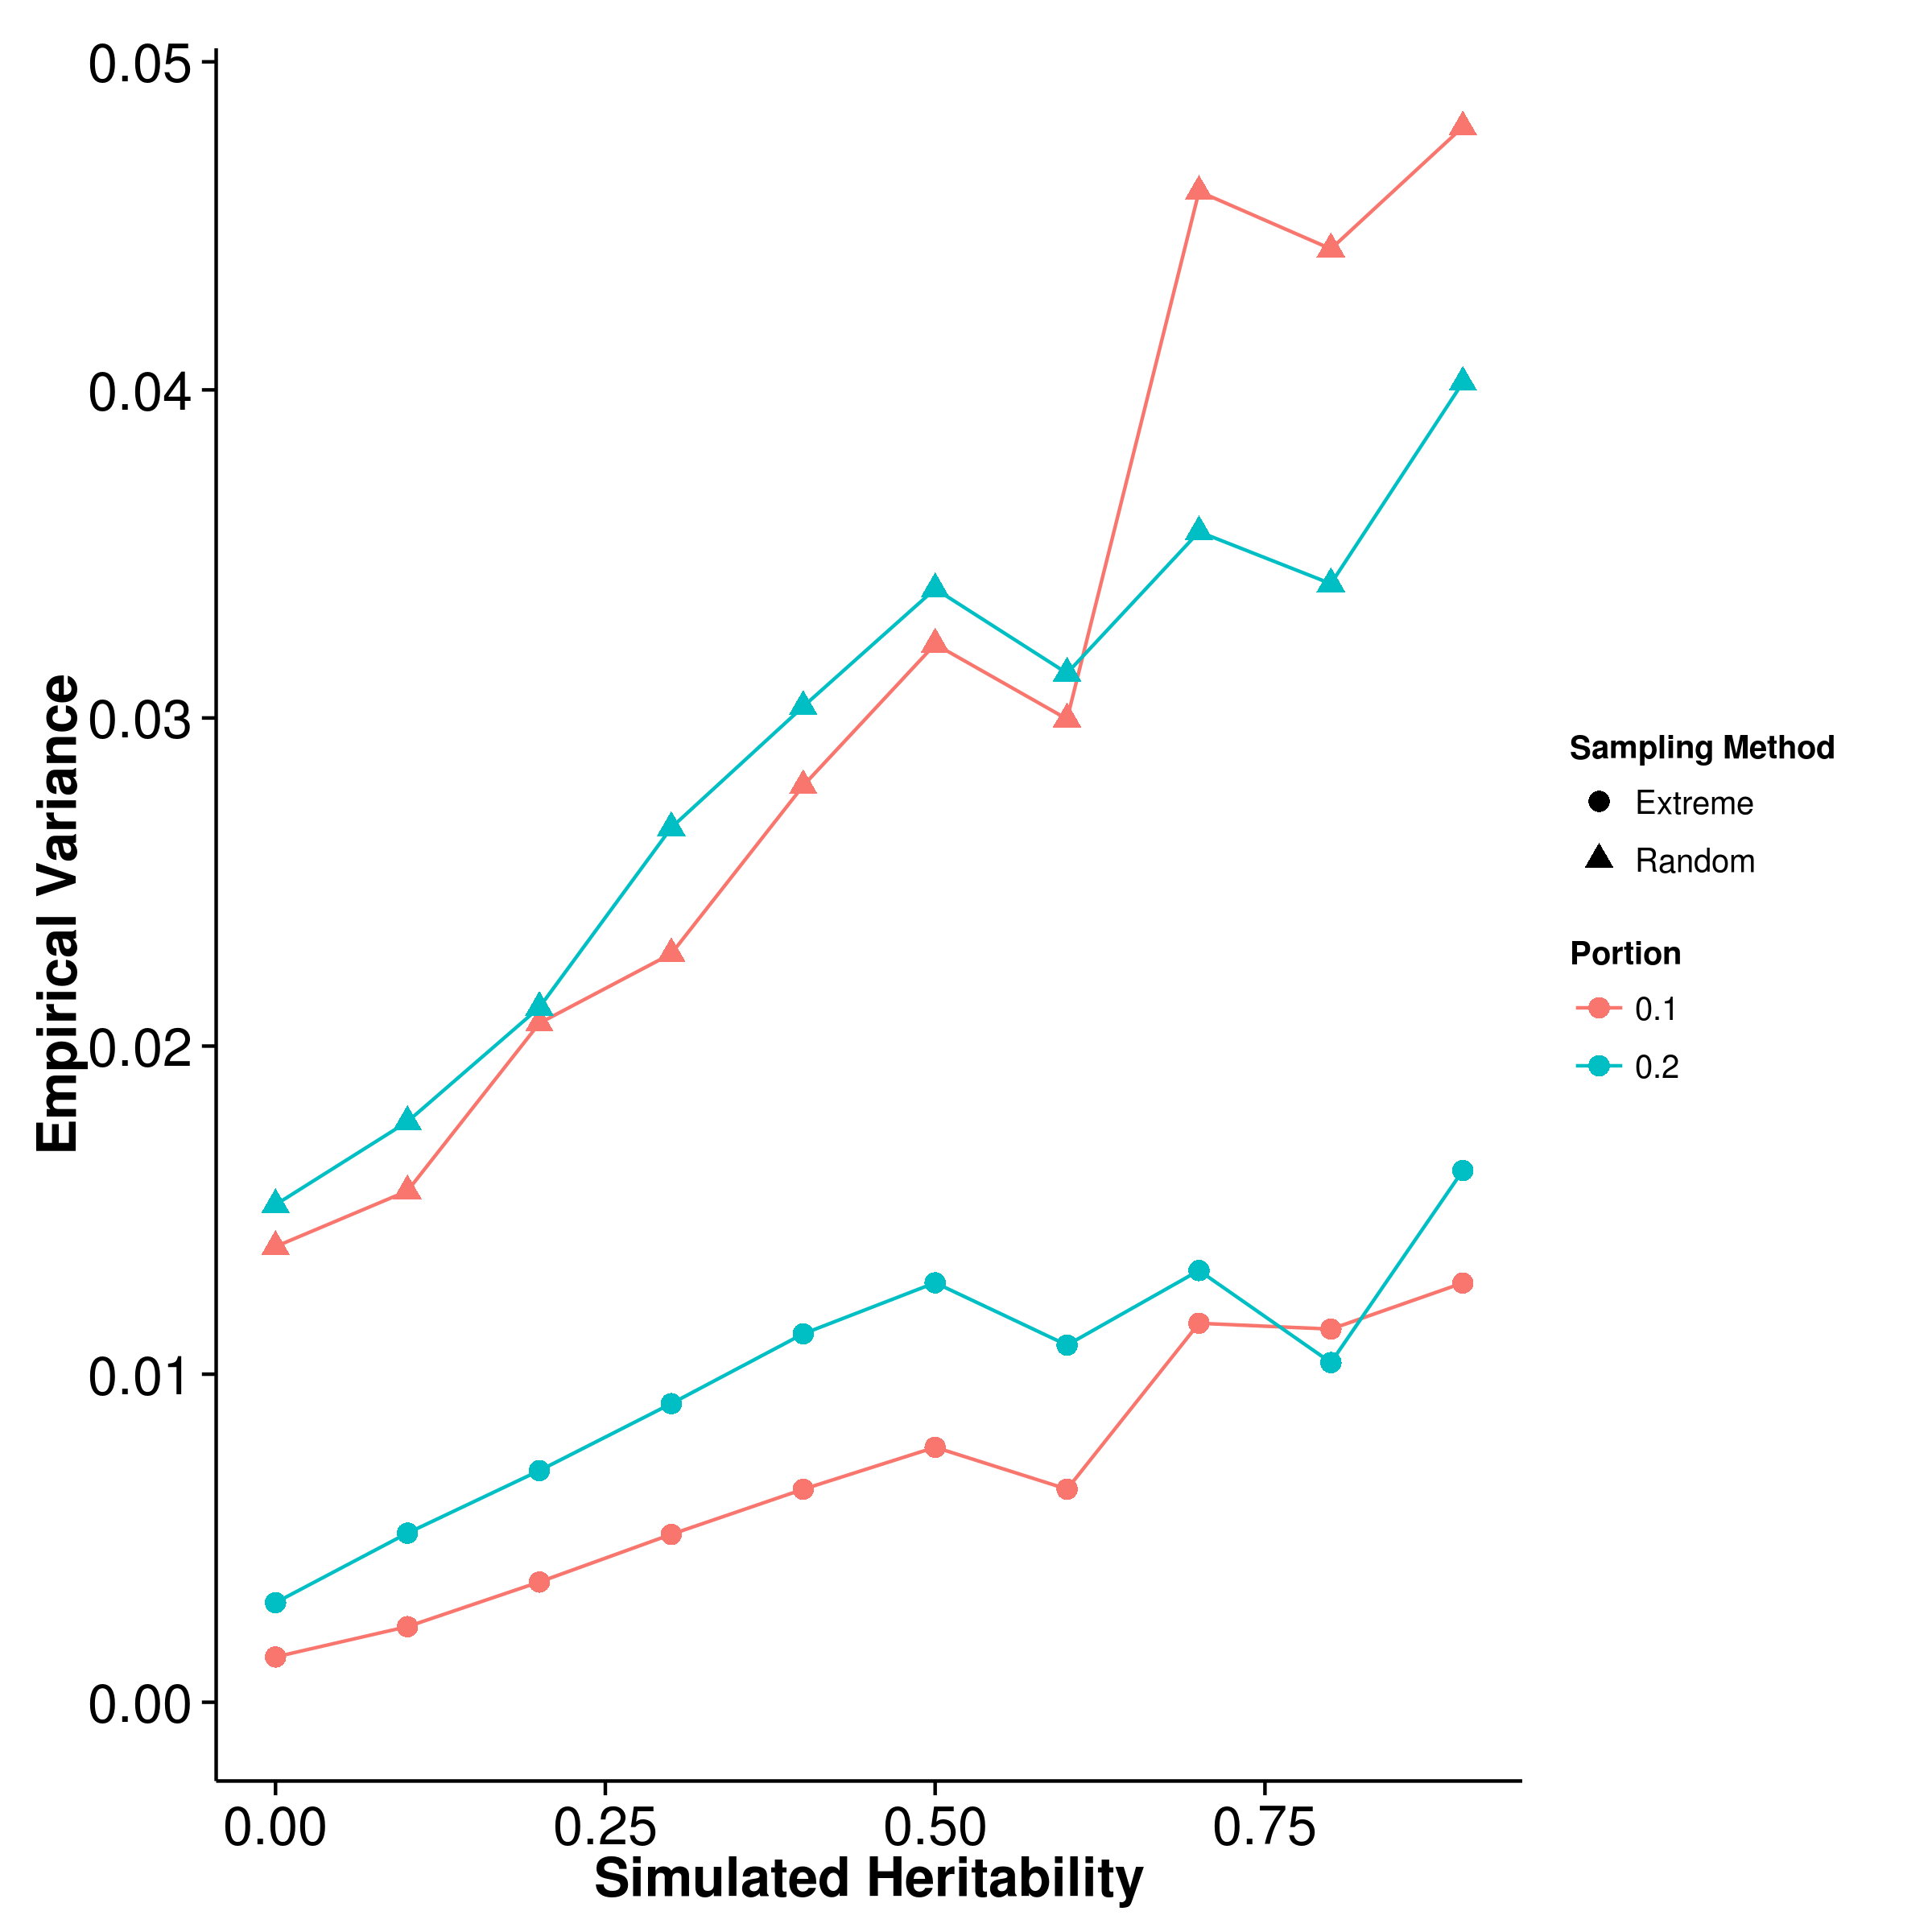
\includegraphics{figure/he_summary/pheno_extreme/ldscIn_extremeSelect_var.png}}
					\label{fig:ldscInExVar}
				}
				\caption[Variance of Extreme Phenotype Selection Simulation Results]
				{Variance of results from extreme phenotype simulation.
					It is obvious that when the extreme phenotype selection was performed, the empirical variance of all the algorithm decreases and is much smaller than the empirical variance of the estimation when random sampling was performed.
					We also compared the empirical variance of random sampling with those from quantitative trait simulation with 100 causal \glspl{SNP} and they are highly similar. 
				} 
				\label{fig:ExVar}
			\end{figure}
			%Variance Estimation
			\begin{figure}
				\centering
				\subfloat[SHREK]{
					\scalebox{.4}{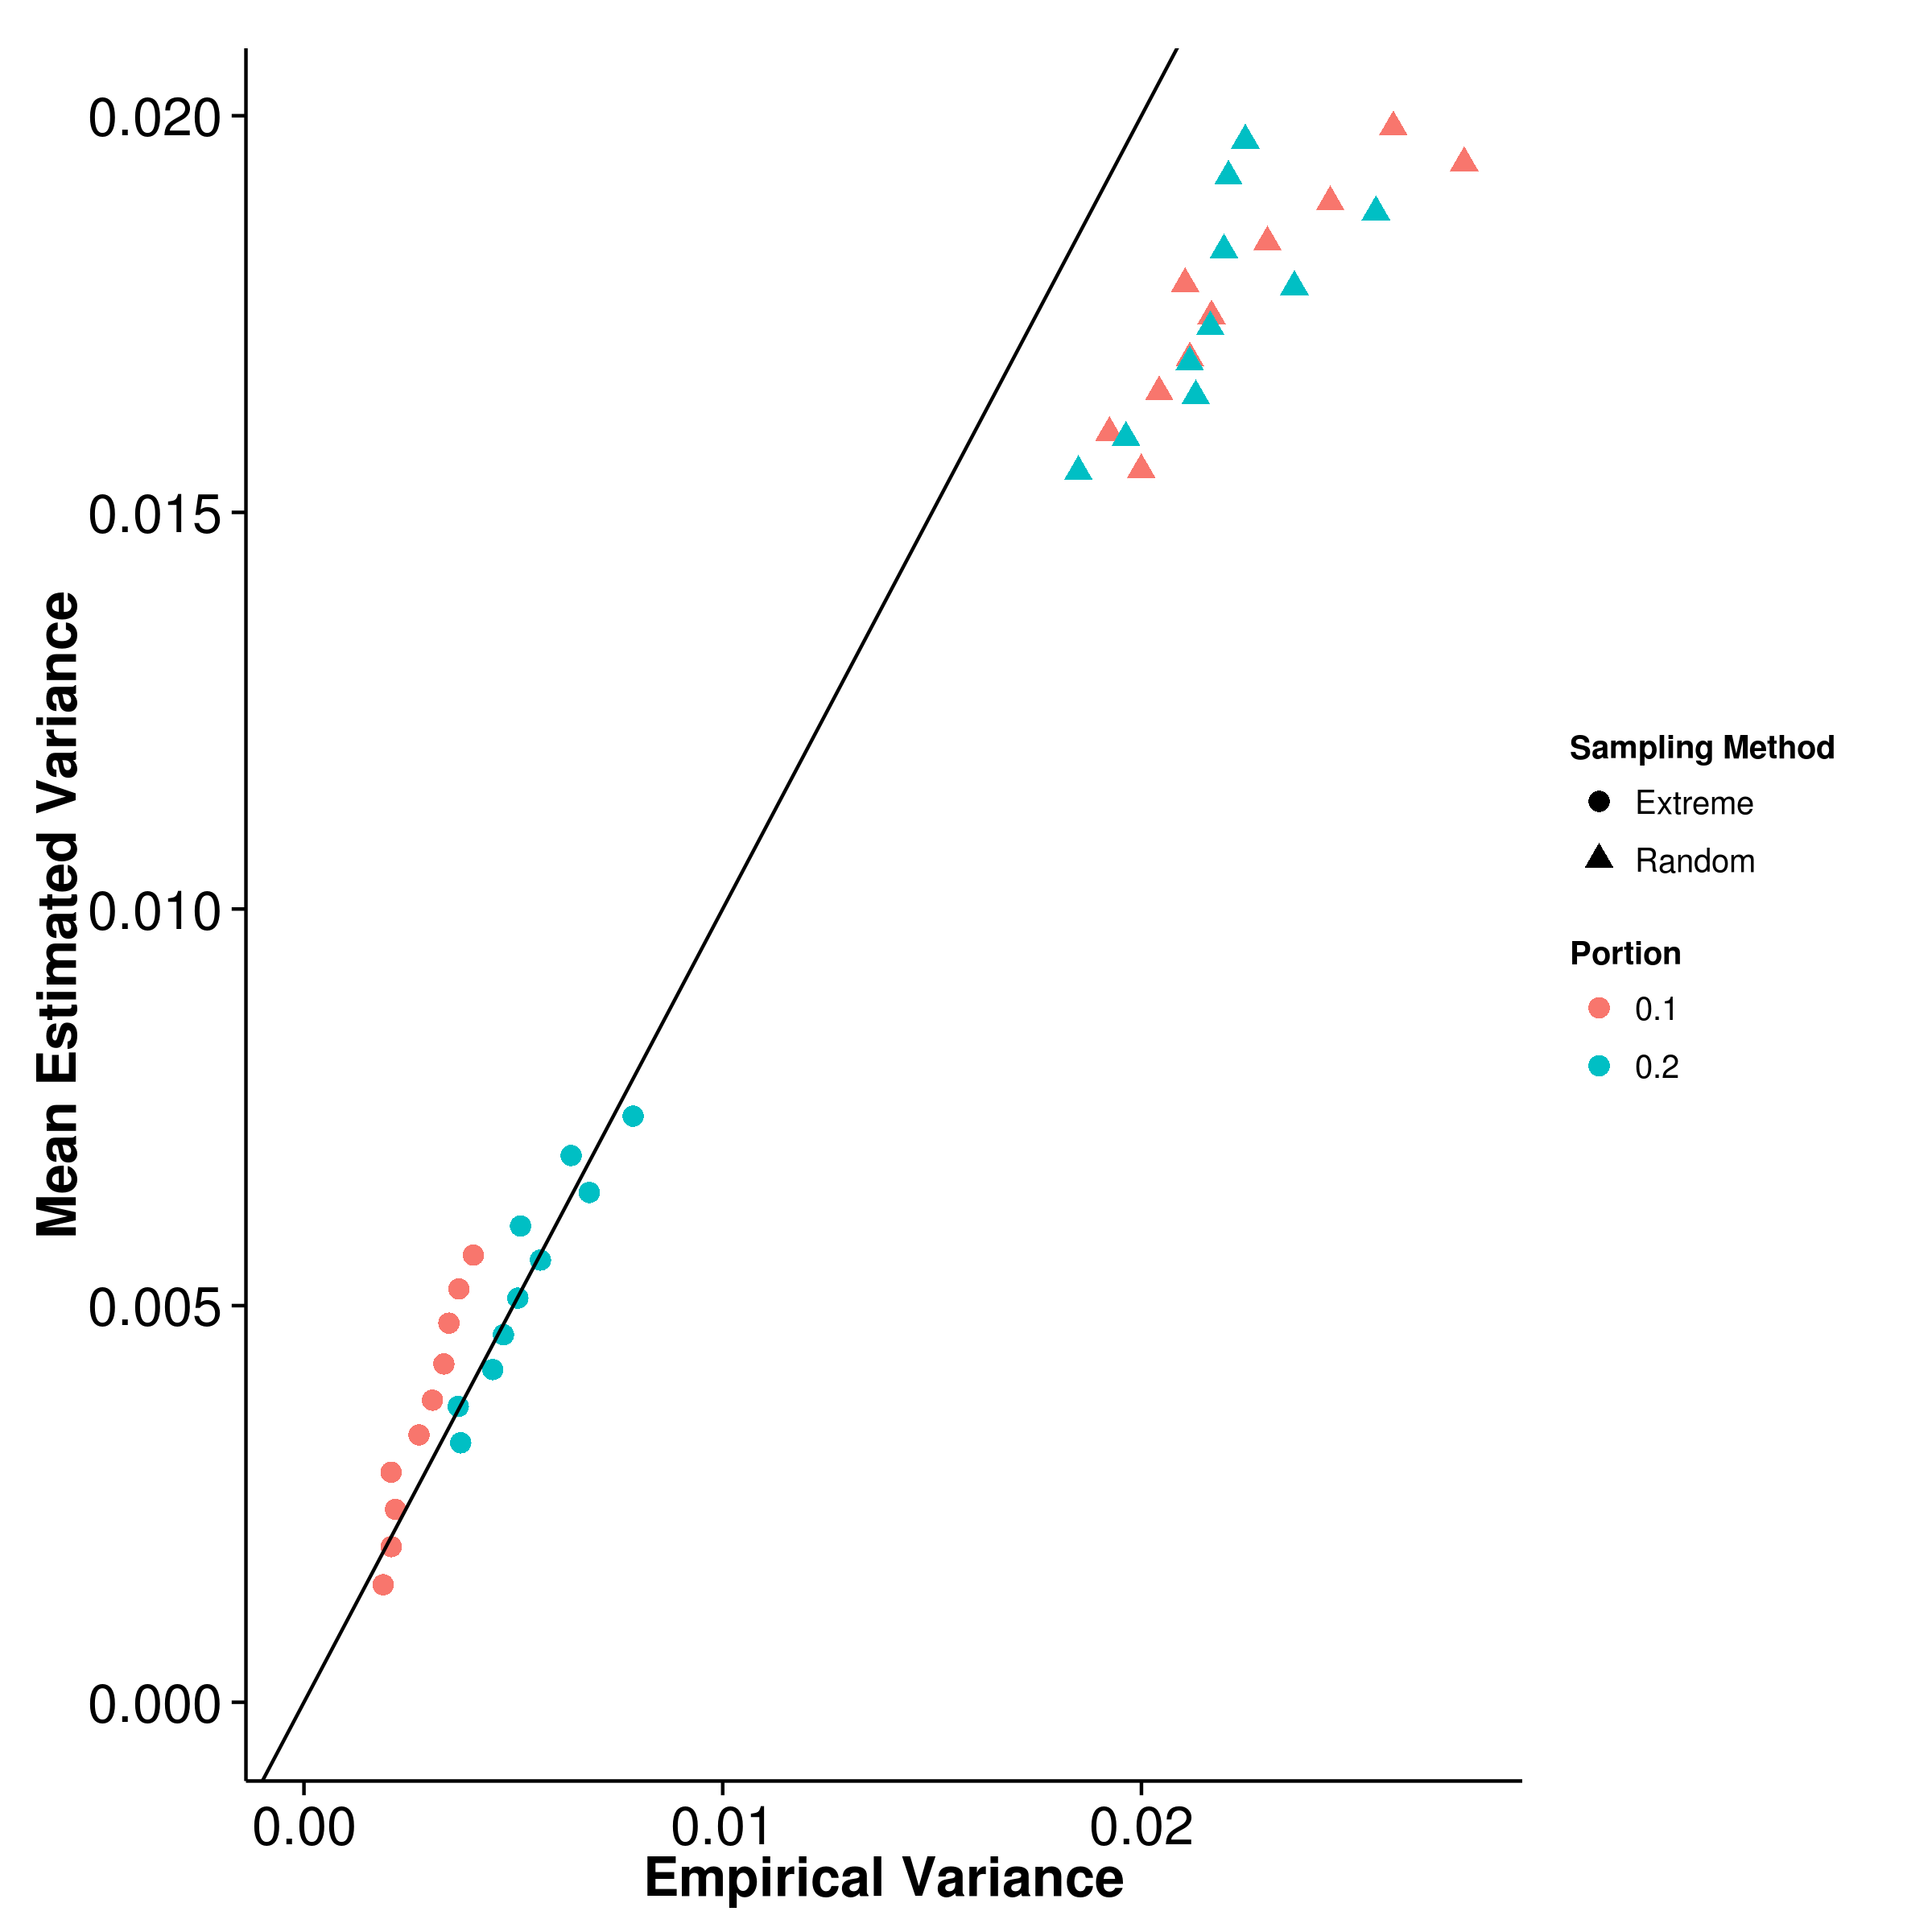
\includegraphics{figure/he_summary/pheno_extreme/shrek_extremeSelect_varCom.png}}
					\label{fig:shrekExVarCom}
				}
				\subfloat[GCTA]{
					\scalebox{.4}{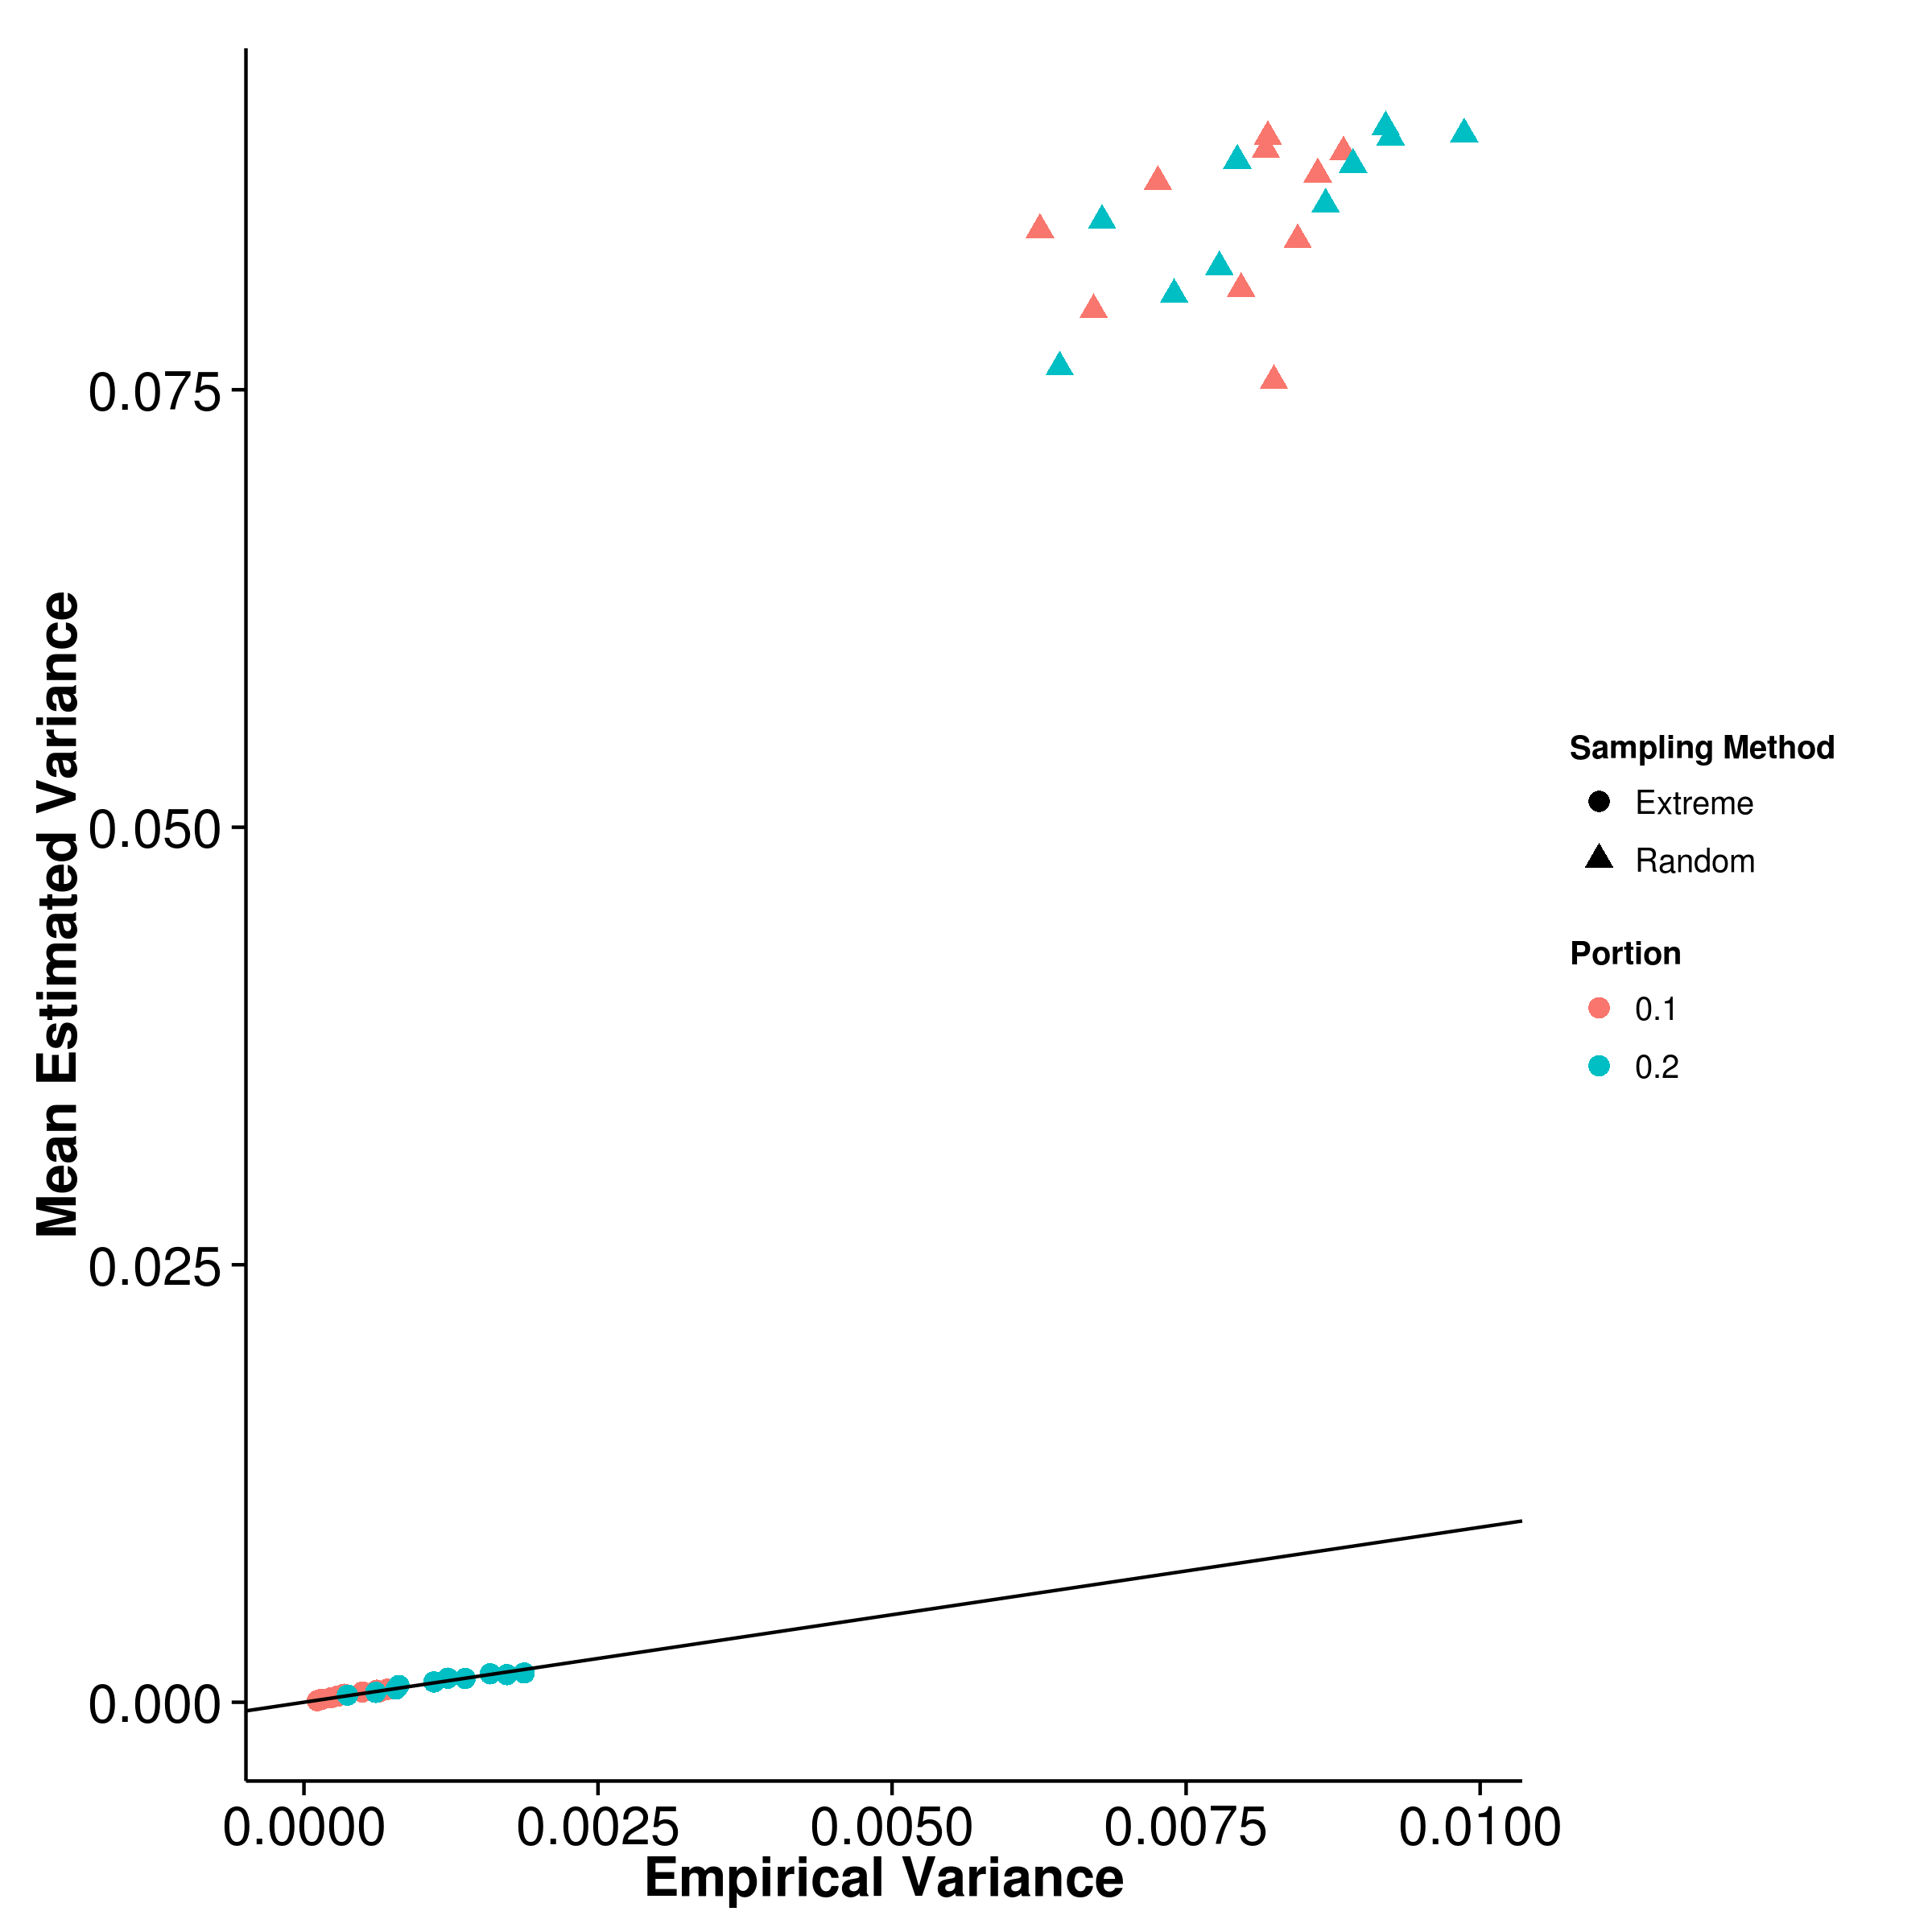
\includegraphics{figure/he_summary/pheno_extreme/gcta_extremeSelect_varCom.png}}
					\label{fig:gctaExVarCom}
				}\\
				\subfloat[LDSC with fix intercept]{
					\scalebox{.4}{\includegraphics{figure/he_summary/pheno_extreme/ldsc_extremeSelect_varCom.png}}
					\label{fig:ldscExVarCom}
				}
				\subfloat[LDSC with intercept estimation]{
					
					\scalebox{.4}{\includegraphics{figure/he_summary/pheno_extreme/ldscIn_extremeSelect_varCom.png}}
					\label{fig:ldscInExVarCom}
				}
				\caption[Estimation of Variance in Extreme Phenotype Selection]
				{Estimated variance of results from extreme phenotype selection when compared to empirical variance.
					Surprisingly, except for \gls{shrek}, the estimated variance from \gls{ldsc} and \gls{gcta} under the random sampling condition was much higher than the empirical variance. 
					It is much different from the estimated variance from the quantitative trait simulation and further investigations are required to understand this discrepancy.
				} 
				\label{fig:ExVarCom}
			\end{figure}
			
		By using appropriate sampling strategy, such as that of extreme phenotype sampling \citep{Peloso2015}, one can increase the power of the association study.
		However, it is unclear how the extreme phenotype sampling will affect the performance of the \gls{SNP} heritability estimation.
		Therefore, simulations were performed to investigate the effect of extreme phenotype sampling on \gls{SNP} heritability estimation compared to random sampling approach. 
		
		It is observed that when the extreme phenotype sampling was performed, the estimates from \gls{gcta} biased downward in pattern similar to what has been observed in the case control simulation (\cref{fig:gctaExMean}).
		On the other hand, estimates from \gls{shrek} and \gls{ldsc} with fixed intercepts are slightly inflated whereas \gls{ldsc} with intercept estimation slightly underestimated the \gls{SNP} heritability (\cref{fig:ExMean}).
		
		When comparing the empirical variance, the random sampling consistently results in a larger empirical variance in the estimates of the algorithms (\cref{tab:ratioEx}).	
		It is observed that when random sampling were performed, the resulting empirical variance from the algorithms are similar to the results in the quantitative trait simulation. 
		However, there is a large discrepancy in the estimated variance of \gls{ldsc} and \gls{gcta}, where there can be as much as a tenfold difference (\cref{fig:ExVarCom}). 
		On the other hand, the estimated variance of \gls{shrek} is unaffected.
		It is unclear what induces the inflation and further investigations are therefore required.
		
		\begin{table}[H]
			\centering
			\begin{tabular}{rrrrrrrrr}
				\toprule
				\multirow{2}[4]{*}{Portion} & \multicolumn{2}{c}{Shrek} & \multicolumn{2}{c}{LDSC} & \multicolumn{2}{c}{LDSC-In} & \multicolumn{2}{c}{GCTA} \\
				& Extreme & Rand & Extreme & Rand & Extreme & Rand & Extreme & Rand\\
				\midrule
				0.1   & 0.0113 & 0.0341 & 0.00537 & 0.0167 & 0.0119 & 0.0329 & 0.0644 & 0.00849 \\
				0.2   & 0.0109 & 0.0290 & 0.00599 & 0.0152 & 0.0126 & 0.0299 & 0.0274 & 0.00852 \\
				\bottomrule
			\end{tabular}
			\caption[Comparing the MSE of Extreme Phenotype Sampling and Random Sampling]{
				Comparing the \gls{mse} of extreme phenotype sampling (Extreme) and random sampling (Rand).
				With the exception of \gls{gcta}, the extreme phenotype sampling will results in a smaller \gls{mse} given the same amount of samples.
			}
			\label{tab:ratioEx}
		\end{table}
		
		%\subsection{Real Data Simulation}
		% Can't explain the results very well
		% Main problem is the reference panel
		
		\subsection{Application to Real Data}
		It is estimated that the heritability for major depression disorder is around 0.252 by \gls{shrek} and 0.154 by \gls{ldsc} with intercept estimation (\gls{ldsc}-In) whereas the heritability of bipolar is estimated to be around 0.308 by \gls{shrek} and 0.181 by \gls{ldsc}-In (\cref{tab:realData}).
		For \glng{scz}, the heritability is estimated to be around 0.185 by \gls{shrek} and 0.135 by \gls{ldsc}-In.
		It is observed that the estimates from \gls{ldsc} with fixed intercept and \gls{shrek} are generally larger than the estimates from \gls{ldsc} with intercept estimation (\gls{ldsc}-In) (\cref{tab:realData}).
		Moreover, the \gls{SNP} heritability estimated for \glng{scz} is much smaller than previously reported by \citet{Bulik-Sullivan2015}.
		Our results indicated that the common \glspl{SNP} have relatively less contribution to the genetic predisposition of individuals to \glng{scz} as measured by the heritability estimated. 
		It is possible for genetic variations such as epigenetics and rare variants to account for the remaining heritability of \glng{scz}.
		\begin{table}[H]
			\centering
			\begin{tabular}{rrrr}
				\toprule
				 \\
				& Major Depression Disorder & Bipolar & \Glng{scz}\\
				\midrule
				%\gls{shrek}   & 0.256 (0.0273)  & 0.312 (0.0168)  & 0.174 (0.00453) \\
				%\gls{ldsc}   & 0.235 (0.0241) & 0.267 (0.0147) & 0.197 (0.0058)\\
				%\gls{ldsc}-In   & 0.161 (0.0317) & 0.185 (0.0211) & 0.133 (0.0071)\\			
				\gls{shrek} & 0.252 (0.0273)& 0.308 (0.0167) & 0.185 (0.00450) \\ 
				\gls{ldsc} & 0.232 (0.0217) & 0.265 (0.0152) & 0.198 (0.0057) \\				\gls{ldsc}-In & 0.154 (0.033) & 0.181 (0.0203) & 0.135 (0.0072) \\
				\bottomrule
			\end{tabular}
			\caption[Heritability Estimated for PGC Data Sets]{
				Heritability estimated for \gls{pgc} data sets.
				The heritability estimated from \gls{ldsc} when intercept estimation was performed (\gls{ldsc}-In) are lower than the estimates from \gls{shrek} and \gls{ldsc} with fixed intercept.
				As the intercept estimation was used for the correction of confounding effects such as population stratifications or cryptic relatedness, the larger estimates from \gls{shrek} and \gls{ldsc} might be a result of the confounding effects.
			}
			\label{tab:realData}
		\end{table}
		
	\section{Discussion}
	The development of \gls{GWAS} allow the systematic association of common genetic variants, such as \glspl{SNP}, to traits on a genome-wide scale.
	In a recent \gls{GWAS} conducted by the \gls{pgc}, 108 genetic loci were found to be associated with \glng{scz} \citep{Ripke2014}.
	Despite the success of the \gls{pgc} \glng{scz} \gls{GWAS}, it is uncertain whether if common genetic variants such as \glspl{SNP} are the main contribution to individual differences in the liability to \glng{scz}.
	Therefore, estimating the contribution of the common \glspl{SNP} included in the \gls{GWAS}, to \glng{scz} has important implications for future research strategy. 
	
	The contribution of common \glspl{SNP} to the heritability of a disease (\gls{SNP} heritability) were usually performed using \gls{gcta}, which relies on the genetic relationship matrix.
	However, the calculation of genetic relationship matrix requires the sample genotypes.
	The sample genotypes are usually unavailable due to privacy concerns.
	Instead, summary statistics from the association analysis are usually available.

	To our knowledge, \gls{ldsc} and \gls{shrek} are the first algorithms that allows the estimation of \gls{SNP} heritability using only the summary statistics from a \gls{GWAS}.
	With \gls{ldsc} and \gls{shrek}, it is now possible to estimates the \gls{SNP} heritability from the \gls{pgc} \glng{scz} \gls{GWAS}, which only the summary statistics of the association is available.
	The \gls{SNP} heritability of \glng{scz} should provide vital information to the future research direction of \glng{scz}.
	
	
	In this chapter, a series of extensive simulation analyses were performed to examine the effect of different sampling strategies and genetic architectures on the performance of \gls{ldsc} and \gls{shrek}.
	The \gls{SNP} heritability of \glng{scz} were also estimated using the \gls{pgc} \glng{scz} \gls{GWAS} summary statistics.
	
	\subsection{LD Correction}
	First, because \gls{shrek} heavily relies on the \gls{LD} information for the estimation of \gls{SNP} heritability, it is important to obtain an accurate estimation of \gls{LD}.
	However, because the reference panels are a subsets of the population, sampling error exists in the estimated \gls{LD}.
	When taking the square of \gls{LD}, a positive bias is observed, which can affect the estimation of \gls{SNP} heritability.
	
	It is observed that of all the bias correction algorithms from \cref{sec:ldSim}, the  equation from \citet{Weir1980} \cref{eq:weir} has the best performance. 
	Therefore, it was selected as the default bias correction algorithm.
	
	By applying the bias correction algorithm, a more accurate estimates were expected to be obtained.
	However, in the quantitative trait simulation, an upward bias is consistently observed in the estimates from \gls{shrek}.
	From the \gls{LD} correction simulation, it is observed that the \gls{LD} correction algorithms may cause an inflation in the estimates.
	As the number of simulated \glspl{SNP} is much smaller in the \gls{LD} correction simulation when compared to the quantitative trait simulation, it is possible for the increased number of \glspl{SNP} to increase the magnitude of bias.
	
	Moreover, although \gls{ldsc} also relies on the \gls{LD} information, the same overestimation is not observed.
	Upon detail inspection of \gls{ldsc}, it is observed that \gls{ldsc} employed a different \gls{LD} correction algorithm:
	\begin{equation}
	\text{LDSC}: \tilde{R^2}= \hat{R^2}-\frac{1-\hat{R^2}}{n-2}\label{eq:ldscR2} 
	\end{equation}
	
	Given these information, it is important to investigate the performance of the \gls{LD} correction algorithms when a larger number of \glspl{SNP} are simulated (e.g. 50,000 \glspl{SNP} on chromosome 1).
	The \gls{LD} correction simulation was therefore repeated.
	Instead of simulating 5,000 \glspl{SNP} from chromosome 22, 50,000 \glspl{SNP} were simulated from chromosome 1. 
	As most \gls{LD} correction from \cref{sec:ldSim} produced similar results in previous simulation, only \cref{eq:ldscR2}, \cref{eq:weir} and \cref{eq:pratt} were included in this scaled up simulation.
	\begin{figure}[t]
		\centering
		\subfloat[Mean Estimation]{
			\scalebox{.4}{\includegraphics{figure/quantitative/ld_correct/ldCom_mean_b.png}}
			\label{fig:bigmeanLDCor}
		}
		\subfloat[Empirical Variance]{
			\scalebox{.4}{\includegraphics{figure/quantitative/ld_correct/ldCom_var_b.png}}
			\label{fig:bigvarLDCor}
		}
		\caption[Effect of LD correction to Heritability Estimation with 50,000 SNPs]
		{Effect of LD correction to Heritability Estimation when 50,000 \glspl{SNP} were simulated.
			It is observed that all \gls{LD} correction algorithms inflate the estimates when large number of \glspl{SNP} were simulated.
			Interestingly, least amount of bias is observed when no \gls{LD} correction was performed.
		} 
		\label{fig:ldCorBigCom}
	\end{figure}
	
	It is clear from \cref{fig:ldCorBigCom} that all \gls{LD} correction algorithms inflate the estimates from \gls{shrek}, whereas a small downward bias is observed in the estimates when no \gls{LD} correction was performed.
	Interestingly, when inspecting the \gls{mse} of the estimates, \gls{shrek} produced the best estimates when no \gls{LD} correction was performed.
	This results suggest that as the number of \glspl{SNP} increases, the \gls{LD} correction algorithms might have a negative impact to the performance of \gls{shrek}.
	One possible explanation is that small imprecisions might be introduced to the \gls{LD} when the sampling error is being adjusted.
	As the number of \glspl{SNP} increases, the imprecisions accumulates, therefore leading to bias in the estimates of \gls{shrek}.
	
	Another interesting observation is that when the \gls{LD} correction algorithm from \gls{ldsc} was applied to \gls{shrek}, the estimates were upwardly biased.
	As the same inflation was not observed in the estimates from \gls{ldsc}, this suggest that \gls{shrek} maybe more sensitive to errors within the \gls{LD} matrix when compared to \gls{ldsc}.
	It is noted that the algorithm of \gls{shrek} requires the inverse of the \gls{LD} matrix. 
	Because the \gls{LD} matrix is ill-conditioned, \gls{shrek} is prone to large numerical errors.
	On the other hand, \gls{ldsc} does not require to invert the \gls{LD} matrix, therefore it is more numerically stable.
	Therefore, because of the fundamental difference in the two numerical methods, \gls{shrek} is more sensitive to errors when compared to \gls{ldsc}.
	

	\subsection{Simulation Results}
	The main goal of the current study is to understand the impact of different sampling strategies and different genetic architectures on the performance of the \gls{SNP} heritability estimation algorithms.
	A series of extensive simulations were therefore performed.
	
	\subsubsection{Quantitative Trait Simulation}
	From the quantitative trait simulation, it is observed that \gls{gcta} has the best overall performance. 
	However, the main problem of \gls{gcta} is that it requires the sample genotypes for the calculation of the genetic relationship matrix.
	When the sample genotypes are unavailable, \gls{gcta} cannot be performed. 
	On the other hand, \gls{ldsc} and \gls{shrek} can still estimate the \gls{SNP} heritability given only the summary statistics from a \gls{GWAS} and a reference panel for the estimation of \gls{LD}.
	
	Similar to the results from \citet{Bulik-Sullivan2015}, we observed that the variance of \gls{ldsc} increases as the number of causal \glspl{SNP} decrease. 
	It is also observed that when the intercept estimation was performed, the variance of \gls{ldsc} increases.
	On the other hand, although the variance of estimates from \gls{shrek} also increases as number of causal \glspl{SNP} decrease, the magnitude of increase is much smaller, suggesting that \gls{shrek} is robust against change in number of causal \glspl{SNP}.
	As a result, when the number of causal \glspl{SNP} are small, \gls{shrek} will provide a more stable result.
	
	Sometimes, it is possible for a small number of causal \gls{SNP}(s) to have a larger effect size when compared to other causal \glspl{SNP}.
	It is observed that only in the extreme scenario where 1 of the causal \gls{SNP} was simulated with a larger effect size will the performance of \gls{ldsc} be affected.
	However, upon re-examination of \cref{eq:extremEffect} which was used for the simulation of \glspl{SNP} with extreme effect size, it is noted that an unnecessary upper bound of ($h^2$) was imposed to the effect sizes.
	A better alternative maybe to first simulate the effect sizes using \cref{eq:randomEffect}.
	Then, for the $m$ ``extreme'' \gls{SNP}(s), their effect sizes should be multiplied with a large constant (e.g 10).
	When compared to \cref{eq:extremEffect}, this should ensure the effect size(s) of the ``extreme'' \gls{SNP}(s) to be larger than other causal \glspl{SNP}.
	As a result, we are currently repeating the simulation from \cref{sec:extremeEffectSim} to investigate the effect of the presence of a small number of causal \glspl{SNP} with large effect size to the performance of the algorithms.
	
	Although the effect of number of causal \glspl{SNP}, trait heritability and the impact of having small number of causal \gls{SNP}(s) with large effect size were considered, the effect of confounding factors on the performance of the algorithms was not examined.
	Therefore, it is uncertain how the performance of \gls{shrek} and \gls{ldsc} will be affected by the presence of confounding factors.
	Specifically, the core concept of the intercept estimation in \gls{ldsc} is to delineate the contribution from confounding factors and common genetic variants.
	It is therefore expected that when confounding factors are presented, \gls{ldsc} with the intercept estimation might outperform \gls{shrek} and \gls{ldsc} with fixed intercept.
	
	However, it is difficult to simulate confounding factors such as population stratification and cryptic relatedness.
	To our knowledge, there are no readily available softwares for the simulation of cryptically related samples.
	On the other hand, although it is possible to simulate stratified samples, a multitude of factors can confound the simulation with population stratification.
	The selection of reference panel is by far the most important factor to consider. 
	For example, if half of the samples were simulated based on European samples and the remaining half of the samples were simulated based on African samples, then it is unclear whether if the European samples or the African samples should be used as the reference panel.
	Moreover, common practice in \gls{GWAS} analysis is to adjust for the population stratification either using \gls{pca} or EIGENSTRAT \citep{Price2006}.
	With the additional adjustment, the properties of the summary statistics will differ, and might therefore affect the \gls{SNP} heritability estimation.
	As a result, to investigate the effect of population stratification, more factors have to be considered, e.g. different reference panel, different proportion of population included, different adjustment methods (e.g. \gls{pca} or EIGENSTRAT) e.t.c.
	Due to the complexity and scope of the problem, it is still a work in progress for us to investigate how the confounding factors affect the performance of \gls{ldsc} and \gls{shrek}.
		
	Overall, our results suggest that \gls{shrek} only outperform \gls{ldsc} in extreme scenarios such as when the trait is oligogenic or when only 1 of the causal \gls{SNP} has large effect size.
	In more general scenarios, the estimates of \gls{ldsc} have a smaller variance and bias when compared to estimates from \gls{shrek}.
	However, it is noted that when no \gls{LD} correction were performed, the bias observed in \gls{shrek} reduced (e.g. from 0.0217 to 0.0166 in the \gls{LD} correction simulation with 50,000 \glspl{SNP} simulated).
	Therefore, when large amount of \glspl{SNP} were simulated, the performance of \gls{shrek} can be improved by not performing the \gls{LD} correction.
	Without the \gls{LD} correction, performance of \gls{shrek} may be comparable to \gls{ldsc} under the polygenic scenario.
	Nonetheless, the sensitive to errors in the \gls{LD} matrix remains to be one of the biggest weakness of \gls{shrek}.
	
	\subsubsection{Case Control Simulation}
	In order to estimate heritability from case control samples, it is important to correct for the ascertainment bias.
	Nevertheless, the correction of ascertainment bias are nontrivial and often introduce bias to the estimates. 
	For example, \citet{Golan2014} observed that \gls{gcta} underestimates the heritability explained by common variants for discontinuous traits.
	The magnitude of this bias is affected by the population prevalence of the trait, the observed prevalence, the true underlying heritability and the number of genotyped \glspl{SNP} \citep{Golan2014}.	
	According to \citet{Golan2014}, there is an oversampling of the cases relative to their prevalence in the population in case control studies.
	The case control sampling induced a positive correlation between the genetic and environmental effects for the samples in the study even when there is no true genetic and environmental interaction in the population \citep{Golan2014}.
	This leads to the estimates from \gls{gcta} to be strongly downward biased where the magnitude of bias increases as the population prevalence decreases, heritability increases and when the proportion of cases is closer to half.

	It is therefore important to investigate whether if \gls{shrek} and \gls{ldsc} are affected in a similar way.
	In our simulation, the same bias is observed for \gls{gcta}, whereas for \gls{shrek} and \gls{ldsc}, an inflation is observed in the estimates when the population prevalence is small.
	As the population prevalence decreases, the magnitude of bias increases, suggesting that the population prevalence has a major influence to the estimates of \gls{ldsc} and \gls{shrek}.
	
	Surprisingly, by applying the intercept estimation, the estimates of \gls{ldsc} becomes more robust to the change in population prevalence (\cref{fig:ldscInCC10RandMean,fig:ldscInCC50RandMean,fig:ldscInCCRandMean,fig:ldscInCC500RandMean}).
	It was expected that as no confounding factors were simulated, the intercept estimation function will be redundant.
	However, results suggest that in the estimation fo \gls{SNP} heritability from case control samples, the intercept estimation might be beneficial even when no confounding factors were presented.
	When population prevalence is small (e.g $<0.05$), the performance of \gls{ldsc} is better when the intercept estimation was performed even without the presence of any confounding factors \cref{tab:mseCC}.
	Further investigation are required to understand how the intercept estimation can improve the performance under the case control scenario.
	This might provide insight for the development of a better algorithm in the estimation of \gls{SNP} heritability from case control samples for \gls{ldsc} and \gls{shrek}.
	
	\subsubsection{Extreme Phenotype Sampling}
	When budgets are limited, extreme phenotype sampling might help to increase the power of the association study given the same amount of samples. 
	Compared with the same number of randomly selected individuals, the extreme selection design can increase the power by a factor of $\frac{V_{P'}}{V_P}$ where $V_{P'}$ is variance of the trait of the selected sample and $V_P$ is the trait variance of the general population.
	So for example, if one only include the samples from the top 5\% and bottom 5\% of the phenotype distribution, one can achieve the same power as a study with random sampling design that has 4 times the sample size \citep{Sham2014}. 
	
	\begin{figure}[t]
		\centering
		\subfloat[No Extreme sampling]{
			\scalebox{.4}{\includegraphics{figure/noSelection.png}}
			\label{fig:noselect}
		}
		\subfloat[Extreme Sampling]{
			\scalebox{.4}{\includegraphics{figure/select.png}}
			\label{fig:selected}
		}
		\caption[Effect of Extreme Sampling Design]
		{Effect of extreme sampling design.
			Although the genetic and environmental effect were simulated independently, an artificial correlation is observed when extreme phenotype sampling was performed. 
			This lead to a downward bias in the estimates from \gls{gcta} \citep{Golan2014}.
		} 
		\label{fig:extremeSampling}
	\end{figure}
	
	Interestingly, it is observed that when extreme phenotype sampling was performed, the estimates from \gls{gcta} are biased downward, similar to the bias observed in the case control simulation.
	The bias observed in \gls{gcta} might be a result of artificial correlation between genetic and environmental effects introduced by extreme phenotype sampling (\cref{fig:extremeSampling}), which is similar to the case control scenario.
	Therefore, as a smaller portion of samples were selected from the extreme ends of a population, the magnitude of bias observed in estimates of \gls{gcta} might increase.
	
	On the other hand, an upward bias is observed in the estimates from \gls{shrek} and \gls{ldsc} when extreme phenotype sampling was performed. 
	The bias is slightly higher when a smaller portion of samples were selected from the extreme end.
	The pattern of the bias observed in the extreme phenotype sampling concurs with the bias observed in the case control scenario.
	This suggests that the ascertainment bias introduced by non-random sampling might affect the performance of the algorithms.
	Further investigation are therefore required to identify a better adjustment for the ascertainment bias in order to improve the performance of \gls{ldsc} and \gls{shrek} when extreme phenotype sampling was performed.
	
	Overall, given the same number of samples, performance of \gls{ldsc} and \gls{shrek} are more than 3 fold better when extreme phenotype sampling was performed, suggesting that extreme phenotype sampling improves not only the power of association studies but also the performance for the estimation of \gls{SNP} heritability.
	
	Peculiarly, in the simulation of random sampling, although the empirical variance is the same as what was observed in the quantitative trait simulation, \gls{gcta} and \gls{ldsc} were unable to estimate their empirical variance. 
	The estimated variance from \gls{gcta} and \gls{ldsc} can be more than 10 fold larger than the empirical variance yet the same bias was not observed in the quantitative trait simulation.
	However, in the simulation of random sampling, all parameters are the same as those in the quantitative trait simulation. 
	It is therefore unclear why a different estimated variance are obtained. 
	Nevertheless, as the sampling were only performed \emph{after} the simulation of phenotypes, any difference in performance should be a result of different sampling strategies. 
	Thus it is safe to conclude that extreme phenotype sampling can provide more power for not only the association studies, but also the for \gls{SNP} heritability estimation given the same amount of samples.
	
	Finally, our simulation only considered limited dimension of parameters. 
	For example, only traits with 100 causal \glspl{SNP} were simulated. 
	More simulations should therefore be performed in order to understand the effect of extreme phenotype sampling on the performance of the algorithms. 
	
	\subsection{Application to Real Data}
	When applying \gls{shrek} and \gls{ldsc} to estimate the \gls{SNP} heritability in real data, it is observed that the estimates from \gls{ldsc} is much smaller than the estimates from the supplementary materials of \citet{Bulik-Sullivan2015} (e.g. for \glng{scz}, 0.555 compared to 0.135).
	After communicated with the corresponding author \citep{Bulik-Sullivan2015c}, it was confirmed that an older implementation of \gls{ldsc} was used to generate the estimates in the supplementary table.
	Specifically, in the formula of \gls{ldsc}:
	\begin{align}
		\mathrm{E}[\chi^2|l_j] &= Nl_j\frac{h^2}{M}+Na+1 \\
		l_j &= \text{LD score of variant}\ j \notag\\
		N &= \text{Sample Size}\notag\\
		a &= \text{Contribution of confounding biases}\notag\\
		h^2 &= \text{heritability}\notag 
	\end{align}
	$M$ was originally defined as the total number of \glspl{SNP} in the reference panel used to estimated \gls{LD} score.	
	However, in the current version of \gls{ldsc}, $M$ was defined as the number of \glspl{SNP} with \gls{maf}$ >5\%$ in the reference panel used to estimate \gls{LD} score which \citet{Bulik-Sullivan2015} deem more appropriate based on new data they observed after their original paper was published.
	From the caption of the supplementary table, it was stated that ``\dots if the average rare \gls{SNP} explains less phenotypic variance than the average common \gls{SNP}, then a smaller value of $M$ would be more appropriate, and the estimates in the supplementary table will be biased upwards.'' \citep{Bulik-Sullivan2015}.
	This explained the discrepancy between our estimates and the estimates observed in the supplementary table from \citet{Bulik-Sullivan2015}.
	
	It is observed that the estimates from \gls{ldsc} with intercept estimation (\gls{ldsc}-In) is smaller than the estimates from \gls{shrek} and \gls{ldsc} with fixed intercept (\cref{tab:realData}).
	From the case control simulation, it is observed that when the population prevalence is less than 0.5, \gls{ldsc}-In underestimates the \gls{SNP} heritability, whereas \gls{shrek} and \gls{ldsc} with fixed intercept overestimates the \gls{SNP} heritability.
	Therefore it is likely for the estimates from \gls{ldsc}-In and \gls{shrek} to be the lower and upper bound of the true \gls{SNP} heritability respectively. 

	However, in our simulation, confounding effects were not simulated, therefore it is unclear how the algorithms will perform in the presence of confounding effects.
	In the presence of population stratification or cryptic relatedness, spurious associations might be observed, leading to an inflated summary statistics \citep{Zheng2006}.
	It is therefore likely for \gls{shrek} and \gls{ldsc} with fixed intercept to overestimate the true \gls{SNP} heritability in the presence of population stratification or cryptic relatedness.
	
	Moreover, from the \gls{LD} correction simulations, it is noted that estimated from \gls{shrek} biased upward when \gls{LD} correction was performed, especially when large number of \glspl{SNP} were included in the study.
	As \gls{LD} correction was performed when we apply \gls{shrek} to real data, it is likely for \gls{shrek} to provide an upward biased estimate.
	Together, it is very likely for \gls{shrek} to overestimate the true \gls{SNP} heritability, therefore, its estimates should be treated as the upper bound of the true \gls{SNP} heritability. 
	Further development of \gls{shrek} are required to reduce the bias and improve its performance. 
	
	Based on our estimation, the \gls{pgc} \glng{scz} \gls{GWAS} can at most account for $\sim20\%$ of the heritability of \gls{scz}.
	When compared to the heritability estimated from twin studies, there are around $40\%\sim60\%$ of missing heritability unaccounted for. 
	As the \gls{SNP} heritability were only estimated based on the autosomal \glspl{SNP}, it is possible for the sex chromosome to account for some of the ``missing heritability''.
	Different methods exists for the association analysis on the X chromosome where a different summary statistics can be obtained \citep{Wong2014} (Supplementary materials).
	It is therefore difficult to perform the estimation of \gls{SNP} heritability on the X chromosome with only the summary statistics. 
	Further investigation are required before \gls{ldsc} and \gls{shrek} can be applied to estimation the contribution of \glspl{SNP} resides on the sex chromosomes.
	
	On the other hand, as the common \glspl{SNP} do not account for all the heritability of \glng{scz}, other genetic variants such as the rare variants and epigenetic changes might be another possible source of heritability of \glng{scz}.
	
	As \gls{LD} calculated from rare variants usually have a large \gls{se}, \gls{shrek} and \gls{ldsc} cannot accurately estimate the contribution of rare variants to the heritability of a disease. 
	\citet{Bulik-Sullivan2015} reported that when all causal variants of a trait are rare (\gls{maf} $<1\%$), \gls{ldsc} will often generate a negative slope, with the intercept exceeding the mean $\chi^2$ statistic.
	Therefore, further developments are required in order to be able to estimate the true contribution of rare variants to the heritability of \glng{scz}.
	
	On the other hand, it was observed that individuals born to schizophrenic mother has a higher risk of \glng{scz} when compared to individuals born to a schizophrenic father \citep{Riley2006}. 
	It is therefore possible for variations in methylation pattern or genetic mutation in the mitochondria, which are mainly transmitted from the mother \citep{Sutovsky1999}, to contribute to the heritability of \glng{scz}.
	Therefore epigenetic might also have an important role in the etiology of \glng{scz}.

	To conclude, the main advantage of \gls{shrek} is its robustness against different genetic architectures, however, further optimizations are required and will be done soon. 
	Nonetheless, the development of \gls{ldsc} and \gls{shrek} allows the estimation of \gls{SNP} heritability using only summary statistics from \gls{GWAS}.
	By understanding the relative contribution of common variants such as \gls{SNP} to the heritability of a disease, a better research strategy can be developed, thus allow for a better use of research resources.
	
	\subsection{Limitations and Improvements}
	When compared to \gls{ldsc}, \gls{shrek} is significantly slower because the inverse of the \gls{LD} matrix are required.
	When the \gls{SNP} density is high (e.g $>2,000$ \glspl{SNP} in a 1 \gls{mb} region), \gls{shrek} requires a significant amount of time to estimate the \gls{SNP} heritability and in the case of \gls{pgc} \glng{scz} \gls{GWAS} dataset, the \gls{SNP} density was too high, forcing us to use a smaller window size for the estimation.
	A possible improvement to \gls{shrek} will be to use a faster library such as the Armadillo library \citep{Sanderson2010}.
	Armadillo library can be 3 times faster than EIGEN C++ library, which is currently used for the implementation of \gls{shrek}, by utilizing the multi-threading high performance OpenBLAS library for the computation of \gls{SVD}.
	Therefore, by using Armadillo and OpenBLAS in the implementation of \gls{shrek}, the speed of the analysis can be increased.
	However, because of the fundamental nature of the algorithm (requiring the inverse of \gls{LD}), it is expected that \gls{shrek} will be slower in comparison to \gls{ldsc}.
	
	Finally, we acknowledge that more simulations can be performed. 
	For example, the effect of the observed prevalence in case control simulations were not investigated. 
	Also, in the extreme phenotype sampling simulation, traits with different number of causal \glspl{SNP} can also be simulated.
	However, the current simulations have provided a general concept to the effect of different sampling strategies and genetic architecture on the performance of \gls{ldsc} and \gls{shrek}.
%	\newpage
	
\begin{singlespace}
\section{Supplementary}


	\begin{figure}[H]
			\centering
			\subfloat[SHREK]{
				\scalebox{.4}{\includegraphics{figure/he_summary/cc_50c/shrek_CC_Rand_mean.png}}
				\label{fig:shrekCC50RandMean}
			}
			\subfloat[GCTA]{
				\scalebox{.4}{\includegraphics{figure/he_summary/cc_50c/gcta_CC_Rand_mean.png}}
				\label{fig:gctaCC50RandMean}
			}\\
			\subfloat[LDSC with fix intercept]{
				\scalebox{.4}{\includegraphics{figure/he_summary/cc_50c/ldsc_CC_Rand_mean.png}}
				\label{fig:ldscCC50RandMean}
			}
			\subfloat[LDSC with intercept estimation]{
				
				\scalebox{.4}{\includegraphics{figure/he_summary/cc_50c/ldscIn_CC_Rand_mean.png}}
				\label{fig:ldscInCC50RandMean}
			}
			\caption[Mean of Case Control Simulation Results (50 Causal)]
			{Mean of results from case control simulation with random effect size simulation with 50 causal \glspl{SNP}.
				In general, the results were similar to the scenario with 10 causal \glspl{SNP} with the only exception that the estimates from \gls{ldsc} with intercept estimates seems to be less affected by the change in prevalence of the trait.
				} 
			\label{fig:CC50RandMean}
		\end{figure}
		
		\begin{figure}
			\centering
			\subfloat[SHREK]{
				\scalebox{.4}{\includegraphics{figure/he_summary/cc_50c/shrek_CC_Rand_sd.png}}
				\label{fig:shrekCC50RandVar}
			}
			\subfloat[GCTA]{
				\scalebox{.4}{\includegraphics{figure/he_summary/cc_50c/gcta_CC_Rand_sd.png}}
				\label{fig:gctaCC50RandVar}
			}\\
			\subfloat[LDSC with fix intercept]{
				\scalebox{.4}{\includegraphics{figure/he_summary/cc_50c/ldsc_CC_Rand_sd.png}}
				\label{fig:ldscCC50RandVar}
			}
			\subfloat[LDSC with intercept estimation]{
				
				\scalebox{.4}{\includegraphics{figure/he_summary/cc_50c/ldscIn_CC_Rand_sd.png}}
				\label{fig:ldscInCC50RandVar}
			}
			\caption[Variance of Case Control Simulation Results (50 Causal)]
			{Variance of results from case control simulation with random effect size simulation with 50 causal \glspl{SNP}.
				For most algorithm except that of \gls{ldsc} with fixed intercept, the empirical variance of the estimates increases as the population prevalence of the trait increases, with the estimations from \gls{ldsc} with intercept estimation display the largest variance.
			} 
			\label{fig:CC50RandVar}
		\end{figure}
		
		
		\begin{figure}
			\centering
			\subfloat[SHREK]{
				\scalebox{.4}{\includegraphics{figure/he_summary/cc_50c/shrek_CC_Rand_sdCom.png}}
				\label{fig:shrekCC50RandVarCom}
			}
			\subfloat[GCTA]{
				\scalebox{.4}{\includegraphics{figure/he_summary/cc_50c/gcta_CC_Rand_sdCom.png}}
				\label{fig:gctaCC50RandVarCom}
			}\\
			\subfloat[LDSC with fix intercept]{
				\scalebox{.4}{\includegraphics{figure/he_summary/cc_50c/ldsc_CC_Rand_sdCom.png}}
				\label{fig:ldscCC50RandVarCom}
			}
			\subfloat[LDSC with intercept estimation]{
				
				\scalebox{.4}{\includegraphics{figure/he_summary/cc_50c/ldscIn_CC_Rand_sdCom.png}}
				\label{fig:ldscInCC50RandVarCom}
			}
			\caption[Estimation of Variance in Case Control Simulation (50 Causal)]
			{Estimated variance of results from case control simulation with random effect size simulation when compared to empirical variance when 50 causal \glspl{SNP} was simulated.
				Again, the estimation of variance from \gls{shrek} tends to be downwardly biased and \gls{ldsc} with fixed intercept tends to be upwardly biased. 
				However, when intercept estimation was performed, the estimation of variance of \gls{ldsc} improved.
			} 
			\label{fig:CC50RandVarCom}
		\end{figure}
\begin{figure}
			\centering
			\subfloat[SHREK]{
				\scalebox{.4}{\includegraphics{figure/he_summary/cc_100c/shrek_CC_Random_mean.png}}
				\label{fig:shrekCCRandMean}
			}
			\subfloat[GCTA]{
				\scalebox{.4}{\includegraphics{figure/he_summary/cc_100c/gcta_CC_Random_mean.png}}
				\label{fig:gctaCCRandMean}
			}\\
			\subfloat[LDSC with fix intercept]{
				\scalebox{.4}{\includegraphics{figure/he_summary/cc_100c/ldsc_CC_Random_mean.png}}
				\label{fig:ldscCCRandMean}
			}
			\subfloat[LDSC with intercept estimation]{
				
				\scalebox{.4}{\includegraphics{figure/he_summary/cc_100c/ldscIn_CC_Random_mean.png}}
				\label{fig:ldscInCCRandMean}
			}
			\caption[Case Control with Random Effect Size Simulation Result(Mean)]
			{Mean of results from case control simulation with random effect size simulation.
				The performance of \gls{gcta} was as suggested by \citet{Golan2014} where there was an underestimation as prevalence decreases.
				On the other hand, \gls{ldsc} were upwardly biased when a fixed intercept was used and this bias was corrected when an estimation of intercept was allowed.
				\gls{shrek} does not seems to as sensitive to change in prevalence and the estimation were relatively robust.
				} 
			\label{fig:CCRandMean}
		\end{figure}
		
		\begin{figure}
			\centering
			\subfloat[SHREK]{
				\scalebox{.4}{\includegraphics{figure/he_summary/cc_100c/shrek_CC_Random_sd.png}}
				\label{fig:shrekCCRandVar}
			}
			\subfloat[GCTA]{
				\scalebox{.4}{\includegraphics{figure/he_summary/cc_100c/gcta_CC_Random_sd.png}}
				\label{fig:gctaCCRandVar}
			}\\
			\subfloat[LDSC with fix intercept]{
				\scalebox{.4}{\includegraphics{figure/he_summary/cc_100c/ldsc_CC_Random_sd.png}}
				\label{fig:ldscCCRandVar}
			}
			\subfloat[LDSC with intercept estimation]{
				
				\scalebox{.4}{\includegraphics{figure/he_summary/cc_100c/ldscIn_CC_Random_sd.png}}
				\label{fig:ldscInCCRandVar}
			}
			\caption[Case Control with Random Effect Size Simulation Result(Variance)]
			{Variance of results from case control simulation with random effect size simulation.
				It was clear that the prevalence affects the variance of estimation where a larger variance tends to increase the variance of estimation.
				Again, \gls{gcta} has the lowest variance, however, unlike in the quantitative trait simulation, \gls{shrek} has a lower average variance when compared to \gls{ldsc} with fixed intercept.
				Nonetheless, it was important to remember that in case control simulation, a much smaller amount of \glspl{SNP} was used, thus the results was not directly comparable to results from the quantitative simulation.
			} 
			\label{fig:CCRandVar}
		\end{figure}
		
		
		\begin{figure}
			\centering
			\subfloat[SHREK]{
				\scalebox{.4}{\includegraphics{figure/he_summary/cc_100c/shrek_CC_Random_sdCom.png}}
				\label{fig:shrekCCRandVarCom}
			}
			\subfloat[GCTA]{
				\scalebox{.4}{\includegraphics{figure/he_summary/cc_100c/gcta_CC_Random_sdCom.png}}
				\label{fig:gctaCCRandVarCom}
			}\\
			\subfloat[LDSC with fix intercept]{
				\scalebox{.4}{\includegraphics{figure/he_summary/cc_100c/ldsc_CC_Random_sdCom.png}}
				\label{fig:ldscCCRandVarCom}
			}
			\subfloat[LDSC with intercept estimation]{
				
				\scalebox{.4}{\includegraphics{figure/he_summary/cc_100c/ldscIn_CC_Random_sdCom.png}}
				\label{fig:ldscInCCRandVarCom}
			}
			\caption[Case Control with Random Effect Size Simulation Result(Estimated Variance)]
			{Estimated variance of results from case control simulation with random effect size simulation when compared to empirical variance.
				From the quantitative trait simulation with random effect size(\cref{fig:QtRandVarCom}), it was observed that the variance estimation of \gls{shrek} and \gls{gcta} were rater accurate.
				Similarly, in the case control simulation with 100 causal \glspl{SNP}, it was observed that the variance estimation of \gls{shrek} and \gls{gcta} were close to the empirical variance with slight bias.
				A large up-ward bias was observed for \gls{ldsc} with fixed intercept estimation but the bias was less when \gls{ldsc} was allowed to estimate the intercept.s
			} 
			\label{fig:CCRandVarCom}
		\end{figure}
	\begin{figure}
			\centering
			\subfloat[SHREK]{
				\scalebox{.4}{\includegraphics{figure/he_summary/cc_500c/shrek_CC_Rand_mean.png}}
				\label{fig:shrekCC500RandMean}
			}
			\subfloat[GCTA]{
				\scalebox{.4}{\includegraphics{figure/he_summary/cc_500c/gcta_CC_Rand_mean.png}}
				\label{fig:gctaCC500RandMean}
			}\\
			\subfloat[LDSC with fix intercept]{
				\scalebox{.4}{\includegraphics{figure/he_summary/cc_500c/ldsc_CC_Rand_mean.png}}
				\label{fig:ldscCC500RandMean}
			}
			\subfloat[LDSC with intercept estimation]{
				
				\scalebox{.4}{\includegraphics{figure/he_summary/cc_500c/ldscIn_CC_Rand_mean.png}}
				\label{fig:ldscInCC500RandMean}
			}
			\caption[Mean of Case Control Simulation Results (500 Causal)]
			{Mean of results from case control simulation with random effect size simulation with 500 causal \glspl{SNP}.
				Again, a clear pattern of underestimation was observed for \gls{gcta} and \gls{ldsc} with intercept estimation whereas estimations from \gls{shrek} and \gls{ldsc} with fixed intercepts tends to be upwardly biased, with the magnitude of bias increases as the population prevalence decreases.
				} 
			\label{fig:CC500RandMean}
		\end{figure}
		
		\begin{figure}
			\centering
			\subfloat[SHREK]{
				\scalebox{.4}{\includegraphics{figure/he_summary/cc_500c/shrek_CC_Rand_sd.png}}
				\label{fig:shrekCC500RandVar}
			}
			\subfloat[GCTA]{
				\scalebox{.4}{\includegraphics{figure/he_summary/cc_500c/gcta_CC_Rand_sd.png}}
				\label{fig:gctaCC500RandVar}
			}\\
			\subfloat[LDSC with fix intercept]{
				\scalebox{.4}{\includegraphics{figure/he_summary/cc_500c/ldsc_CC_Rand_sd.png}}
				\label{fig:ldscCC500RandVar}
			}
			\subfloat[LDSC with intercept estimation]{
				
				\scalebox{.4}{\includegraphics{figure/he_summary/cc_500c/ldscIn_CC_Rand_sd.png}}
				\label{fig:ldscInCC500RandVar}
			}
			\caption[Variance of Case Control Simulation Results (500 Causal)]
			{Variance of results from case control simulation with random effect size simulation with 500 causal \glspl{SNP}.
				As the number of causal \glspl{SNP} increased to 500, the empirical variance of \gls{shrek} and \gls{ldsc} with fixed intercept converges. 
				However, the empirical variance of \gls{ldsc} with intercept estimations remains high. 
			} 
			\label{fig:CC500RandVar}
		\end{figure}
		
		
		\begin{figure}
			\centering
			\subfloat[SHREK]{
				\scalebox{.4}{\includegraphics{figure/he_summary/cc_500c/shrek_CC_Rand_sdCom.png}}
				\label{fig:shrekCC500RandVarCom}
			}
			\subfloat[GCTA]{
				\scalebox{.4}{\includegraphics{figure/he_summary/cc_500c/gcta_CC_Rand_sdCom.png}}
				\label{fig:gctaCC500RandVarCom}
			}\\
			\subfloat[LDSC with fix intercept]{
				\scalebox{.4}{\includegraphics{figure/he_summary/cc_500c/ldsc_CC_Rand_sdCom.png}}
				\label{fig:ldscCC500RandVarCom}
			}
			\subfloat[LDSC with intercept estimation]{
				
				\scalebox{.4}{\includegraphics{figure/he_summary/cc_500c/ldscIn_CC_Rand_sdCom.png}}
				\label{fig:ldscInCC500RandVarCom}
			}
			\caption[Estimation of Variance in Case Control Simulation (500 Causal)]
			{Estimated variance of results from case control simulation with random effect size simulation when compared to empirical variance when 500 causal \glspl{SNP} was simulated.
				When the trait contains 500 causal \glspl{SNP}, \gls{ldsc} begins to provide a good estimation of its own empirical variance both with and without intercept estimation. 
				On the other hand, \gls{shrek}'s estimation of its own empirical variance remains consistently lower than the true empirical variance.
			} 
			\label{fig:CC500RandVarCom}
		\end{figure}
\end{singlespace}
	